\documentclass[12pt,PhD,a4paper,pdftex,singlespace]{muthesis}
% \documentclass[11pt,a4paper,pdftex]{book}

% Define a boolean which says we are compiling my thesis
\newif\ifthesis
\thesistrue


%% General packages
%% ============================================================

% Add maths commands, symbols and fonts
\usepackage{amsmath}
\usepackage{amssymb}
\usepackage{amsfonts}
\usepackage{amsthm}
\usepackage{mathtools}

% Greek letters in text
\usepackage[euler]{textgreek}


\usepackage{url}                %Support for urls

\usepackage[colorlinks=true, % colour all links black (just using
            linkcolor=black, % colorlinks=false results in boxes around
            citecolor=black, % links)
            filecolor=black,
            urlcolor=black]{hyperref}

\usepackage{xspace} % command for fixing spaces after macros


% Language
% ============================================================
% Support for UTF8 input
\usepackage[utf8]{inputenc}

%% % Handle non-ascii fonts properly, see
%% % http://tex.stackexchange.com/questions/664/why-should-i-use-usepackaget1fontenc
%% \usepackage[T1]{fontenc}
%% % Seems to break searching so I'm not using it...

% Commonly recommend, not sure what it does...
\usepackage[UKenglish]{babel}



%% Page Layout
%% ============================================================
% Paragraphs use a vertical space rather than tabbing
\setlength{\parskip}{\medskipamount}
\setlength{\parindent}{0pt}
\usepackage[hang,flushmargin]{footmisc} % same for footnotes

% Adds a landscape enviroment
\usepackage{lscape}


%% Figure Tweaks
%% ============================================================
\usepackage[pdftex]{graphicx}   %Needed to include pictures

% positioning tweaks
\renewcommand{\topfraction}{0.85}
\renewcommand{\textfraction}{0.1}
\renewcommand{\floatpagefraction}{0.75}

% Italic captions
\usepackage[labelfont=it,textfont=it]{caption}


%% Equations/maths
%% ============================================================
\numberwithin{equation}{chapter} % Number equations by "<chapter>.<number>".

%\usepackage{nath}
% % Prevent line break in the middle of maths except in extreme cases (increse numbers to make line breaking even more unlikely)
% \relpenalty=3000
% \binoppenalty=5000



%% Bibliograpy Tweaks
%% ============================================================

% biblatex setup
\usepackage[backend=biber,
  citestyle=numeric,
  firstinits=true, % Only print initials of first names
  isbn=false,
  doi=false,
  url=true, % for websites, see below for removing it from papers etc.
]{biblatex}

% clear urls for papers, proceedings, books
\AtEveryBibitem{%
  \ifentrytype{article}{%
    \clearfield{url}%
    \clearfield{urldate}%
  }
  {}% no "else" operation
  %
  \ifentrytype{inproceedings}{%
    \clearfield{url}%
    \clearfield{urldate}%
  }
  {}% no "else" operation
  % 
  \ifentrytype{book}{%
    \clearfield{url}%
    \clearfield{urldate}%
  }
  {}% no "else" operation
}


% Add bibtex files
\addbibresource{mendeley_library.bib}

%% % A superscript ciation command
%% \DeclareCiteCommand{\supercite}[\mkbibsuperscript]
%%   {\iffieldundef{prenote}
%%      {}
%%      {\BibliographyWarning{Ignoring prenote argument}}%
%%    \iffieldundef{postnote}
%%      {}
%%      {\BibliographyWarning{Ignoring postnote argument}}}
%%   {\usebibmacro{citeindex}%
%%    \bibopenbracket\usebibmacro{cite}\bibclosebracket}
%%   {\supercitedelim}
%%   {}

%% % Use superscript cite instead of normal ones
%% \let\cite=\supercite



% Section etc. labelling 
% ============================================================

% This goes last because apparently other packages can break cleveref 

% \def\chapterautorefname{Chapter} % capitalise
% \def\sectionautorefname{Section} % capitalise
% \def\subsectionautorefname{Section} % capitalise, say section not subsection

\usepackage[sort&compress, % on multiple refs sort them and write as range
            capitalise, % Use Section not section etc.
            noabbrev, % Use Table not Tab. etc.
            nameinlink % Make the name (eg Section) part of the hyperlink
            ]{cleveref}

% Call subsections sections
\crefname{subsection}{Section}{Sections}
\Crefname{subsection}{Section}{Sections}

% just use (...) for equations
\crefformat{equation}{#2(#1)#3}
\crefrangeformat{equation}{#3(#1)#4--#5(#2)#6}
\crefmultiformat{equation}{(#2#1#3)}{ and~(#2#1#3)}{, (#2#1#3)}{ and~(#2#1#3)}

% Except for start of sentences where we need to say "Equations"
\Crefformat{equation}{Equation~#2(#1)#3}
\Crefrangeformat{equation}{Equations~#3(#1)#4--#5(#2)#6}
\Crefmultiformat{equation}{Equations~(#2#1#3)}{ and~(#2#1#3)}{, (#2#1#3)}{ and~(#2#1#3)}


% a reference for "this X"
\newcommand{\thisref}[1]{this \lcnamecref{#1}}
\newcommand{\Thisref}[1]{This \lcnamecref{#1}}



\setcounter{tocdepth}{1} % Set contents to only go down to section level


%% Flow charts
%% ============================================================
\usepackage{tikz} % Package for drawing flow charts
\usetikzlibrary{shapes,arrows}

\definecolor{paleblue}{RGB}{239,242,255}
\definecolor{solidblue}{RGB}{43,0,229}

% Define a rectangle shape and an arrow
\tikzstyle{block} = [rectangle, draw, fill=paleblue, thick,
    text width=4.3cm, text centered, rounded corners, minimum height=1cm]
\tikzstyle{line} = [draw, -]
\tikzstyle{arrow} = [draw, -latex']



% Define my commands 
% ============================================================

%% Define new commands
%% ============================================================


\usepackage{amsmath}

\usepackage{xspace} % command for fixing spaces after macros


%% General Latex commands
%% ------------------------------
% New way to define commands that allows multiple subscripts
\makeatletter
\newcommand\newsubcommand[3]{\newcommand#1{#2\sc@sub{#3}}}
\def\sc@sub#1{\def\sc@thesub{#1}\@ifnextchar_{\sc@mergesubs}{_{\sc@thesub}}}
\def\sc@mergesubs_#1{_{\sc@thesub#1}}


% define a macro to allow multiple references to be passed to \cref
\newcommand\crefs[1]{\@first@ref#1,@}
\def\@throw@dot#1.#2@{#1}% discard everything after the dot
\def\@set@refname#1{%    % set \@refname to autoefname+s using \getrefbykeydefault
  \edef\@tmp{\getrefbykeydefault{#1}{anchor}{}}%
  \def\@refname{\@nameuse{\expandafter\@throw@dot\@tmp.@autorefname}s}%
}
\def\@first@ref#1,#2{%
  \ifx#2@\cref{#1}\let\@nextref\@gobble% only one ref, revert to normal \cref
  \else%
  \@set@refname{#1}%  set \@refname to autoref name
  \@refname~\ref{#1}% add autoefname and first reference
  \let\@nextref\@next@ref% push processing to \@next@ref
  \fi%
  \@nextref#2%
}
\def\@next@ref#1,#2{%
  \ifx#2@ and~\ref{#1}\let\@nextref\@gobble% at end: print and+\ref and stop
  \else, \ref{#1}% print  ,+\ref and continue
  \fi%
  \@nextref#2%
}

\makeatother

%% % The LyX greyedout annotation environment
%% \usepackage{color}
%% \definecolor{note_fontcolor}{rgb}{0.80078125, 0.80078125, 0.80078125}
%% \newenvironment{lyxgreyedout}
%% {\textcolor{note_fontcolor}\bgroup\ignorespaces}
%% {\ignorespacesafterend\egroup}

% Latin
% ============================================================

% trailing slash is needed so that latex knows the final . is not the end
% of a sentence.

\newcommand{\ie}{\textit{i.e.}\ }
\newcommand{\cf}{\textit{c.f.}\ }
\newcommand{\eg}{\textit{e.g.}\ }
\newcommand{\etal}{\textit{et al.}\ }
\newcommand{\etc}{etc.\ }



%% General maths commands
%% ------------------------------
\newcommand{\pd}[2]{\frac{\partial #1}{\partial #2}} % partial deriv
\newcommand{\spd}[2]{\frac{\partial^2 #1}{\partial {#2}^2}} % 2nd partial deriv
\newcommand{\ddn}[1]{\pd{#1}{\nv}} % normal derivative
\newcommand{\variation}{\delta}
\newcommand{\vd}[2]{\frac{\variation #1}{\variation #2}} % variational derivative
\newcommand{\myvector}[1]{\boldsymbol{\mathrm{#1}}}
\newcommand{\goesto}{\rightarrow}
\newcommand{\mean}{\operatorname{mean}}

% Write paragraphs in an equation environment with nice spacing, line wraps
% etc. eg for fem problem statements.
\newcommand{\eqpar}[1]{\text{\parbox{0.8\textwidth}{#1}}}

\newcommand{\set}[1]{\left\{ {#1} \right\}}
\newcommand{\setst}[2]{\left\{ {#1} \,\middle|\, {#2} \right\}}

\newcommand{\E}[1]{\times 10^{#1}} % powers of 10
\newcommand{\st}{\,|\,} % ``such that'' operator in sets (vertical line with spacing)

\newcommand{\ip}[2]{\left(#1,\, #2 \right)} % inner product
\newcommand{\ltip}[2]{\ip{#1}{#2}_{\ltwo}} % l2 inner product


% Norm and abs
\newcommand{\abs}[1]{\left|{#1} \right|}
% \newcommand{\norm}[1]{\lVert #1 \rVert}
\newcommand{\norm}[1]{\left| \left| #1 \right| \right|}
\newcommand{\ltnorm}[1]{\norm{#1}_{\ltwo}}
\newcommand{\determinant}[1]{\left|{#1} \right|}


% rescaled time
\newcommand{\that}{\hat{t}}

% d for the end of integrals (e.g. dx) with correct spacing and non-italic.
\renewcommand{\d}{{\; \mathrm{{d}}}}

% standard integrals
\newcommand{\intd}[2][\magd]{{\int_{#1} {#2} \d {#1}}}
\newcommand{\intdx}[2][\magd]{{\int_{#1} {#2} \d \xv}}
\newcommand{\intds}[2][\magd]{{\int_{#1} {#2} \d \sv}}

\newcommand{\intb}[1]{\intd[\boundd]{#1}}
\newcommand{\intui}[2][x]{{\int_0^1 #2 \d{#1}}} % unit interval

\newcommand{\intt}[1]{{\int_T {#1} \d t}}


% Jacobian of transformation
\newcommand{\jstox}{J}

% Some vector functions
\newcommand{\gv}{{\myvector{g}}}
\newcommand{\fv}{{\myvector{f}}}
\newcommand{\pv}{{\myvector{p}}}


\newcommand{\ffv}[1]{{\myvector{f}\bigb{#1}}}
\newcommand{\gfv}[1]{{\myvector{g}\bigb{#1}}}


% Some vectors
\newcommand{\av}{{\myvector{a}}}
\newcommand{\bv}{{\myvector{b}}}
\newcommand{\cv}{{\myvector{c}}}
\newcommand{\sv}{{\myvector{s}}}
\newcommand{\kvec}{\myvector{k}}
\newcommand{\vv}{{\myvector{v}}}

\newcommand{\ev}{\myvector{\hat{e}}}
\newcommand{\nv}{\myvector{\hat{n}}}

\newcommand{\xv}{\myvector{x}}
\newcommand{\yv}{\myvector{y}}
\newcommand{\wv}{\myvector{w}}
\newcommand{\dydt}{\pd{\yv}{t}}
\newcommand{\zv}{\myvector{z}}
\newcommand{\lv}{\myvector{l}}

\newcommand{\unitv}[1]{{\hat{\mathbf{#1}}}}
\newcommand{\iv}{\unitv{i}}
\newcommand{\jv}{\unitv{j}}
\newcommand{\kv}{\unitv{k}}
\newcommand{\unitz}{\unitv{z}}

% Matrices
\newcommand{\mymatrix}[1]{\mathrm{#1}}
\newcommand{\mat}{\Bm}

\newcommand{\Pm}{\mymatrix{P}}
\newcommand{\Qm}{\mymatrix{Q}}
\newcommand{\Idm}{\mymatrix{I}}
\newcommand{\Am}{\mymatrix{A}}
\newcommand{\Gm}{\mymatrix{G}}
\newcommand{\Fm}{\mymatrix{F}}
\newcommand{\Mm}{\mymatrix{M}}
\newcommand{\Jm}{\mymatrix{J}}
\newcommand{\Km}{\mymatrix{K}}
\newsubcommand{\Jmca}{\mymatrix{J}}{\mathrm{ca}}
\newcommand{\Jmts}{J_\mathrm{ts}}

\newcommand{\Bm}{\mymatrix{B}}
\newcommand{\Cm}{\mymatrix{C}}
\newcommand{\Dm}{\mymatrix{D}}

% Preconditioners
\newcommand{\precond}{\mathcal{P}}
\newcommand{\preca}{\precond_1}
\newcommand{\precb}{\precond_2}
\newcommand{\precc}{\precond_3}

\newcommand{\inexact}[1]{\widetilde{#1}}
\newcommand{\parinexact}[1]{\bar{#1}}
\newcommand{\pbin}{\inexact{\precb}}
\newcommand{\pcin}{\inexact{\precc}}


% Make ams math matrices allow dividing lines
\makeatletter
\renewcommand*\env@matrix[1][*\c@MaxMatrixCols c]{%
  \hskip -\arraycolsep
  \let\@ifnextchar\new@ifnextchar
  \array{#1}}
\makeatother


% constants in front of Jacobian
\newcommand{\cts}{c_\mathrm{ts}}
\newcommand{\jts}{\frac{\cts}{\dtn}}

% Brackets
\newcommand{\bigb}[1]{{\left( #1 \right)}}
\newcommand{\bigs}[1]{{\left[ #1 \right]}}
\newcommand{\evalat}[1]{{\left|_{#1}\right.}}
\newcommand{\evalatb}[2]{{\left. {#1} \right|_{#2}}}


% BEM
\newcommand{\bm}{{\mathbf{\Gm}}}
\newcommand{\tri}{\vartriangle}



% 3-component vector as a list of components
\newcommand{\threevec}[3]{\begin{pmatrix} #1 \\ #2 \\ #3 \end{pmatrix} }
\newcommand{\threevecdup}[1]{\threevec{#1}{#1}{#1}}
\newcommand{\threevecnum}[1]{\threevec{#1_0}{#1_1}{#1_2}}


% Big O notation
\newcommand{\order}[1]{\mathrm{O}\bigb{#1}}

% Differential operators
\renewcommand{\div}{\nabla \cdot} % \div is normally division
\newcommand{\grad}{\nabla}
\newcommand{\curl}{\nabla \times}
\newcommand{\lap}{\nabla^2}
\newcommand{\disclap}{\widetilde{\Delta}}


% grad of a vector
\newcommand{\gradv}{\widetilde{\grad}}


\newcommand{\compdot}{\mathbin{:}}
\newcommand{\tensorprod}{\otimes}



%% Spaces, domains and geometrical labels
%% ------------------------------
% Domain labels used
\newcommand{\magd}{\Omega}
\newcommand{\boundd}{{\Gamma}}
\newcommand{\fulld}{{\real^d}}
\newcommand{\extd}{{\Omega^c}}

% Interior/exterior labels
\newcommand{\inte}{\mathrm{int}}
\newcommand{\exte}{\mathrm{ext}}

\newcommand{\real}{\mathbb{R}} % real numbers
\newcommand{\complex}{\mathbb{C}} % complex numbers
\newcommand{\integers}{\mathbb{Z}} % integer numbers

\newcommand{\sob}{\mathcal{H}} % Sobelov spaces
\newcommand{\ltwo}{{L^2}} %L2

\newcommand{\Neu}{{\scriptscriptstyle{\mathcal{N}}}} % Neumann
\newcommand{\Dir}{{\scriptscriptstyle{\mathcal{D}}}} % Neumann

\newcommand{\Htest}{\sob^1_0(\magd)}
\newcommand{\Hsol}{\sob^1_D(\magd)}

\newcommand{\krylov}{\mathcal{K}}
\DeclareMathOperator{\spanop}{span}



%% Magnetics
%% ------------------------------
% Define M, H, B vectors (i.e. bold)
\newcommand{\Mv}{\myvector{M}}
\newcommand{\Hv}{\myvector{H}}
\newcommand{\Bv}{\myvector{B}}


% polar coords
\newcommand{\ruv}{\myvector{\hat{r}}} % r unit vector
\newcommand{\phiv}{\myvector{\hat{\phi}}}
\newcommand{\thetav}{\myvector{\hat{\theta}}}
\newcommand{\rv}{\myvector{r}} % r vector


% Define some common types of H-field.
% if changing these beware of components of H which are not defined here.
\newsubcommand{\Heff}{\myvector{H}}{{\mathrm{eff}}} %effective (total)
\newsubcommand{\Happ}{\myvector{H}}{{\mathrm{ap}}} %applied
\newsubcommand{\Hms}{\myvector{H}}{\mathrm{ms}} % magnetostatic/demag
\newsubcommand{\Hex}{\myvector{H}}{\mathrm{ex}} % exchange
\newsubcommand{\Hca}{\myvector{H}}{\mathrm{ca}} % crystalline ansiotropy
\newsubcommand{\Hthm}{\myvector{H}}{\mathrm{th}} % thermal

\newcommand{\phim}{\phi} % magnetostatic potential
\newcommand{\phione}{u} % auxilary potential
\newcommand{\phitwo}{v} % other auxilary potential

% Normalised versions of the above fields (and M)
\newcommand{\mv}{\myvector{m}}
\newcommand{\hv}{\myvector{h}}
\newsubcommand{\heff}{\myvector{h}}{{\mathrm{eff}}} %effective (total)
\newsubcommand{\happ}{\myvector{h}}{{\mathrm{ap}}} %applied
\newsubcommand{\hms}{\myvector{h}}{\mathrm{ms}} % magnetostatic/demag
\newsubcommand{\hex}{\myvector{h}}{\mathrm{ex}} % exchange
\newsubcommand{\hca}{\myvector{h}}{\mathrm{ca}} % crystalline ansiotropy
\newsubcommand{\hthm}{\myvector{h}}{\mathrm{th}} % thermal
\newcommand{\nH}{H_{\mathbb{n}}} % A "magnitude" of H for normalisation

% Similarly for energies
\newsubcommand{\Eapp}{E}{{\mathrm{ap}}} %applied
\newsubcommand{\Ems}{E}{\mathrm{ms}} % magnetostatic/demag
\newsubcommand{\Eex}{E}{\mathrm{ex}} % exchange
\newsubcommand{\Eca}{E}{\mathrm{ca}} % crystalline ansiotropy
\newcommand{\e}{e} % total energy
\newsubcommand{\eapp}{\e}{{\mathrm{ap}}} %applied
\newsubcommand{\ems}{\e}{\mathrm{ms}} % magnetostatic/demag
\newsubcommand{\eex}{\e}{\mathrm{ex}} % exchange
\newsubcommand{\eca}{\e}{\mathrm{ca}} % crystalline ansiotropy
\newsubcommand{\ehop}{\e}{\hop} % total due to h operator fields


\newcommand{\nE}{E_{\mathbb{n}}} % A "magnitude" of energy for normalisation
\newcommand{\nA}{\mathbb{A}} % A "magnitude" of exchange const for normalisation
\newcommand{\nK}{\mathbb{K}} % A "magnitude" of anisotropy const for normalisation

% Magnetic constants
\newcommand{\Exchc}{A}
\newcommand{\Kone}{K_1}
\newcommand{\kone}{\mathcal{K}_1}
\newcommand{\dampc}{\alpha}
\newcommand{\dampeff}{\alpha_\mathrm{eff}}
\newcommand{\gymagc}{{\abs{\gamma_{\mathrm{\tiny{L}}}}}}
\newcommand{\scc}{\beta} % The constant in front of the self-correcting LLG
                         % term


% SI magnetic units
\newcommand{\Mu}{{\mathrm{Am}^{-1}}}
\newcommand{\Hu}{{\mathrm{Am}^{-1}}}
\newcommand{\phiu}{{\mathrm{A}}} % magnetic potentials
\newcommand{\Bu}{{\mathrm{T}}}
\newcommand{\gymagu}{{\mathrm{A}(\mathrm{ms})^{-1}}}

% Define the LLG equation (in parts then all together)
\newcommand{\dMdt}{\pd{\Mv}{t}} % define dM/dt
\newcommand{\dmdt}{\pd{\mv}{t}}
\newcommand{\dMdn}{\pd{\Mv}{\nv}}
\newcommand{\dmdn}{\pd{\mv}{\nv}}

\newcommand{\MxH}{\Mv \times \Hv} % define M x H
\newcommand{\mxh}{\mv \times \hv}
\newcommand{\mxmxh}{\mv \times \bigb{\mv \times \hv}}
\newcommand{\MxdMdt}{\Mv \times \dMdt}
\newcommand{\mxdmdt}{\mv \times \dmdt}
\newcommand{\llg}{\dmdt = -(\mxh) + \dampc (\mxdmdt)}

%% Finite elements/numerical models
%% ------------------------------
% Define the test and shape functions
\newcommand{\tbf}{\varphi}
\newcommand{\tbfv}{\myvector{\varphi}}
\newcommand{\test}{v}
\newcommand{\testv}{\myvector{\test}}

\newcommand{\sumbasiscoeff}{C}

\newcommand{\sbf}{\psi}
\newcommand{\ts}{{\sob^1_h(\magd)}} % my test/shape fn space
\newcommand{\tsinf}{{\sob^1(\magd)}} % my infinite test/shape fn space
\newcommand{\tsbasis}[1][{}]{{S^1_{#1}(\magd)}} % test/shape basis functions

\newcommand{\sk}{{\sbf_k}}
\newcommand{\tn}{{\tbf_\ndi}}

% Indices
\newcommand{\ndi}{n} % nodal index, not sure what to have it as...
\newcommand{\eli}{e} % element index
\newcommand{\tl}{l} % time-step index

% Green's functions - general form and main parts of 2/3D Green's functions for the laplacian operator
\newcommand{\Green}[1][]{G(\xv_{#1},\yv)}
\newcommand{\Gtwod}[1][]{\ln \abs{\xv_{#1} - \yv}}
\newcommand{\Gthreed}[1][]{\frac{1}{ \abs{\xv_{#1} - \yv}}}

% subscripts used
\newcommand{\ibasis}{{i}}
\newcommand{\ibasisb}{{j}}
\newcommand{\ibasisc}{{k}}

% Write some names nicely
\newcommand{\mumag}{\textmu{}mag\xspace}
\newcommand{\oomph}{\texttt{oomph-lib}\xspace}
\newcommand{\nmag}{Nmag\xspace}
\newcommand{\magpar}{magpar\xspace}
\newcommand{\femme}{femme\xspace}
\newcommand{\oommf}{OOMMF\xspace}
\newcommand{\vode}{VODE\xspace}
\newcommand{\cvode}{CVODE\xspace}

\newcommand{\hypre}{Hypre\xspace}
\newcommand{\superlu}{SuperLU\xspace}
\newcommand{\hlib}{HLib\xspace}


%% Time stepping
%% ------------------------------

% time step
\newcommand{\dtn}{\dtx{n}}
\newcommand{\dtx}[1]{\Delta_{#1}}

% "value step"
% Getting bold greek requires a hack because mathbf sees it as a "symbol"
% and so doesn't change it. This uses the direct TeX solution (from google!)
\newcommand{\dyn}{\dyx{n}}
\newcommand{\dyx}[1]{\mbox{\boldmath$\delta$}_{#1}}

% Denote various time steppers
\newcommand{\AB}{\mathrm{AB}} % Adams-Bashforth 2
\newcommand{\imr}{\mathrm{IMR}} % Implicit midpoint
\newcommand{\tr}{\mathrm{TR}}
\newcommand{\bdf}{\mathrm{BDF2}}
\newcommand{\bdfo}{\mathrm{BDF1}}
\newcommand{\FE}{\mathrm{FE}} % Forward Euler (like)
\newcommand{\ebdf}{\mathrm{eBDF3}}

% Local truncation errors
\newcommand{\lte}{T_n}

% Tol
\newcommand{\toltt}{\epsilon_{\dtx{}}}
\newcommand{\mltol}{\epsilon_{\mathrm{ml}}}


% Newton's method
% ============================================================

% tol
\newcommand{\newtontol}{\epsilon_{\mathrm{N}}}
\newcommand{\ntol}{\newtontol}
\newcommand{\nrtol}{\epsilon_{\mathrm{Nr}}}


% list of discrete values
\newcommand{\mydiscrete}[1]{\tilde{#1}}
\newcommand{\mvdis}{\mydiscrete{\mv}}
\newcommand{\yvdis}{\mydiscrete{\yv}}
\newcommand{\wvdis}{\mydiscrete{\wv}}
\newcommand{\phionedis}{\mydiscrete{\phione}}
\newcommand{\phimdis}{\mydiscrete{\phim}}


% approximation functions (fem)
\newcommand{\myinterp}[1]{{#1}_h}
\newsubcommand{\mvh}{\mv}{h}
\newcommand{\phimh}{\myinterp{\phim}}
\newcommand{\dmdth}{\pd{\mvh}{t}}
\newcommand{\testh}{\myinterp{\test}}
\newcommand{\testvh}{\myinterp{\testv}}



\newcommand{\resi}{\rv}
\newcommand{\jac}{\mathrm{J}}
\newcommand{\nlit}[2]{{#1}^{(#2)}}
\newcommand{\nowy}{\nlit{\yvdis}{0}}
\newcommand{\nexty}{\yvdis^E}
\newcommand{\corr}{\myvector{\delta}}

% Operators
% ============================================================
\usepackage{mathrsfs}
\newcommand{\myop}[1]{\mathscr{#1}}
\newcommand{\hop}{\myop{H}}
\newcommand{\hopb}[1]{\myop{H} \bigs{#1}}

\newcommand{\hmsop}{\myop{H}_{\mathrm{ms}}}
\newcommand{\aop}{\myop{A}}
\newcommand{\bop}{\myop{B}}
\newcommand{\cop}{\myop{C}}
\newcommand{\lop}{\myop{L}}
\DeclareMathOperator{\realp}{Re}

% Fractions
% ============================================================

%% Nice one line fractions
\usepackage{xfrac}
\usepackage[ugly]{nicefrac}

\newcommand{\half}{\nicefrac{1}{2}}



% Stuff needed for galerkin
% ============================================================
\newcommand{\skewop}{\text{\Large{$\Lambda$}}}
\newcommand{\skewm}[1]{\skewop\left[ #1 \right]}
\newcommand{\crossop}[2]{\skewm{ #1 } \cdot \left( #2 \right)}

\newcommand*\circled[1]{\tikz[baseline=(char.base)]{
    \node[shape=circle,draw,inner sep=1pt] (char) {#1};}}
\newcommand{\mxex}{I}
\newcommand{\mxmxex}{J}

\newcommand{\intp}[1]{\sum_\ibasisc \sk #1_\ibasisc}
\newcommand{\intpb}[1]{\left( \intp{#1} \right)}
\newsubcommand{\hs}{\hv}{\mathrm{s}}

\newcommand{\ik}{\ibasisc}

% residuals
\newsubcommand{\rex}{\myvector{r}}{\mathrm{ex}}
\newsubcommand{\rexh}{\myvector{r}}{\mathrm{ex,h}}
\newsubcommand{\rll}{\myvector{r}}{\mathrm{ll}}
\newcommand{\rllg}{r}
\newcommand{\rllgv}{\myvector{\rllg}}
\newcommand{\rphi}{s}

% strong form residuals
\newcommand{\Rllg}{\myvector{\mathcal{R}}}
\newcommand{\Rphi}{\mathcal{S}}



% Notation for midpoint method stuff
% ============================================================

% t at midpoint
\newcommand{\thfx}[1]{t_{#1+\half}}
\newcommand{\thf}{\thfx{n}}

% exact y of t at midpoint
\newcommand{\yvhfx}[2]{\yv#1(\thfx{#2})}
\newcommand{\yvhf}[1][]{\yvhfx{#1}{n}}

% midpoint approximation to y
\newcommand{\yvmx}[1]{\yv_{#1+\half}}
\newcommand{\yvm}{\yvmx{n}}


% df/dy matrix
\newcommand{\dfdy}{F}
\newcommand{\dfdyhfx}[1]{\dfdy_{#1+\half}}
\newcommand{\dfdyhf}{\dfdyhfx{n}}

% error due to midpoint approx
\newcommand{\ymiderr}{a_n}

% full expressions for midpoint values
\newcommand{\mpm}{\frac{\mv_{n+1} + \mv_n}{2}}
\newcommand{\mpt}{\frac{t_n + t_{n+1}}{2}}
\newcommand{\mpdmdt}{\frac{\mv_{n+1} - \mv_n}{\dtn}}
\newcommand{\mphop}{\hop \left[ \mpm \right]}
\newcommand{\mphapp}{\happ \left(\mpt \right)}

% temp bdf1 values
\newcommand{\midp}{{\mathrm{mid}}}



% Commands from intermag paper
% ============================================================

\newcommand{\dash}{\mathrm{-}}
\newcommand{\dtinitial}{\dtx{\mathrm{init}}}
\newcommand{\dtmax}{\dtx{\mathrm{max}}}
\newcommand{\zerov}{\mathbf{0}}
\newcommand{\mvtemp}{\mv_*}



% Error norms
% ============================================================

\newcommand{\myerr}{\mathcal{E}}

% switching time error
\newsubcommand{\swtimeerr}{\myerr}{\tau}

% ode m error
\newsubcommand{\merr}{\myerr}{\mv}

% pde m error, captions hate \newsubcommand for some reason so just use
% newcommand
\newcommand{\errmpde}{\myerr{}_{\mv}}

\newcommand{\errphase}{\myerr_p}
\newcommand{\errmz}{\myerr_{m_z}}

\newcommand{\errml}{\myerr_{\abs{\mv}}}



% Numbers of things
% ============================================================
\newcommand{\nrow}{N_r} % matrix rows
\newcommand{\Nn}{N} % nnodes
\newcommand{\Nb}{N_\boundd} % boundary nodes
\newcommand{\Nbul}{N_\magd} % bulk nodes

%%% Local Variables:
%%% mode: latex
%%% TeX-master: "main"
%%% End:



%% Beginning of main document
%% =============================================================

% Include only some sections while working on them, remove before final
%\includeonly{first_year_progress}

\title{Numerical methods for micromagnetics}
\author{David Shepherd}
\principaladviser{Jim Miles\\
  Milan Mihajlovi\'{c}\\
  Matthias Heil}
\submitdate{29th September 2014}

% \date{30 March 2012}

\begin{document}

% muthesis stuff:
%%%%%%%%%%

% disable some useless pages
\figurespagefalse
\tablespagefalse
% \copyrightfalse

\beforeabstract

\prefacesection{Abstract}
Micromagnetics is a continuum mechanics theory of magnetic materials widely used in industry and academia.
In this thesis we describe a complete numerical method, with a number of novel components, for the computational solution of dynamic micromagnetic problems by solving the Landau-Lifshitz-Gilbert (LLG) equation.
In particular we focus on the use of the implicit midpoint rule (IMR), a time integration scheme which when applied to the LLG conserves magnetisation length and, in the case of zero damping, the energy.
We use the finite element method for spatial discretisation, and use nodal quadrature schemes to retain the conservation properties of IMR despite the weak-form approach.

We introduce a novel, generally applicable adaptive time step selection algorithm for the IMR.
We show that our scheme selects error-appropriate time steps for a variety of problems and that it retains the conservation of magnetisation length and conservation of energy properties of the fixed step IMR.
We also show that these conservation properties extend to the PDE case.

We demonstrate how hybrid FEM/BEM magnetostatic calculations can be coupled to the LLG equation in a monolithic manner.
This allows the coupled solver to maintain all properties of the standard time integration scheme, in particular the energy conservation property of IMR and the solution converged to in the stochastic case.
We also develop a preconditioned Krylov solver for the coupled system which can efficiently solve the monolithic system given an effective preconditioner for the decoupled LLG system.

Finally we investigate the effect of the spatial discretisation on the comparative effectiveness of implicit and explicit time integration schemes (\ie the stiffness).
We find that explicit methods are more efficient for simple problems, but for the fine spatial discretisations, required in a number of more complex cases, implicit schemes become much more efficient.

%%% Local Variables:
%%% mode: latex
%%% TeX-master: "main"
%%% End:


\afterabstract

\prefacesection{Acknowledgements}
I would like to thank...

\afterpreface

%%%%%%%%%% % end of muthesis stuff



\chapter{Introduction}
\label{sec:introduction}

??ds lots more waffle about this stuff
There are many technologically important applications of magnetic materials, particularly in the area of data storage in hard disk drives.
There are also some promising areas for future technologies such as microwave oscillators and RAM in which the data is stable over long periods of time.

It is extremely desirable to be able to accurately model systems involving magnetic materials for both research and product design purposes.
The use of fundamental physical models (such as density functional theory) to predict the behaviour of magnetic systems is extremely computationally expensive due to the difficulty of modelling quantum mechanical effects on the scales required.
As such theory known as micromagnetics is widely used to model magnetic materials \cite{Coey2010} \cite{Kronmuller2003}.
In micromagnetics a continuum approximation is used -- we assume that everything can be modelled using continuous functions of space and time (\ie the contribution due to individual atoms is averaged out).
Also a semi-classical approximation is used: effects which are quantum mechanical in origin, such as the exchange interaction, are approximated using classical physics.
Finally a number of different effects causing energy loss in the system are modelled by a single damping term with an empirically determined strength.

Micromagnetic models are extremely useful for investigations into the behaviour of magnetic systems as evidenced by the large number of citations for micromagnetics packages such as NIST's \texttt{OOMMF} \cite{oommf-website}.
Additionally the list of customers using SuessCo's \texttt{FEMME} package \cite{suessco-website} contains (along with other companies) all major hard disk drive manufacturers, indicating that micromagnetic models are heavily used in the development of hard disk drives.

Micromagnetic models can be broadly split into two categories: energy based models and dynamic models.
Energy based models aim to find stable minimum energy states for the system whereas
dynamic models simulate the evolution of the magnetisation over time.
Dynamic models require the solution of a differential equation, known as the Landau-Lifshitz-Gilbert equation (LLG).
??ds mention stochastic-ness here?

??ds mention limitations of current models? -- are there any limitations?...

\section{Aims}

In this thesis we study numerical methods with the final goal of finding more reliable and efficient methods for dynamic micromagnetics simulations.
In particular we focus on methods which improve the efficiency of so-called Geometric integration methods.
Geometric integration methods are able to retain important qualitative properties of a differential equation in the approximate solution generated using numerical techniques.
In other areas such methods have been shown to greatly reduce the overall build-up of numerical errors \cite[77]{Iserles2009}.
This allows either more accurate results at the same computational cost, or the use of coarser approximations (reducing the computational cost) without loss of accuracy.

In particular we focus mainly on a widely known time integration scheme with geometrical integration properties when applied to dynamic micromagnetics calculations: the implicit midpoint rule.
We also focus on methods in which spatial discretisation is handled using the finite element method, such methods are well suited to the study of nano-structured materials.



\section{Contents of thesis}

The first two chapters \cref{sec:cont-micromag,sec:numer-meth-micr} comprise a basic introduction to micromagnetic models and the numerical methods commonly applied.
In particular \cref{sec:time-discretisation} contains a detailed description of the properties of a selection of time integration schemes.
\Cref{sec:galerk-meth-llg} gives a more detailed introduction to the finite element method, including a description of how it can be applied to dynamic micromagnetics simulations.
The chapter ends with a discussion of how the basic finite element method can be extended to retain the geometric integration properties of them implicit midpoint rule.
\Cref{sec:hybr-finit-elem} introduces the hybrid FEM/BEM method, a widely used technique for the accurate calculation of magnetostatic fields.

The later chapters contain the research contribution of this thesis.
\Cref{sec:solution-strategies} describes efficient techniques for the solution of the coupled systems resulting from the use of FEM/BEM magnetostatics calculations with a dynamic micromagnetic problem.
In particular we introduce techniques which reduce the development of an efficient solver for a monolithically coupled model to the development of an efficient solver for the LLG alone.
Such a coupling strategy is required to retain the geometric integration properties of the implicit midpoint rule.

In \cref{sec:adaptive-imr} we introduce a novel adaptive algorithm for the implicit midpoint rule which is not specific to the LLG; to our knowledge this is the first such algorithm.
The same chapter also contains numerous numerical experiments demonstrating its effectiveness on a number of ordinary differential equation problems and the geometric integration properties when applied to the LLG.

In the final two chapters we present a number of numerical experiments using the entirety of the models developed in this thesis.
In \cref{cha:numer-experiments} the model is validated against a number of examples: a wave-like problem with an analytical solution, relaxation under a non-uniform field and the \mumag standard problem \#4.
Additionally the convergence and geometric integration properties of a variety of time integration schemes are compared for these problems.
In \cref{cha:stiffn-llg-equat} the comparative efficiency of two classes of time integration schemes (implicit and explicit) are compared for an example problem across a range of spatial discretisations.

\Cref{cha:analyt-solut-land} contains a description of two analytical solutions to the LLG equation which have proven very useful in the verification of our implementation.
The other appendices contain technical details of some derivations.


%%% Local Variables:
%%% mode: latex
%%% TeX-master: "main"
%%% End:

\chapter{Continuous Micromagnetics}
\label{sec:cont-micromag}

In this section we give an introduction to micromagnetics including a statement of the equations to be solved.

\section{Definitions}
We use S.I. units throughout unless otherwise specified. In particular normalised quantities are no longer in S.I. units.

We define $\Hv(\xv,t)$ to be the magnetic field at position $\xv$ and time $t$ in units of $\Hu$.

We define $\Mv(\xv,t)$ to be a vector field representing the expectation value of the magnetisation per unit volume averaged over a number of unit cells.\cite{Aharoni1996}
The units of $\Mv$ are $\Mu$, the length of $\Mv(\xv,t)$ is given by the saturation magnetisation $M_s$.
At zero temperature $M_s$ is a fixed parameter of the material but in finite temperature models $M_s$ may vary.

These quantities are related to the magnetic flux density $\Bv(\xv,t)$ (in units of $\Bu$) by
\begin{equation}
  \label{eq:37}
  \Bv(\xv,t) = \mu_0 \left( \Hv(\xv,t) + \Mv(\xv,t) \right),
\end{equation}
% \cite{Gilbert2004} says that this magnetisation is different - averaged over all material rather than over a few cells...
where $\mu_0$ is the magnetic constant (or permeability of free space).

In general we will not make dependencies on $\xv$ and $t$ explicit.

\section{Energy of a Magnetic Body}
\label{sec:energy-magnetic-body}

The effects that must be considered in a micromagnetic mode are: the magnetostatic self field, the exchange energy and the magnetocrystalline anisotropy energy. Also important is the external applied field due to magnetic bodies or electrical currents outside the modelled region. Other effects which are sometimes important include temperature (thermal effects) and magnetostriction energy (due to stretching or compressing the magnet).

We begin by providing a description of each of these effects and their contribution to the total energy density, $E$. We can get the effective fields given by these energies by taking
\begin{equation}
  \Hv = \dfrac{-1}{\mu_0 V_{\magd}} \dfrac{\delta E}{\delta \Mv},
\end{equation}
where $\delta$ indicates a variational derivative and $V_{\magd}$ is the volume of the magnetic domain. ??ds citation? Is this correct?

%% Energy and field expressions below are taken from Matteo Franchin's thesis.\cite{Franchin2009}\footnote{Note that due to the variety in unit systems, definitions of magnetisation and other choices it can be difficult to compare energy/effective field equations from different authors, in particular the location of factors of $\mu_0$.}

\subsection{Exchange Energy}

In a ferromagnetic material neighbouring magnetic moments prefer to align parallel to each other due to quantum mechanical effects. This can be well approximated by a classical expression for exchange energy:\cite{Aharoni1996}
\begin{equation}
  \label{eq:39}
  \Eex =  \frac{\Exchc}{M_s^2} \int_{\magd} (\nabla M_x)^2  + (\nabla M_y)^2  + (\nabla M_z)^2 \d \magd,
\end{equation}
where $A$ is the material dependant exchange constant which depends on the crystal structure and the strength of the exchange coupling between electrons in the material.

We write the vector Laplacian as $\lap \Mv = (\lap M_x,\lap M_y, \lap M_z )$. Then the exchange effective field is given by
\begin{equation}
  \label{eq:Hex}
  \Hex = \frac{2 \Exchc}{ \mu_0 M_s} \lap \Mv.
\end{equation}

\subsection{Magnetostatic Field}
\label{sec:magnetostatic-field}

Magnetic materials generate magnetic fields, which in turn affects the magnetic material. This type of field is also known as the demagnetising field since it tends to oppose the magnetisation of the body. The magnetostatic field, $\Hms$, can be calculated in two ways: an integral based method or a potential based method. These methods are discussed in \autoref{sec:magstat-field-calc-inte} and \ref{sec:magstat-field-calc-pote} respectively.

Once the self field has been calculated the energy contribution due to it is given by
\begin{equation}
  \label{eq:41}
  \Ems =  \frac{-\mu_0}{2} \int_{\magd} \Mv \cdot \Hms \d \magd,
\end{equation}
where the factor of $\frac{1}{2}$ is to avoid double counting.

The integral form of the magnetostatic field at a point $\xv \in \real^d$ due to the magnetic body $\magd$ with boundary $\boundd$ can be given in terms of magnetisation $\Mv$ by an integral over all volume and surface ``magnetic charges'' ($\nabla \cdot \Mv(\xv)$ and $\Mv(\xv) \cdot \nv(\xv)$ respectively) as
\begin{align}
  \Hms(\xv) &= \frac{1}{4 \pi} \Big[ - \int_\magd \frac{\big( \nabla' \cdot \Mv(\xv') \big)(\xv - \xv')}{\abs{ \xv -\xv'}^3} \d^3 \xv'
              + \int_\boundd \frac{ \big( \Mv(\xv') \cdot \nv(\xv') \big) (\xv - \xv')}{\abs{\xv - \xv'}^3} \d^2 \xv' \Big],
              \label{eq:Hmsint}
\end{align}
where $\nabla'$ denotes the grad operator with respect to the $\xv'$ coordinate.
For completeness we note that single magnetic charges (magnetic monopoles) have not been observed in nature.
However they are a very useful mathematical tool for calculations of magnetic fields.

% Alternatively it can be given in terms of a sum over the dipole fields of magnetic moments (\ie discretised magnetisation) as
% \begin{equation}
%   \label{eq:9}
%   \Hms(\xv) = \frac{1}{4\pi} \sum_i \frac{1}{|\xv - \xv_i|^3} \Big[ \mu_i(\xv_i) - 3(\mu_i(\xv_i) \cdot \ruv_i ) \cdot \ruv_i \Big],
% \end{equation}
% where $\ruv_i$ is the unit vector pointing from $\xv_i$ to $\xv$.


When the magnetic field is being produced only by magnets and not currents (\ie the magnetic field is irrotational) it is possible to express the field as a function of a scalar potential, $\phim$.\cite{Coey2010}
Let $\magd$ be the magnetic body, $\boundd$ it's boundary and $\nv$ the outward unit normal on the boundary.
Then we have
\begin{gather}
  \Hms = - \nabla \phim,  \label{eq:Hms} \\
  \lap \phim = \nabla \cdot \Mv \quad \xv \in \fulld, \label{eq:nnphim}
\end{gather}
With the following boundary conditions
\begin{gather}
  \phim^\inte - \phim^\exte = 0 \quad \xv \in \boundd, \label{eq:cont-phi-bound} \\
  \pd{\phim^\inte}{\nv} - \pd{\phim^\exte}{\nv} = \Mv \cdot \nv \quad \xv \in \boundd,
  \label{eq:nndphidn-bound} \\
  \phim \rightarrow 0 \text{ as } \abs{\xv} \rightarrow \infty, \label{eq:phi-inf}
\end{gather}
where $\phim^\inte$/$\phim^\exte$ are the values of $\phim$ just inside/outside the domain, $\magd$.


Similarly any external applied field gives an energy contribution of
\begin{equation}
  \label{eq:42}
  \Eapp = - \mu_0 \int_{\magd} \Mv \cdot \Happ \d \magd.
\end{equation}

\subsection{Magnetocrystalline Anisotropy}
\label{sec:magn-anis}

Many magnetic materials have a preferred direction (or directions) of magnetisation due to their crystal structure. This is known as magnetocrystalline anisotropy. The equation for the magnetocrystalline anisotropy energy depends on the crystal structure of the material.

A detailed description of the many varieties of magnetocrystalline anisotropy is beyond the scope of this report but can be found in various textbooks on magnetic materials.\cite{Coey2010}\cite{Aharoni1996} However, since the anisotropy term is always a simple function of $\Mv$ it is not important for the implementation of a numerical model which type is used. Hence we give only the most useful case: in magnetic data recording we are interested in materials with a single \emph{easy axis} either in the plane of the disk or perpendicular to it since magnetisation is most stable in these types of material. The first order approximation for the free energy contribution for a perpendicular uniaxial material is given by
\begin{equation}
  \Eca = -K_u \int_\magd \left( \mv \cdot \ev \right)^2 \d \magd,
  \label{eq:36}
\end{equation}
where $\ev$ is the easy axis and $K_u$ is the (material dependant) first order anisotropy energy density coefficient.\footnote{It is possible to define many different forms for this energy. Be warned that the choice of definition changes the meaning of $K_u$!} The first order approximation is valid when the anisotropy energy density coefficients are such that $K_u = K_1 >> K_2$, which is the case in most materials.\cite{Kronmuller2003} The effective field corresponding to this case is
\begin{equation}
  \Hca = \frac{2 K_u}{\mu_0 M_s} \left( \mv \cdot \ev \right) \; \ev.
  \label{eq:Hca}
\end{equation}


\section{Core Models}
??ds before energy/fields?

The general aim of a micromagnetic model is to predict the behaviour of a magnetic body under a variety of conditions. This can either be done by finding the minimum energy of the body or by modelling the dynamics of the magnetisation.

\begin{figure}[ht!]
  \centering
  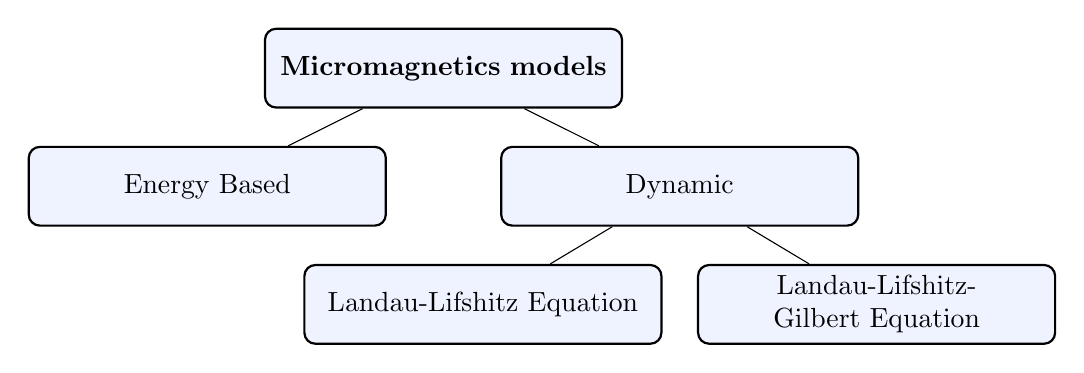
\begin{tikzpicture}[level 1/.style={sibling distance=6cm},
    level 2/.style={sibling distance=5cm}]
    \node[block] {\textbf{Micromagnetics models}}
    child {node[block] {Energy Based}}
    child {node[block] {Dynamic}
      child {node[block] {Landau-Lifshitz Equation}}
      child {node[block] {Landau-Lifshitz-Gilbert Equation}}
    };
  \end{tikzpicture}
  \caption{Possible approaches of a standard numerical micromagnetic model.}
  \label{fig:types-micromag-model}
\end{figure}


\subsection{Energy Based Micromagnetics}
\label{sec:energy-based-micr}

Energy based methods find an equilibrium state of the magnetic system by finding the minimum energy with respect to variation of $\Mv$. For example Fredkin and Koehler used a finite element energy minimisation method.\cite{Koehler1992} Energy based methods require less computational effort than dynamic methods. However they cannot give any information about the time evolution of a system.\cite{Fidler2000} This is an important problem in many areas: for example in magnetic data storage the time taken to reverse the magnetisation of a bit is of key interest.

% could include more details on how to search for minima.

\subsection{Dynamic Micromagnetics}
\label{sec:land-lifsch-gilb}

Dynamic micromagnetic methods model the time evolution of the magnetisation, for given effective field, as a differential equation. Starting with the quantum mechanical angular momentum of an electron, and converting from a single spin a continuous magnetisation gives\cite{Kronmuller2003}
\begin{equation}
  \label{eq:38}
  \dMdt = - \gymagc \Mv \times \Hv,
\end{equation}
where $\Hv$ is the total effective field
\begin{equation}
  \Hv = \Happ + \Hca + \Hex + \Hms.
  \label{eq:Heff}
\end{equation}
Equation~\eqref{eq:38} represents the procession of the magnetisation about the effective field, as shown in \autoref{fig:LLG-terms}. Other effective fields can be added to equation~\eqref{eq:Heff} to model other physical effects such as finite temperature or magnetostriction.

However equation~\eqref{eq:38} implies that the precession motion is undamped, \ie no energy is lost and the magnetisation continues to precess forever. This is obviously not the case so an empirical damping term is added:
\begin{equation}
  \label{eq:LL}
  \dMdt = - \gymagc \Mv \times \Hv - \frac{\dampc \gymagc}{M_s} \Big( \Mv \times (\Mv \times \Hv) \Big),
\end{equation}
where $\dampc$ is an experimentally determined material parameter related to the strength of the damping. Equation~\eqref{eq:LL} is referred to as the Landau-Lifshitz.\cite{Landau1935} The effects of the precession and damping terms are shown in \autoref{fig:LLG-terms}.

\begin{figure}[ht!]
  \centering
  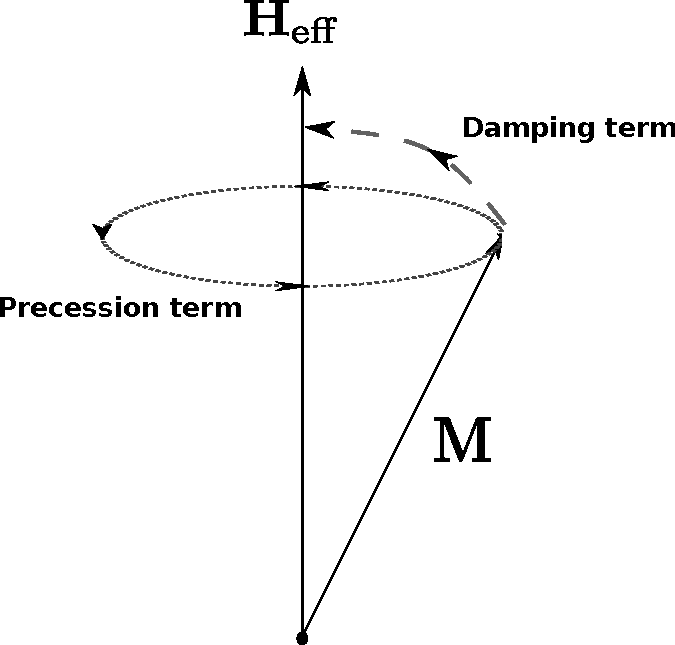
\includegraphics[width=0.6\textwidth]{./images/LLG-terms}
  \caption{The effects of the precession and damping terms in the Landau-Lifshitz and Landau-Lifshitz-Gilbert equations on the magnetisation direction, $\Mv$, of a single magnetic moment with a constant effective field
.}
  \label{fig:LLG-terms}
\end{figure}

However, there are still problems with this equation: for large damping the overall speed of the
motion increases without any increase in the precession speed. Hence the damping dominates and the switching time increases as damping is increased which is physically incorrect.\cite{Mallinson1987} There is another form of equation~\eqref{eq:LL} due to Gilbert\cite{Gilbert2004}, called the Landau-Lifshitz-Gilbert equation, which does not suffer from this problem
\begin{equation}
  \label{eq:Gilbert}
  \dMdt = - \gymagc \Mv \times \Hv + \frac{\dampc}{M_s} (\Mv \times \dMdt),
\end{equation}
where $\dampc \neq \dampc_L$. Equation~\eqref{eq:Gilbert} can be rearranged into the same form as equation~\eqref{eq:LL}, giving
\begin{equation}
  \label{eq:LLG}
  %\tag{LLG}
  \dMdt = \frac{-\gymagc}{1 + \dampc^2} \Big[ (\MxH) + \frac{\dampc}{M_s} \Big(\Mv \times (\MxH) \Big) \Big].
\end{equation}

Equations~\eqref{eq:LL}, \eqref{eq:Gilbert} and \eqref{eq:LLG} link the unknown magnetisation vector as a function of time $\Mv(t)$ with the effective field $\Hv$. To determine $\Mv$ at an arbitrary time $t \neq 0$ we need to integrate one of the above equations with respect to time. This is usually done numerically by employing a time discretisation method as discussed in \autoref{sec:time-discretisation}.

Note that there is no spatial dependence directly contained in equations~\eqref{eq:LL}, \eqref{eq:Gilbert} and \eqref{eq:LLG}. However the exchange effective field and magnetostatic field do contain spatial dependence, so usually the final equation to be solved after all substitutions really is a partial differential equation.

Examples of currently available micromagnetic models include the \texttt{OOMMF}\cite{oommf-website} and \texttt{nmag}\cite{Fischbacher2007} packages, which both use the dynamic method exclusively, along with \texttt{magpar}\cite{Scholz2003} and \texttt{FEMME}\cite{suessco-website} which can use either dynamic or energy based methods.


\subsubsection{Magnetisation boundary conditions}
\label{sec:magn-bound-cond}

The boundary condition on the magnetisation $\mv$ (in dimensional form) is \cite[pgs. 178, 181]{Aharoni1996}
\begin{equation}
  \Mv \times \bigb{ C \dMdn + \pd{w_s}{\Mv}} = \zerov,
\end{equation}
where $C$ is some exchange coeff ??ds and $w_s$ is the surface anisotropy.
Equivalently
\begin{equation}
    \Mv \times \dMdn = \frac{-1}{A} \Mv \times \pd{w_s}{\Mv}.
\end{equation}

For simplicity we commonly consider the case of zero surface anisotropy ($w_s \equiv 0$), in this case the boundary condition becomes
\begin{equation}
  \label{eq:llg-bc}
  \Mv \times \dMdn = \zerov.
\end{equation}
This condition can be arranged into a simpler form: we first note that for equation~\eqref{eq:llg-bc} to hold either $\Mv = \zerov$, $\dMdn = \zerov$ or $\Mv$ is parallel to $\dMdn$.
Clearly $\Mv$ is not the zero vector inside the ferromagnet.
Also we know that the magnetisation length does not change, so $\pd{\Mv}{\av} \cdot \Mv = 0$ for any direction $\av$ (since the change in magnetisation projected onto the magnetisation direction is the change in magnetisation length) hence $\Mv$ and $\dMdn$ cannot be parallel.
So the final boundary condition is simply
\begin{equation}
  \dMdn = \zerov.
\end{equation}


\section{Non-dimensionalisation}
\label{sec:normalisations-appendix}

% ??ds talk about why?

% no unecessary (for the maths) parameters
% improves accuracy by minimising round off error

\subsection{The Landau-Lifshitz-Gilbert equation}
\label{sec:land-lifsh-gilb-normalisation}

We start from the Landau-Lifshitz-Gilbert equation with the magnetostatic, applied, exchange and magnetocrystalline (effective) fields. 
\begin{align}
  \pd{\Mv^*}{t^*} &= - \gymagc \Mv^* \times \Hv^* + \frac{\alpha}{M_s} \Mv^* \times \pd{\Mv^*}{t^*}, \label{eqn:llgnd} \\
  \Hv^* &= \Happ^* - \nabla^* \phi^* + \frac{2\Exchc^*}{\mu_0 M_s} \nabla^{*2} \mv + \frac{2\Kone^*}{\mu_0 M_s} (\mv \cdot \ev) \ev,
          \label{eqn:effnd} \\
  \nabla^{*2} \phi^* &= \nabla^* \cdot \Mv^*, \label{eqn:phind}
\end{align}
where we use $^*$ to denote the dimensional variables, operators and constants that will be non-dimensionalised. We assume for simplicity that $M_s$, $\Exchc$ and $\Kone$ are all
constant throughout the magnetic materials used.

Let
\begin{equation}
  \label{eqn:nddefs}
  \begin{aligned}
    \Mv^* &= M_s \mv,  \\
    \phi^* &= \Phi \phi,  \\
    \Hv^* &= M_s \hv,  \\
    \Kone^* &= \nK \kone,  \\
    t^* &= \frac{1}{\gymagc M_s} t,  \\
    x_i^* &= l x_i. 
  \end{aligned}
\end{equation}
Note that $\Mv$ and $\Hv$ have the same units so we use the same normalisation factor. For dimensional purposes derivatives are equivalent to division by the variable differentiated with respect to, so $\nabla^* = \frac{1}{l} \nabla$, $\pd{a}{t^*} = \gymagc M_s \pd{a}{t}$ etc.

Combining equation~\eqref{eqn:llgnd} with the definitions~\eqref{eqn:nddefs} gives
\begin{equation}
  \notag
  \dmdt \gymagc M_s^2 =
  - \gymagc M_s^2 \mv \times \hv + \frac{\alpha}{M_s} \gymagc M_s^3 \mv \times \dmdt,
\end{equation}

cancelling the various constants results in the non-dimensionalised Landau-Lifshitz-Gilbert equation
\begin{equation}
  \label{eq:53}
  \dmdt = - (\mv \times \hv) + \alpha (\mv \times \dmdt).
\end{equation}

Similarly for equation~\eqref{eqn:phind}
\begin{align*}
  \frac{1}{l^2} \Phi \nabla^{2} \phi &= \frac{1}{l} M_s \nabla \cdot \mv, \\
  \frac{\Phi}{M_s l} \nabla^{2} \phi &= \nabla \cdot \mv.
\end{align*}

Letting $\Phi = M_s l$ we obtain
\begin{equation}
  \label{eq:57}
  \lap \phi = \nabla \cdot \mv.
\end{equation}

Repeating the substitutions for equation~\eqref{eqn:effnd} gives
\begin{align*}
  M_s \hv &= M_s \happ - \frac{\Phi}{l} \nabla \phi + \frac{2 \Exchc }{\mu_0 M_s} \frac{1}{l^2} \lap \mv + \frac{2\kone}{\mu_0 M_s}  \nK (\mv \cdot \ev) \ev, \\
  \hv &= \frac{M_s}{M_s} \happ - \frac{M_s}{M_s} \nabla \phi + \frac{2 \Exchc}{\mu_0 M_s^2} \frac{1}{l^2} \lap \mv + \frac{2\kone}{\mu_0 M_s^2} \nK (\mv \cdot \ev) \ev, \\
  \hv &= \happ - \nabla \phi + \frac{2 \Exchc}{\mu_0 M_s^2} \frac{1}{l^2} \lap \mv + \frac{2\kone}{\mu_0 M_s^2} \nK (\mv \cdot \ev) \ev, \\
\end{align*}

This can be further simplified by choosing the exchange length\footnote{There are actually two exchange lengths: one based on the strength of exchange as compared with the magnetostatic field and another by comparison with the magnetocrystalline anisotropy. We use the magnetostatic-field-based exchange length for normalisation to avoid division by zero in the case of zero magnetocrystalline anisotropy.} as the characteristic length scale
\begin{equation}
  \label{eqn:l-normalisation}
  l = \sqrt{ \frac{2 \Exchc}{\mu_0 M_s^2} },
\end{equation}

and
\begin{equation}
  \label{k-normalisation}
  \nK = \frac{ \mu_0 M_S^2}{2}.
\end{equation}

So the final system of equations is
\begin{equation}
  \begin{aligned}
    \dmdt &= - \mv \times \hv + \alpha \mv \times \dmdt, \\
    \hv &= \happ - \nabla \phi + \lap \mv + \kone (\mv \cdot \ev) \ev.
    \label{eqn:nd-llg-full}
  \end{aligned}
\end{equation}

\subsection{The Landau-Lifshitz form of the LLG}
\label{sec:land-lifsh-normalisation}

The dimensional Landau-Lifshitz equation is given in equation~\eqref{eq:LLG}:
\begin{equation}
  \label{eq:LLG-dim}
  (1 + \dampc^2) \pd{\Mv^*}{t^*} = - \gymagc \Mv^* \times \Hv^*
  - \frac{\gymagc \dampc}{M_s} \Mv^* \times (\Mv^* \times \Hv^*).
\end{equation}
The non-dimensionalisation process is essentially the same as for the Gilbert form, by substituting in the normalisations in equation~\eqref{eqn:nddefs} we obtain
\begin{equation}
  (1 + \dampc^2) \dmdt = - \mv \times \hv - \dampc \mv \times (\mv \times \hv).
\end{equation}
The field equations are obviously identical to those in equation~\eqref{eqn:nd-llg-full}.


Alternatively the time variable could be normalised differently to remove the factor of $(1 + \dampc^2)$ by using
\begin{equation}
  t^* = \frac{1 + \dampc^2}{\gymagc M_s} t.
\end{equation}
This results in
\begin{equation}
  \dmdt = -\mxh -\dampc \mxmxh.
\end{equation}
However this means that time scale changes when switching between the two forms, making comparisons more difficult.

\subsection{Boundary conditions}
\label{sec:non-dim-boundary-conditions}

The boundary conditions on the LLG are
\begin{equation}
  \Mv^* \times \pd{\Mv^*}{\nv*} = \frac{-1}{A} \Mv^* \times \pd{w_s^*}{\Mv^*}.
\end{equation}
Using the substitutions from above this becomes
\begin{equation}
  \begin{aligned}
    \frac{M_s^2}{l} \mv \times \dmdn &= \frac{-2}{l^2 M_s^2 \mu_0} \frac{M_s W}{M_s} \mv \times \pd{w_s}{\mv}, \\
    \mv \times \dmdn &= \frac{-2 W}{l \mu_0}  \mv \times \pd{w_s}{\mv}
  \end{aligned}
\end{equation}

??ds not sure what to do next, not important since no surface anisotropy for me...



\subsection{Energy}
\label{sec:energy-calculations}

Sometimes we may need to know the non-dimensional energy of a micromagnetic state in a form consistent with that used for the LLG equation. One example is for the computation of an effective damping constant, see section ??ds.

We repeat the process used in \autoref{sec:land-lifsh-gilb-normalisation} to get a set of non-dimensionalised energy equations, starting from the equations given in \autoref{sec:energy-magnetic-body}:

\begin{equation*}
  \Eapp^* = - \mu_0 \int_{\magd} \Mv^* \cdot \Happ^* \d \magd^*,
\end{equation*}
\begin{equation}
  \Ems^* =  \frac{-\mu_0}{2} \int_{\magd} \Mv^* \cdot \Hms^* \d \magd^*,
\end{equation}
\begin{equation*}
  \Eex^* =  \Exchc \int_{\magd} (\nabla^* \mv)^2 \d \magd^*,
\end{equation*}
\begin{equation*}
  \Eca^* =  -\Kone^* \int_\magd (\mv \cdot \ev)^2 \d \magd^*.
\end{equation*}

We substitute definitions~\eqref{eqn:nddefs}, \eqref{eqn:l-normalisation}, \eqref{k-normalisation} and $E^* = \nE e = \mu_0 M_s^2 l^d \, e$ where $d$ denotes the number of spatial dimensions:
\begin{equation*}
  \eapp = -\mu_0 M_s^2 l^d \frac{1}{\nE} \int_{\magd} \mv \cdot \happ \d \magd
  = - \int_{\magd} \mv \cdot \happ \d \magd,
\end{equation*}
\begin{equation}
  \ems = \frac{-\mu_0 M_s^2 l^d}{2} \frac{1}{\nE} \int_{\magd} \mv \cdot \hms \d \magd
  = -\frac{1}{2} \int_{\magd} \mv \cdot \hms \d \magd,
\end{equation}
\begin{equation*}
  \eex =  \frac{\mu_0 M_s^2 l^2}{2} \frac{l^d}{l^2} \frac{1}{\nE} \int_{\magd} (\nabla \mv)^2 \d \magd
  = \frac{1}{2} \int_{\magd} (\nabla \mv)^2 \d \magd,
\end{equation*}
\begin{equation*}
  \eca = - \frac{\mu_0 M_s^2}{2 } l^d \kone \frac{1}{\nE} \int_\magd (\mv \cdot \ev)^2 \d \magd
  = \frac{-\kone}{2} \int_\magd (\mv \cdot \ev)^2 \d \magd.
\end{equation*}
Note that we have used
\begin{equation}
  \d \magd^* = \d (x^*)^d = l^d \d x^d = l^d \d \magd.
\end{equation}


%%% Local Variables:
%%% mode: latex
%%% TeX-master: "./main"
%%% End:

\chapter{Numerical Methods for Dynamic Micromagnetic Modelling}
\label{sec:numer-meth-micr}

??ds In general should I cite models using each method?


In this Chapter we give an overview of numerical methods that have previously been used in dynamic micromagnetic calculations.
These calculations involve solving some form of the LLG equation \cref{eq:LLG} with effective fields determined by energy derivatives as discussed in \cref{sec:cont-micromag}.
These systems of partial differential equations (PDEs) can only be solved analytically in a few extremely simple cases\footnote{For example the Stoner-Wolfarth theory for the rotation of a single grain \cite{Stoner1948a}.} \cite{Aharoni1996}, so numerical solution methods are almost always necessary.

Many numerical methods for solving non-linear PDEs, such as \cref{eq:LLG}, can be thought of as a combination of various component methods, each of which handles a different part of the conversion from a continuous PDE into an algorithm which can be performed by a computer\footnote{Technically proofs of convergence etc. should be carried out for every different combination of time and space discretisation\cite[382]{Iserles2009}; in practice suprises seem to be rare, at least within micromagnetics.}.

The essential components of a numerical method for solving PDE problems are:
\begin{itemize}
\item Spatial discretisation: convert space derivatives into algebraic relationships between discrete points in space, \eg finite elements, finite differences, macrospin models. 
\item Time discretisation (a.k.a. time integration):  convert time derivatives into algebraic relationships between points in time, \eg Runge-Kutta methods, backwards difference formulae.
\end{itemize}
For some choices of time and space discretisations additional component methods are needed:
\begin{itemize}
\item Linearisation procedure: Solve a system of non-linear algebraic equations, often by an iterative procedure which requires the solution of a sequence of systems of linear algebraic equations, \eg Newton-Raphson method, Picard/fixed-point iteration. 
\item Linear solver: solve a system of linear algebraic equations, \eg LU decomposition, Krylov solvers, multigrid methods. 
\end{itemize}

Additionally in micromagnetic modelling the calculation of the magnetostatic field is required.
If the integral form given in \cref{eq:Hmsint} is used then an additional integral evaluation method is needed to handle it.
Alternatively, if the equivalent potential formulation \cref{eq:Hms}, \cref{eq:cont-phi-bound} is used then the magnetostatic field calculation simply requires solving additional PDEs.

It should be noted that not all methods fit into this framework of applying separate methods for each part of the problem, see \cref{sec:advanced-lin} for one example.


\section{Spatial Discretisation}
\label{sec:spat-discr}

\subsection{Macrospins}
\label{sec:sd-macrospins}

In a granular magnetic material (a material consisting of magnetic grains separated by a non-magnetic material) the simplest way to handle spatial variation in the problem is to assume that within each grain the exchange effective field is so strong that the magnetisation is constant, \ie that each grain behaves as a single \emph{macrospin}.
We assign a single value of $\Mv$ to each macrospin and proceed to calculate energy, effective field and/or magnetisation of each macrospin as required.
One caveat is that the effects of the magnetostatic field of a grain on the grain itself is not automatically accounted for since there is no modelling of intra-grain effects.
Hence it must be calculated and included separately to the magnetostatic interactions between grains.
When included in this way the magnetostatic self field is often called the \emph{shape anisotropy} since it is dependent on the shape of the grain and acts in a similar way to the magnetocrystalline anisotropy. 

This macrospin approach may be used with any system in which there are a number of ``small'',\footnote{All dimensions of the bodies must be much smaller than the exchange length so that all magnetisation within the body is approximately parallel.} separate magnetic bodies with approximately uniform magnetisation inside the body.

The obvious downside of a macrospin approach is that it only applies to a fairly specific geometry, although the case of a granular media has been of much interest for magnetic data storage. 
Additionally, if there are non-uniformities in magnetisation within the regions where it has been assumed constant the model may be inaccurate.

However it is often simpler to construct a macrospin model than to use the more general methods described in \crefs{sec:sd-finite-diff-meth, sec:sd-finite-elem-meth}.
Also the assumption that each grain has uniform magnetisation will reduce the number of calculations needed.

Closely related to macrospin models are atomistic models \cite{Evans2014}.
In these models the assumption of a continuous magnetisation $\mv(\xv, t)$ is dropped in favor of an assumption that each atom is the location of a single macrospin.
As such they allow modelling of some systems, such as antiferromagnetic materials, that are inaccessible using micromagnetics.
However, the required spatial resolution comes with a large increase in computational cost.


\subsection{Finite Difference Methods}
\label{sec:sd-finite-diff-meth}

Another method of spatial discretisation is the finite difference method: a single magnetisation vector is assigned to each point on (or ``cell'' in) a simple square/cubic grid which covers the entire domain.
Spatial derivatives in the PDE are then approximated by using truncated Taylor series expansions.

The finite difference method works well for very simple geometries when the grid can be lined up with all geometric features.
For example when we are interested in how the magnetisation evolves over time in a non-granular cuboid-shaped thin film of magnetic material a finite difference method will be sufficient (\eg in the $\mu$mag standard problems \cite{mumag-website}).

However when the geometry involves curves, diagonals, hexagonal grains, bit patterned media or any other more complex geometric system other methods are better suited.


\subsection{Finite Element Methods}
\label{sec:sd-finite-elem-meth}

A more complex method of spatial discretisation is the finite element method \cite{HowardElmanDavidSilvester2006}.
Here the magnetic body is divided up into a finite number of non-overlapping polygonal \emph{elements}, which can vary in both size and shape.
Within each of these elements each magnetisation component is approximated by a simple polynomial function of space, typically a linear polynomial.
Spatial derivatives are calculated by simply differentiating these polynomial functions.
More details of the finite element method are given in \cref{sec:intr-finite-ele-diff}.

The main advantage of the finite element method is that it can accurately approximate any geometrical feature by an appropriate arrangement of the polygonal elements.
An additional advantage is that the size of elements (and thus the accuracy of the approximation) can be varied arbitrarily as needed to give better accuracy in more complex or important regions. 
The choice of element size can be done automatically using \emph{adaptive mesh refinement}: after each calculation an error estimate is calculated (known as \emph{a posteriori} error estimation).
If the error is determined to be too high anywhere the mesh is refined near that region and the calculation is repeated.
Hence, given the desired error and a method to estimate the error, a mesh giving an efficient and accurate approximation can be automatically generated \cite{Schrefl1999}.

The major downside of finite element models is that the underlying mathematics is more complex than that required for other methods, especially finite difference methods.
Also the set up time and memory usage can be greater because of the additional ``bookkeeping'' required to keep track of the more complex meshes.


\section{Time Integration}
\label{sec:time-discretisation}

Time integration schemes are used to convert the time derivatives of a PDE into a form that can be handled computationally. 
When discussing time integration schemes it is helpful to use a (vector) initial value ordinary differential equation as an example:
\begin{equation}
  \begin{aligned}
    \frac{d \yv}{dt} &= \ffv{t, \yv}, \\
    \yv(0) &= \yv_0,
    \label{eq:45}
  \end{aligned}
\end{equation}
where $\fv(t,\yv)$ is a known function and $\yv_0$ is the (known) initial condition.
After the application of one of the spatial discretisations described above a PDE is typically reduced to the form \cref{eq:45}, this sometimes is called a \emph{semi-discretised} PDE.

The time integration methods discussed here all bear a strong similarity to the finite difference method discussed in \cref{sec:sd-finite-diff-meth}, except that the independant variable discretised is time instead of space.
This is appropriate since time is one-dimesional, hence no complex geometry is possible and so typically there is no need for the more advanced finite element method.

Some key attributes of a time integration scheme are \cite{Atkinson2009}:
\begin{itemize}
\item \textbf{Accuracy (order)} -- An estimate of how rapidly the approximate solution converges as the time step size is reduced.

\item \textbf{Stability} -- Roughly speaking a scheme is stable if the approximate solution does not ``blow up'' (\ie become catastophically inaccurate, infinite, oscillate in non-physical ways, \ldots) for sufficiently large time steps (see \cref{sec:A-stability} for a more rigorous description).

\item \textbf{Conservation properties} -- Some differential equations have properties which should ideally be conserved in the discretised system.
For example, certain important properties of the Landau-Lifshitz-Gilbert equation discussed in \cref{sec:prop-cont-llg}.
Schemes which conserve such properties are often referred to as ``geometric'' integrators.

\item \textbf{Self-starting} -- A scheme is self starting if it only requires a single initial value.
This is desirable because methods of estimating additional initial values make the final scheme more complex and may introduce additional errors.
\end{itemize}

These attributes are discussed more rigorously in the rest of this section.

\subsection{Explicit and implicit time integration schemes}
\label{sec:explicit-vs-implicit-schemes}

Explicit time discretisation schemes calculate the value at the next time step in terms of the value(s) at the present and/or previous time steps.
The simplest such scheme is the \emph{(forward) Euler method}
\begin{equation}
  \label{eq:44}
  \yv_{n+1} = \yv_n + \dtn f(t_n, \yv_n),
\end{equation}
where $\dtn = t_{n+1} - t_n$ is the $n$-th time step size and $\yv_i$ is the approximation to $\yv(t_i)$.
Clearly, given $f(t,y)$ and an initial value for $y(t_0)$ we can solve for $y(t_n)$ for any $n$.

In contrast to explicit schemes, implicit schemes use the value at the next time step in its own calculation.
Hence at each step a (possibly non-linear) system of equations must be solved.
The simplest implicit scheme is the \emph{backward Euler method} (BDF1)
\begin{equation}
  \label{eq:bdf1-definition}
  \yv_{n+1} = \yv_n + \dtn \ffv{t_{n+1}, \yv_{n+1}}.
\end{equation}

At first glance it seems that the additional solution of a system of equations required for a step of an implicit scheme mean would that explicit schemes are more efficent, and it is true that one step of an implicit method requires more computational effort than a step of an explicit method.
However all explicit time integration schemes suffer from issues of limited stability for some problems, and so are forced to use time step sizes much smaller than would be required for reasons of accuracy (see \cref{sec:A-stability} for details).
In these cases implicit schemes can be much more efficient, problems where this is the case are often called ``stiff'' problems.
The semi-discretisation of a PDE often results in a stiff problem.
In \cref{cha:stiffn-llg-equat} we investigate stiffness in micromagnetics problems.


% Micromagnetics solvers for non-stiff systems commonly use the RK4 (fourth order Runge-Katta) method \cite{Suess2002}.
% Micromagnetics models commonly use BDF schemes of various order \cite{Suess2002} or the implicit midpoint rule \cite{DAquino2005} for the modelling of stiff systems.


\subsection{Some implicit time integration schemes}
\label{sec:some-implicit-time-integrators}

For the remainder of this section we will use three time integration schemes with good stability and accuracy properties that are widely employed in practice as examples.
All three are implicit schemes for reasons of stability, as mentioned in \cref{sec:explicit-vs-implicit-schemes}.

\emph{Trapezoid rule} (TR) is the average of the forward and backward Euler methods from \cref{sec:explicit-vs-implicit-schemes}:
\begin{equation}
  \yv_{n+1} = \dtn (\ffv{t_{n+1}, \yv_{n+1}} + \ffv{t_n, \yv_n})/2.
  \label{eq:tr-definition}
\end{equation}

The \emph{second order backwards difference formula} (BDF2) is:
\begin{equation}
  \frac{\yv_{n+1} - \yv_n}{\dtn} = \frac{\dtn}{2\dtn + \dtx{n-1}} \frac{\yv_n - \yv_{n-1}}{\dtx{n-1}} 
  + \frac{\dtn + \dtx{n-1}}{2\dtn + \dtx{n-1}} \fv(t_{n+1}, \yv_{n+1}).
\end{equation}

The method that this thesis focuses on (for reasons that will become clear through the remainder of this section) is the \emph{implicit midpoint rule} (IMR).
It is given by:
\begin{equation}
  \label{eq:imr-definition}
  \yv_{n+1} = \yv_n + \dtn \ffv{\frac{t_{n+1} + t_n}{2}, \frac{\yv_n + \yv_{n+1}}{2}}.
\end{equation}
Note that for cases where $\fv$ is linear in both $t$ and $\yv$ IMR, \cref{eq:imr-definition}, is equvalent to TR, \cref{eq:tr-definition}.
In general the properties of the two methods are similar.

IMR is trivial to implement in any existing implicit solver: take a step of BDF1, \cref{eq:bdf1-definition}, using $\dtn^\bdfo = \dtn^\imr/2$ then update via
\begin{equation}
  \begin{aligned}
    t_{n+1} &\rightarrow t_{n+1} + \dtn^\imr/2, \\
    \mv_{n+1} &\rightarrow 2\mv_{n+1} - \mv_n.
  \end{aligned}
\end{equation}
This is exactly equivalent to IMR with a step size of $2\dtn$ \cite{Malidi2005}.

TR and IMR are both self starting, while BDF2 requires an additional startup value.
This can be generated, for example, by taking a single step of IMR or TR before beginning the use of BDF2.


\subsection{Local truncation error and order}
\label{sec:deriv-local-trunc}

The \emph{local truncation error} (LTE) of a time integration scheme is the error due to a single integration step.
It can be calculated by substituting $\yv_n = \yv(t_n)$, $\yv_{n-1} = \yv(t_{n-1})$, etc. into the approximation for the next time-step, then subtracting the result from the exact solution at the next time-step, $\yv(t_{n+1})$, \ie
\begin{equation}
  \label{eq:60}
  \lte = \yv(t_{n+1}) - \hat{\yv}_{n+1},
\end{equation}
where the history values ($\yv_{n}, \yv_{n-1}, \ldots$) used to calculate $\hat{\yv}_{n+1}$ are exact.
For example the local truncation error of IMR is
\begin{equation}
  \lte^\imr =  \yv(t_{n+1}) - \yv(t_n) - \dtn \ffv{\thf, \frac{\yv(t_n) + \yv_{n+1}^\imr}{2}}.
  \label{eq:trunc-start}
\end{equation}

If the local truncation error of a time integration scheme is such that 
\begin{equation}
  \lte \leq c \dtn^p
\end{equation}
then we say that the scheme is of order $p$.

It is important to distinguish the local truncation error from the \emph{global (temporal) error}
\begin{equation}
  \label{eq:global-temporal-error}
    E_n = \yv(t_{n+1}) - \yv_{n+1}.
\end{equation}
The difference is that the global error includes any error accumulated over previous time steps (\ie the exact values $\yv(t_n)$ in \cref{eq:60} are replaced by their approximations).
Note that because of this accumulation the global error will typically be larger than the LTE.
For example the global error of IMR expressed in the same form as \cref{eq:trunc-start} is
\begin{equation}
  E_n^\imr =  \yv(t_{n+1}) - \yv_n^\imr - \dtn \ffv{ \thf, \frac{\yv_n^\imr + \yv_{n+1}^\imr}{2} }.
\end{equation}

We now give a derivation of the local truncation error of IMR. 
The derivations for TR and BDF2 are much simpler and can be found in most text books on the subject.
We first write the Taylor expansion $\yv(t_{n+1})$ and $\yv(t_{n})$ about $\thf$.
We use the midpoint rather than one of the end points (a typical choice in such calculations) because it results in simpler expressions.
Assuming that $\yv(t)$ is ``sufficiently smooth'' for the required derivatives to exist, its Taylor series expansion at $t_{n+1}$ about $\thf$ is given by
\begin{equation}
  \yv(t_{n+1}) = \yv(\thf + \frac{\dtn}{2}) = \yvhf + \frac{\dtn}{2} \yvhf['] 
  + \frac{\dtn^2}{8} \yvhf['']
  + \frac{\dtn^3}{48} \yvhf[''']
  + \order{\dtn^4}.
  \label{eq:taylornp1}
\end{equation}
Similarly, the expansion at $t_n$ about $\thf$ is
\begin{equation}
  \yv(t_n) = \yv(\thf - \frac{\dtn}{2}) = \yvhf - \frac{\dtn}{2} \yvhf['] 
  + \frac{\dtn^2}{8} \yvhf[''] 
  - \frac{\dtn^3}{48} \yvhf['''] 
  + \order{\dtn^4}.
  \label{eq:taylorn}
\end{equation}
Substituting \cref{eq:taylornp1} and \cref{eq:taylorn} into \cref{eq:trunc-start} gives\footnote{If we had chosen to Taylor expand about $t_n$ there would be an additional term in $\yv_n''$ in \cref{eq:trunc-mid}.}
\begin{equation}
  \lte^\imr = \underbrace{\frac{\dtn^3}{24} \yvhf[''']}_{\text{I}}
  + \underbrace{\dtn\bigs{ \yvhf['] - \ffv{\thf, \frac{\yv(t_n) + \yv_{n+1}}{2}} }}_{\text{II}}
  + \order{\dtn^4}.
  \label{eq:trunc-mid}
\end{equation}

There are two parts to \cref{eq:trunc-mid}: the first term (I) is fairly standard for second order time integration schemes (see \eg \cref{cha:trunc-errors}).
The second term (II) originates from the use of an approximation to $\yv(\thf)$ in the evaluation of $\fv$ (\ie the Runge-Kutta nature of IMR).
The rest of the derivation requires applying Taylor expansions to II and is carried out in \cref{sec:full-imr-lte-calculation}.
The final result shows that IMR is of second order:
\begin{equation}
  \lte^\imr = \frac{\dtn^3}{24} \left[\yvhf['''] - 3 \dfdyhf \cdot \yvhf[''] \right]
  + \order{\dtn^4},
  \label{eq:trunc-final}
\end{equation}
where $\dfdyhf = \pd{\fv}{\yv}\evalat{t=\thf}$ is the Jacobian of $\fv$ with respect to $\yv$ evaluated at $t=\thf$.
An additional condition required in the derivation is that ??ds the magnitude of the eigenvalues of $\dtn\dfdyhf$ are less than one, the implications of this are discussed in \cref{sec:order-reduction}.

The TR \cite[261]{GreshoSani} and BDF2 \cite[715]{GreshoSani} methods are also second order.
Their local truncation errors are similar to term I of \cref{eq:trunc-mid}:
\begin{equation}
  \label{eq:tr-lte}
  \lte^\tr = \yv_{n+1} - \yv(t_{n+1}) = -\frac{\dtn^3 \yv_n'''}{12}
  + \order{\dtn^4},
\end{equation}
and
\begin{equation}
  \label{eq:bdf2-lte}
  \lte^\bdf = \yv_{n+1} - \yv(t_{n+1}) = \frac{(\dtn + \dtx{n-1})^2}{\dtn(2\dtn + \dtx{n-1})}
  \frac{\dtn^3 \yv_n'''}{6}
  + \order{\dtn^4}.
\end{equation}


\subsection{A-stability}
\label{sec:A-stability}

To discuss the stability of time integrators the following test equation is widely used
\begin{equation}
  \ffv{\yv} = \lambda \yv,
  \label{eq:ode-test-f}
\end{equation}
\ie
\begin{equation}
  \yv(t) = \exp(\lambda t).
\end{equation}

A-stablility\footnote{The A does not stand for anything, it is just ``A''\cite[40]{HairerWanner}, in particular it does \emph{not} mean ``absolute stability''.} is the property that a method is has no stability restrictions on the time step size when used to integrate \cref{eq:ode-test-f} for all $\lambda$ with $\realp(\lambda) \leq 0$.
When $\realp(\lambda) > 0$ the ODE itself is unstable and so stability is not expected in general.
A-stability is a good way to classify the suitability of a time integrator for solving ``stiff'' ODEs.
Such ODEs often emerge from the semi-discretisation of a PDE.

The IMR, TR, BDF1 and BDF2 methods are all A-stable \cite[pgs. 43, 251]{HairerWanner}.
Linear explicit methods are never A-stable \cite{Nevanlinna1974} (``linear'' methods in this reference include all common time integration methods: Runge-Kutta, multistep, predictor-corrector, \ldots)\footnote{These limitations could theoretically be circumvented by using significantly more complex methods, but such questions are far beyond the scope of this thesis.}, which is the main reason for our focus on implicit methods.
Additionally there are no A-stable linear multistep methods\footnote{A-stable implicit Runge-Kutta methods of higher order do exist, see \eg \cite[73]{HairerWanner}.
However moving to higher order methods significantly increases the size of the system to be solved at each step. Hence they are prohibatively expensive for the time integration of semi-discretised PDEs.
Also second order is in some sense ``good enough'' for LLG integration since the spatial accuracy is only second order and contains higher order derivatives than in time.
??ds talk to Milan/Matthias about this: it seems that with good preconditioning we can have \eg a 4th order method (Gauss order 4, higher order version of IMR) for only ~4x the cost per step, a gain of 25x in (computation time)/accuracy with steps of ~0.1} of order greater than 2 \cite[261]{GreshoSani}, which is why we have chosen the three widely used second order methods for discussion.

\subsection{Spurious numerical damping}
\label{sec:numerical-damping}

Some time integration methods create additional, non-physical damping in approximate solutions, even when none exists in the exact solution.
This is problematic for the modelling of highly oscillatory ODEs, such as the LLG with low damping.

We say that a time integration method causes spurious damping if when solving the test ODE \cref{eq:ode-test-f} with $\lambda = i\omega$ the magnitude of $y$ decreases over time.

For example, for the implicit midpoint rule:
\begin{equation}
  \begin{aligned}
    y_{n+1} &= y_n + \dtn i \omega (y_n + y_{n+1})/2, \\
    &= \frac{1 + i\dtn \omega/2}{1 - i\dtn \omega/2} y_n,
  \end{aligned}
\end{equation}
and so
\begin{equation}
  \begin{aligned}
    \abs{y_{n+1}}^2 &=  \frac{\abs{1 + i\dtn \omega/2}^2}{\abs{1 - i\dtn \omega/2}^2} \abs{y_n}^2, \\
    \abs{y_{n+1}}^2 &=  \frac{(1 + i\dtn \omega/2)(1 - i\dtn \omega/2)}
    {(1 - i\dtn \omega/2)(1 + i\dtn \omega/2)} \abs{y_n}^2, \\
    &=  \abs{y_n}^2.
  \end{aligned}
\end{equation}
So IMR does not cause spurious damping.

Since $f$ is linear in $y$ for this example ODE TR and IMR are identical
\begin{equation}
  \begin{aligned}
    y_{n+1} &= y_n + \dtn(i\omega y_n + i\omega y_{n+1})/2, \\
    &= y_n + \dtn i \omega (y_n + y_{n+1})/2.
  \end{aligned} 
\end{equation}
Hence the same property applies for TR.

For BDF1
\begin{equation}
  \begin{aligned}
    y_{n+1} &= y_n + \dtn i \omega y_{n+1}, \\
    &= \frac{1}{1 - i \dtn \omega} y_n.
  \end{aligned}
\end{equation}
Hence
\begin{equation}
  \begin{aligned}
    \abs{y_{n+1}} &= \sqrt{ \frac{1}{(1 - i \dtn \omega)(1 + i \dtn \omega)}} \abs{y_n}, \\
    &= \frac{1}{\sqrt{1 + \dtn^2 \omega^2}} \abs{y_n}, \\
  \end{aligned}
\end{equation}
and so the magnitude of $y$ decreases over time--the solution is damped.
The analysis for the second order BDF2 case is more complex due to the fact that it is a multistep method, but the result is the same: the solution suffers from non-physical damping \cite[265]{GreshoSani}.


\subsection{B-convergence and order reduction}
\label{sec:order-reduction}

It is known that certain implicit Runge-Kutta methods are susceptible to reduced accuracy when used to solve certain extremely stiff problems \cite[156]{Atkinson1994}\cite[225]{HairerWanner}.
In the case of the implicit midpoint rule this corresponds to the case when the error due to term II of \cref{eq:trunc-mid} is large. This occurs when $\pd{\fv}{\yv}\evalat{\thf{}}$ is large, \ie when the error in $\ffv{t, \yv}$ due to a small error in $\yv$ is large.

The concept of ``B-convergence'' is used to analyse this effect.
Roughly speaking a Runge-Kutta method is B-convergent of order $r$ if the global error is  $\order{\dtx{\text{max}}^r}$ for all sufficiently smooth ODEs without any assumption about the size of $\pd{\fv}{\yv}$.
The implicit midpoint rule is B-convergent of order 1 \cite[231]{HairerWanner}\footnote{In this reference IMR is refered to as the second order Gauss method, BDF1 is Radau IIA, TR is Lobatto IIIA \cite[72-76]{HairerWanner}.}, one order less than for typical ODEs.
In contrast, the TR and BDF methods do not suffer from order reduction \cite[159]{Atkinson1994}.
This is because all evaluations of $\fv$ are at integer time points (\ie $t_{n+1}, t_{n}, t_{n-1}, \ldots$ rather than $\thf$).

A simple test ODE gives a useful example of this phenomenon \cite[157]{Atkinson2009}
\begin{equation}
  \label{eqn:imr-test-order-reduction}
  \begin{aligned}
    f(t, y) &= -\lambda (y - g(t)) + g'(t), \\
    y(t) &= g(t), \\
  \end{aligned}
\end{equation}
for some function $g(t)$ and parameter $\lambda \geq 0$.
Note that $\pd{f}{y} = \lambda$, so we can directly control the second term of the IMR truncation error.

We now derive the LTE for IMR in this example when $\abs{\lambda\dtn} >> 1$.
From \cref{sec:full-imr-lte-calculation}, \cref{eq:trunc-implicit-form} we have that
\begin{equation}
  \begin{aligned}
    (1 + \frac{\dtn \lambda}{2})\lte^\imr &= \frac{\dtn^3}{24}
    \bigs{g'''(\thf) - 3 \lambda g''(\thf)} + \order{\dtn^4}, \\ 
  \end{aligned}
\end{equation}
Then using $\abs{\lambda\dtn} >> 1$:
\begin{equation}
  \begin{aligned}
    \frac{\dtn \lambda}{2} \lte^\imr &= \frac{\dtn^3}{24}
    \bigs{g'''(\thf) - 3 \lambda g''(\thf)} + \order{\dtn^4}, \\ 
    \lte^\imr &= \frac{\dtn^2}{12\lambda} \left[g'''(\thf) - 3 \lambda g''(\thf) \right] + \order{\dtn^4}.
  \end{aligned}
\end{equation}
So we can see that the order has been reduced by a factor of $1/\dtn$.
If addtionally $\abs{\lambda\dtn} >> \abs{g'''(t)}$, which will typically be true for very large $\lambda$ and $g \neq g(\lambda)$:
\begin{equation}
  \lte^\imr = \frac{-\dtn^2}{4} g''(\thf).
  \label{eq:reduced-order-imr-truncation-error}
\end{equation}


\subsection{Adaptivity}
\label{sec:adaptivity}

Adaptive time integration methods automatically select time step sizes in response to an estimate of the local truncation error.
This can improve efficiency depending on the equation being solved, for example on problems where a high frequency part of the solution is gradually damped out the time step can increase by orders of magnitude at later times without loss of accuracy.
Adaptive integration also greatly simplifies the use of the simulation program--the user only has to choose the allowed error and the program will handle the rest.

Most local truncation error estimators for implicit integrators (e.g. TR, BDF2) use a Milne-device based method \cite[707-716]{GreshoSani}.
This means that they compute an explicit estimate $\yv^E_{n+1} \sim \yv(t_{n+1})$  (sometimes known as a predictor step) to the same order of accuracy as the implicit method and using the same input values and derivatives.
They then use algebraic rearrangements of the local truncation error expressions of the predictor step and the implicit step to give an approximation of the true local truncation error.

No such estimation is possible for IMR because of the specific form of the local truncation error.
The details of this issue and the first (to the author's knowledge) algorithm for adaptive time integration with IMR are described in \cref{sec:adaptive-imr}.

It is also possible to create less general adaptivity methods based on error estimates specific to the equation being solved.
For example in cases where the damping is not exactly correct the effective damping can be used as an error estimator, as proposed by Albuquerque \etal \cite{Albuquerque2001}.
The disadvantage of this method (aside from the obvious requirement that the damping be inexact) is that, depending on the discretisation used, the error estimator may be unable to distinguish between insufficient space refinement and insufficient time refinement.
In particular this is the case when the solution is not completely divided into separate effective field calculations and pointwise time integration, such as in a typical Galerkin finite element model.

Additionally time error estimates for the LLG with limited effective field terms and a specific finite element discretisation were proven and used to perform adaptive time integration with both IMR and BDF2 by Banas \cite{Banas-thesis}.
??ds do these work, why does no one use them?
These estimates have the obvious limitation that they are only (directly) applicable to the case for which they were derived.
It is also a fairly complex derivation (at least for non-numerical analysts), and difficult to test because of its limited applicability.


\subsection{Magnetisation length conservation}
\label{sec:ensuring-constant-mv}

As discussed in \cref{sec:prop-cont-llg} the length of the magnetisation at a point does not change over time.
However in the approximations given by numerical methods this is often lost, and must be enforced separately.

A simple method of dealing with the constraint is to re-normalise $\Mv$ after some number of time steps or when the error in $|\Mv|$ exceeds some tolerance \cite{Fidler2000}.
However this approach fundamentally changes the system of equations being solved in a non-linear and unpredictable manner \cite{Lewis2003}.

??Ds rewrite:
If we have a system with only a single (macro)spin (\ie a single value of $\Mv$ represents the magnetisation of the entire system) it is easy to avoid this problem by using a spherical polar coordinate system $(r,\theta,\phi)$.
Equation~\cref{eq:LLG} can be expressed in terms of only the angles $(\theta,\phi)$ representing the direction of $\Mv$ and the non-convex constraint is automatically enforced since
\begin{equation}
  \label{eq:40}
  \pd{\abs{\Mv}}{t} = \pd{r}{t} \equiv 0.
\end{equation}
However to extend this to systems where $\Mv$ varies with space we have to use a separate spherical polar coordinate system at each point where $\dMdt$ is calculated.
Also a Cartesian global coordinate system is still needed to calculate the interactions between the discretised points (\ie magnetostatics, exchange coupling).
Hence we have to convert back and forth between coordinate systems during the simulation \cite{Scholz2003}.
Finally problems can occur with this approach as the polar angle, $\theta$, approaches zero because $\pd{\Mv}{t} \propto \frac{1}{\sin(\theta)}$ \cite{Fukushima2005}.

Geometric integration schemes aim to solve this problem by constructing a time integration scheme that naturally preserves the value of $|M_s|$.
Some examples of such schemes are based on IMR \cite{DAquino2005}, or a semi-explicit extension of IMR using explicit extrapolations of the effective field \cite{Spargo2003} \cite{Serpico2001}.
Alternatively geometric integration methods based on Cayley transforms can be used \cite{Lewis2003} \cite{Bottauscio2011}.


\subsubsection{Proof of magnetisation length conservation for IMR on the ODE LLG}
\label{sec:proof-magn-length-ode-imr-llg}

In this section we show that the discrete form of the Landau-Lifshitz-Gilbert equation that results from the use of the implicit midpoint rule maintains the magnetisation length conservation property of the continuous form shown in \cref{sec:prop-cont-llg}.
These results are applicable to cases where, after any spatial discretisation, each spatial point is time evolved by simply integrating the LLG with the values for that point, \ie finite difference and macrospin discretisations (but not finite elements).
For the purposes of this section we assume that the linearisation method is exact, \ie the discretised but non-linear Landau-Lifshitz-Gilbert equation is satisfied exactly.

As can be seen from \cref{eq:imr-definition} the IMR is defined by the following substitutions:
\begin{equation}
\begin{aligned}
  \label{eq:55}
  \pd{\mv}{t} &\rightarrow \frac{\mv_{n+1} - \mv_n}{\dtn}, \\
  \mv &\rightarrow \frac{\mv_{n+1} + \mv_n}{2}, \\
  t &\rightarrow \frac{t_{n+1} + t_n}{2}.
\end{aligned}
\end{equation}
So the IMR-discretised LLG is
\begin{equation}
  \frac{\mv_{n+1} - \mv_n}{\dtn} = - \frac{\mv_{n+1} + \mv_n}{2} \times
  \left(
    \hv \left[\frac{\mv_{n+1} + \mv_n}{2} \right]
    + \happ\left(\frac{t_{n+1} + t_n}{2}\right)
    - \dampc \frac{\mv_{n+1} - \mv_n}{\dtn}
  \right).
  \label{eqn:disc-llg}
\end{equation}

Intuitively the conservation properties of the IMR discretisation can be seen to come from the cancellation of cross terms in $\ip{\lop[\mv]}{\dmdt}$ for any symmetrical linear operator $\lop$.
More precisely:
\begin{equation}
  \begin{aligned}
    \label{eqn:imr-linop}
    \ip{\lop \left[ \frac{\mv_{n+1} + \mv_n}{2} \right]}{ \frac{\mv_{n+1} - \mv_n}{\dtn} }
    &= \frac{1}{2\dtn} \Big[
    \ip{\mv_{n+1}}{\lop \mv_{n+1}} + \ip{\mv_{n+1}}{\lop \mv_{n}} \\
    & \qquad\qquad - \ip{\mv_{n}}{\lop \mv_{n+1}} - \ip{\mv_{n}}{\lop \mv_{n}}
    \Big] \\
    &= \frac{1}{2\dtn} \Big[
    \ip{\mv_{n+1}}{\lop \mv_{n+1}}
    - \ip{\mv_{n}}{\lop \mv_{n}}
    \Big].
  \end{aligned}
\end{equation}
This means that any orthogonality relationships between $\lop \mv$ and $\dmdt$ in the continuous case carry over to the discrete case. ??ds more detail on what this means

We can now examine the change in magnetisation length using the same technique as in \cref{sec:prop-cont-llg}: take the dot product with $\frac{\mv_{n+1} + \mv_n}{2}$ on both sides of~\cref{eqn:disc-llg} and use the triple product identity \cref{eq:dot-cross-id} to get
\begin{equation}
  \label{eq:63}
  \frac{\mv_{n+1} + \mv_n}{2} \cdot \frac{\mv_{n+1} - \mv_n}{\dtn} = 0.
\end{equation}
Now using~\cref{eqn:imr-linop} with $\lop$ as the identity operator gives us
\begin{equation}
  \frac{\ip{\mv_{n+1}}{\mv_{n+1}} - \ip{\mv_n}{\mv_n} }{2 \dtn} = 0.
\end{equation}
Therefore
\begin{equation}
  \abs{\mv_{n+1}} = \abs{\mv_n},
\end{equation}
\ie the magnetisation length does not change between time steps.


Note that for other time integration schemes the property \cref{eqn:imr-linop} typically does not hold.
For example in the case of BDF1 we have
\begin{equation}
  \begin{aligned}
    \ip{\lop \bigs{\mv_{n+1}}}{ \frac{\mv_{n+1} - \mv_n}{\dtn} }
    &= \frac{1}{\dtn} \bigs{ \ip{\mv_{n+1}}{\lop \mv_{n+1}} 
      - \ip{\mv_{n+1}}{\lop \mv_n} }, \\
    &\neq \frac{1}{\dtn} \bigs{ \ip{\mv_{n+1}}{\lop \mv_{n+1}}
      - \ip{\mv_n}{\lop \mv_n} },
  \end{aligned}
\end{equation}
so orthogonality properties from the continuous form do not carry over in general.

Also note that the derivation of \cref{eq:63} only requires that the midpoint representation of magnetisation be used for terms directly in the llg, it does not require anything about the effective field calcuation.
This explains why the semi-explicit modification to IMR also conserves the magnetisation length. 


\subsection{Energy conservation/decay}
\label{sec:energy-cons}

Another geometrical property of the Landau-Lifshitz-Gilbert equation, also discussed in \cref{sec:prop-cont-llg}, is the conservation or controlled decay of energy depending on the value of the damping constant $\dampc$.

IMR also conserves energy when the damping term is zero and it ensures that the energy is a decreasing function of time when the damping is non-zero \cite{DAquino2005}.
The other geometric integration schemes mentioned in \cref{sec:ensuring-constant-mv}, in particular the semi-explicit modifications of IMR, do not have this property.


\subsubsection{Proof of energy property for IMR on the ODE LLG}
\label{sec:proof-energy-prop}

Before we can derive energy decay properties of the discretised LLG we need to look at the properties of the effective field when considered as an operator on $\mv$:
\begin{equation}
  \label{eq:hop}
  \hv(\xv, t)[\mv(\xv)] = \hop [\mv(\xv)] + \happ(\xv, t).
\end{equation}
It can be shown (see \cref{sec:linear-symm-field-operators}) that $\hop[\mv]$ is a linear symmetric operator on $\mv$ provided that there is no surface anisotropy and that the magnetocrystalline anisotropy is uniaxial (extensions may be possible.. not really checked).
The applied field is not an operator at all so we treat it separately. The energy can be written using this notation as
\begin{equation}
  \label{eq:energy-hop}
  \e_n = \ehop_{,n} + \eapp_{,n} = - \ip{\mv_n}{\frac{\hop[\mv_n]}{2}} - \ip{\mv_n}{\happ(t_n)},
\end{equation}
see \cref{sec:energy-field-relation} for details.
Also note that we can expand $\mphapp$ into a midpoint-like form
\begin{equation}
  \mphapp = \frac{\happ(t_{n+1}) + \happ(t_n)}{2} 
  + \frac{\dtn^2}{4} \evalatb{\spd{\happ}{t}}{\frac{t_{n+1} + t_n}{2}}  + \order{\dtn^4}.
  \label{eq:happ-midpoint}
\end{equation}
We write the error term as
\newcommand{\happerror}{\mathcal{E}_\text{ap}}
\begin{equation}
  \happerror = \frac{\dtn^2}{4} \evalatb{\spd{\happ}{t}}{\frac{t_{n+1} + t_n}{2}}  + \order{\dtn^4}.
\end{equation}

In the same manner as the previous section we derive the change in energy of the discrete LLG by taking the $\ltwo$ inner product of equation~\cref{eqn:disc-llg} with
\begin{equation}
  \mphop + \frac{\happ(t_{n+1}) + \happ(t_n)}{2} + \happerror - \dampc \mpdmdt,
\end{equation}
resulting in
\begin{equation}
  \begin{aligned}
    &\ltip{\mphop + \frac{\happ(t_{n+1}) + \happ(t_n)}{2} + \happerror}{\mpdmdt} \\
    & \quad - \dampc \ltip{\mpdmdt}{\mpdmdt} = 0.
    \label{eq:54}
  \end{aligned}
\end{equation}
The $\hop$ term in \cref{eq:54} can be simplified by using the orthogonality identity~\cref{eqn:imr-linop} and then written as an energy using \cref{eq:energy-hop}
\begin{equation}
  \begin{aligned}
    \ltip{\mphop}{\mpdmdt} 
    &= \frac{1}{2\dtn} \Big[\ip{\mv_{n+1}}{\hop \left[\mv_{n+1} \right]}
    - \ip{\mv_{n}}{ \hop\left[ \mv_{n} \right]} \Big], \\
    &= -\frac{\ehop_{,n+1} - \ehop_{,n}}{\dtn}.
  \end{aligned}
  \label{eq:50}
\end{equation}
Next we examine the applied field term.
Dropping the $L^2$ from the inner products and temporarily writing $\happ(t_i)$ as $\hv_i$ for brevity we have
\begin{equation}
  \begin{aligned}
    \ip{\frac{\hv_{n+1} + \hv_n}{2}}{\mpdmdt}
    &= \ip{\hv_{n+1} + \hv_n}{\mpdmdt} \\
    & \qquad - \ip{\frac{\hv_{n+1} + \hv_n}{2}}{\mpdmdt}, \\
    &= -\frac{\eapp_{, n+1} - \eapp_{, n}}{\dtn}  + A,
  \end{aligned}
\end{equation}
where
\begin{equation}
  \begin{aligned}
    A &= \frac{1}{2\dtn}\Big[ 2\ip{\hv_n}{\mv_{n+1}} - 2\ip{\hv_{n+1}}{\mv_n} \\
    & \qquad - \ip{\hv_{n+1}}{\mv_{n+1}} +\ip{\hv_{n+1}}{\mv_n} 
    - \ip{\hv_n}{\mv_{n+1}} + \ip{\hv_n}{\mv_n} \Big], \\
    &= \frac{1}{2\dtn}\Big[ - \ip{\hv_{n+1}}{\mv_{n+1}} - \ip{\hv_{n+1}}{\mv_n} 
    + \ip{\hv_n}{\mv_{n+1}} + \ip{\hv_n}{\mv_n} \Big], \\
    &= - \ip{ \frac{\hv_{n+1} - \hv_n}{\dtn} }{ \frac{\mv_{n+1} + \mv_n}{2} }, \\
    &= - \ltip{ \frac{\happ(t_{n+1}) - \happ(t_n)}{\dtn} }{ \frac{\mv_{n+1} + \mv_n}{2} }.
    \label{eq:52}
  \end{aligned}
\end{equation}
Finally we insert the results of equations~\cref{eq:50} and \cref{eq:52} into \cref{eq:54} to find
\begin{equation}
  \frac{\e_{n+1} - \e_n}{\dtn}
  = -\dampc \ltnorm{\mpdmdt}^2
  - \ltip{\frac{\happ(t_{n+1}) -\happ(t_n)}{\dtn}}{\frac{\mv_{n+1} + \mv_{n}}{2}}
  + \happerror.
  \label{eqn:imr-llg-energy}
\end{equation}
If the applied field is linear (and so $\happerror = 0$) this is exactly the midpoint discretisation of the continuous energy balance equation~\cref{eq:energy-decay}.
In particular the energy is conserved when $\dampc = 0$ and the applied field is constant.

Note that when $\happ$ is piecewise linear, for example going from zero field to a constant field at a certain point in time, time steps can be trivially selected such that each non-linear change happens exactly at the start/end of a step.
As long as the time between such changes in field is comparable to the time scale of the dynamics this will have no effect on the efficiency.

Also note that none of the above is applicable to the semi-explicit modification of IMR since in that case $\mphop$ is replaced by something of the form $a\hop \bigs{\mv_n} + b\hop \bigs{\mv_{n-1}}$.

??ds draw commutation diagram

\subsection{Symplecity}

??ds learn about, experiment with and disccuss symplecity?

The fixed step midpoint method is ``almost symplectic'' for the LLG equation with zero damping, , \ie the property equivalent to Hamiltonian flow for  dissipative systems is conserved up to $\order{??ds}$ \cite{DAquino2005} \cite{Austin1993}.

It is well known that most adaptive schemes are not symplectic\cite[91]{Iserles2009} because they constantly change the ``nearby Hamiltonian'' that is followed by the symplectic integrator.
Therefore the adaptive IMR is not expected to have the almost-symplectic property discussed in \cref{??ds}.


\subsection{Conclusions}

In the previous sections we have highlighted a number of interesting properties of the implicit midpoint rule.
We have a number of reasons to believe that the geometric properties will translate into an improvement in the accuracy and robustness of the overall solver:
\begin{itemize}
\item Errors in the energy dissipation \cite{Albuquerque2001} and magnetisation length \cite{Chantrell2001} have been successfully used as error estimators for total error.
\item It is well known that geometric integration schemes typically result in much smaller long-timescale error-build-up than schemes that do not preserve such quantities \cite[77]{Iserles2009}.
\item The non-linear modification to the Landau-Lifshitz-Gilbert equation caused by renormalisation of the magnetisation length (as commonly used to maintain correct magnetisation length in non-conservative time integrators) may cause significant changes in the magnetostatic field \cite{Lewis2003}.
\item Renormalisation of the magnetisation modifies the balance between the various energy terms.
  This is similar to the methods that lead to the ``flying ice cube'' problem \cite{Harvey1998} in molecular dynamics.\footnote{In such molecular dynamics the rescaling of particle velocities (to maintain constant temperature despite numerical error accumulation) can result in large amounts of kinetic energy being transferred from the motion of internal degrees of freedom to motion of the centre of mass.}
\end{itemize}

Additionally the same geometric properties enable convergence proofs of IMR when applied to FEM with a slight modification that will be discussed in \cref{sec:nodal-integration} \cite{Bartels2006}.



\section{Linearisation}
\label{sec:linearisation}

When implicit time integration methods are used (on a non-linear differential equation such as the LLG) a non-linear system of equations must be solved.
Explicit time integration methods essentially sidestep the non-linearity of the LLG equation by avoiding the need to solve any kind of system.

Such a problem can be stated as:
Given a non-linear operator $F$ and a list of previous magnetisation values $\mv_{\text{history}}$ (as needed for the time integration method) find
\begin{equation}
  \label{eq:non-lin-system}
  \mv_{n+1} = \min_{\mv'} \norm{\rv(\mv')}.
\end{equation}


\subsection{Functional iteration}
\label{sec:picard}

??ds fill in

Cheap iterations

Convergence proof via Banach fixed point theorem for sufficiently small time steps.

Useful for non-stiff problems (convergence requirements similar to stiffness requirements) \cite{Iserles2009}.

In practice people often terminate the Picard iteration after only one or two steps, leading to a predictor-corrector method. 
These methods have similar properties to explicit methods: cheap per step but vunerable to stability problems.

Seem to be lots of variations of this...

\subsection{Newton-Raphson method}
\label{sec:newt-raph}

The motivation for the Newton-Raphson method comes from a simple Taylor expansion of the residual.
If the root of the residual is $\nextm$ and we have an initial guess for this root $\nowm$ then we can obtain a correction to this initial guess from:
\begin{equation}
  \begin{aligned}
    \resi(\nextm) &= 0, \\
    &= \resi(\nowm + \corr), \\
    &= \resi(\nowm) + \jac(\nowm) \cdot \corr + \order{\corr^2},
  \end{aligned}
\end{equation}
where $\jac(\nowm) = \evalatb{\pd{\resi}{\mv}}{\nowm}$ is the Jacobian matrix for the residual.
So
\begin{equation}
  \begin{aligned}
    \label{eq:49}
    \nextm &= \nowm + \corr, \\
    &= \nowm + \jac^{-1}(\nowm) \cdot \resi(\nowm) + \order{\corr^2}.
  \end{aligned}
\end{equation}

This suggests the iteration
\begin{equation}
  \mv^{i+1} = \mv^i + \jac^{-1}(\mv^i) \cdot \resi(\mv^i),
\end{equation}
in which the error is \emph{squared} after each iteration, assuming that the Taylor series expansion is valid and that we can discard the higher order terms.
The iteration is terminated when
\begin{equation}
  \norm{\resi(\mv^{i+1})}_{\infty} < \ntol,
\end{equation}
for some user defined tolerance $\ntol$.

In time stepping problems the value at the previous time step provides a very good initial guess: $\nowm = \mv_n$.
For micromagnetics problems we find that this reliably converges to a tolerence of $\sim 10^{-10}$ in around 2-3 steps!

One downside of this method is that it requires the assembly and solution of a system of linear equations to obtain each correction $\corr$.
This is the subject of \cref{sec:solution-lin-sys}.
Another, more theoretical downside is that the iteration is not guaranteed to converge, especially if the initial guess is not very good.
However for non-linear systems resulting from time stepping we always have a very good initial guess, so this does not seem to be a real issue.


\subsection{Advanced LLG-specific methods}
\label{sec:advanced-lin}

??ds clean up or remove?

Linearisation based on choice of test functions of much interest in recent times, initially for only exchange effective field\cite{Alouges2008}.
Has recently been extended to handle general effective field contributions\cite{Banas2012}.

Advantages:
\begin{itemize}
\item Only need to solve one linear system per step (rather than $\sim 2$ for Newton's method).
\item Jacobian matrix is constant.
\end{itemize}

Disadvandages:
\begin{itemize}
\item Method is limited to first order: so need step sizes orders of magnitude smaller.
\item Have to use specialised time integration scheme (no geometric, adaptive, ... schemes).
\item Specific to the LLG equation--standard code libraries may not work, not as widely understood as standard FEM, extension to related equations (stochastic LLG, LLGS, LLB) is non-trivial.
\end{itemize}

The limitation to first order has been worked around recently, however the higher order schemes lose either stability or linearity \cite{Kritsikis2014}.
Since the advantage of the scheme over standard methods was this unique combination of properties, this appears (to me at least) to not be very useful.

Still a promising line of research though!



\section{Solution of linear systems}
\label{sec:solution-lin-sys}

If we are using an implicit time integration scheme with the Newton-Raphson method for linearisation then we are left with the problem of solving a sequence of sparse linear systems.
The problem can be stated as: Given a sparse $n \times n $ matrix $\Am$ and a vector $\bv$ find $\xv$ such that
\begin{equation}
  \label{eq:linear-system}
  \Am \xv = \bv.
\end{equation}
This is a very well studied problem, see for example\cite{Saad2000}, but efficent techniques for very large $n$ (which corresponds to a large spatial problem and/or good spatial resolution) are complex and problem dependent.


\subsection{Direct methods}
\label{sec:direct-methods}

Construct exact solutions to linear systems of equations

Main example is LU decomposition.

The main advantage of direct methods is their robustness: given any non-singular linear system a well designed direct solver will be able provide an answer.
As such direct solvers are usually the first approach tried when solving a new system of equations.

However as matrix sizes become large direct solvers become increasingly demanding in both time and memory.
The problem is that the inverse of a sparse matrix is significantly more dense than the starting matrix.
This means that the time and memory requirements for the solution scale as $\order{n^2}$, where $n$ is the number of rows/columns in the matrix.


\subsection{Multigrid methods}

There are a number of ``simple'' iteration methods which are fairly ineffective when used directly to solve reasonably sized linear systems, but are very cheap to apply since they can be written in a form where each iteration is a matrix vector product.
Examples are Jacobi, Gauss-Seidel and SOR methods \cite[103]{Saad2000}.

Multigrid methods are a class of linear solvers which combine these simple iteration methods with a hierarchical algoritm, resulting in highly efficent and scalable solvers \cite{multigrid-tut}.
They are based on two observations: firstly that the simple iterative solvers are very effective at reducing the high-frequency (in space) error of a solution, but fail on the low frequency parts.
The second observation is that many of the low frequency errors can be converted to high frequency errors by solving the problem on a coarser mesh.
So by solving the problem on a sequence of meshes all frequencies of error can be treated effectively (except the very lowest, which can be removed by a direct solve on a very coarse mesh).

Typical multigrid solvers work use something similar to the following algorithm
\begin{itemize}
\item Start with initial guess on finest mesh
\item Apply a few iterations of a simple solver
\item Project the solution onto a coarser mesh
\item Apply a few iterations of a simple solver
\item Project the solution onto a coarser mesh \\
  $\vdots$
\item On the coarsest mesh solve the solution directly
\item Project the solution onto a finer mesh
\item Apply a few iterations of a simple solver \\
  $\vdots$
\item End with solution on finest mesh
\end{itemize}
The details of the ``simple'' iterative solver, the projection between meshes, the selection of coarse meshes, the exact order/number of repeats of the cycle etc. all vary between methods.

It turns out that multigrid solvers can achieve performance which does not degrade as the number of nodes in the mesh is increased, \ie they can solve the system in $\order{N}$ operations.

Their main downside is that they can be extremely fickle with regards to application to different problems, and can be difficult to optimise due to the large number of input parameters.
They are truely effective only for certain types of matrix.
In particular they are effective on the matrix resulting from discretising a Poisson problem which, is in some way the most important part of many elliptic PDEs (due to the Laplace operator containing the highest derivatives).

In fact it often turns out that multigrid methods are most effective when combined with another type of solver, as will be discussed below.


\subsection{Krylov solvers}
\label{sec:krylov-solvers}

??ds expand

Another class of iterative linear solvers are the Krylov solvers.
These methods are based on building an approximation to the solution from linear combinations of the Krylov subspace of the matrix

Based on Krylov subspace (polynomial of $\Am$ multiplied by $\xv$).

The size of the Krylov subspace needed for an effective approximation (\ie the number of iterations needed) is strongly dependent on the propeties of the matrix, in particular the eigenvalues.
So for optimal performance a ``preconditioner'' is needed, which brings the eigenvalues of the matrix close to 1.
Essentially the preconditioner needs to be a reasonable but cheap to calculate approximation to the inverse of the matrix (since $\Am^{-1}\Am = \Im$, and the identity matrix is the matrix with all eigenvalus 1).
The construction of a preconditioner which is effective independent of the mesh size is a difficult and problem dependent task. 

Some work has been done on preconditioning for the LLG by Suess et. al. \cite{Suess2002}.
Also Banas et. al.\cite{Banas2008} \cite{Banas2010} created a multigrid preconditioner for the Maxwell-LLG equation with a fixed point linearisation method (and their time step sizes are a factor of 20 smaller than a similar algorithm using a Newton-Raphson linearisation on the same problem).


\section{Magnetostatic Field Calculations}
\label{sec:magn-field-calc}

Methods for the calculation of magnetostatic fields break down into two categories: intergral and potential methods.
Integral methods are based on efficiently approximating the very large number of integrals required by \cref{eq:Hmsint}.
Potential methods are based on the use of the potential form \cref{eq:Hms} with standard spatial discretisation methods, but some special treatment is required for the boundary conditions at infinity \cref{eq:cont-phi-bound}.

More recently models have been developed which extend the magnetic field calculations to include all of Maxwells equations (and so to calculate the electric field and its effects on the magnetic field as well).
Such models greatly increase the number of degrees of freedom in the problem: 3 magnetisation components, 3 magnetic field components and 3 electrical field components are needed, whereas for magnetostatic calculations only the magnetisation and possibly up to 2 potentials are needed.
Since the additional electrical field does not seem to have a substantial effect on the results for most problems of interest we will not consider these full Maxwell models further.

\subsection{Integral Methods}
\label{sec:magstat-field-calc-inte}

\begin{figure}
  \centering
  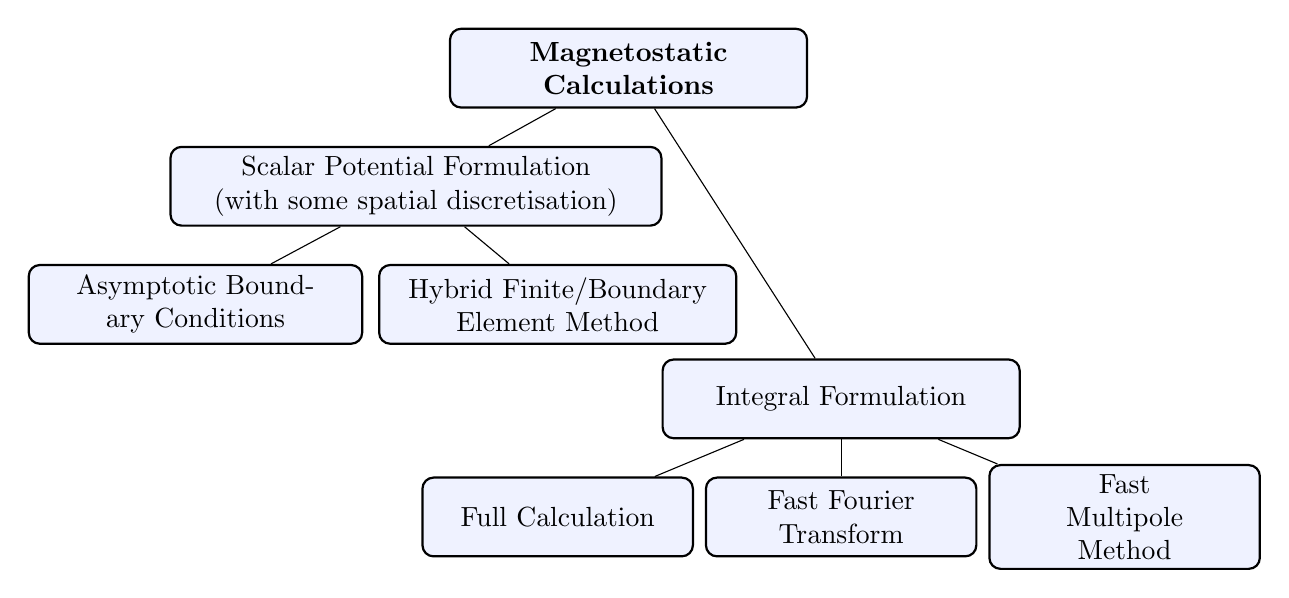
\begin{tikzpicture}[level 1/.style={sibling distance=5.4cm},
    level 2/.style={sibling distance=3.6cm}]

    \node[block] {\textbf{Magnetostatic Calculations}}
    child {node[block,text width=6cm] {Scalar Potential Formulation (with some spatial discretisation)}
      child{node[block,text width=4cm,xshift=-1cm] {Asymptotic Boundary Conditions}}
      child{node[block,text width=4.3cm] {Hybrid Finite/Boundary Element Method}}
    }
    child {node[block,yshift=-2.7cm] {Integral Formulation}
      child{node[block,text width=3.2cm] {Full Calculation}}
      child{node[block,text width=3.2cm] {Fast Fourier Transform}}
      child{node[block,text width=3.2cm] {Fast\\ Multipole\\ Method}}
    };
  \end{tikzpicture}
  \caption{Methods of magnetostatic field calculation that have been used in micromagnetic models.}
  \label{fig:types-mag-stat}
\end{figure}

Integral methods are based on the expression
\begin{equation}
  \Hms(\xv) = \frac{1}{4 \pi} \bigs{ 
    - \int_\magd \nabla' \cdot \Mv(\xv') \frac{(\xv - \xv')}{\abs{\xv -\xv'}^3} \d^3 \xv'
    + \int_\boundd \Mv(\xv') \cdot \nv(\xv') \frac{(\xv - \xv')}{\abs{\xv - \xv'}^3} \d^2 \xv' }.
  \label{eq:Hmsint2}
\end{equation}

After the application of a discretisation scheme the integrals in \cref{eq:Hmsint2} become a sum over all nodes.
The naive way to calculate the magnetostatic fields would then be to work through the list of nodes calculating the field at each of them, so for each node a sum of the contributions from all other nodes must be calculated.
Hence this results in a computation time that scales as $\order{N^2}$ (where $N$ is the number of points used in the space discretisation), this is usually unacceptably slow.

In this section we refer to magnetic charges to mean the macrospins/cells/nodes as appropriate for the spatial discretisation, and $N$ the number of such charges.


\subsubsection{Fast fourier transform methods}

The fast Fourier transform method (FFT) is a simple and efficient method for calculating the magnetostatic field when the magnetic charges are on a regular lattice and the boundary conditions are periodic.

The calculation of $\Hms$ in equation~\cref{eq:Hmsint} can be thought of as applying a convolution operator (\ie $\Hms = D \big[\Mv\big]$).
The matrix corresponding to this operator is only dependent on the geometry, hence it can be precomputed, Fourier transformed and stored.
Then all that is needed to calculate the magnetostatic field is to apply a Fourier transform to $\Mv$, compute the convolution and transform the result back into the time domain by applying the inverse Fourier transform.
Because of the regularity, applying the convolution in the frequency domain is very fast and hence the complexity of the calculation is limited by the complexity of a fast Fourier transform.
This results in a complexity of $\order{N \log(N)}$.
\cite{Jones1997}

The downside of this method is that points to be calculated must be on a regular lattice, similar to the finite difference method.
Hence, it is most suited for use in combination with models using a finite difference spatial discretisation.
Alternatively it may be used in less regular macrospin models by approximating the the macrospins as being on a regular lattice \cite{Jones1997}.


\subsubsection{Fast multipole method}
\label{sec:fast-mult-meth}

An alternative method of calculation of the magnetostatic field is the fast multipole method (FMM).
The fast multipole method takes advantage of the fact that distant magnetic charge has a much smaller effect on the total field at a point than a nearby magnetic charge.

For the field calculation at a specific point the full calculation is only performed for nearby magnetic charges.
Groups of more distant charges are approximated (lumped) as a single multipole placed at the centre of the group.
As the charges become more distant they contribute much less to the field due to the $\frac{1}{(\xv - \xv')^2}$ scaling in equation~\cref{eq:Hmsint2}.
Hence for distant points the a cheaper but less accurate approximation can be used without reducing the accuracy of the final result.

The trick for quickly calculating fields at a large number of points is to pre-calculate multipole approximations for a range of accuracies over all space.
Then the calculation of a field at a single point only requires the full calculation of effects from a few nearby points and from the appropriate multipoles \cite{Beatson1997}.

One advantage of this method over the fast Fourier transform is that it allows for arbitrary geometries.
Also the complexity of the method is $\order{N}$ \cite{Chang2011}, so FMM is more efficent than FFT for sufficiently large problems (although ``sufficiently large'' may in fact be very large due to the cost of computing the required multipole approximations).


\subsection{Scalar potential methods}
\label{sec:magstat-field-calc-pote}

Potential methods are based on the formulation:
\begin{equation}
\begin{aligned}
  \label{eq:Hms2}
  \hms &= - \nabla \phim, \\
  \lap \phim &= \nabla \cdot \mv,
\end{aligned}
\end{equation}
with boundary conditions
\begin{equation}
  \begin{aligned}
    \label{eq:cont-phi-bound2}
    \phim^\inte - \phim^\exte &= 0 \quad \xv \in \boundd, \\
    \pd{\phim^\inte}{\nv} - \pd{\phim^\exte}{\nv} &= \mv \cdot \nv \quad \xv \in \boundd, \\
  \end{aligned}
\end{equation}
and
\begin{equation}
  \begin{aligned}
    \label{eq:phi-inf-bound}
    \phim \rightarrow 0 \text{ as } &\abs{\xv} \rightarrow \infty.
  \end{aligned}
\end{equation}

This is a differential equation and so inside the domain it can be solved simply by applying the finite element or finite difference discretisation methods.
However \cref{eq:phi-inf-bound}, the boundary condition on $\phim$ at infinity, is problematic.
We obviously can not apply this condition directly using standard methods, since that would involve either an infinite number of elements or infinitely large elements.
Hence other techniques must be used, such techniques are the subject of the rest of this section.

The speed of the internal field calculation is $\order{N}$ since it is just a standard FEM or FD calculation, however applying the boundary conditions can require additional processing time.


\subsubsection{Asymptotic boundary conditions}
\label{sec:asymptot-bcs}

One way to avoid an infinite domain is to truncate the external region at some finite distance from the magnetic domain.
However the relationship between truncation distance and accuracy is problem dependent (since the size of the external field at any point depends on the problem geometry) and does not lead to good accuracy even for large truncation distances.

A more sophisticated method is to use asymptotic boundary conditions \cite{Yang1997}. The idea here is to use a truncated external region to calculate the boundary conditions on the magnetic domain that correspond to \cref{eq:phi-inf-bound} being applied at infinity.
Additionally the fact that any solution to the Poisson equation~\cref{eq:Hms2} can be represented as an infinite series of harmonic functions is used to improve the accuracy.
Unfortunately the accuracy of this approach is still quite low, even for large truncation distances \cite{Bottauscio2008}.


\subsubsection{The hybrid finite element method/boundary element method}
\label{sec:bound-elem-meth}

The idea of the hybrid finite element method/boundary element method (FEM/BEM) is to replace the external domain by a dipole layer placed on the surface of the magnetic domain which mimics the effect of the infinite external domain \cite{Fredkin1990}.
This removes the need to truncate or discretise the infinite external domain.
The name comes from the similarity of the use of a dipole layer with the boundary element method, and the fact that the standard finite element method is used to calculate the required potentials in the bulk.
The full details of the method applied to magnetostatic calculations is discussed in \cref{sec:hybr-finit-elem}.

A comparison by Bottauscio\cite{Bottauscio2008} found that using the FEM/BEM method was more accurate than applying asymptotic boundary conditions for a calculation of the time evolution of the magnetisation of a sphere with zero exchange coupling.
Even with a truncation distance of four times the size of the magnetic sphere (the total domain was $4^d$ times larger then the sphere) the accuracy when using asymptotic boundary conditions was worse and did not improve between truncation distances of three and four times the magnetic sphere radius.
Even when exchange coupling was added (giving an easier test) the truncation method was worse than the FEM/BEM method.

The main downside of the FEM/BEM method is that it involves dense matrix of size $N_b \times N_b$ where where $N_b$ is the number of boundary nodes.
This matrix must be stored in memory, and multiplied by a vector for the calculation of the boundary conditions.
The speed of calculation of the boundary values in the method is limited by the dense matrix multiplication which is $\order{N_b^2}$.
Similarly the addtional memory usage is $\order{N_b^2}$, which can limit the size of problems.
Hence the speed of the FEM/BEM method depends on the geometry.

The use of hierarchical matrix techniques can reduce this to $\order{N_b \log(N_b)}$ \cite{Knittel2009}.
In 3D structures which are roughly spherical $N_b = \order{N^{2/3}}$ and so the use of a hierarchical matrix gives optimal computation speed\footnote{With hierarchical matrix techniques the speed is $\order{N^{2/3}\log(N^{2/3})}$ but $\log(x) << x^{1/2}$ for large $x$, hence $\order{N^{2/3}\log(N^{2/3})} << \order{N}$, \ie optimal computation speed scaling.} but for extremely flat structures the number of boundary nodes can be as bad as $N_b = \order{N}$.

Another downside of FEM/BEM is the increase in the complexity of the model: some components of the FEM/BEM method are fundamentally different to FEM, and much additional code and mathematical knowledge may be needed for its implementation.
As an example: singular integrals occur in the boundary element method so more advanced integration methods are needed than for FEM alone.



\section{Compatability of methods}
\label{sec:comp-meth}

While in theory any of the methods discussed above can be combined with any other, there are certain combinations which are problematic.
In this Section we discuss which combinations of methods are especially good or bad.

The use of integral methods with implicit time integration is problematic: the integral formulation couples magnetisation at every point to every other point, meaning that the Jacobian representing the derivatives of each magnetisation with respect to each other magnetisation is completely dense (and hence solution times are extremely slow)!
Explicit time integration methods avoid this issue because no system solve is required.
The most well known example of such a model is OOMMF.


For problems with very simple geometry (\ie thin films, cubeoid shapes) the finite difference method with FFT for magnetostatic calculations is sufficient.
Additionally: for simple geometry there is often no need for well refined meshes, so the problem can be only mildly stiff and explicit time integration methods can be efficient.
This combination of methods is very simple to implement and so is widely used, especially with GPU based code.

For problems with more complex geometry the finite element method must be used for spatial discretisation to obtain good accuracy. 
Magnetostatic calculations on the resulting non-uniform mesh are typically then carried out using either FMM (fastmag) or FEM/BEM (nmag, magpar, femme, \ldots).
The use of refined meshes to fully resolve the geometry can often result in stiff problems, requiring the use of implicit time integration schemes for good efficiency.
In all ``real world'' models using implicit time integration known to the author the Newton-Raphson method is used for linearisation.
Typically some form of preconditioned Krylov solver is then used to solve the resulting linear systems.

??ds rewrite
Many FEM/BEM micromagnetic models use a combination of implicit and explicit schemes: everything except for the magnetostatic field is discretised using an implicit scheme, the magnetostatic field is updated (using an explicit calculation) after each time step. 
This method has the benefit of a larger time-step from the implicit method but the system of equations to be solved is smaller.
However when using this method the adaptive time step calculation must be done specially (\ie not using normal adaptivity) since the system of equations contains no information on the magnetostatic field \cite{Schrefl1997}.
Also stability is no longer guaranteeded because an ad-hoc modification to the time integration method.
Finally any geometric integration properties may be lost (\eg IMR loses the energy property when used in combination with \emph{any} explicit field calculations). 

\subsection{Non-linear solvers and geometric integration}

It should be noted that the geometric properties of IMR derived in \cref{sec:proof-magn-length-ode-imr-llg} and \cref{sec:proof-energy-prop} are only true up to the accuracy with which we solve the LLG.
This is the tolerance of the linearisation method used. 

Additionally the derivations assume that all fields are calculated at the midpoint without any additional approximations, \ie that we are using a fully implicit method.
In contrast to this, many existing models use an explicit approximation to the magnetostatic field in order to avoid including a dense contribution for the long-range magnetostatic interactions\footnote{A dense contribution arises from all accurate magnetostatic calculation methods known to the author, in particular: FEM/BEM, FFT and FMM. See \cref{sec:magn-field-calc} for more details.} in the non-linear solve.
Unfortunately in this case the energy properties will be lost due to the replacement of $\hop \left[ \mpm \right]$ by different approximation (in a similar way to the semi-explicit modification of IMR).
However the magnetisation length property will be retained because it only relies on $\mv$ itself being calculated implicitly.

One way to allow a completely implicit treatment of the magnetostatic field without a dense contribution was explored by d'Aquino \cite{DAquino2005}.
He used a quasi-Newton method where the dense contribution was simply left out of the Jacobian matrix.
This greatly slows down the convergence of the non-linear solve: in the example given in the paper 10-14 iterations were needed (compared to $\sim2$ with a full Newton method).
Additionally in the general case it is not clear that this modified Newton method will converge at all!

In \cref{sec:fully-implicit-bem} we describe and demonstrate a novel efficent and robust solver allowing fully implicit magnetostatic calculations.


% \section{Conclusions}
% \label{sec:model-conclusions}

% A dynamic modelling method will be used because the ability to model time dependent processes is essential.

% For the spatial discretisation a macrospin model is not considered because its application is limited to cases with well separated grains and because it is not able to model effects inside a grain.
% Therefore a finite element spatial discretisation will be used because the ability to treat arbitrary geometries is extremely desirable (for example in the modelling of bit patterned media).
% Additionally \texttt{oomph-lib}\cite{oomph-lib-website} (a multi-physics open source finite element modelling library) gives an excellent framework in which to construct a new finite element micromagnetic model.
% This choice will also allow easy extension to the modelling of heat assisted magnetic recording using a finite element discretisation of the heat equation to model heat flow.

% The magnetostatic field will be evaluated from a scalar potential by the hybrid finite/boundary element method.
% A finite element method will be used because it can be easily integrated into the overall model.
% The hybrid method will be used to apply boundary conditions because the accuracy loss involved in efficiently approximating the external region by asymptotic boundary conditions is large and problem dependent.

% The time discretisation scheme used will be the mid-point method because of it's preservation of magnetisation vector length and ability to deal with stiffness.
% The use of preconditioners to speed up to the solution of the non-linear system created at each time-step will be investigated.


%%% Local Variables:
%%% mode: latex
%%% TeX-master: "main"
%%% End:

\chapter{A finite element method for the Landau-Lifshitz-Gilbert Equation}
\label{sec:galerk-meth-llg}

In this chapter we introduce first give a general introduction to the finite element method.
We then apply the finite element method (with the Newton-Raphson method for linearisation) to the Landau-Lifshitz-Gilbert equation with exchange and a simple magnetostatic field approximation.

\section{Introduction to the finite element method}
\label{sec:intr-finite-ele-diff}

As discussed in \cref{sec:sd-finite-elem-meth} the finite element method (FEM) is a discretisation method which converts a differential equation into a system of algebraic equations.
It allows for more complex geometries than the finite difference method, at the cost of increased complexity.

A simple problem is used to illustrate these methods: solving the Poisson
equation with Dirichlet boundary conditions in one dimension.
This is relevant to 
Find\footnote{A function $g\in C^{k}(0,1)$ if $g$ and it's first $k$ derivatives are continuous on $(0,1)$.} $y(x)\in C^{2}(0,1)$ such that
\begin{equation}
  -y''=f\qquad\text{on }(0,1)
  \label{eq:poisson1}
\end{equation}
\begin{equation*}
  y(0)=y_{a},\quad y(1)=y_{b},\quad f=f(x)\in C(0,1).
\end{equation*}


\subsection{Definitions}
\label{sec:fem-definitions}

The function space $L^{2}$ is the set of all functions $f(x)$ such that $\int_{-\infty}^{\infty}\abs{f(x)}^{2} \d x$ is finite.
The span of a set of functions is the set of all possible linear combinations of the functions. 
If a set of functions $\set{\phi_i}$ is such that $V=\text{span}(\phi_i)$ then we say that $\set{\phi_i}$ spans $V$ and $\set{\phi_i}$ is a basis for the function space $V$.
If $V$ has a basis consisting of a finite number of functions then we say that $V$ is finite dimensional, otherwise $V$ is infinite dimensional.
In a FEM we are interested in approximating an infinite dimensional space (the space of solutions) by a finite dimensional space (the space of approximations).

The $n$-th Sobolev space is the space of all functions such that they and their $n$-th derivatives (in all dimensions) are in $L^2$. For example
\begin{equation}
  \label{eq:H1}
  \sob^1(\magd) = \set{ y \st y, \pd{y}{x_i} \in L^2(\magd) \; \forall x_i }
\end{equation}

\subsection{A weak formulation}
\label{Derivation-of-weighted-residuals}

The method of weighted residuals is a way to convert a differential equation
into an integral form that can be modelled computationally. As such it is the
first step in a variety of modelling methods including the finite element method
and the spectral method.

For simplicity we start, as before, with the one-dimensional Poisson equation
\cref{eq:poisson1}, with homogeneous Dirichlet boundary conditions
(\ie $y_{a}=y_{b}=0$).

The formulation used in \cref{eq:poisson1} (called a strong formulation) is too restrictive for our purposes.
It disallows some useful approximating functions, and in higher dimensional cases restricts the geometries that can be modelled \cite{HowardElmanDavidSilvester2006}. 
For ``well behaved'' functions the following weak formulation is equivalent but without these restrictions: find $y\in V_{s}$ such that
\begin{equation}
  -\int_{0}^{1}y''v\, dx=\int_{0}^{1}fv\, dx \qquad \forall v\in V_{T}.
  \label{eq:26}
\end{equation}

Here $V_{T}$ is some appropriate space of \emph{test functions}.
The test functions must satisfy $V_{T}\subseteq \sob^0(0,1)$, in order to ensure that the integrals in \cref{eq:26} are well defined. 
Additionally \cref{eq:26} should not depend directly on the boundary values since they are fixed, this can be done by forcing the test functions to be zero on the boundaries.
So an appropriate test function space is
\begin{equation}
  \label{eq:28}
  V_{T}=\set{v : [0,1] \rightarrow \real \st v \in \sob^0(0,1),\; v(0) =0,\; v(1)=0}.
\end{equation}

The space $V_{s}$ is the solution space
\begin{equation}
  V_{s}=\set{ y : [0,1] \rightarrow \mathbb{R} \st y \in \sob^2(0,1),\, y(0) = y_{a},\, y(1) = y_{b}},
\end{equation}
\ie the space of functions that are sufficiently smooth for the integrals to be finite and that satisfy the boundary conditions.

To see that the weak form is equivalent to \cref{eq:poisson1} consider the case when $f(x) + y''(x)$ is non-zero at a point $x \in (0,1)$, \ie when the strong form \cref{eq:poisson1} is not satisfied. 
Since \cref{eq:26} must hold for all functions we can choose a function which is non-zero at $x$ and hence the equality in \cref{eq:26} will fail.
So $f(x) + y''(x) = 0$ must hold at all points $x \in (0,1)$.
We call this the method of weighted residuals because we use an integral of the residual weighted by a test function to approximate the true equation \cite[210, 214]{Zeinkiewicz1967}.

The smoothness restrictions on our weak form approximation can be further reduced using the integration by parts formula:
\begin{equation}
  \intui{qp'} = \Big[ pq \Big]_{0}^{1} - \intui{p q'},
\end{equation}
applied to the left hand side of \cref{eq:26}.
Let $p=y'$ and $q=v$, then
\begin{equation}
  -\intui{ y''v } = -\Big[ y'v \Big]_{0}^{1} + \intui{ y'v' }.
  \label{eq:29}
\end{equation}

Using the fact that the test functions must be zero at the boundaries the square bracketed term in \cref{eq:29} is zero and we are left with
\begin{equation}
  -\intui{ y''v } = \intui{ y'v' }.
\end{equation}
 
Hence our problem can be reduced to the following: find 
\begin{equation}
y\in V_{S}'=\set{y \st y \in \sob^1(0,1),\, y(0) = y_a, y(1) = y_b },
\end{equation}
such that
\begin{equation}
  \intui{ y'v' } = \intui{ fv } \qquad 
  \forall v \in V'_{T} = \set{v \st v \in \sob^1(0,1),\, v_a=v_b=0}.
  \label{eq:symmetric-weak-poisson}
\end{equation}

Note that this rearrangement has removed the second derivative in $y$, hence we only require $y \in \sob^1(0,1)$ instead of $y \in \sob^2(0,1)$.
This allows a wider range of shape functions to be used but comes at the expense of requiring more smoothness in the test functions.
Also note that if $y_a = y_b = 0$ then $V_{S}'=V_{T}'$, our test and solution spaces are identical.

An alternative class of boundary condition, called Neumann conditions, specify the values of $y'$ at the boundary.
This allows the bracketed term in \cref{eq:29} to be calculated directly.
In this case we do not force the test functions to be zero on the boundary.

\subsection{A Discretisation}

\Cref{eq:symmetric-weak-poisson} is still inapplicable as a computational method since the test and solution spaces are infinite dimensional (\ie the problem is still continuous).
So for the next step we approximate $V_{T}'$ by a finite dimensional function space $V_{T}^{h}\subset V_{T}'$ such that
\begin{equation}
  V_{T}^{h}=\text{span} \set{ \tbf_{\ndi} }_{n=0}^{N}
  = \set{v_h \st v_h = \sum_{n=0}^{N}\alpha_{\ndi} \tbf_{\ndi},\, \alpha_{\ndi} \in \real,\,
    v_a = v_b =0 },
  \label{eq:30}
\end{equation}
for some finite set of test basis functions $\tbf_{\ndi}$.
The distinction between the test functions and the test basis functions is often dropped.
Similarly, for $V_S$
\begin{equation}
  \label{eq:34}
  V_{S}^{h}=\text{span} \set{ \sbf_{l} }_{l=0}^{N_l}
  = \set{y_h \st y_h = \sum_{l=0}^{N_l}y_{l} \sbf_{l},\, y_{l} \in \real,\,
    y(0) = y_a,\, y(1) = y_b }.
\end{equation}
We call $\sbf_l$ the shape functions.
Different choices of $\tbf_{\ndi}$ and $\sbf_l$ lead to different methods, the choice corresponding to the finite element method will be discussed in \cref{sub:Actual-Finite-Elements}.
For now we continue with the conversion of the problem into a general discrete form.

Replacing $v_{h}$ from \cref{eq:poisson1} by $\tbf_{\ndi}$ gives an equivalent set of conditions
\begin{equation}
  \intui{  y'_{h} \tbf_{\ndi}'  }  = \intui{ f\tbf_{\ndi} } \qquad n=0,\ldots,N,
  \label{eq:discrete_weak_test_fns_replaced}
\end{equation}
Since $y_{h}\in V_{S}^{h}$ we can also replace $y_{h}$ by a linear combination of the shape functions, \ie
\begin{equation}
  y_{h}=\sum_{l=0}^{N_l} y_{l}\sbf_{l},
  \label{eq:y-spans}
\end{equation}
where $c_l \in \real$ are (unknown) coefficients.
Substituting \cref{eq:y-spans} into \cref{eq:discrete_weak_test_fns_replaced} gives
\begin{equation}
  \sum_{l=0}^{N_l} y_{l}\intui{ \sbf_{l}'\tbf'_{\ndi} } =\intui{ f\tbf_{\ndi} } 
  \qquad n=0,\ldots,N.
  \label{eq:31}
\end{equation}

The functions $f$, $\tbf$ and $\sbf$ are known and so the integrals in \cref{eq:31} are just numbers (which must be calculated at some point, see \cref{sec:numer-eval-integrals}).
Hence we introduce a matrix $\Am$ and a vector $\mathbf{b}$ containing these numbers:
\begin{equation}
  \begin{aligned}
    \Am_{l\ndi} &= \intui{ \sbf_{l}'\tbf'_{\ndi} }, \\
    b_{j} &= \intui{ f\tbf_{\ndi} }. \\
    \label{eq:Aij_bj}
  \end{aligned}
\end{equation}
and the problem is reduced to a system of linear equations
\begin{equation}
  \Am \yv = \bv.
  \label{eq:final_galerkin}
\end{equation}
This can be solved to find the vector of unknown coefficients $\yv$ which can be substituted into \cref{eq:y-spans} to give an approximation for $y(x)$.


\subsection{Finite Elements in One Dimension}
\label{sub:Actual-Finite-Elements}

To create a usable implementation of the methodology derived in \cref{Derivation-of-weighted-residuals} we must first define basis functions for the spaces $V_{T}^{h}$ and $V_S^h$.
We choose the test and solution basis functions to be the same: $\sbf_l = \tbf_l$.
This choice defines a Galerkin method (and results in a symmetric matrix $\Am$ if the original equation has the corresponding symmetry) \cite[215]{Zeinkiewicz1967}.

The overall aim is to approximate an arbitrary function by a linear combination of a finite set of easy-to-work-with functions, $\tbf_\ndi$.
A good class of functions to satisfy this requirement is the polynomials: they are trivial to add, subtract and differentiate; and can be easily numerically integrated (see \cref{sec:numer-eval-integrals}).

Additionally it is desirable that the final matrix $\Am$ be sparse (to allow efficient linear algebra).
For this to happen we need $\intui{ \sbf_{l}'\tbf'_{\ndi} } = 0$ for most pairs of $l, \ndi$. 
An obvious way to achieve this is to have each basis function only overlap (in space) with a few other basis functions, for example by having each basis function non-zero only on a small region.
Basis functions with this property are said to have ``local support''.

These two points lead us to the use of a carefully constructed set of \emph{piecewise polynomials} as our basis functions.
We first split the domain into $N_e$ regions called \emph{elements}, each with a \emph{node} at either end.
We then define two ``local'' basis functions within each element as
\begin{equation}
  \tbf^{(e)}_{0}=\dfrac{x-x^{(e)}_{1}}{x^{(e)}_{0}-x^{(e)}_{1}},\qquad
  \tbf^{(e)}_{1}=\dfrac{x-x^{(e)}_{0}}{x^{(e)}_{1}-x^{(e)}_{0}},
  \label{eq:simple_lagrange}
\end{equation}
where $x^{(e)}_0$ and $x^{(e)}_1$ are the positions of the nodes of element $e$.
This definition results in a useful property of $\tbf^{(e)}_{\ndi}(x)$:
\begin{equation}
  \label{eq:35}
  \tbf^{(e)}_{\ndi}(x_{\ndi}) =
  \begin{cases}
    1 & k = \ndi, \\
    0 & k \neq \ndi,
  \end{cases}
\end{equation}
since at $x_{\ndi}$ with $k \neq \ndi$ the numerator is zero and at $x = x_{\ndi}$ the numerator and denominator are equal.
Next we define the $\ndi$th (global) basis function as:
\begin{equation}
  \label{eq:33}
  \tbf_\ndi(x) =
  \begin{cases}
    \tbf_\ndi^{(e)}(x) & \text{if $x \in [x^{(e)}_0, x^{(e)}_1]$ and node $\ndi$ is in element $e$,} \\
    0 & \text{otherwise.}
  \end{cases}
\end{equation}
So each basis function is only non-zero on the elements neighbouring the node where it has a maximum value.
We call the set of such polynomial basis functions $\tsbasis$.

\begin{figure}
  \center
  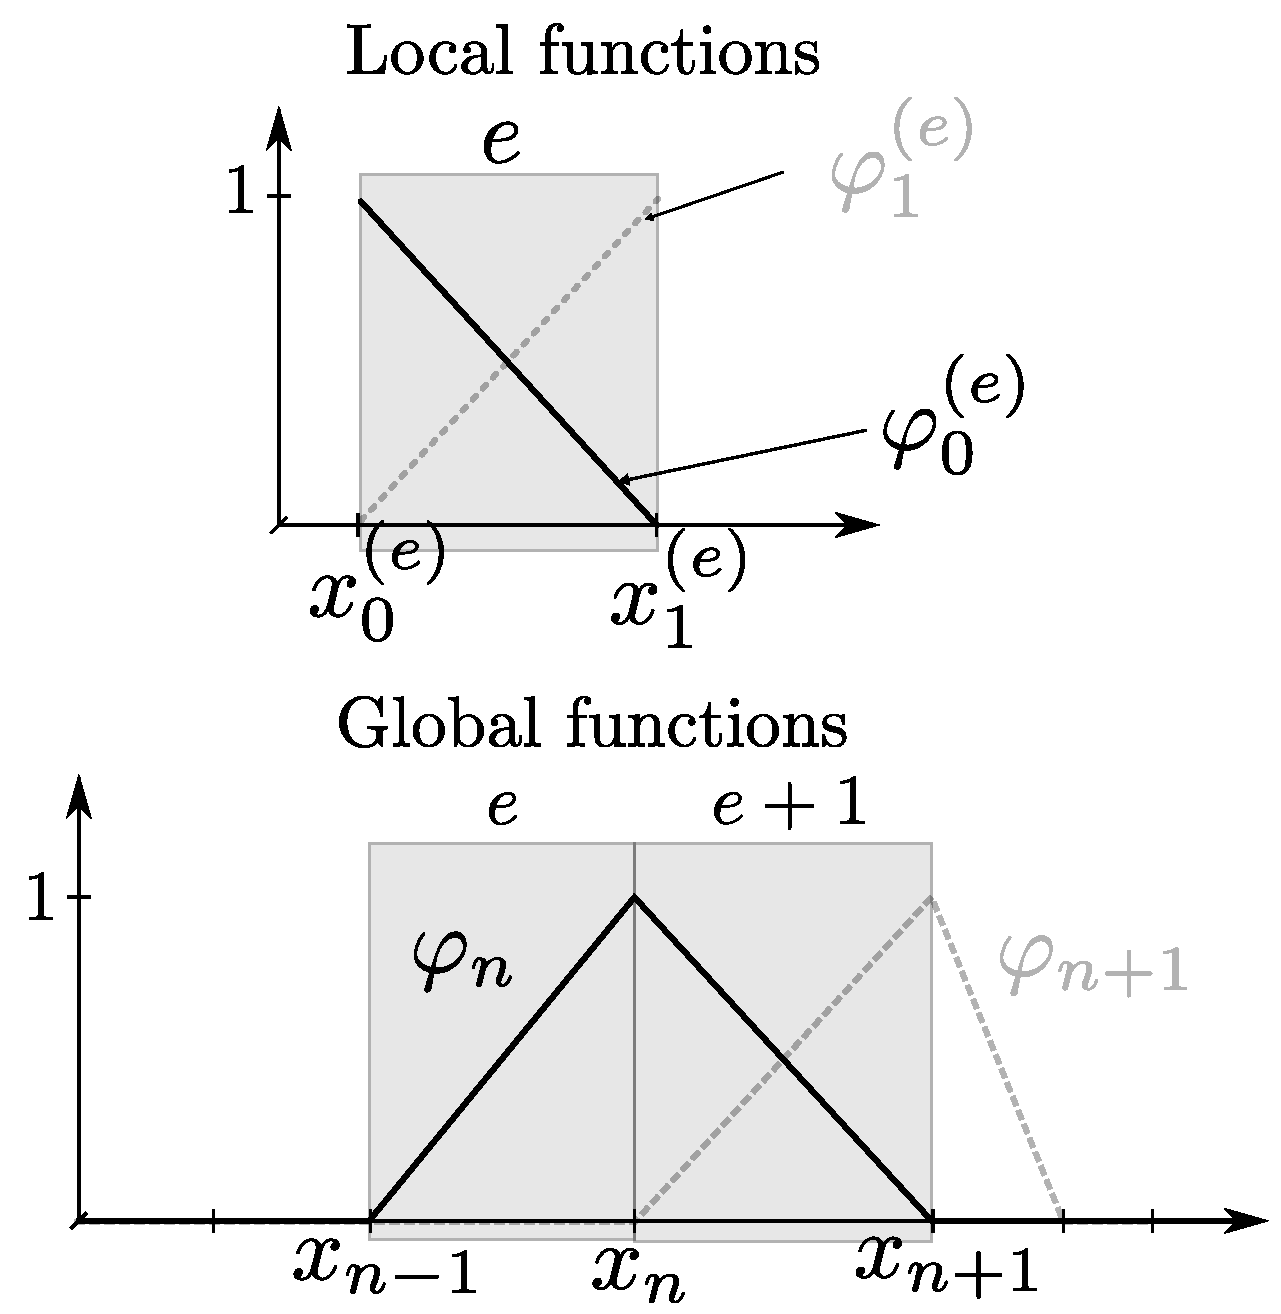
\includegraphics[width=0.8\textwidth]{./images/local_global_functions}
  \caption{The local and global piecewise polynomial basis functions and numbering schemes for a one-dimensional finite element model.   % ??ds numbering: change e_i to element e, e_{i+1} to e+1, x_i to x_\ndi, x^(i) to x^(e) L_i to \tbf_\ndi
  }
  \label{fig:local_global_functions}
\end{figure}



% \begin{figure}
%   \center
%   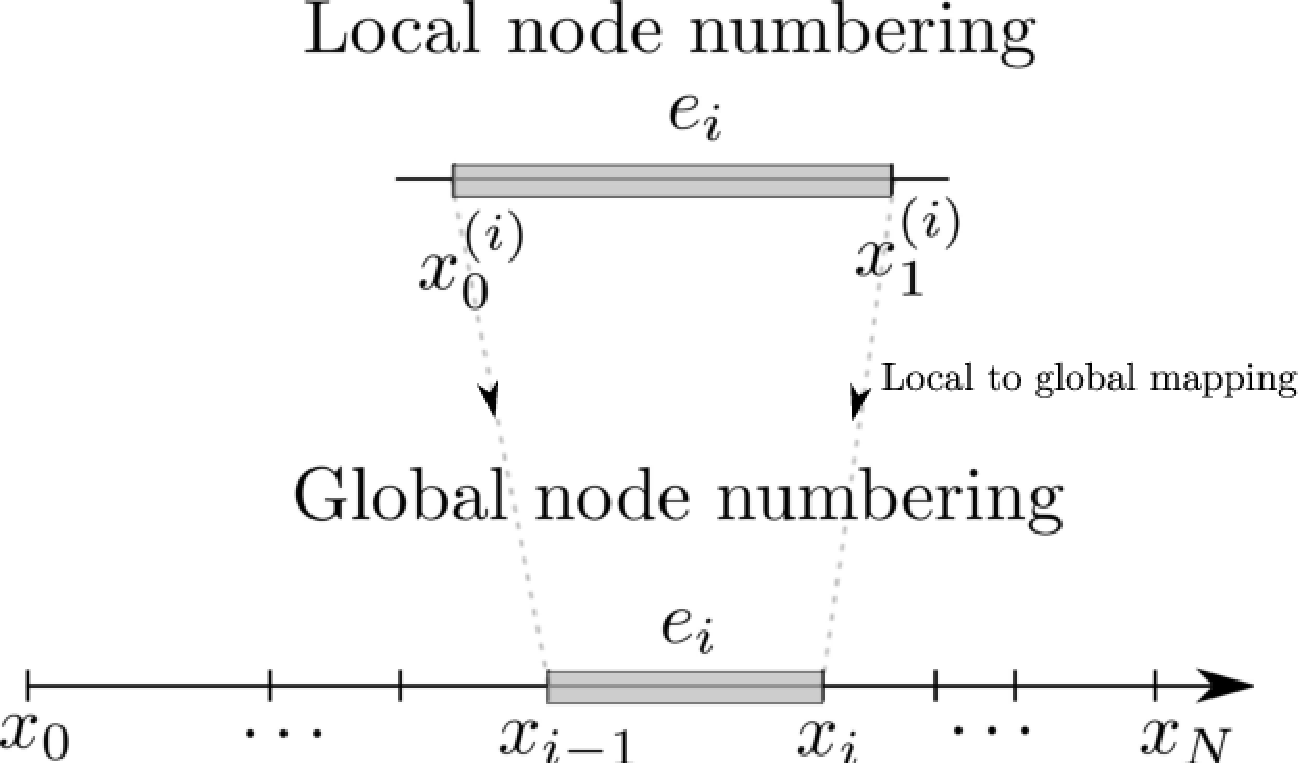
\includegraphics[width=0.8\textwidth]{./images/local_global_numbering}
%   \caption{The local and global numbering schemes for nodes in a one-dimensional
%     finite element model.}
%   \label{fig:local-global-numbering}
% \end{figure}

The basis functions for are clearly integrable (\ie in $L^2[0,1]$) since they are just a combination of local basis functions, which are obviously integrable.
So to obtain sets of functions which are subsets of $V_T^h$ and $V_S^h$ we merely need to remove the test functions which are non-zero on Dirichlet boundaries.

It is advantageous to work with such low order polynomials even for very complex models because evaluation of integrals and interpolated values is simple and cheap to compute.
Also note that an arbitrary level of accuracy can be achieved when approximating the a smooth function by piecewise polynomials by increasing the number of polynomials used (\ie after sufficient mesh refinement).

The description here generalises to higher dimensions fairly easily: nodes are placed at every corner/vertex of the element and the polynomials used are replaced by higher dimensional ones with equivalent properties \cite[20]{HowardElmanDavidSilvester2006}.

To calculate the matrix $\Am$ and the vector $\mathbf{b}$ from equation \cref{eq:Aij_bj} needed for \cref{eq:final_galerkin} we first calculate the local contributions from each element: $\Am^{(e)}$ and $\mathbf{b}^{(e)}$.
Then we only require a local-to-global mapping tells us which local nodes map to a given global node and the global matrix $\Am$ and vector $\mathbf{b}$ can be assembled by summing the appropriate local contributions.

For our one-dimensional Poisson case the calculation of $\Am^{(e)}$ is quite
simple, substituting the two local basis functions \cref{eq:simple_lagrange} into
\cref{eq:Aij_bj} and using $h=x_{1}^{(e)}-x_{0}^{(e)}$ we are left with
\begin{equation}
  \Am^{(e)} = \dfrac{1}{h}
  \left[
    \begin{array}{cc}
      1 & -1 \\ -1 & 1
    \end{array}
  \right],
\end{equation}
where $h$ is the element size, $h = x_{1}^{(e)}-x_{0}^{(e)}$ (note that $h$ can vary between elements).
Similarly for $\mathbf{b}^{{e}}$ we obtain
\begin{equation}
  \mathbf{b}^{(e)}=\dfrac{1}{h}\left[
    \begin{array}{c}
      -\int_{x_{0}^{(e)}}^{x_{1}^{(e)}}(x-x_{1}^{(e)})\, f(x)\, dx\\
      \int_{x_{0}^{(e)}}^{x_{1}^{(e)}}(x-x_{0}^{(e)})\, f(x)\, dx
    \end{array}\right],
\end{equation}
which we must compute numerically since the entries depend on $f(x)$ which is not fixed.



\subsection{Numerical evaluation of integrals}
\label{sec:numer-eval-integrals}

In the above example the integrals for $\Am$ were fixed and so could be calculated analytically.
This is not the case in general (\eg the vector $\bv$, or the matrix for non-linear problems), so we need some method to computational evaluate the integrals.
The most flexible way to evaluate integrals is to do it purely numerically using a quadrature scheme.
A quadrature scheme is an approximation to an integral of the form
\begin{equation}
  \begin{aligned}
    \intdx{f(\xv)} &\approx  \sum_i w_i f(\xv_i),
  \end{aligned}
\end{equation}
where the selection of the ``knots'' $\xv_i$ and the weights $w_i$ depend on the scheme.

There exist many different quadrature schemes suited for different applications.
However because we only ever need to evaluate integrals of polynomial functions a single simple and extremely accurate class of quadrature is sufficient: Gaussian quadrature \cite[492]{Kincaid2002}.
Gaussian quadrature is the quadrature scheme derived by choosing the knots such that when $n$ knots are used it is able to exactly evaluate integrals of polynomials up to order $2n + 1$ (this is the highest possible order).

In higher dimensions the integration is not quite so simple.
Quadrature schemes only apply over specifically shaped domains (or at least must be non-trivially modified for alternative geometries).
To get around this issue we use a coordinate transformation to a reference element \cite[29]{HowardElmanDavidSilvester2006}.
So \eg any four sided element is mapped to the square $[-1, 1] \times [-1, 1]$, and standard quadrature schemes can be used.
The final difficulty is to calculate the Jacobian of the transformation: if the ``local'' position variable is $\sv$ then the Jacobian is
\begin{equation}
  J = \abs{ \pd{\sv}{\xv}} = \frac{1}{\abs{\pd{\xv}{\sv}}},
\end{equation}
where the elements of the Jacobian matrix $\pd{\xv}{\sv}$ can be calculated by interpolating $x$ using the local shape functions and differentiating.

So the final integration scheme is
\begin{equation}
  \begin{aligned}
    \intdx[\magd_e]{f(\xv)} &= \intds[\magd_e]{f_s(\sv) J_e(\sv)}, \\
    &\approx  \sum_{i=0}^N w_i f_s(\sv_i) J_e(\sv_i).
  \end{aligned}
\end{equation}
where the definition of $f_s(\sv)$ is
\begin{equation}
  f_s(\sv) = f\bigb{\sum_j  \xv_j \sbf_j(\sv)}.
\end{equation}

Gaussian quadratures for square and cube elements can be trivially constructed from the one dimensional quadrature using a tensor product formula.
Similar ``full integration'' quadratures for triangular and tetrahedral elements exist \eg \cite{oomph-lib-integral.cc}.




\section{Application to spatial discretisation of the LLG}
\label{sec:llg-initial-equations}

We now apply the finite element method as discussed in \cref{sec:intr-finite-ele-diff} (together with the Newton-Raphson discussed in \cref{sec:newt-raph}) to the Landau-Lifshitz-Gilbert equation.
We start with the Gilbert form of the LLG \cref{eq:Gilbert} with the various effective fields and the potential method for calculating the magnetostatic field \cref{eq:Hms}.
We use the Gilbert form of the LLG even though it is less intuitive because only contains single cross product terms, reducing the complexity of derivations.
A side effect of this choice is that explicit time integration schemes cannot be used since the time derivative is only defined implicitly.

\subsection{Initial equations}

After non-dimensionalisation (see \cref{sec:land-lifsh-gilb-normalisation}) the Landau-Lifshitz-Gilbert equation with effective fields is given by
\begin{equation}
  \begin{aligned}
    \dmdt &= - \mv \times \hv + \alpha \mv \times \dmdt, \\
    \hv &= \happ - \nabla \phim + \lap \mv + \kone (\mv \cdot \ev) \ev, \\
    \lap \phim &= \div \mv.
    \label{eqn:ndllg-starting}
  \end{aligned}
\end{equation}

For now we consider the magnetostatic potential only within the magnetic domain, $\magd$, with Neumann or Dirichlet boundary conditions on the boundary, $\boundd$. 
Details of the extension to include the effects of the external region using the FEM/BEM method are given in \cref{sec:hybr-finit-elem}, both Dirichlet and Neumann cases will be required.
We define $\boundd_D$ and $\boundd_\Neu$ respectively to represent the region of the boundary domain where a Dirichlet condition or Neumann is imposed on the potential.
So on $\boundd_\Neu$ $\nabla \phim(\xv) \cdot \nv = g_\Neu(\xv)$ and on $\boundd_D$ $\phim(\xv) = g_D(\xv)$.
We also define the following function spaces for convenience
\begin{equation}
\begin{aligned}
  \label{eq:037}
  \Dfs & = \set{ v \st v(\xv) = g_D(\xv) \; \forall \xv \in \boundd_D }, \\
  \Dfs_0 &= \set{ v \st v(\xv) = 0 \; \forall \xv \in \boundd_D }.
\end{aligned}
\end{equation}
??ds think this is wrong for solution space: can't we just use the full set and say that the Dirichlet boundary node values are fixed? 

Recall from \cref{sec:magn-bound-cond} that the boundary condition on the magnetisation is
\begin{equation}
  \label{eq:m-bc}
  \mv \times \dmdn = \zerov,
\end{equation}
It turns out that this Neumann-like condition is exactly what is needed in the derivation of the residuals.
No special function space is needed for the solutions and test functions of $\mv$ since only Neumann conditions are used.


\subsection{Weak form residuals and relaxed smoothness requirements}

We now convert equations \cref{eqn:ndllg-starting} into their residual weak forms as described in \cref{Derivation-of-weighted-residuals}.
In the following we will need the identity\footnote{This can be easily derived by applying the product rule to $\nabla \cdot (v \nabla \phim)$.}
\begin{equation}
  (\lap \phim) \test = \nabla \cdot (v \nabla \phim) - \nabla \phim \cdot \nabla v.
  \label{eq:20}
\end{equation}
We will also make use of the divergence theorem
\begin{equation}
  \intd{\div \fv} = \intb{\fv \cdot \nv}.
  \label{eq:div-thm}
\end{equation}

The Newton residual for the magnetostatic potential is given by
\begin{gather}
  \rphi(\phim) = \intd{ (\lap \phim) \test }
  - \intd{ (\nabla \cdot \mv) \test}, \label{eqn:phires1}
\end{gather}
where $\phim \in \sob^2(\magd) \cap \Dfs$ and $\mv$ is some sufficiently smooth function.

Recall that problem is to find some $\phim$ such that the residual is zero $\forall \test \in \sob^0(\magd) \cap \Dfs_0$.
We will find such a $\phim$ using the Newton-Raphson method.
Note that while the use of a linearisation method is unnecessary for the magnetostatic potential alone (since \cref{eqn:phires1} is linear in $\phim$) it becomes necessary once the LLG itself is included.

The use of \cref{eqn:phires1} for calculating $\rphi$ would require the existence of second order derivatives.
We prefer to reduce the order of these derivatives as discussed in \cref{Derivation-of-weighted-residuals} to relieve the smoothness requirements on our solution.
As before we do this by ``transferring'' the derivatives onto the test functions \cite{HowardElmanDavidSilvester2006}.

Integrating identity \cref{eq:20} over the domain and applying the divergence theorem \cref{eq:div-thm} we obtain
\begin{equation}
  \begin{aligned}
    \intd{ (\lap \phim) \test} &=  \intd{\nabla \cdot (\test \nabla \phim)}
           - \intd{\nabla \phim \cdot \nabla \test},\\
    &= \intb{\test (\nabla \phim \cdot \nv)} 
    - \intd{ \nabla \phim \cdot \nabla \test}.
    \label{eqn:identitygauss}
  \end{aligned} 
\end{equation}
Next substituting \cref{eqn:identitygauss} into \cref{eqn:phires1} gives
\begin{equation}
  \rphi(\phim) = \intb{ \test (\nabla \phim \cdot \nv) }
  - \intd{ \nabla \test \cdot \nabla \phim }
  - \intd{ (\nabla \cdot \mv) \test }.
\end{equation}
This contains only first order derivatives so the solution space for $\phim$ is relaxed to $\sob^1(\magd) \cap \Dfs$. 
However all first partial derivatives of the test functions are now required to be integrable, \ie $v \in \sob^1(\magd)$ instead of $v \in \sob^0(\magd)$.

Note that the boundary integral is always zero on the Dirichlet region of the boundary by our definition of the test functions. 
Hence the boundary integral is only non-zero over $\boundd_{\Neu}$ where we know $\nabla \phim \cdot \nv = g_{\Neu}$.
So the final residual is
\begin{equation}
  \rphi(\phim) = \int_{\boundd_\Neu} \test g_\Neu \d \boundd
  - \intd{ \nabla \test \cdot \nabla \phim}
  - \intd{ (\nabla \cdot \mv) \test}.
  \label{res:contphi}
\end{equation}


Next we apply the same process to the Landau-Lifshitz-Gilbert equation with effective fields, \cref{eqn:ndllg-starting}.
For now we sidestep the details of time discretisation by assuming $\dmdt$ to be just another function of $\xv$.
The weak form of the LLG is
\begin{equation}
  \rllgv(\mv, \test) = \int_\magd \Big( \dmdt
  + (\mv \times \hca) + (\mv \times \happ) \\
  - (\mv \times \nabla \phi) + (\mv \times \lap \mv)
  - \dampc \left( \mv \times \dmdt \right)
  \Big) \test \d\magd
  . \label{res:contllg}
\end{equation}
Similarly to the previous examples the idea is to apply the Newton-Raphson method to find $\mv \in \sob^2(\magd)$ such that $\rllgv(\mv, \test) \approx 0$ $\forall \test \in \sob^0(\magd)$.

Note that in \cref{res:contllg} the residual is a vector.
However it is equivalent to write
\begin{equation}
  \rllg(\mv, \testv) = \int_\magd \Big( \ldots  \Big) \cdot \testv \d\magd,
\end{equation}
where $\testv \in (\sob^0(\magd))^3$ and the bracketed term is exactly the same as in \cref{res:contllg}.
To see that $\rllg(\mv, \testv) = 0\; \forall \testv \in (\sob^0(\magd))^3$ implies $\rllgv(\mv, \test) = 0 \; \forall \test \in \sob^0(\magd)$ consider three vector test functions: $(\test, 0, 0)$, $(0, \test, 0)$ and $(0, 0, \test)$.
Clearly $\rllg(\mv, (\test, 0, 0)) = \rllg(\mv, \testv)[0]$, and similarly for the other two cases.
To see the inverse relationship (\ie $\rllgv(\mv, \test) = 0 \ldots$ implies $\rllg(\mv, \testv) = 0 \ldots$) note that if $\rllg(\mv, \test) = 0\; \forall \test \in \sob^0(\magd)$ then each term of every dot product in $\rllg(\mv, \testv)$ is zero and so the total residual is zero $\forall \testv \in (\sob^0(\magd))^3$.
The use of vector test functions makes certain manipulations simpler so, for the remainder of this section, we will work with vector test functions.

We again wish to reduce the order of the required derivatives, this time on $\mv$ in the term
\begin{equation}
  I = \intd{ (\mv \times \lap \mv) \cdot \testv }.
  \label{eq:46}
\end{equation}
First we reorder the terms to give
\begin{equation}
  \begin{aligned}
    I &= \intd{\lap \mv \cdot (\testv \times \mv)}, \\
      &= \intd{\lap \mv \cdot \bv}, \\
      &= \sum_{i=0}^2 \intd{ b_i (\lap m_i)},
  \end{aligned}
\end{equation}
where $\bv = (\testv \times \mv)$.
Note that this is very similar to \cref{eqn:phires1}, and so we can apply the same operations as were used to obtain reduced derivatives in the Poisson case. 
Doing so we obtain
\begin{equation}
  I = \sum_{i=0}^2 \intb{b_i (\grad m_i \cdot \nv)} - \intd{\grad b_i \cdot \grad m_i}.
\end{equation}

It turns out that the first term is exactly the weak form of \cref{eq:m-bc}, the boundary condition on $\mv$:
\begin{equation}
  \begin{aligned}
    \sum_{i=0}^2 \intb{b_i (\grad m_i \cdot \nv)} 
    &= \intb{\bv \cdot \pd{\mv}{\nv}}, \\
    &=  \intb{(\testv \times \mv) \cdot \pd{\mv}{\nv}}, \\
    &=  \intb{(\mv \times \pd{\mv}{\nv}) \cdot \testv} = 0 .
  \end{aligned}
\end{equation}

Next we need an expression for $\grad b_i$.
To avoid switching to tensor notation it is helpful to define, for any vector $\av$: $\grad \av = (\grad a_0, \grad a_1, \grad a_2)$.
Then using the product rule we have
\begin{equation}
  \begin{aligned}
    \grad \bv &= \grad \bigb{\testv \times \mv}, \\
    & = (\grad \testv) \times \mv + \testv \times (\grad \mv).
  \end{aligned}
\end{equation}
Hence
\begin{equation}
  I = - \intd{\grad \mv : \bigb{\grad \testv \times \mv}} 
      - \intd{\grad \mv : \bigb{\testv \times \grad \mv}},
      \label{eq:72}
\end{equation}
where ``$:$'' is the component-wise scalar product, \eg $\grad \av : \grad \cv = \grad a_0 \cdot \grad b_0 + \grad a_1 \cdot \grad b_1 + \grad a_2 \cdot \grad b_2$.

Note that the $:$ operator obeys the usual triple product identity
\begin{equation}
  \av : (\av \times \bv) = \zerov,
  \label{triple:-identity}
\end{equation}
and permutations of \cref{triple:-identity}, because
\begin{equation}
  \begin{aligned} 
    \threevecnum{\av} : \bigb{\threevecnum{\av} \times \bv} &= \av_0 \cdot (\av_0 \times \bv) + \ldots, \\
    & = 0 + 0 + 0
  \end{aligned}
\end{equation}
Hence the second term of \cref{eq:72} is zero, so after reordering terms we are left with
\begin{equation}
  \label{eq:final-lap-residual}
  I = - \intd{\bigb{\mv \times \grad \mv} : \grad \testv}.
\end{equation}

So the final residual for the LLG equation, using a vector test function, is
\begin{equation}
  \begin{aligned}
    \label{eq:llg-res-final}
    \rllg(\mv, \testv) &= \int_\magd \dmdt\cdot \testv
    + (\mv \times \hca)\cdot \testv 
    + (\mv \times \happ)\cdot \testv 
    - (\mv \times \nabla \phi)\cdot \testv \\
    & - \bigb{\mv \times \grad \mv} : \grad \testv
    - \dampc \left( \mv \times \dmdt \right)\cdot \testv
    \d\magd.
  \end{aligned}
\end{equation}

The final problem statement is: 
\begin{equation}
  \eqpar{Find $\mv \in (\tsinf)^3$, $\phim \in \tsinf \cap \Dfs$ such that $\rllg(\mv, \testv) = 0$ for all $\testv \in (\tsinf)^3$ and $\rphi(\phim, \test) = 0$ for all $\test \in \tsinf \cap \Dfs_0$.}
\label{eq:inf-dim-problem}
\end{equation}




\subsection{Spatial Discretisation}
\label{sec:spat-discr-resi}

The next step is to choose a finite dimensional approximation, $\ts$, for the infinite dimensional test and solution function spaces, $\tsinf$, such that the residuals \cref{res:contphi,eq:llg-res-final} become discrete in space.
Just as in \cref{sub:Actual-Finite-Elements} we represent the finite dimensional spaces using a set of piecewise linear polynomials, $\tsbasis$, as basis functions.

The approximations to the unknown functions $\mv$ and $\phim$ are represented as a sum over the shape functions $\sk \in \tsbasis$ (or $\tsbasis \cap \Dfs$ for $\phim$ with Dirichlet conditions) as
\begin{equation}
  \begin{aligned}
    \mv &\approx \sum_{k = 0}^{N} \sk \, \mv_k, \\
    \phim &\approx \sum_{k = 0}^{N} \sk \, \phim_{k}.
    \label{eq:unknowns-basis}
  \end{aligned}
\end{equation}
Similarly the approximations to the test functions are represented as a sum over the test basis functions, $\tn \in \tsbasis$ (or $\tsbasis \cap \Dfs_0$ as applicable), as
\begin{equation}
  \label{eq:47}
  \test \approx \sum_{\ndi = 0}^{N} \tn \, a_\ndi.
\end{equation}
Note that in our method $\sbf_k \equiv \tbf_k$ except for Dirichlet boundary $\phim$ shape functions, but we continue to write them differently for generality.
In one dimension the $\sk$ and $\tn$ are as given in \cref{eq:simple_lagrange}.
The extension to higher dimensions is straightforward: see \eg \cite[25]{HowardElmanDavidSilvester2006}.

So substituting the basis representations, \cref{eq:unknowns-basis,eq:47} into the continuous residuals we obtain approximations for the residuals in terms of a finite number of nodal values.\footnote{We do not write this form out here as it is long, messy and does not illuminate anything.}
Next we replace the requirement that the residuals be zero for all test functions in the infinite dimensional set $\tsinf$ with the equivalent requirement for all functions in the finite set $\tsbasis$. 
This results in a finite number of conditions (the residuals) on a finite number of variables (the nodal values) and so the spatial discretisation is complete.

As described in \cref{sub:Actual-Finite-Elements} we also convert this ``global'' representation into a ``local'' representation on each element.

% Let $\magd_\eli$ represent the volume of element $e$, let $\boundd_\eli$ represent any part of the boundary of the element which is on $\boundd$ (nothing for most elements).
% Then the contribution of element $\eli$ to the residuals at node $\ndi$ is exactly as given in equations~\cref{res:tintro}-\cref{res:tllg} except that the integrations are performed over $\magd_\eli$ and $\boundd_\eli$ rather than $\magd$ and $\boundd$.
% Also note that the sums only need to consider values of $k$ such that node $k$ is in element $\eli$ and that residual contributions only need to be calculated for nodes $\ndi$ such that node $\ndi$ is in element $\eli$.


\section{Time Discretisation}
\label{sec:time-discretisation-resi}

In this section we discuss how to deal with the time derivative in the LLG residual \cref{eq:llg-res-final}.
As discussed in \cref{sec:numer-meth-micr}, we will apply standard time integration methods used for ODEs.
This application of independent spatial and time discretisations is known as semi-discretisation or the method of lines.

We cannot simply apply the time integration methods in the way they are written in \cref{sec:some-implicit-time-integrators} (and in most text books) because our LLG residual \cref{eq:llg-res-final} cannot be written in the required form $\pd{\yv}{t} = \fv(t, \yv)$ since it is an implicit function of the time derivative.\footnote{Actually we could have started with the LL form \cref{eq:LLG} where the derivative can be given explicitly, but as mentioned above this method is simpler.}
Instead we rearrange the time integration method to give discrete substitutions for the time derivative, $\yv$ values and $t$.

Let $\dtn$ be the size of the $n$th time step, let $x_n$ denote value of $x$ at the $n$-th time-step.\footnote{This notation has some potential to be confused with the nodal value notation of \cref{sec:spat-discr-resi}, hopefully the meaning will be clear from the context.}
The simplest case is the first order backwards difference method (BDF1), which is defined by the substitution
\begin{equation}
  \begin{aligned}
    \pd{\yv}{t} &\rightarrow \frac{\yv_{n+1} - \yv_n}{\dtn}, \\
    \yv &\rightarrow \yv_{n+1}, \\
    t &\rightarrow t_{n+1}.
    \label{eq:impl-bdf1}
  \end{aligned}
\end{equation}
This substitution can be obtained by simple algebraic rearrangements of \cref{eq:bdf1-definition}.
Similarly the second order backwards difference method (BDF2) can be found (with some more complex algebra) to be:
\begin{equation}
  \begin{aligned}
    \pd{\yv}{t} &\rightarrow \yv_{n+1}\bigb{\frac{1}{\dtn} + \frac{1}{\dtn + \dtx{n-1}}}
    - \yv_n \frac{\dtn + \dtx{n-1}}{\dtn\dtx{n-1}}
    + \yv_{n-1} \frac{\dtn}{(\dtn + \dtx{n-1})\dtx{n-1}}, \\
    \yv &\rightarrow \yv_{n+1}, \\
    t &\rightarrow t_{n+1}.
    \label{eq:impl-bdf2}
  \end{aligned}
\end{equation}

The implicit midpoint rule is defined by the substitutions
\begin{equation}
  \begin{aligned}
    \pd{\yv}{t} &\rightarrow \frac{\yv_{n+1} - \yv_n}{\dtn}, \\
    \yv &\rightarrow \frac{\yv_{n+1} + \yv_n}{2}, \\
    t &\rightarrow \frac{t_{n+1} + t_n}{2}.
    \label{eq:impl-imr}
  \end{aligned}
\end{equation}
Alternatively, as mentioned in \cref{sec:some-implicit-time-integrators}, we can define the implicit midpoint rule in terms a step of BDF1 with $\dtn^\bdfo = \dtn^\imr/2$ to obtain $\yv_{n+\half}$ followed by the algebraic update
\begin{equation}
  \begin{aligned}
    \label{eq:imr-bdf1}
    \yv_{n+1} &= 2\yv_{n+\half} - \yv_n.
  \end{aligned}
\end{equation}

The trapezoid rule (TR) is defined (recursively) by
\begin{equation}
  \begin{aligned}
    \pd{\yv}{t} &\rightarrow \evalatb{\pd{\yv}{t}}{n+1} 
    = \frac{2(\yv_{n+1} - \yv_n)}{\dtn} - \evalatb{\pd{\yv}{t}}{n}, \\
    \yv &\rightarrow \yv_{n+1}, \\
    t &\rightarrow t_{n+1}.
    \label{eq:impl-tr}
  \end{aligned}
\end{equation}

So by applying one of the substitutions \cref{eq:impl-bdf1}-\cref{eq:impl-tr} to the system of spatially discretised residuals we obtain a fully discrete problem.
The properties of these time discretisations are exactly as discussed in \cref{sec:time-discretisation}.




\section{The analytical Jacobian}
\label{sec:llg-jacobian-calculation}

To solve our fully discrete system by a Newton method we also need to know the Jacobian matrix of each residual differentiated with respect to the $(n+1)$th variable at the time step.
This can be handled by numerical differentiation (\eg by approximating each derivative using a finite difference method), but analytical Jacobians are typically faster to compute and give better convergence properties than numerical approximations.
Additionally for the solution of the linear systems it is often useful to know analytically the structure of the system being solved.

Note that the ``real'' implementation of the implicit midpoint rule \cref{eq:impl-imr} introduces a factor of $1/2$ in various places due to the substitution $ \yv \rightarrow \frac{\yv_{n+1} + \yv_n}{2}$, the derivations below do not include this ??ds yet?

For this section we must use the scalar test function form of the residuals (since that is the form used in our final implementation).

We first note that the effect of differentiation by a nodal value on the function $\phim$ is quite simple:
\begin{equation}
  \begin{aligned}
    &\pd{\phim}{\phim_l} = \pd{}{\phim_l} \bigs{ \sum_k \phim_k \sk } = \sbf_l, \\
    &\pd{\phim}{\mv_l} = \pd{}{\mv_l} \bigs{ \sum_k \phim_k \sk } = \zerov^T, \\
  \end{aligned}
\end{equation}
and similarly for the interpolated magnetisation, $\mv$:
\begin{equation}
  \begin{aligned}
    &\pd{\mv}{\mv_l} = \pd{}{\mv_l} \bigs{ \sum_k \mv_k \sk } = \sbf_l \text{I}_3, \\
    &\pd{\mv}{\phim_l} = \pd{}{\phim_l} \bigs{ \sum_k \mv_k \sk } = \zerov, \\
\end{aligned} 
\end{equation}

\subsection{Poisson Jacobian}
\label{sec:poisson-jacobian}

Starting from the Poisson residual, \cref{res:contphi}, and dropping terms that obviously contain no dependence on $\phim_k$ we get
\begin{equation}
  \begin{aligned}
    \label{eq:poisson-jacobian}
    \Am_{n,l} &= \pd{}{\phim_{l}} \sum_k \intd{ -(\nabla \tbf_n \cdot \nabla \sbf_k) \phim_{k}}, \\
    &= -\intd{\grad \tbf_n \cdot \grad \sbf_l}.
  \end{aligned}
\end{equation}
This block of the Jacobian is comparatively simple because the Poisson equation is linear. 
It corresponds to the well known discrete Laplacian operator \cite{HowardElmanDavidSilvester2006}.


\subsection{LLG Jacobian}
\label{sec:llg-jacobian}

Unfortunately in most of the Jacobian calculations we have multiple terms depending on $\mv$ joined together by a cross product.
The process of differentiating these terms can be made much easier by making use of the ``skew operator'' which represents a cross product as a small matrix-vector multiplication.
The skew operator is given by
\begin{equation}
  \skewm{\av} = \text{skew}(\av) =
  \begin{pmatrix}
    0 & -a_3 & a_2 \\
    a_3 & 0 & -a_1 \\
    -a_2 & a_1 & 0
  \end{pmatrix}.
  \label{eqn:skew}
\end{equation}

Written using this skew operator the LLG residual is
\begin{equation}
  \begin{aligned}
    \rllgv_n = \int_{\magd}
    & \dmdt \tbf_n + \skewm{\mv} \cdot \left( \happ + \hca - \nabla \phi - \dampc \dmdt
    \right) \tbf_n \\
    &- (\skewm{\mv} \grad \mv) : \grad \tbf_n)
    \d\magd.
  \end{aligned}
\end{equation} 

Some useful properties of this skew operator are:
\begin{itemize}
\item Skew-matrix-vector multiplication is the cross product
  \begin{equation}
    \skewm{\av} \cdot \bv
    = \begin{pmatrix}
      0 & -a_3 & a_2 \\
      a_3 & 0 & -a_1 \\
      -a_2 & a_1 & 0
    \end{pmatrix}
    \cdot \threevec{b_1}{b_2}{b_3}
    = \threevec{-a_3b_2 + a_2b_3}{a_3b_1 - a_1b_3}{-a_2b_1 + a_1b_2}
    = \av \times \bv.
  \end{equation}

\item The skew operator has no effect on derivatives and vice-versa
  \begin{equation}
    \pd{}{x} \skewm{\av} = \skewm{ \pd{\av}{x} }.
  \end{equation}

\item The skew operator is linear
  \begin{equation}
    \skewm{\av + c \bv} = \skewm{\av} + c \skewm{\bv}.
  \end{equation}

\item It is easy to represent the Jacobian of a cross-product using the skew operator.
  The derivative with respect to $a_1$ is: 
  \begin{equation}
    \pd{}{a_1} \skewm{\av} \cdot \bv = \begin{pmatrix}
      0 & 0 & 0 \\
      0 & 0 & -1 \\
      0 & 1 & 0
    \end{pmatrix}\bv = \threevec{0}{-b_3}{b_2}.
  \end{equation}
  Note that this is the first column of $-\skewm{\bv}$, it turns out that
  \begin{equation}
    \pd{}{\av} \skewm{\av} \cdot \bv = \begin{pmatrix}
      0 & b_3 & -b_2 \\
      -b_3 & 0 & b_1 \\
      b_2 & -b_1 & 0
    \end{pmatrix} = -\skewm{\bv}.
    \label{eq:61}
  \end{equation}
  This is the main reason for preferring to calculate the Jacobian using this notation.
\end{itemize}

Due to the linearity of the skew operator we can write the Jacobian of a cross product including an interpolated value as 
\begin{equation}
  \begin{aligned}
    \pd{}{\mv_l} \bigb{\skewm{\mv} \bv} &= \pd{}{\mv_l} \skewm{\intp{\mv}} \bv, \\
    &= \sum_k \sbf_k \pd{}{\mv_l} \bigb{\skewm{\mv_k} \bv},
  \end{aligned} 
\end{equation}
then using the fact that the entries of $\pd{\mv_{l}}{\mv_{k}}$ are zero for $l \neq k$ we get
\begin{equation}
  \pd{}{\mv_l} \bigb{\skewm{\mv} \bv}  = \sbf_l \pd{}{\mv_l} \bigb{\skewm{\mv_l} \cdot \bv}.
\end{equation}
Next by using \cref{eq:61} we obtain
\begin{equation}
  \pd{}{\mv_l} \bigb{\skewm{\mv} \bv} = - \sbf_l\skewm{\bv},
  \label{eq:diff-skew-interp}
\end{equation}
finally by combining \cref{eq:diff-skew-interp} with the product rule we obtain the identity
\begin{equation}
  \begin{aligned}
    \pd{}{\mv_l} \bigb{\skewm{\mv}\cdot \gv(\mv)} 
    &= \skewm{\mv}\cdot \pd{\gv(\mv)}{\mv_l} - \sbf_l \skewm{\gv(\mv)}.
    \label{eq:68}
  \end{aligned}
\end{equation}
This provides us with a simple representation for almost all of the terms in the LLG Jacobian.

% As a simple example of how this can be used we first examine the differentiation of the $\mv \times (\happ + \hms)$ term of the Landau-Lifshitz equation residual (note that these two fields are not directly dependent on $\mv$).
% \begin{equation}
%\begin{aligned}
%   \circled{c} &= \mv \times (\happ + \hms),\\
%               &= \skewm{\mv} \cdot (\happ + \hms).
% \end{aligned}
%\end{equation}
% Now it is easy to see that applying \cref{eq:68} with $\gv = \happ + \hms$ gives us the Jacobian contribution
% \begin{equation}
%\begin{aligned}
%   \pd{}{\mv_l} \circled{c} = - \sbf_l \skewm{\happ + \hms},
% \end{aligned}
%\end{equation}
% since $\pd{\gv(\mv)}{\mv_l} \equiv 0$.


Now we calculate the Jacobian itself. 
To simplify the calculations we write the Jacobian as the sum of the individual terms:
\begin{equation}
  \begin{aligned}
    \Fm_{n,l} &= \pd{\rllgv_n}{\mv_l} = A_{n,l} + B_{n,l} + C_{n,l} + D_{n,l}, \\
    A_{n,l} &= \pd{}{\mv_l} \intd{\dmdt \tbf_n}, \\
    B_{n,l} &= \pd{}{\mv_l} \intd{- \skewm{\mv} \cdot (\grad \mv \compdot \grad \tbf_n)}, \\
    C_{n,l} &= \pd{}{\mv_l} \intd{ \skewm{\mv} \cdot \hca  \tbf_n}, \\
    D_{n,l} &= \pd{}{\mv_l} \intd{  \skewm{\mv} \cdot \bigb{ \happ - \nabla \phi - \dampc \dmdt} \tbf_n}.
  \end{aligned}
\end{equation}

First we the contribution due to the lone time derivative on the LHS:
\begin{equation}
  \begin{aligned}
    A_{n,l} &= \pd{}{\mv_l} \intd{ \dmdt \tbf_n } \\
           &= \jts \Idm_3 \intd{ \sbf_l \tbf_n}.
  \end{aligned}
\end{equation}
This is a $3\times3$ block diagonal matrix where each block is a simple mass matrix multiplied by a constant depending on the time integration method.

Next we calculate the contribution from the damping, applied field and magnetostatic field.
If we write the damping term in the form of \cref{eq:68} we have $\gv(\mv) = \dmdt$, so
\begin{equation}
  \label{eq:69}
  \pd{\gv(\mv)}{\mv_l} = \pd{}{\mv_l} \left(\pd{\mv}{t} \right) = \jts \sbf_l \Idm_3,
\end{equation}
where $\jts$ is the constant that multiplies $\mv_{n+1}$ in the approximation of the time derivative, for example when using the implicit midpoint rule $\jts = 1/\dtn$.
Now using \cref{eq:68} with \cref{eq:69} we immediately obtain
\begin{equation}
  \begin{aligned} 
    D_{n,l} &= \pd{}{\mv_l} \intd{  \skewm{\mv} \cdot
      \left( \happ - \nabla \phi - \dampc \dmdt
      \right) \tbf_n}, \\
    &= \int_\magd \tbf_n \big( -\sbf_l\skewm{\happ} + \sbf_l\skewm{\nabla \phi} + \dampc\sbf_l \skewm{\dmdt} - \dampc\sbf_l \jts \skewm{\mv} \Idm_3
    \big) \d\magd, \\
    &= \intd{ \tbf_n \sbf_l \bigb{ \skewm{-\happ + \nabla \phi 
          + \dampc \dmdt - \dampc \jts \mv}}}. \\
  \end{aligned}
\end{equation}
This is a $3\times3$ skew-symmetric matrix where each element is something like a mass matrix element multiplied by a collection of field/magnetisation components.

Now the contribution due to magnetocrystalline anisotropy.
Writing the residual in the form of \cref{eq:68} we have 
\begin{equation}
  \gv(\mv) = \hca = \kone (\mv \cdot \ev) \ev,  
\end{equation}
and so 
\begin{equation}
  \begin{aligned}
    \pd{\gv(\mv)}{\mv_l} &= \pd{}{\mv_l} \bigb{ \kone (\mv \cdot \ev) \ev}, \\
    &= \kone \bigb{ \pd{}{m_{x,l}} (\mv \cdot \ev), 
      \pd{}{m_{x,l}} (\mv \cdot \ev),
      \pd{}{m_{x,l}} (\mv \cdot \ev) }  \tensorprod \ev, \\
    &= \kone \sbf_l \; \ev  \tensorprod \ev.
    \label{eq:70}
  \end{aligned}
\end{equation}
Then combining \cref{eq:68,eq:70} we obtain
\begin{equation}
  \begin{aligned} 
    C_{n,l} &= \pd{}{\mv_l} \intd{ \skewm{\mv} \cdot \hca  \tbf_n}, \\
    &= \intd{ -\tbf_n \sbf_l\skewm{\hca} 
       + \kone \tbf_n \sbf_l \skewm{\mv} \; (\ev  \tensorprod \ev) }.
  \end{aligned}
\end{equation}
This term is a full $3\times3$ matrix in general, but note that if $\ev$ is aligned with the axes (as is typical) then only one entry of $(\ev  \tensorprod \ev)$ is non-zero.

Finally we calculate the exchange contribution.
We first need an identity
\begin{equation}
  \begin{aligned}
    \pd{}{\mv_l} \left(\nabla \mv \compdot \nabla \tbf\right) 
    &= \pd{}{\mv_l} \threevecdup{\left( \sum_k \mv_k \grad \sbf_k \right) \cdot \grad \tbf}, \\
    &=  \sum_k \pd{\mv_k}{\mv_l} \threevecdup{\grad \sbf_k \cdot \grad \tbf}, \\
    &=  \Idm_3 \left(\nabla \sbf_l \cdot \nabla \tbf \right).
    \label{eq:71}
  \end{aligned}
\end{equation}
Then using \cref{eq:68,eq:71} we get
\begin{equation}
  \begin{aligned}
    B_{n,l} &=  \pd{}{\mv_l} \intd{- \skewm{\mv} \cdot (\grad \mv \compdot \grad \tbf_n)} ,\\
    &= \intd{ \sbf_l \skewm{\grad \mv \compdot \grad \tbf_n}
       - \skewm{\mv} \left( \nabla \sbf_l \cdot \nabla \tbf_n \right)}, \\
     &= \intd{\skewm{ \sbf_l \grad \mv \compdot \grad \tbf_n
       - \mv \left( \nabla \sbf_l \cdot \nabla \tbf_n \right)}},
   \end{aligned}
 \end{equation}
which is a skew-symmetric $3\times 3$ matrix with each element something like an element of a  discrete Laplacian (\ie two derivatives). 

When written in block form the total LLG Jacobian is
\begin{equation}
  \Fm =
  \begin{pmatrix}
    \jts \Mm    & -\Km_z       & \Km_y \\
    \Km_z         & \jts\Mm    & -\Km_x \\
    -\Km_y        & \Km_x        & \jts \Mm
  \end{pmatrix} + \Jmca,
\end{equation}
where $\Mm$ is the mass matrix
\begin{equation}
  \label{eq:mass-matrix}
  \Mm_{i,j} = \intd{\tbf_i \sbf_j};
\end{equation}
$\Km_i$ are the skew-symmetric contributions from $B$, $C$ and $D$; and
\begin{equation}
  \Jmca = \kone \skewm{\mv} \; (\ev  \tensorprod \ev).
\end{equation}

\subsection{LLG-magnetostatics coupling Jacobians}
\label{sec:llg-magn-coupl}

In this section we derive the Jacobian entries corresponding to $\Pm = \pd{\rllgv}{\phim}$ and $\Qm = \pd{\rphi}{\mv}$.

First $\Pm_{n,l}$, this is a $3 \times 1$ matrix because we are dealing with a vector of three residuals at once.
Obviously most of the terms in the llg residual are dropped when differentiated with respect to any $\phim_{l}$ so the calculation is quite simple
\begin{equation}
  \begin{aligned}
    \Pm_{n,l} &= \pd{\rllgv_n}{\phim_l} 
    = \pd{}{\phim_l} \intd{ -\tbf_n \mv \times \grad \phim}, \\
    &= -\intd{ \tbf_n \mv \times \grad \sbf_l}, \\
    % &= -\intd{ \tbf_n \threevec{m_y\pd{\sbf_l}{z} - m_z \pd{\sbf_l}{y}}
    %   {-m_x\pd{\sbf_l}{z} + m_z \pd{\sbf_l}{x}}
    %   {m_x\pd{\sbf_l}{y} - m_y \pd{\sbf_l}{x}}}.
  \end{aligned}
\end{equation}

Next $\Qm_{n,l}$, a $1 \times 3$ matrix because we are dealing with differentiation by three variables (the three components of $\mv$) at once.
\begin{equation}
  \begin{aligned}
    \Qm_{n,l} &= \pd{\rphi_n}{\mv_l} = \pd{}{\mv_l} \intd{ -\tbf_n \div \mv}, \\
    &= \sum_j \pd{}{\mv_l} \intd{ -\tbf_n \div (\sbf_j \mv_j)}, \\
    &= \sum_j \pd{}{\mv_l} \intd{ -\tbf_n \left( \pd{\sbf_j}{x} m_{x,j} 
        + \pd{\sbf_j}{y} m_{y,j} + \pd{\sbf_j}{z} m_{z,j} \right) }, \\
    &= -\intd{ \tbf_n \left( \pd{\sbf_l}{x}, 
        \pd{\sbf_l}{y}, \pd{\sbf_l}{z} \right) }, \\
    &= -\intd{\tbf_n (\grad \sbf_j)^T}.
  \end{aligned}
\end{equation}

So in block form the complete Jacobian is
\begin{equation}
  \Jm =
  \begin{pmatrix}
    \jts \Mm    & -\Km_z       & \Km_y      & \Pm_x \\
    \Km_z         & \jts\Mm    & -\Km_x     & \Pm_y \\
    -\Km_y        & \Km_x      & \jts \Mm & \Pm_z \\
    \Qm_x       & \Qm_y      & \Qm_z    & \Am     \\
  \end{pmatrix} + \Jmca,
\end{equation}
where $\Jmca$ is appropriately zero padded.
Alternatively
\begin{equation}
\Jm =
  \begin{pmatrix}
    \Fm   & \Pm \\
    \Qm   & \Am \\
  \end{pmatrix}.
\end{equation}



\section{Geometric integration with the finite element method}
\label{sec:nodal-integration}

In weak form methods such as FEM (see \cref{sec:intr-finite-ele-diff}) it turns out that standard (\ie Gaussian) quadrature schemes do not retain the conservation properties of the IMR.
The problem is that (outside of the infinite node limit) the weak form equations make statements about the integral properties of the solution, whereas magnetisation length is a nodal property.
The solution is to use an alternative quadrature scheme which directly links the nodal values with the integral values.
The downside of such a scheme is that the accuracy of the evaluation of integrals is reduced (since the standard schemes are chosen for their optimal accuracy).

In the micromagnetics literature this is known as reduced integration \cite{Cimrak2008}.
However in other finite element literature ``reduced integration'' refers to using a lower order Gaussian quadrature than needed to exactly integrate the shape and test functions.
The term ``Nodal integration'' is more the standard term for schemes where the nodal values are used directly in the quadrature (typically with mesh-free methods \eg \cite{Puso2008}).

In this section we first show why standard quadrature schemes cannot have the required conservation properties.
We then show that the introduction of nodal integration schemes reattains the conservation properties.
Finally we present some numerical experiments.


\subsection{Failure of conservation with Gaussian integration}

% Midpoint values:
\newcommand{\midpoint}[1]{\hat{#1}}
\newsubcommand{\mvm}{\midpoint{\mv}}{n}
\newcommand{\tm}{\midpoint{t}_n}
\newcommand{\dtop}{\delta}
\newcommand{\pdsub}[3]{\mathrlap{\pd{#1\mathrlap{_{#2}}}{#3}}\phantom{\pd{#1_{#2}}{#3}}}
\newcommand{\dmdtm}{\pdsub{\midpoint{\mv}}{n}{t}}
\newcommand{\dmdtml}{\pdsub{\midpoint{\mv}}{n,l}{t}}
\newcommand{\dmdtmj}{\pdsub{\midpoint{\mv}}{n,j}{t}}

\newcommand{\ipg}[2]{\intd{{#1} \cdot {#2}}}

We begin with the weak form of the LLG equation using vector test functions
\begin{equation}
  \label{eq:weak-llg}
  \intd{ \bigs{\dmdt  + \mv \times \hv[t, \mv] - \dampc \mv \times \dmdt} \cdot \testv 
    + \bigb{\mv \times \grad \mv} : \grad \testv } = 0 \quad \forall \testv,
\end{equation}
where $\hv$ contains all the non-exchange effective fields.

% To simplify the notation we use inner product notation for the integral of a dot product:
% \begin{equation}
%   \intd{\av \cdot \bv} = \ipg{\av}{\bv}.
% \end{equation}

Substituting in the IMR from \cref{eq:impl-imr} we obtain
\begin{equation}
  \label{eq:weak-llg-imr}
  \intd{\bigb{\dmdtm + \mvm \times \hv[\tm, \mvm] - \dampc \mvm \times \dmdtm} \cdot \testv
  + \bigb{\mvm \times \grad \mvm} : \grad \testv} = 0 \quad \forall \testv.
\end{equation}

where $\midpoint{x} = \frac{x_{n+1} + x_{n}}{2}$ is the midpoint value of $x$ and $\dtop x = \frac{x_{n+1} - x_n}{\dtn}$ is the midpoint derivative.

To obtain our result we examine the case where $\testv = \mvm$.
Note that $\mvm$ is in the vector space of test functions because we are using identical test and shape function spaces and $\mvm$ at any point must only be a linear combination of shape functions.
So by substituting $\testv = \mvm$ into \cref{eq:weak-llg-imr} then using the triple product identity $(\av \times \bv) \cdot \av = 0$ and \cref{triple:-identity} we get
\begin{equation}
  \label{eq:23}
  \begin{aligned}
    0 &= \ipg{\dmdtm}{\mvm}, \\
    &= \frac{1}{2\dtn} \intd{(\mv_{n+1} + \mv_{n}) \cdot (\mv_{n+1} - \mv_n)}, \\
    &= \frac{1}{2\dtn} \intd{\abs{\mv_{n+1}}^2 - \abs{\mv_{n}}^2}.
  \end{aligned}
\end{equation}

At first glance it appears that we have achieved conservation.
However this is only an integral relationship, meaning that the values of the integrand at the nodes are not necessarily constrained.
We can see this in more detail by substituting in the space interpolation of $\mv$ at the Gaussian knot points.
Dropping the constant factor of $2\dtn$ and assuming that $\abs{\mv_n} = 1$ everywhere this gives
\begin{equation}
  \begin{aligned} 
    1 &= \intd{\abs{\sum_k \mv_{n+1, k} \tbf_k(\xv)}^2}, \\
    &= \sum_l w_l \abs{\sum_k \mv_{n+1, k} \tbf_k(\xv_l)}^2.
  \end{aligned} 
\end{equation}

This can be satisfied without requiring that all $\abs{\mv_{n+1, k}} = 1$.
For example if we set the number of nodes to two (a 1D problem with linear shape functions) and assume magnetisation only along the $z$-axis (\ie  $\mv = (0, 0, m_z)$) then this condition becomes:
\begin{equation}
  \begin{aligned}
    1 &= \sum_l w_l \abs{\sum_k \mv_{n+1, k} \tbf_k(\xv_l)}^2, \\
    &= w_0 (m_{z,0} a + m_{z,1} b)(m_{z,0} a + m_{z,1} b) + w_1 (m_{z,0} c + m_{z,1} d)(m_{z,0} c + m_{z,1} d), \\
    &= m_{z,0}^2 (w_0 a^2 + w_1 c^2) + m_{z,1}^2 (w_0 b^2 + w_1 c^2) + m_{z,0} m_{z,1} (2w_0ab + 2w_1cd), \\
    &= m_{z,0}^2 \alpha + m_{z,1}^2 \beta + m_{z,0} m_{z,1} \gamma, \\
  \end{aligned}
\end{equation}
where $a,b,c,d$ are the values of shape functions at the integration points, $m_{z,l}$ is the value of $m_z$ at node $l$ and $\alpha, \beta, \gamma$ are constants.
So given any $m_{z,0}$ we can solve the above expression to find an $m_{z,1}$ that satisfies the constraint.
Since we have chosen $\mv = (0, 0, m_z)$ this means we can vary the magnetisation length at node 0 arbitrarily while still satisfying the constraint.

A similar expression is obtained if nodal magnetistations are chosen for the test function used in \cref{eq:23} instead of the magnetisation function, as in \cref{sec:weak-cons-absmv}.

Finally it is interesting to note that if the magnetisation is constant in space at times $t_n$ and $t_{n+1}$ then the integral condition in \cref{eq:23} \emph{is} sufficient to give conservation of the magnetisation length at nodes.


\subsection{A local nodal integration scheme}

In order to regain conservation properties in a weak-form-based method we introduce a nodal integration scheme used by Bartels et. al. \cite{Bartels2006}:
\begin{equation}
  \label{eq:nodal-integration}
  \int f(\xv) \d \xv \approx \sum_{l\in \text{nodes}} \beta_l f(\xv_l),
\end{equation}
where $\beta_l$ is a weight.
This is simply the weighted sum of the value of the integrand at nodes.
As an additional benefit this greatly simplifies the calculations since no interpolation of the values to the integration points is needed.
% For example with reduced integration (and using that $\tbf_k(\xv_l) = \delta_{kl}$) the residual contribution of the time derivative term of LLG of test function $k$ becomes
% \begin{equation}
%   \begin{aligned}
%     \intd{\dmdt \cdot \tbfv_k} &= \frac{1}{\dtn} \intd{(\mv_{n+1}(\xv) + \mv_{n}(\xv)) \cdot \tbfv_k(\xv)}, \\
%     & = \frac{1}{\dtn} \sum_{l\in \text{nodes}} \beta_l (\mv_{n+1, l} + \mv_{n, l}) \cdot \tbfv_k(\xv_l), \\
%     & = \frac{1}{\dtn} \beta_k (\mv_{n+1, k} + \mv_{n, k}) \cdot \threevec{1}{1}{1}.
%   \end{aligned}
% \end{equation}

% \subsubsection{Derivation of weights for local integration}

We now need to derive a suitable $\beta_l$.
To do so we represent the quadrature scheme as an integral of an interpolating polynomial which matches the desired integration scheme, then we rearrange the equation to find the weights (see, \eg \cite[480]{Kincaid2002}).
In \texttt{oomph-lib} all integration is done in local coordinates as discussed in \cref{sec:numer-eval-integrals}, so we now calculate weights applicable in for a local coordinate quadrature.

A suitable set of quadrature-interpolation-polynomials for our case are the shape functions.
So we have:
\begin{equation}
  \label{eq:nodal-quad-weights}
  \begin{aligned}
    \int_{\magd_e} f(\xv) \d \xv &= \int_{\magd_e} f(\sv) J(\sv) \d \sv, \\
    &\approx \int_{\magd_e} \bigb{\sum_l f(\sv_l) \tbf_l(\sv)} J(\sv) \d \sv, \\
    &\approx \sum_l f(\sv_l) \int_{\magd_e} \tbf_l(\sv) J(\sv) \d \sv,
  \end{aligned} 
\end{equation}
where $J =  \pd{\sv}{\xv}$ is the Jacobian of the transformation from local to global coordinates.
Comparing \cref{eq:nodal-integration} with \cref{eq:nodal-quad-weights} we see that
\begin{equation}
  \begin{aligned}
    \beta_l &= \int_{\magd_e} \tbf_l(\sv) J(\sv) \d \sv \bigb{= \int_{\magd_e} \tbf_l \d\xv}.
  \end{aligned} 
\end{equation}

If $f(\sv)$ is a linear polynomial then our nodal quadrature scheme is exact.
This is somewhat worse that the case with Gaussian quadrature where polynomials of up to 3rd order are integrated exactly
% However most terms in the LLG residual are higher order, due to them containing one or more interpolated terms (each a linear polynomial) mulitiplied by a test function (also a linear polynomial).
One term in the residual is linear and so still integrated exactly: the exchange residual. For example the $x$-component is:
\begin{equation}
  \begin{aligned}
    r_{\text{exch},x} = - \intd{ m_y \bigb{\grad \tbf \cdot \grad m_z}} + \intd{ m_z \bigb{\grad \tbf_n \cdot \grad m_y}},
  \end{aligned}
\end{equation}
which is linear because the gradient terms are constants ($m_i$ and $\tbf_n$ are linear polynomials so their derivatives are constant).


\subsubsection{Conservation of $\abs{\mv}$ at nodes}
\label{sec:weak-cons-absmv}

Starting from the IMR discretised weak form of the LLG \cref{eq:weak-llg-imr}, after minimising the residual using \eg the Newton-Raphson method to tolerance $\ntol$ we have
\begin{equation}
  \intd{ \bigs{\dmdtm  + (\mvm \times \hv[\tm, \mvm]) - \dampc (\mvm \times \dmdtm)} \cdot \testv + \bigb{\mvm \times \grad \mvm} : \grad \testv} < \ntol, \quad \forall \testv.
\end{equation}
For the purposes of this derivation we choose the test function to be the midpoint nodal value of $\mv$ at node $j$ multiplied by the $j$th test basis function, $\testv = \mvm_{,j} \tbf_j$.
This choice is clearly in the vector space of test functions because it is simply a constant multiple of a basis function of that space.
So we know that
\begin{equation}
  \begin{aligned}
    \sum_l \beta_l \bigg[& \bigb{\dmdtml + \mvm_{,l} \times \hv[\tm, \mvm_{,l}] - \dampc \mvm_{,l} \times \dmdtml} \cdot \mvm_{,j}\tbf_j(\xv_l) \\
      &+ \bigb{\mvm \times \grad \mvm} : \grad (\mvm_{,j}\tbf_j(\xv_l)) \bigg] < \ntol.
  \end{aligned}
\end{equation}
Using $\tbf_k(\xv_l) = \delta_{kl}$ we can eliminate the summation leaving
\begin{equation}
  \begin{aligned}
    \beta_j \bigg[& \bigb{\dmdtmj  + (\mvm_{,j} \times \hv[\tm, \mvm_{,j}])  - \dampc (\mvm_{,j} \times \dmdtmj)} \cdot \mvm_{,j} \\
    &+ \bigb{\mvm \times \grad \mvm} : \grad (\mvm_{,j})
    \bigg] < \ntol.
  \end{aligned} 
\end{equation}
Now, by the properties of the triple product, the precession and damping terms vanish leaving
\begin{equation}
  \beta_j \dmdtmj \cdot  \mvm_{,j} < \ntol.
\end{equation}
Then expanding the midpoint values gives the desired conservation result:
\begin{equation}
  \begin{aligned}
    \frac{\beta_j}{2\dtn}(\mv_{n+1,j} - \mv_{n,j}) \cdot (\mv_{n+1, j} + \mv_{n, j}) &< \ntol, \\
    \abs{\mv_{n+1, j}}^2 - \abs{\mv_{n, j}}^2 &< \frac{2\dtn}{\beta_j} \ntol.
  \end{aligned}
\end{equation}

This is applicable for all nodes $j$, hence all nodal magnetisation lengths are conserved.


\subsubsection{Energy loss}
??ds add weak exchange residual? is it safe to leave it inside $\hv$? Don't think so because that needs $\sob^2$...

The energy loss property can be derived in exactly the same way as in \cref{eq:weak-llg-imr} except that instead of arbitrarily taking an $\ltwo$ inner product we replace the test function with a carefully chosen function.
The relevant choice of test function is
\begin{equation}
  \testv = \hv[\tm, \mvm] - \dampc \dmdtm.
\end{equation}
The term $\dampc \dmdtm = \dampc\frac{mv_{n+1} - \mv_n}{\dtn}$ is clearly in the space of test functions since it is a linear combination of two magnetisation functions (which are in the equivalent solution space).
The term $\hv[\tm, \mvm]$ is more complex... ??ds is it in there?

After making this substitution and applying the triple product identity we have
\begin{equation}
  \intd{\dmdtm \cdot \hv[\tm, \mvm]} - \dampc \intd{\dmdtm \cdot \dmdtm} < \ntol,
\end{equation}
which after using a midpoint approximation for the applied field is exactly \cref{eq:54} of the derivation of the energy loss property for the strong form of the LLG.
The rest of the derivation proceeds identically.


% Again we start from the IMR discretised weak form of the LLG \cref{eq:weak-llg-imr} and proceed by choosing specific test functions.
% In this case we first choose $\testv = \dmdtm$, which gives:
% \begin{equation}
%   \label{eq:test-dmdt}
%   \begin{aligned}
%     \intd{\dmdtm \cdot \dmdtm} - \intd{\dmdtm  \cdot (\mvm \times \hv[\tm, \mvm])} < \ntol.
%   \end{aligned}
% \end{equation}

% Secondly we choose $\testv = \hv[\tm, \mvm]$ to obtain:
% \begin{equation}
%   \label{eq:test-h}
%   \begin{aligned}
%     &\intd{\dmdtm \cdot \hv[\tm, \mvm]} - \dampc \intd{\hv[\tm, \mvm] \cdot (\mvm \times \dmdtm)} < \ntol \\
%     &= \intd{\dmdtm \cdot \hv[\tm, \mvm]} - \dampc \intd{\dmdtm \cdot (\hv[\tm, \mvm] \times \mvm)}, \\
%     &= \intd{\dmdtm \cdot \hv[\tm, \mvm]} + \dampc \intd{\dmdtm \cdot (\mvm \times \hv[\tm, \mvm])}.
%   \end{aligned}
% \end{equation}

% Combining \cref{eq:test-h,eq:test-dmdt} results in
% \begin{equation}
%    \intd{\dmdtm \cdot \hv[\tm, \mvm]} + \dampc \intd{\dmdtm \cdot \dmdtm} < (1 + \dampc) \ntol,
% \end{equation}
% \ie
% \begin{equation}
%   \intd{\mv_{n+1} \cdot \hv[\tm, \mvm]} - \intd{\mv_n \cdot \hv[\tm, \mvm]} + \dtn \dampc \intd{\dmdtm \cdot \dmdtm} < (1 + \dampc) \dtn \ntol.
% \end{equation}
% With zero applied field $\hv[t, \mv] = \hv[\mv]$ is a symmetrical linear operator on $\mv$ with respect to the inner product $\intd{\av \cdot \bv}$ (see \cref{sec:energy-field-relation} for a proof), using this property in a similar manner to \cref{sec:proof-energy-prop} we obtain
% \begin{equation}
%   \frac{1}{2}\intd{\mv_{n+1} \cdot \hv[\mv_{n+1}]} = \frac{1}{2}\intd{\mv_n \cdot \hv[\mv_n]} - \dtn \dampc \intd{\dmdtm \cdot \dmdtm}.
% \end{equation}
% But $\frac{1}{2}\intd{\mv \cdot \hv[\mv]}$ is the total micromagnetic energy of the domain (when $\happ = \zerov$), hence we have
% \begin{equation}
%   \e_{n+1} = \e_n - \dtn \dampc \intd{\dmdtm \cdot \dmdtm},
% \end{equation}
% which is the midpoint discretisation of the analytical energy loss rate given by \cref{eq:energy-decay}, exactly as derived in \cref{sec:proof-energy-prop}.
% The extension to the case with the applied field proceeds exactly as for the strong form of the LLG discussed in \cref{sec:proof-energy-prop}.

Note that this proof did not depend on the use of nodal quadrature.
??ds but without $|\mv|$ conservation we can't hope to conserve other things? I think, need to think about this more.


\subsection{Numerical experiments}
\label{sec:numer-exper}

In the following experiments we use the wave exact solution in 2D (see \cref{sec:wave-like-solution}) for simplicity and because an exact solution is known.
The solution parameters used are $\kvec = 2\pi$ so that the solution is periodic on domains of unit size and $c = 0.35\pi$ which gives large amplitude oscillations without while still remaining in the wave-like parameter regime.

The Newton tolerance is set to $10^{-14}$ unless otherwise specified.
The linear systems are solved using GMRES with an ILU-1 preconditioner.


\subsubsection{Accuracy of nodal quadrature}



\subsubsection{Convergence}

Since we have an exact solution for this example we can calculate the total error and plot the convergence as $\dtn \goesto 0$ and $h \goesto 0$.
Following the example of Jeong \etal \cite{Jeong2014} we link the spatial discretisation length to the time step by $\dtn = 0.32h$.

We plot two figures: convergence of a single step and convergence after some time.

??ds


\subsubsection{Magnetisation length conservation}

First we examine the evolution of the magnetisation length error over time in a single case.
We used $\dampc = 0.001$, a mesh of square elements with $6561$ nodes and constant time step sizes of $\dtn = 0.001$. 
These choices of mesh and time step resolve the solution well, as can be seen in the convergence experiments above.
The maximum time was $t_{max} = 5$ ($\approx 20$ wave periods), the damping is small enough that the oscillations continue well past this time. % trace in folder ??ds check it
\cref{fig:mean-ml-error-2d-gauss} shows the behaviour of the maximum (over all nodes) error in magnetisation length, \cref{fig:mean-ml-error-2d-nodal} shows the equivalent plot when using nodal quadrature.
When using nodal quadrature the error never grows much larger than the Newton tolerance, whereas when using Gaussian quadrature the error grows to $\order{10^{-5}}$ within the short simultation.

\begin{figure}
  \centering
  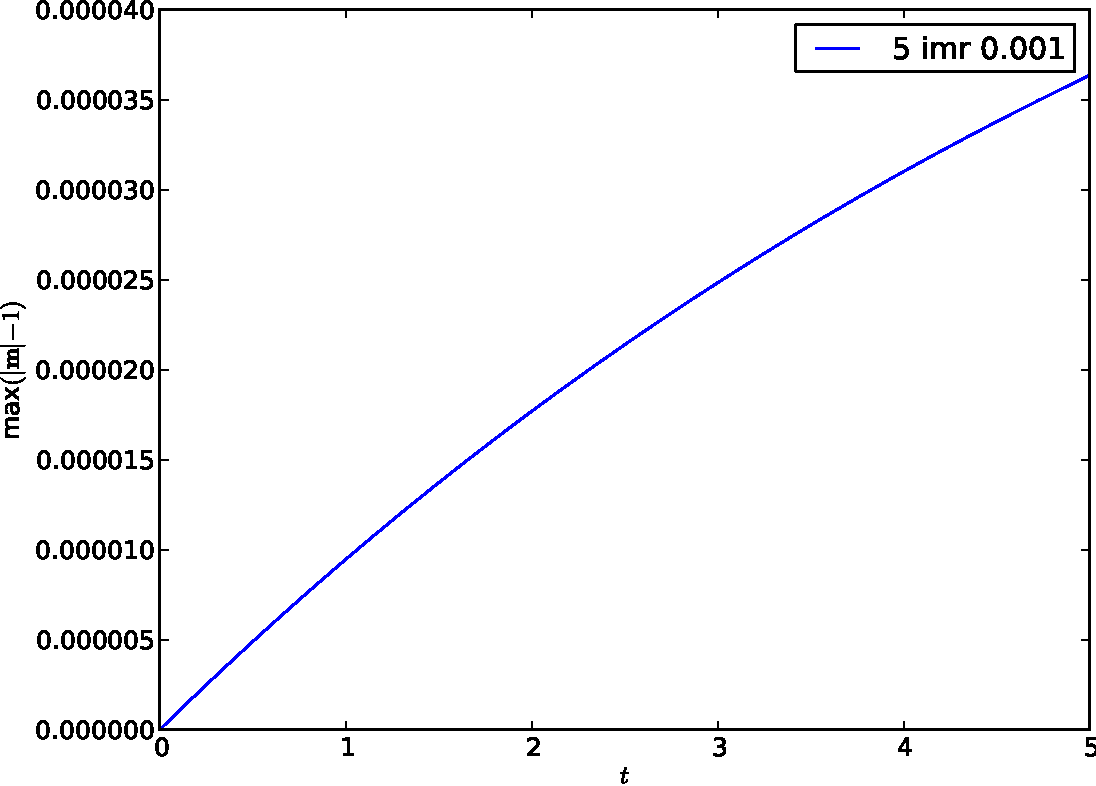
\includegraphics[width=0.8\textwidth]{plots/2d_wave_solution_m_length/gauss-maxmathbfm-1vst.pdf}
  \caption{Evolution of the maximum error of nodal magnetisation lengths in the 2D wave example with a standard Gaussian quadrature scheme.}
  \label{fig:mean-ml-error-2d-gauss}
\end{figure}

\begin{figure}
  \centering
  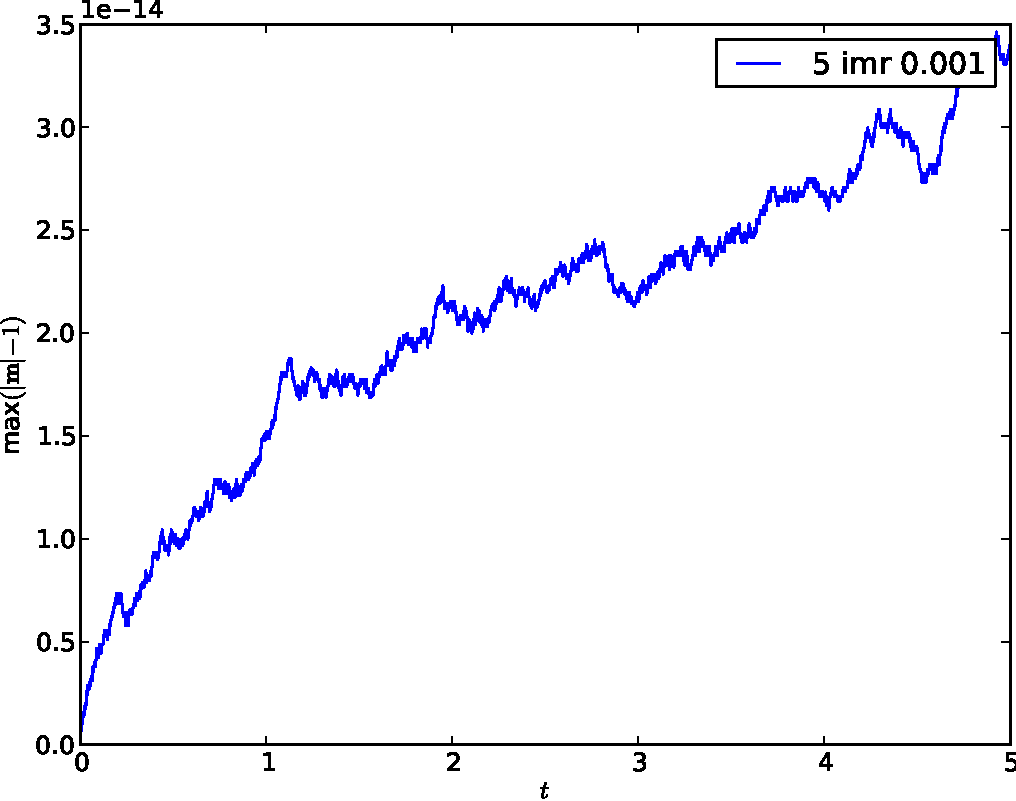
\includegraphics[width=0.8\textwidth]{plots/2d_wave_solution_m_length/lnodal-maxmathbfm-1vst.pdf}
  \caption{Evolution of the maximum error of nodal magnetisation lengths in the 2D wave example with the nodal quadrature scheme introduced above.}
  \label{fig:mean-ml-error-2d-nodal}
\end{figure}

To check that the conservation is independent of problem parameters we ran a parameter sweep using: square and triangle elements; 36, 441 and 6561 nodes; time steps of $0.1$, $0.01$ and $0.001$; and damping parameters of $1$, $0.1$, $0.001$ and $0$.
The maximum length error over all parameter sets, all time steps and all nodes when using nodal quadrature was 2.364775e-12, when using Gaussian quadrature it was 0.013746647.
This clearly demonstrates the necessity and effectiveness of the nodal quadrature scheme for retaining the conservation properties of the implicit midpoint rule.
% using the same data as for the figures above, look in their folders for parameter sets data parsing command: parse.py -d /mnt/moredata/optoomph/user_drivers/micromagnetics/experiments/parameter_sweeps/parameter_file_0/ -l=-dt -l=-damping --split=-integration --print-data max-max-ml --print-data ml -l=initial_nnode


??ds describe very long time behaviour in \cref{fig:mean-ml-error-2d-nodal-long-time}.

\begin{figure}
  \centering
  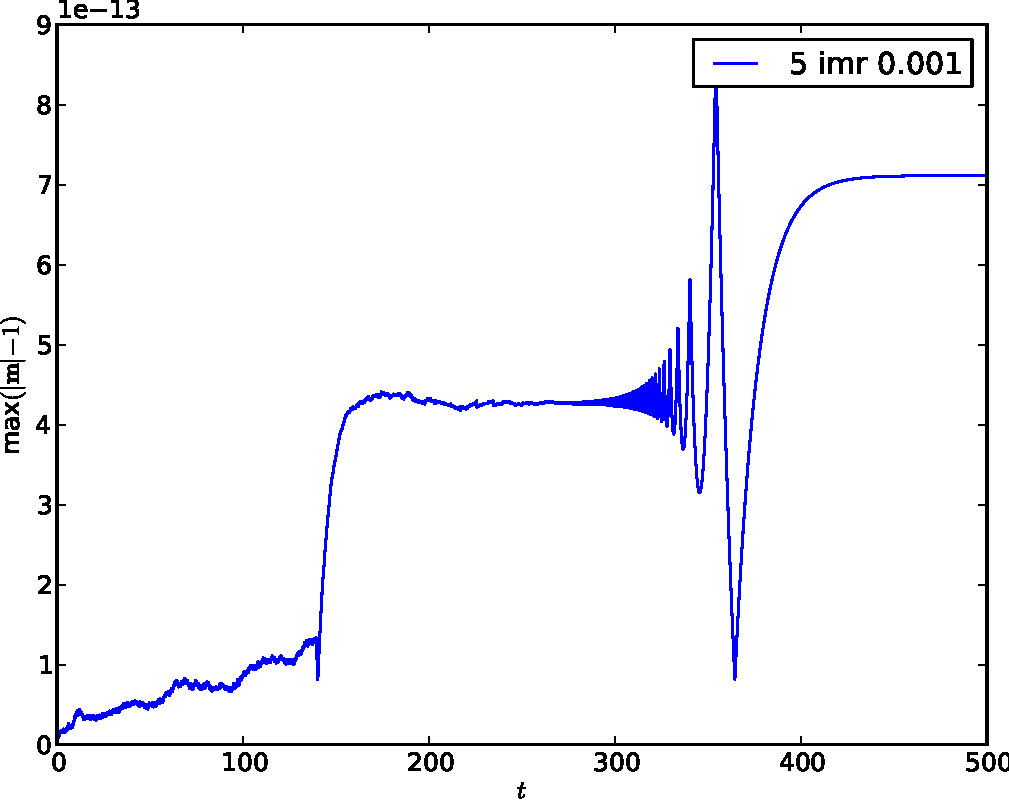
\includegraphics[width=0.8\textwidth]{plots/2d_wave_solution_m_length_long_time/-maxmathbfm-1vst.pdf}
  \caption{Evolution of the maximum error of nodal magnetisation lengths in the 2D wave example with the nodal quadrature scheme over a very long time period.}
  \label{fig:mean-ml-error-2d-nodal-long-time}
\end{figure}



\subsubsection{Effect of Newton tolerance}
\label{sec:effect-newt-toler-m-conservation}

Since the non-linear residual \cref{eq:weak-llg} used in the derivation of the conservation properties is only true up to the accuracy of the linearisation method we would expect to see some effect when modifying this accuracy.
In our model Newton's method is used for linearisation (see \cref{sec:newt-raph})so the relevant measure of accuracy is the Newton tolerance.

The obvious experiment to carry out would be to vary the Newton tolerance and examine how the error in $\abs{\mv}$ is affected.
However Newton's method extremely quickly meaning that the final residual is sometimes orders of magnitude smaller than the tolerance, this would hide any corrolation between the tolerance and the error.
Instead we plot the error against the actual maximum residual obtained (specifically: the mean over time steps of $\norm{\rv}_\infty$ after the Newton method has converged). 
The results are shown in \cref{fig:mean-ml-error-2d-nodal-newton-tests}, there is a clear corrolation between small residuals and small length errors.


\begin{figure}
  \centering
  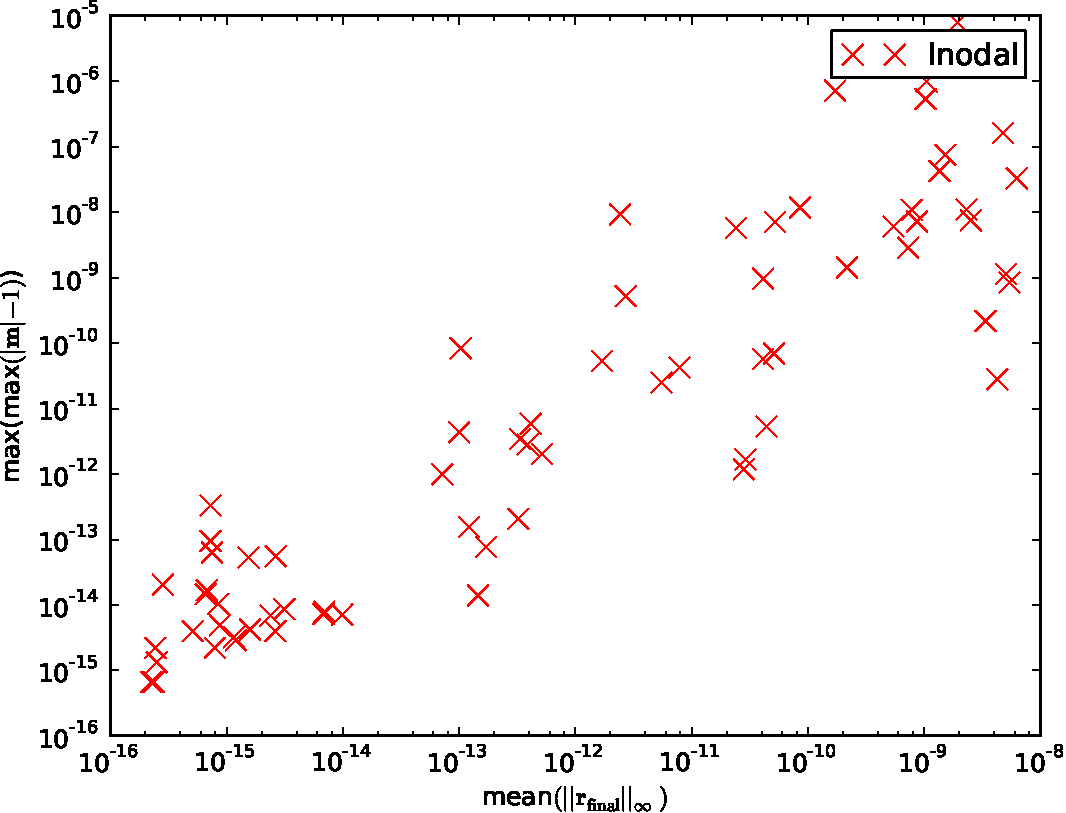
\includegraphics[width=0.8\textwidth]
  {plots/2d_wave_solution_m_length_newton_res/-maxmaxmathbfm-1vsmeanmathbfr_mathrmfinal_infty.pdf}
  \caption{Corrolation between maximum error of nodal magnetisation lengths and largest maximum Newton residual after convergence in the 2D wave example with the nodal quadrature scheme over a very long time period.}
  \label{fig:mean-ml-error-2d-nodal-newton-tests}
\end{figure}


% \subsubsection{Adaptivity}
% ??ds - no need for this? leave it to the final subsection?

% It remains to demonstrate that the adaptivity scheme introduced in \cref{sec:adaptive-imr} is effective for the finite element problem with nodal integration.
% Since there is still no relationship with previous time step sizes in the conservation proofs with nodal integration we don't expect there to be any issues with variable step size and conservation.

% Additionally our discretisation can be written as semi-discretisation in space (giving a system of ODEs) followed by the application of IMR in time.
% Hence we have no reason to expect the adaptive IMR to behave any differently to in the pure ODE case.

% \subsubsection{BEM}
% ??ds - no need for this? leave it to the final subsection?


% ??ds


\subsection{Conclusions}

??ds


%%% Local Variables:
%%% mode: latex
%%% TeX-master: "main"
%%% End:


\chapter{Hybrid Finite/Boundary Element Method}
\label{sec:hybr-finit-elem}
The hybrid finite/boundary element method works similarly to the normal finite element method except that one or more sub-regions are mapped onto their boundary \cite{Rammohan2002}.
The main advantage of this is that we reduce the dimensionality of these sub-regions one since we only have to solve equations on the boundary instead of the entire space.
In our case this is likely to give an advantage over a pure finite element method since we no longer need to mesh a long way outside the magnetic domain to accurately account for the effect of the external region. Also other methods for dealing with infinite domains can often give additional errors due to the truncation of the external domain.\cite{Bottauscio2008}

On the downside this mapping typically results in a dense matrix after discretisation, to which we cannot apply sparse matrix techniques.
Also the integrals that need to be computed may involve singularities, which introduce additional complications and may reduce accuracy or increase computation time.

Note that the derivation for this hybrid method comes from potential theory, rather than the boundary integral formulation usually used to construct the standard boundary element method.

\section{Derivation of the continuous problem}
\label{sec:bem-derivation}

\subsection{Background of the Method}
\label{sec:basic-method}
We want to use the boundary element method in the calculation of the magnetostatic scalar potential $\phim$, ($\hms = - \nabla \phim$), in the infinite region outside of a magnetic body.
Using the boundary element method directly, however, would require the solution of dense matrix equations for the entire problem.

We can circumvent this problem by splitting the potential into two parts $\phim = \phione + \phitwo$ in such a way that $\phione$ can be calculated the magnetic region(s) using only the finite element method.
We then have some conditions on $\phitwo$ that must be satisfied to give the correct total potential in $\magd$ and on $\boundd$, but, in order to solve for $\phitwo$ in the magnetic domain, we still need to find the boundary conditions (on the edge of the magnetic domain).
So we choose a charge distribution on the boundary that satisfies all the conditions on $\phione$ and $\phitwo$.
We can then solve for $\phitwo$ on the boundary using similar techniques to those used in the boundary element method.
Finally we apply the finite element method to find $\phitwo$ inside the magnetic region $\magd$.

By the uniqueness of solution for Poisson's equation with Dirichlet and/or Neumann boundary conditions we know that the field $ \hms = \nabla \phim$  constructed by the above steps is \emph{the} magnetostatic field.\footnote{To see this take the difference of two solutions of Poisson's equation: $\phi = \psi_1 - \psi_2$. Then using identity \eqref{eq:20}, the linearity of Poisson's equation and the divergence theorem we obtain $\int_S \phi \nabla \phi \cdot d \mathbf{S} = \int_V (\nabla \phi)^2 dV$. Applying Dirichlet, Neumann or mixed boundary conditions shows that the boundary integral is zero and hence $\nabla \phi = 0$.}

\subsection{Problem Description}
\label{sec:problem-description}
Let $\phim^\inte$ be the value of $\phim$ (with subscripts as appropriate) close to the boundary $\boundd$ and just inside the magnetic domain  and $\phim^\exte$ the value of $\phim$ just outside the magnetic domain\footnote{More precisely $\phim^\inte(\xv) = \lim_{\xv \rightarrow \boundd} \phim(\xv)$ from inside the magnetic domain, $\phim^\exte(\xv) = \lim_{\xv \rightarrow \boundd} \phim(\xv)$ from outside the magnetic domain.} (see \autoref{fig:BEM-geometry}).

We have the following \emph{physical} conditions\footnote{Equations~\eqref{eq:2}-\eqref{eqn:phibound} come from the definition of $\phim$, requirement for finite total energy, $\Bv^\text{int} \cdot \nv = \Bv^\text{ext} \cdot \nv$ and ??ds respectively.} on the total magnetostatic potential $\phim$:
\begin{equation}
  \lap \phim(\xv) = \nabla \cdot \mv(\xv) \qquad \forall \xv \in \magd \cup \extd,
  \label{eq:2}
\end{equation}
\begin{equation}
  \phim(\xv) \rightarrow 0 \qquad \text{ as } \abs{\xv} \rightarrow \infty,
\end{equation}
\begin{equation}
  \pd{\phim^\inte(\xv)}{\nv} - \pd{\phim^\exte(\xv)}{\nv} = \mv \cdot \nv \qquad \xv \in \boundd,
  \label{eqn:dphibound}
\end{equation}
\begin{equation}
  \phim^\inte(\xv) - \phim^\exte(\xv)  = 0 \qquad \xv \in \boundd.
  \label{eqn:phibound}
\end{equation}
Note that equations~\eqref{eqn:dphibound} and \eqref{eqn:phibound} imply continuity but not smoothness of the magnetic potential $\phim$ across $\boundd$. This is due to surface magnetic charges.

We choose $\phione$ to satisfy:
\begin{equation}
  \phim(\xv) = \phione(\xv) + \phitwo(\xv) \qquad \forall \xv \in \fulld,
  \label{eq:21}
\end{equation}
\begin{equation}
  \lap \phione(\xv) = \nabla \cdot \mv(\xv) \qquad \xv \in \magd,
  \label{eq:1}
\end{equation}
\begin{equation}
  \pd{\phione^\inte(\xv)}{\nv} = \mv \cdot \nv \qquad \xv \in \boundd,
  \label{eqn:dphionebound}
\end{equation}
\begin{equation}
  \phione(\xv) = 0 \qquad \xv \in \extd.
  \label{eqn:phioneoutside}
\end{equation}
Note that equations~\eqref{eq:1} and \eqref{eqn:dphionebound} give a self contained Poisson Neumann problem for $\phione \in \magd \cup \boundd$.

The equations~\eqref{eq:2} to \eqref{eqn:phibound} for $\phim$ combined with equations~\eqref{eq:21} to \eqref{eqn:phioneoutside} for $\phione$ give a number of conditions on $\phitwo$ must satisfy. Since the Laplacian operator is linear, \ie $\lap \phim = \lap \phione + \lap \phitwo$, from \eqref{eq:2} and \eqref{eq:1} it follows that
\begin{equation}
  \label{eq:8}
  \lap \phitwo(\xv) = 0 \qquad \forall \xv \in \fulld.
\end{equation}

Equation~\eqref{eqn:phioneoutside} implies that $\pd{\phione^\exte(\xv)}{\nv} = 0$. Combining this with equations \eqref{eqn:dphionebound} and \eqref{eqn:dphibound} gives
\begin{equation}
  \label{eq:5}
  \pd{\phitwo^\inte(\xv)}{\nv} - \pd{\phitwo^\exte(\xv)}{\nv} = 0.
\end{equation}

Finally from equations \eqref{eqn:phibound}, \eqref{eq:21} and \eqref{eqn:phioneoutside} we have
\begin{equation*}
  \phione^\inte - \phione^\exte + \phitwo^\inte - \phitwo^\exte = 0,
\end{equation*}
\begin{equation}
  \phitwo^\inte - \phitwo^\exte = - \phione^\inte.
\label{eq:4}
\end{equation}

\begin{figure}
  \center
  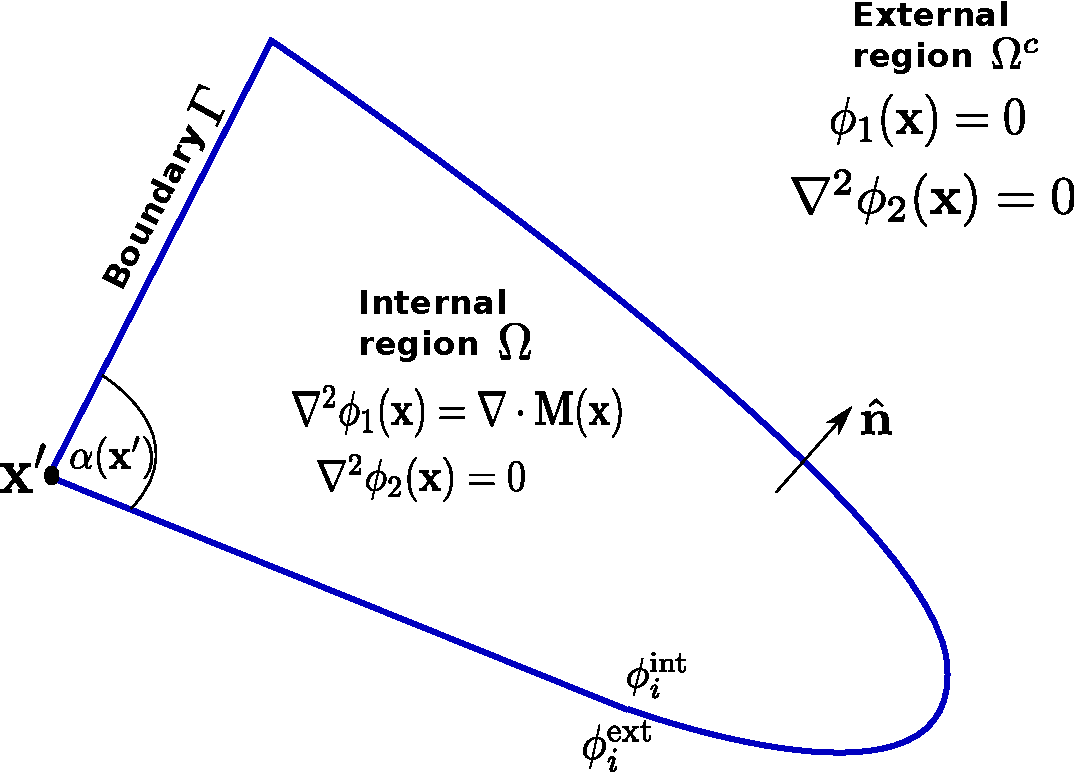
\includegraphics[width=0.75\textwidth]{./images/BEM-geometry}
  % \begin{tikzpicture}

  %   % Main nodes and some labels
  %   \node[label=below:$\xv'$] (a) at (-2,-2) {};
  %   \node (b) at (-2,2) {};
  %   \node[label=right:\Large{$\boundd$}] (c) at (5,0) {};

  %   % Draw main shape of magnetic domain
  %   \draw [line width=0.5mm,draw=solidblue,fill=paleblue] (a.north) to [bend right=71] (c) to (b.south);
  %   \draw [line width=0.5mm,draw=solidblue] (a) to (b);
  %   \draw (a.north) circle(1mm) [fill=black] {};

  %   % More labels
  %   \node (center) at (1,0) {\Large{Magnetic domain $\magd$}};
  %   \node(external) at (8,3) {\Large{External region $\extd$}};
  % \end{tikzpicture}

  \caption{A 2D representation of the geometry showing the labels used in this section. The point $\xv'$ is a singular point of the boundary $\boundd$, the angle $\alpha(\xv')$ is as shown.}
  \label{fig:BEM-geometry}
\end{figure}

\subsection{Double Layer Potentials}
\label{sec:double-layer-potent}
A double layer potential can be thought of as the potential due to a layer of dipoles of magnitude $\mu(\xv)$ in direction $\nv$ over the surface $S$.\cite{Sternberg1946} We will demonstrate that we can use a double layer potential to calculate $\phitwo^\inte$ in terms of $\phione^\inte$.

The double layer potential at a point $\xv \in \real^d$ is defined as \cite{eom_double_layer_potential}
\begin{equation}
  \label{eq:3}
  \phim(\xv) = \int_{S} \mu(\yv) \pd{\Green}{\nv(\yv)} \d \yv,
\end{equation}
where $G$ is the Green's function for a Laplacian operator.
For $d=2$
\[ \Green = \dfrac{-1}{2\pi}\ln(\abs{\xv - \yv}), \]
and for $d=3$
\begin{equation} \Green = \dfrac{-1}{4 \pi} \dfrac{1}{\abs{\xv - \yv}}.
  \label{eqn:greenslaplacian3d}
\end{equation}


We have the following results from potential theory:\cite{Sternberg1946}
\begin{enumerate}
\item The double layer potential satisfies Laplace's equation $\lap \phi = 0$ (in other words the double layer potential is harmonic).% pages ?

\item The double layer potential undergoes a jump of $\mu(\xv)$ moving in the direction $\nv$ across a smooth surface $S$, \ie
  \begin{equation}
    \label{eq:15}
    \phim^\inte(\xv) - \phim^\exte(\xv) = \mu(\xv).
  \end{equation}
% pages 136-140

\item For $\xv \in S$ the following relationship holds
  \begin{equation}
    \phim^\inte(\xv) = (1 - \frac{\alpha(\xv)}{\alpha_{\text{max}}}) \mu(\xv) + \phim(\xv),
    \label{eq:22}
  \end{equation}
  where $\alpha(\xv)$ is the angle (or solid angle) in two (or three) dimensions subtended by the domain at $\xv$ and
\begin{equation*}
  \alpha_{\text{max}} =
  \begin{cases}
    2 \pi & \text{if } d=2 \\
    4 \pi & \text{if } d=3.
  \end{cases}\label{eq:16}
\end{equation*}
Note that $\alpha(\xv)$ is the angle at the exact point $\xv$, when the surface at $\xv$ is a Lyapunov surface (\ie not a sharp corner) $\frac{\alpha(\xv)}{\alpha_{\text{max}}}$ reduces to a factor of $1/2$. We write $\gamma(\xv) = \frac{\alpha(\xv)}{\alpha_{\text{max}}}$ for simplicity.
 % pages 137-139, page 155 for 2d

\item If $\mu$ is continuous and has continuous first and second derivatives along the boundary (\ie $\mu(\xv) \in C^2[S]$) then the limits $\pd{\phim^\inte(\xv)}{\nv}$ and $\pd{\phim^\exte(\xv)}{\nv}$ exist and are equal. % pages 145-153.

\end{enumerate}

Some notes on the derivation of the above results in Sternberg 1946\cite{Sternberg1946}:
\begin{itemize}
\item Some derivations of the results above rely on the surface being a ``Lyapunov surface'' which imposes a number of smoothness conditions, in particular excluding surfaces with corners.
The proofs given in Sternberg allow a finite number of sharp corners, \ie a polygonal domain.
\item Our potentials are a factor of $\frac{-1}{4 \pi}$ different from those in the reference. Also our $\phim^\inte$ and $\phim^\exte$ definitions correspond respectively to $\phim^-$ and $\phim^+$ in the book.
\end{itemize}

\subsection{Application to Magnetostatic Calculations}
\label{sec:appl-magn-calc}

From \autoref{sec:double-layer-potent} we can see that conditions \eqref{eq:8}, \eqref{eq:5} and \eqref{eq:4} on $\phitwo$ are satisfied by a double layer potential with magnitude
\begin{equation}
  \label{eq:24}
  \mu(\xv) = - \phione^\inte(\xv).
\end{equation}

By the uniqueness of solution for Poisson's equation this gives us, up to an additive constant, the only solution for $\phitwo(\xv)$ in the external region.
This is good enough for a potential since it is only used in $\hms(\xv) = - \nabla \phim(\xv)$ so addition of a constant has no effect.

From equations~\eqref{eq:3}, \eqref{eq:22} and \eqref{eq:24} we have:
\begin{equation}
  \label{eq:6}
  \phitwo^\inte(\xv) =  \big(\gamma(\xv) - 1 \big) \phione^\inte(\xv)
  - \int_{\boundd} \phione^\inte(\yv) \pd{\Green}{\nv(\yv)} \d \yv.
\end{equation}
After substituting in our definition for the three dimensional Green's function \eqref{eqn:greenslaplacian3d} we obtain the same equation as given by Koehler \cite{Koehler1997}.
Similar equations are solved when using the standard boundary element method, hence the name.

Also note that $\phim = \phione + \phitwo$ everywhere and so
\begin{align}
  \label{eq:18}
  \phim^\inte(\xv) &= \bm \big[ \phione^\inte(\xv) \big] \\
  &= \gamma(\xv) \phione^\inte(\xv)
  - \int_{\boundd} \phione^\inte(\yv) \pd{\Green}{\nv(\yv)} \d \yv. \notag
\end{align}

Either equation~\eqref{eq:6} or \eqref{eq:18} can be used to give boundary conditions for $\phitwo \in \magd$ or $\phim \in \magd$ respectively. We will proceed using equation~\eqref{eq:18} for simplicity since it eliminates $\phitwo$ from later calculations.

Hence, given the solution for $\mv(\xv) \in \magd$ the complete continuous problem is
 \begin{subequations}
   \label{eq:phi-bem-continuous}
   \begin{align}
     \label{eq:phim-bem-continuous}
     \lap \phim(\xv) &= \div \mv(\xv) \quad & \xv \in \magd, \\
     \label{eq:phi1-bem-continuous}
     \lap \phione(\xv) &= \div \mv(\xv)    & \xv \in \magd,
   \end{align}
 \end{subequations}
with boundary conditions
 \begin{subequations}
   \label{eq:phi-bem-continuous-bc}
   \begin{align}
     \label{eq:phim-bem-continuous-bc}
     \phim(\xv) &= \bm \big[ \phione(\xv) \big]      & \xv \in \boundd, \\
     \label{eq:phi1-bem-continuous-bc}
       \pd{\phione(\xv)}{\nv} &= \mv \cdot \nv  & \xv \in \boundd.
   \end{align}
 \end{subequations}
Here we have dropped the distinction between $\inte$ and $\exte$ since all exterior values have been eliminated.


\section{Discretisation}
\label{sec:discretisation}

The bulk equations~\eqref{eq:phi-bem-continuous} and the boundary condition on $\phione$, equation~\eqref{eq:phi1-bem-continuous-bc}, are identical to those discussed in \autoref{sec:llg-initial-equations}.
As such the weak residual form, discretisation and Jacobian calculations are identical for these equations.
Therefore all that remains to be discretised is the operator $\bm$. We let
\begin{equation}
  \phim = \sum_\ibasis \phim_{\ibasis} \tbf_{\text{m},\ibasis}(\xv),
  \qquad
  \phione = \sum_\ibasisb \phione_{\ibasisb} \tbf_{1,\ibasisb}(\xv),
  \label{eq:25}
\end{equation}
where $\tbf_\ibasis(\xv_\ibasisb) = \delta_{\ibasis \ibasisb}$ on the boundary nodes and is linearly interpolated from $\tbf_\ibasis = 1$ at $\xv_\ibasis$ to $\tbf_\ibasis = 0$ at neighbouring nodes.

Substituting equations~\eqref{eq:25} into \eqref{eq:18} we have
\begin{equation*}
  \sum_\ibasis \phim_{\ibasis} \tbf_{\text{m},\ibasis}(\xv) =
  - \int_{\boundd} \sum_\ibasisb \phione_{\ibasisb} \tbf_{1,\ibasisb}(\yv)
  \pd{\Green}{\nv(\yv)} \d \yv
  \quad + \gamma(\xv) \sum_\ibasisb \phione_{\ibasisb} \tbf_{1,\ibasisb}(\xv).
\end{equation*}

To get the value of $\phim$ at node $\ibasisc$ we choose $\xv = \xv_\ibasisc$. Then using the property $\tbf_\ibasis(\xv_\ibasisc) = \delta_{\ibasis \ibasisc}$ and replacing $\ibasisc$ by $\ibasis$ we have
\begin{equation}
  \phim_{\ibasis} =
  - \int_{\boundd_\ibasisb} \sum_\ibasisb \phione_{\ibasisb} \tbf_{1,\ibasisb}(\yv)
  \pd{\Green[\ibasis]}{\nv(\yv)} \d \yv
  \quad + \gamma(\xv_\ibasis) \phione_{\ibasis},
  \label{eq:colocation}
\end{equation}
where ${\boundd_\ibasisb}$ is the region where $\tbf_{1,\ibasisb} \neq 0$, \ie the elements which contain node $\ibasisb$.

Finally, since the integrands are continuous functions ??ds citation needed, we can move the sum outside the integral leaving
\begin{equation}
  \phim_{\ibasis} =
  - \sum_\ibasisb \phione_{\ibasisb} \Big[ \int_{\boundd_\ibasisb} \tbf_{1,\ibasisb}(\yv)
  \pd{\Green[\ibasis]}{\nv(\yv)} \d \yv \Big]
  \quad + \gamma(\xv_\ibasis) \phione_{\ibasis}.
\label{eq:27}
\end{equation}
Notice that the expression inside the square brackets is independent of all the potentials: it depends only on the geometry and so can be pre-calculated and stored in many cases.

So equation~\eqref{eq:27} gives $\phim$ at a boundary node in terms of a sum of geometric factors multiplied by $\phione$ at each boundary node.
In other words, this is a dense matrix multiplication by a pre-computed matrix giving $\phim$ at all the boundary nodes in terms of $\phione$ at all boundary nodes:
\begin{equation}
  \label{eq:10}
  \phim_\ibasis = \bm_{\ibasis,\ibasisb} \cdot \phione_{\ibasisb},
\end{equation}
where
\begin{equation}
  \label{eq:17}
  \bm_{\ibasis\ibasisb} = - \int_{\boundd_\ibasisb} \tbf_{1,\ibasisb}(\yv) \pd{\Green[\ibasis]}{\nv(\yv)} \d \yv
  \quad + \gamma(\xv_\ibasis)\delta_{\ibasis\ibasisb}.
\end{equation}


% ??ds wrong place for this discussion and not sure if integral is really singular or not due to the n.r term...
%Note that although this integral appears at first glance to be singular when the node $\xv_\ibasis$ is within $\boundd_\ibasisb$ (the line segment or section of surface being integrated over)
%A benefit of this is that the matrix is always well conditioned because the largest terms are near the singularity and hence near the diagonal elements $\ibasisb = \ibasis$.
%However the singularity can cause difficulties in the evaluation of the affected integrals.
%Methods to overcome these difficulties are discussed in the next section.

We now convert the normal derivative of the Green's function into a more tangible form.
In 3D
\begin{equation}
  \label{eq:11}
  \pd{\Green}{\nv} = \frac{-1}{4 \pi} \pd{}{\nv} \Gthreed = \frac{-1}{4 \pi} \nv \cdot \nabla \Big( \Gthreed \Big).
\end{equation}
Converting to spherical coordinates with the origin at $\xv$ ($r = \abs{\yv - \xv}$, $\ruv = \frac{\yv - \xv}{r}$) we have\footnote{In spherical polar coordinates $\nabla = \ruv \pd{}{r} +  \phiv \frac{1}{r} \pd{}{\phi} + \thetav \frac{1}{r \sin \theta} \pd{}{\theta}$. Obviously $\frac{1}{r}$ has no angular dependence so only the derivative with respect to $r$ is non-zero.}
\begin{equation}
  \label{eq:12}
  \pd{G(r)}{\nv} = \frac{-1}{4 \pi} \nv \cdot \ruv \pd{}{r} \Big( \frac{1}{r} \Big)
  = \frac{+1}{4 \pi}  \frac{\nv \cdot \ruv}{r^2},
\end{equation}
\begin{equation}
  \label{eq:13}
  \pd{\Green}{\nv} = \frac{\nv \cdot (\yv - \xv)}{4 \pi \abs{\yv - \xv} ^2} .
\end{equation}
Similarly in 2D we find
\begin{equation}
  \label{eq:14}
  \pd{\Green}{\nv} = \frac{-1}{2 \pi} \pd{}{\nv} (\Gtwod) = \frac{\nv \cdot (\yv - \xv)}{2 \pi \abs{\yv - \xv}}.
\end{equation}

So the discretised boundary element matrix in $d=2,3$ dimensions is
\begin{equation}
  \label{eq:19}
  \bm_{\ibasis\ibasisb} =\frac{-1}{2^{(d-1)} \pi} \int_{\boundd_\ibasisb} \tbf_{1,\ibasisb}(\yv) \frac{\nv(\yv) \cdot (\yv - \xv_\ibasis)}{\abs{\yv - \xv_\ibasis} ^{d-1}} \d \yv
   \quad + \gamma(\xv_\ibasis)\delta_{\ibasisb\ibasis}.
\end{equation}
We denote the integral in this equation by $I_\bm$.

\subsection{Discretisation Approaches: Co-location vs Galerkin}

In deriving equation~\eqref{eq:colocation} we used a co-location approach rather than the Galerkin approach used in our FEM method.
The reason for this choice is that a Galerkin discretisation would lead to a double integral over the boundary, which would probably be more difficult to calculate.

Not sure what effect this has, if any, on the stability or accuracy of the scheme...

\section{Evaluation of the discrete boundary operator}
\label{sec:calc-integr-i_bm}

\section{Singularity of the main integral}
\label{sec:bem-singularity}

Another factor that should be considered is the apparent singularity in the integral $I_\bm$ when integrating over an element containing the source point $\xv_\ibasis$. There are two distinct cases to look at here: flat elements and curvilinear elements.

In the case of flat elements if $\xv_\ibasisb$ is within the element being integrated over then we have
\begin{equation}
  \label{eq:7}
  \nv(\yv) \cdot \ruv_{\xv_{\ibasis} \rightarrow \yv} \equiv 0 \quad \forall \yv \in \text{element}.
\end{equation}
So the integral is zero and the singularity is avoided. Unfortunately for neighbouring elements this is not necessarily true--in particular elements at a sharp corner may be very close to a node where $\nv(\yv) \cdot \ruv_{\xv_{\ibasis} \rightarrow \yv} \neq 0$ resulting in a near-singular integral.

For curvilinear elements we no longer have the nice property that any potentially singular elements are automatically zero. However it can be shown that for reasonably shaped elements ??ds citation needed! there are still no real singular integrals only near-singular ones. This is due to the fact that $\nv(\yv) \cdot \ruv_{\xv_{\ibasis} \rightarrow \yv}$ tends to zero ``faster'' than $\abs{\yv - \xv_\ibasis}^2$ so the limit of the ratio as $\yv \rightarrow \xv_\ibasis$ is zero. In fact integrals like this are routinely evaluated in standard boundary element methods ??ds citation needed.


\subsection{Corner Singularities}

Have to handle calculation of angles/solid angles $\gamma(\xv)$ somehow.

So far I've just assumed the information will be provided

Inderpretations: only count ``real'' sharp corners (\ie sphere has no corners) vs include all element corners (\ie sphere has sharp corners at every element join).


\subsection{Analytical solutions}

??ds you need to thoroughly check the maths in this section at least once more

For linear shape functions and triangular elements an exact analytical solution for the singular integral $I_G$ was given by Lindholm \cite[App. B]{Lindholm1984}.\footnote{Note: Lindholm's definition of the 3d Green's function is a factor of -1 different to ours.}. 
Combining equations (2) and (3) from \cite{Lindholm1984} with equation~\eqref{eq:13} and using our notation for positions, we see that Lindholm's $L$ operator is
\begin{equation}
  \begin{aligned}
    L[U] &= \frac{-1}{4 \pi}\int_\boundd U(\yv) \frac{\nv(\yv) \cdot (\yv -
      \xv)}{\abs{\xv - \yv}^2}
    \d\yv, \\
    &= -G[U] + \gamma(\xv) U(\xv).
  \end{aligned}
\end{equation}
So $L[\tbf_{1,\ibasisb}]$ integrated over the surface triangle $\boundd_\ibasisb$ with $\xv = \xv_\ibasis$ corresponds exactly to the integral $I_{G,i,j}$ required in the calculation of $G_{i,j}$\footnote{The minus sign from the different definitions of the Green's function has cancelled with the minus sign from the fact that we are interested in calculating $-1$ times the operator.}.

To clearly see the equivalence between the discretised operators we need to go through both discretisations simultaneously.
Ignoring sharp corners we have that
\begin{equation}
  \begin{aligned}
    \phim(\xv) = G[\phione](\xv) &= -L[\phione](\xv), \\
    %
    \sum_{n} \phim_n \tbf_n(\xv) 
    &= - \sum_{\tri=1}^{N_\tri} \sum_{i=1}^{3} L_{\tri,i}(\xv) \phione_{\tri,i}, 
    \quad\quad&\text{expand}\\
    % 
    \sum_{n} \phim_n \tbf_n(\xv) 
    &= - \sum_{\tri=1}^{N_\tri} \sum_n L_{\tri,n}(\xv) \phione_n, 
    &\text{equivalent to sum over all nodes--local support}\\
    % 
    \phim_k &= - \sum_{\tri=1}^{N_\tri} \sum_n L_{\tri,n}(\xv_k) \phione_n, 
    &\text{use $\tbf_n(\xv_k) = \delta_{nk}$}\\
    % 
    \phim_k &= \sum_n \bigs{\sum_{\tri=1}^{N_\tri} -L_{\tri,n}(\xv_k)} \phione_n, 
    &\text{reorder}\\
    %
    \phim_k &= \sum_n \bigs{\sum_{\tri \in \text{around}(n)} -L_{\tri,n}(\xv_k)} \phione_n,
    &\text{reduce elements to sum over--local support again}\\
    %
    &= \sum_n G_{k,n} \phione_n. 
    &\text{equation~\eqref{eq:10}}
  \end{aligned}
\end{equation}
Therefore 
\begin{equation}
  IG_{i,j} = \sum_{\tri \in \text{around}(j)} L_{\tri,k}(\xv_i),
\end{equation}
where $k$ is the index of node $j$ within triangle $\tri$.

Let
\begin{equation}
  \begin{aligned}
    \rv_k(\xv) &= \zv_k - \xv, &\quad \text{(vector from triangle node $k$ to $\xv$)} \\
    \sv_k &= \zv_{k+1} - \zv_k, & \text{(vector along an edge of the triangle)} \\
  \end{aligned}
\end{equation}
and let $\hat{\sv}$, $\hat{\rv}$ be the equivalent unit vectors.
Hence using the third (un-numbered) equation in appendix B of \cite{Lindholm1984}, converting to our notation and substituting in values from the rest of appendix B where practical we have
\begin{equation}
  \begin{aligned}
    \label{eq:analytic-bem-integral}
    I_{G,i,j} &= \sum_{\tri \in \text{around}(j)} \frac{\abs{\sv_{k+1}}}{8 \pi A_\tri} \bigb{
      \bigb{(\nv_\tri \times \hat{\sv}_{k+1}) \cdot \rv_{k+1}(\xv_i)} \Omega_\tri(\xv_i) 
      - \nv_\tri \cdot \rv_1(\xv_i) \sum_{l=1}^{3} (\hat{\sv}_{k+1} \cdot \hat{\sv}_l) P_l(\xv_i)
    }, \\
  \end{aligned}
\end{equation} 
where $A_\tri$ is the area of the triangle, $\zv_i$ denote the nodes of triangle $\tri$ (mod 3), and $\nv_\tri$ is the unit normal to the triangle. 
The quantity $P_l(\xv)$ is given by
\begin{equation}
  P_l(\xv) = \ln\bigb{\frac{\abs{\rv_l(\xv)} + \abs{\rv_{l+1}(\xv)} + \abs{\sv_l}}
    {\abs{\rv_l(\xv)} + \abs{\rv_{l+1}(\xv)} - \abs{\sv_l}}}.
\end{equation}
Finally we need $\Omega_\tri$, the solid angle subtended by the triangle at $\xv_i$:
\begin{equation}
  \label{eq:bem-triangle-solid-angle}
  \Omega_\tri(\xv) = \text{sign}(\nv_\tri \cdot \rv_1) 2 \cos^{-1}\bigs{\frac
    {\abs{\rv_1}\abs{\rv_2}\abs{\rv_3} + \abs{\rv_1} \rv_2\cdot\rv_3 + \abs{\rv_2}\rv_1\cdot \rv_2}
    {\sqrt{2(\abs{\rv_2}\abs{\rv_3} + \rv_2\cdot\rv_3)
        (\abs{\rv_3}\abs{\rv_1} + \rv_3\cdot\rv_1)
        (\abs{\rv_1}\abs{\rv_2} + \rv_1\cdot\rv_2)}}},
\end{equation}
where we have dropped the $\xv$ argument from $\rv_i(\xv)$ for brevity.
The use of $\rv_1(\xv)$ in equations~\eqref{eq:analytic-bem-integral} and \eqref{eq:bem-triangle-solid-angle} is not a typo: the results are independant of which node in the triangle is used.


A useful open source implementation of this calculation in \texttt{C} is included in \texttt{magpar}\cite{magpar-website} and redistributed in \texttt{nmag}\cite{nmag-website}.


\subsubsection{Numerical integration}

The analytical formula given in the previous Section is fast and accurate when applicable but also greatly limits the allowed meshes.
It is very useful when testing code to be able to run 2D simulations, since the run time can be orders of magnitude smaller.
It is also sometimes useful to be able to use structured quadrilateral meshes for simple geometries and for testing purposes.
??ds higher order elements?
Both of these approaches are impossible with the analytical formula above.
It is likely that similar analytical results could be derived for each of these cases, but it is simpler and more general to use a numerical approach instead.

As discussed in \autoref{sec:bem-singularity} the integral $I_G$ is non-singular, so no special techniques are needed for its integration (other than what is needed to attain good accuracy).
As such an adaptive quadrature method can effectively calculate the integrals.
Our algorithm is roughly as follows:
\begin{enumerate}
\item Calculate the integral twice with different orders of quadrature.
\item If the difference is less than some tolerance then accept the result.
\item Otherwise repeat the calculation with a higher order quadrature, and goto 2.
\end{enumerate}

Alternate adaptivity process: use h-refinement instead/as well (divide integral into chunks). ??ds did I consider this?

Ideally we would like to include the calculations at lower order quadratures in the higher order ones, therefore use ??ds Clenshaw-Curtis quadrature\cite{Trefethen2008}.

Rapid increase in quadrature order to avoid wasting time calculating many intermediate attempts.

Formulae from ??ds.

Potentially problems could arise when $\xv_i$ is extremely close to the surface element, but not in the same plane (so that $\nv \cdot \rv \neq 0$).
This would occur, for example, in extremely thin or extremely sharp regions of magnetic material.
Such regions are unlikely to be a problem in practice because sufficiently thin/sharp domains are likely to be outside the scope of micromagnetism in general.



%%% Local Variables:
%%% mode: Latex
%%% TeX-master: "main"
%%% End:


\chapter{Efficient solution of the linear systems}
\chaptermark{Solution of linear systems}
\label{sec:solution-strategies}

When we apply implicit time integration schemes, a FEM spatial discretisation and the Newton-Raphson method for linearisation (as discussed in \cref{sec:time-discretisation,sec:galerk-meth-llg}) to the LLG equation we are left with the problem of solving a sequence of large sparse linear systems to obtain the approximate solution.
With the addition of FEM/BEM for calculation of magnetostatic fields (as discussed in \cref{sec:hybr-finit-elem}), the linear systems to be solved become larger and more complex.
In this \thisref{sec:solution-strategies} we discuss solution strategies for these systems.

In \cref{sec:llg-only-system} we first discuss the solution of the systems required in the calculation of the magnetostatic field assuming the magnetisation is known.
We then discuss methods of solving the linear systems for the LLG equation assuming the magnetostatic field is known.
This is non-trivial because of the inclusion of the dense BEM matrix.

In \cref{sec:solut-coupl-syst} we describe two efficient methods for the solution of the LLG equation with magnetostatics: a ``monolithic'' (\ie fully coupled) approach and a semi-implicit approach.
The semi-implicit approach breaks the problem into a sequence of easily solved linear systems but at the cost of modifying the time integration scheme.
The monolithic approach uses efficient iterative methods to solve the full linear system and preserves all properties of the time integration scheme, such as stability and geometric integration properties.
In particular the energy conservation property of IMR requires the use of a monolithic approach (see \cref{sec:proof-energy-prop}).
Except for the simplest preconditioner, \cref{eq:90}, the preconditioners for the monolithic approach are novel.

Finally, in \cref{sec:numer-exper-fem-bem-systems}, we present some numerical experiments demonstrating the effectiveness of the proposed linear solvers for the systems resulting from both the semi-implicit and monolithic approaches.



\section{Solution of decoupled systems}
\label{sec:llg-only-system}

In \thisref{sec:llg-only-system} we consider the solution of the magnetostatic and LLG problems in isolation (\ie the LLG problem is solved assuming that the magnetostatic field is a known function and vice-versa).
Such methods are important building blocks for the solution of the coupled system.

Firstly we consider the two linear systems solved in the magnetostatic field calculations: these are both Poisson systems (see \cref{eq:phi-bem-continuous} and \cref{eq:poisson-jacobian}), which are well studied.
One efficent and robust method for solving Poisson systems on unstructured grids is to use the method of conjugate gradients (CG) with algebraic multigrid (AMG) as a preconditioner \cite{Henson2002}.

Note that the matrices involved in the Poisson systems do not depend on $\phim$, $\phione$ or $\mv$ (\ie the Poisson problems are linear).
This means that when solving these parts of the problem the Newton-Raphson iteration is not required (or if used it will converge in a single iteration assuming that the linear solve is sufficiently accurate).
Also the Poisson matrices only depend on the geometry and so can be computed once and stored for reuse throughout the duration of the simulation (and similarly for the coarsening information required by the AMG preconditioner).


Now we focus on the sequence of linear systems resulting from solving the LLG equation with the Newton-Raphson method, \cref{eq:llg-jacobian}.
There do not appear to be any solvers which are efficient, robust and scale optimally with matrix size in the literature.
We try two solvers in our implementation, unfortunately neither are expected to be efficient for large matrix sizes and large time steps.

The first method used is a direct solve by LU decomposition.
As discussed in \cref{sec:direct-methods} this method is extremely robust but is very slow for large matrices, particularly for problems in three spatial dimensions.

The second method is to use a Krylov solver preconditioned by an incomplete LU decomposition (ILU), inspired by \cite{Suess2002}.
This method is expected to be efficient for medium sized problems and/or small time steps, especially in 2D or thin film problems where the FEM nodes are less coupled.
However the effectiveness is strongly dependent on the diagonal dominance of the matrix.
As the volume of the elements decreases or the time step size increases the matrix becomes less diagonally dominant and the effectiveness of the preconditioner will decrease.
Hence this method is not expected to scale optimally to fine meshes or to be very robust with respect to varying parameters.
This method is used by both \nmag \cite{fangor-in-viva} and \magpar.\footnote{See \texttt{src/llg/precond.c} line 271 in the \magpar version 0.9 source code.}

\section[Solution of the coupled system]{Solution of the coupled LLG-magnetostatics system}
\label{sec:solut-coupl-syst}

We now consider the solution of the combined LLG and FEM/BEM magnetostatics system.
Unlike typical FEM computations, these linear systems are not entirely sparse: the BEM matrix, $\bm$, (derived in \cref{sec:discretisation}, \cref{eq:17}) appears as a dense block in the Jacobian.
In this \thisref{sec:solut-coupl-syst} we describe two approaches to efficiently solve the resulting non-linear system despite this issue.

In \cref{sec:semi-implicit-bem} we describe the first approach which involves replacing our implicit time integration scheme with an ad-hoc semi-implicit version which handles the magnetostatic calculation explicitly.
This means that only decoupled solves for $\phione$, $\phi$ and $\mv$ are required at each time step, and the dense block, $\bm$, only appears as a matrix-vector multiply.
However it also means that we are no longer using the time integration methods discussed in \cref{sec:some-implicit-time-integrators}, instead we are using some new scheme.

The second approach, described in \cref{sec:fully-implicit-bem}, is to construct a linear solver which can efficiently handle the dense block.
We present a novel solver which consists of a Krylov solver combined with a preconditioner and an efficient representation of the BEM block.
This approach has the benefit that all of the properties of the original time integration schemes carry over to the coupled problem.
In particular when using this approach the IMR retains the energy property described in \cref{sec:proof-energy-prop}, which is the most interesting of its geometrical integration properties.\footnote{A number of integration schemes can obtain length conservation: Cayley transform methods \cite{Lewis2003}, semi-analytical methods \cite{Wiele2010} and various types of semi-implicit midpoint rule methods \cite{Spargo2003,Serpico2001,Mentink2010} (including the one described in \cref{sec:semi-implicit-bem}).}
Additionally it may be useful for stochastic problems (\ie when thermal fields are involved, see \cref{sec:temperature-effects}), since in this case only a few time integration schemes are known to converge to the correct solution.
The implicit midpoint rule is one of these schemes, but any semi-implicit modification is likely to remove this property \cite{DAquino2006}.

Before describing these approaches in more detail, we briefly discuss the implementation of the monolithic coupling between the LLG and magnetostatic problems, and the structure of the resulting Jacobian.

\subsection{Residuals and Jacobian for the monolithically coupled system}
\label{sec:bem-jacobian-structure}

As mentioned in \cref{sec:discretisation} the pair of potentials used in the FEM/BEM method is similar to that of the simplified magnetostatic potential discussed in \cref{sec:galerk-meth-llg}.
There are two differences: the first is that there is no coupling from the auxiliary potential $\phione$ to the LLG equation, and hence no corresponding block in the full Jacobian.

The second difference is that there is an additional coupling between the boundary values of $\phione$ and the boundary values of $\phim$.
This coupling between the BEM part (a collocation method) and the FEM part (a Galerkin method) is implemented using the following residual vector:
\newcommand{\rphimb}{\rphi_\boundd}
\begin{equation}
  \rphimb(\phimdis_\boundd, \phionedis_\boundd) = \bm \phionedis_\boundd - \phimdis_\boundd,
  \label{eq:89}
\end{equation}
where $\mydiscrete{x}_\boundd$ denotes the vector of values of $x$ at the boundary nodes.
This residual is included as normal in the non-linear solve and simply enforces the condition $\phimdis_\boundd = \bm \phionedis_\boundd$ from \cref{eq:10}.
Note that we cannot enforce the condition in the standard way for Dirichlet boundary conditions (by pinning the values at the boundary nodes to the appropriate values) because the condition is obtained as part of the solve.

A natural consequence of \cref{eq:89} is that the BEM matrix is a block of the Jacobian:
\begin{equation}
  \pd{\rphimb}{\phionedis_\boundd} = \bm,
  \label{eq:92}
\end{equation}
where we have again used the notation that $\pd{\av}{\bv}$ is the Jacobian of the derivatives of $\av$ with respect to $\bv$, as in \cref{eq:jac-def}.
Also note that the diagonal Jacobian block for the boundary values of $\phim$ is simply the negative of the identity matrix
\begin{equation}
  \pd{\rphimb}{\phimdis_\boundd} = -\Idm.
  \label{eq:91}
\end{equation}

\newcommand{\Amm}{\Am_\phim}
\newcommand{\Amu}{\Am_\phione}
\newcommand{\zm}{0}
\newcommand{\Abound}{\Am_{\phim\boundd}}

\newcommand{\scalemath}[2]{\scalebox{#1}{\begin{math} {#2} \end{math}}}

\newcommand{\Aprime}{\scalemath{0.5}{\begin{matrix} \Amm     & \Abound \\ \zm      & -\Idm \end{matrix}}}
\newcommand{\Gprime}{\scalemath{0.5}{\begin{matrix} \zm  & \zm \\ \zm  & \bm \end{matrix}}}
\newcommand{\Qprime}{\scalemath{0.5}{\begin{matrix} \Qm \\ \zm \end{matrix}}}


Combining the above with the Jacobian matrix as derived in \cref{sec:llg-magn-coupl}, the complete Jacobian is
\begin{equation}
  \Jm =
  \scalemath{2}{
    \begin{pmatrix}
      \Fm        & \Pm     &  \zm \\
      \Qprime &   \Aprime &  \Gprime  \\
      \Qm       &  \zm       &   \Amu
    \end{pmatrix}
  },
  \label{eq:16}
\end{equation}
where $\Abound = \pd{\phimh}{\phimdis_\boundd}$ is the Jacobian of the bulk $\phim$ values with respect to the boundary values.
The order of blocks is $\mv$, $\phim$, $\phione$.
The blocks corresponding to derivatives of the $\phim$ residual are broken into sub-blocks for the bulk and boundary values due to the BEM coupling.
The overall Jacobian is a square matrix with number of rows $\nrow = 5\Nn$, where $\Nn$ is the number of nodes.
The LLG block, $\Fm$, is of size $3\Nn\times 3\Nn$, the Poisson block, $\Amu$, is of size $\Nn \times \Nn$.
The smaller Poisson block, $\Amm$, is of size $\Nbul \times \Nbul$, where $\Nbul$ is the number of bulk nodes.
The identity and BEM matrices are of size $\Nb \times \Nb$, where $\Nb$ is the number of boundary nodes.
If the singularity in the pure-Neumann Poisson problem for $\phione$ is handled by pinning a single value of $\phione$ (as mentioned in \cref{sec:strong-form}) then the corresponding matrices are one row/column smaller.

For brevity we write the Jacobian, \cref{eq:16}, as
\begin{equation}
  \Jm =
  \begin{pmatrix}
    \Fm       & \Pm     &  \zm \\
    \Qm' &   \Amm' &  \Gm'  \\
    \Qm       &  \zm       &   \Amu
  \end{pmatrix}.
\end{equation}


It is worth noting that a slightly different Jacobian struture could be obtained by modifying the derivation in \cref{sec:appl-magn-calc}.
Instead of using $\phim = \phione + \phitwo$ to eliminate $\phitwo$, we could use $\hms = - \grad ( \phione + \phitwo)$ and eliminate $\phim$.
This would result in both of the potentials having a $\Pm$ block, but only one of them having a $\Qm$ block.
It would also reduce the diagonal dominance of $\bm$.
We have not experimented with this alternative formulation.

The linear system to be solved at each Newton step is (see \cref{sec:newt-raph})
\begin{equation}
  \jac \corr = -\resi,
  \label{eq:87}
\end{equation}
where $\resi$ is the vector of the current discrete Newton residuals for $\mv$, $\phim$ and $\phione$; and we need to find the Newton update $\corr = [\corr\mvdis, \corr\phimdis, \corr\phionedis]^T$.


\subsection{The semi-implicit (decoupled) approach}
\label{sec:semi-implicit-bem}

One approach, which avoids solving the complete non-linear system, is to break the monolithic system into three coupled but simpler problems.
This can be achieved by using implicit calculations for the LLG parts as normal, but treating the magnetostatic calculations explicitly.
The resulting scheme then only requires independent calculations of the magnetostatic field and the magnetisation as described in \cref{sec:llg-only-system}.
Since the magnetostatic fields are typically much weaker than the exchange field we hope that the stability of the scheme will not be greatly reduced.

An outline of the algorithm to compute the step from time $t_n$ to $t_{n+1}$ is as follows:
\begin{algorithm}[H]
  Extrapolate the magnetostatic potential (using $\phim_n$, $\phim_{n-1}$) to time $t_{n+1}$, call the result $\hat{\phim}_{n+1}$\;
  Use $\hat{\phim}_{n+1}$ to calculate $\mv_{n+1}$ using an implicit time integration scheme (a non-linear solve of the $\Fm$ block)\;
  Calculate $\phione_{n+1}$ using $\mv_{n+1}$ (a Poisson solve)\;
  Use boundary values of $\phione_{n+1}$ to calculate the boundary values of $\phim_{n+1}$ (a matrix-vector multiply with the BEM matrix)\;
  Calculate $\phim_{n+1}$ everywhere using these Dirichlet boundary conditions and $\mv_{n+1}$ (a Poisson solve)\;
\end{algorithm}
A similar method without the extrapolation step been used previously, see \eg \cite{Schrefl1997}.

Note that we use an extrapolation of the magnetostatic potential, $\phim$, to $t_{n+1}$ rather than computing it using a step of an explicit time integration scheme because there is no time derivative in the equations for $\phim$.

% Alternatively we could take an explicit step of the LLG and use the result to calculate $\hat{\phim}_{n+1}$.
% Inside an adaptive time integration scheme the explicit step used to estimate the local truncation error could be reused for this purpose.
% We have not experimented with this idea.

For step 1 of the algorithm we require a second order accurate extrapolation in order to ensure that the local truncation error of the overall time integration scheme remains second order.
A simple second order extrapolation formula (based on Lagrange interpolation \cite[312]{Kincaid2002}) is
\begin{equation}
  \label{eq:65}
  f(t_{n+1}) = \frac{t_{n+1} - t_n}{t_{n-1} - t_n}f(t_{n-1}) + \frac{t_{n+1} - t_{n-1}}{t_n - t_{n-1}}f(t_n),
\end{equation}
replacing differences in time with the appropriate time steps gives:
\begin{equation}
  \label{eq:66}
  \hat{\phim}_{n+1} = \frac{-\dtx{n+1}}{\dtn} \phim_{n-1} + \frac{\dtx{n+1} + \dtn}{\dtn} \phim_n.
\end{equation}
Note that if we are using the implicit midpoint rule we need to extrapolate $\phim$ to the midpoint rather than $t_{n+1}$, hence in this case we replace $\dtx{n+1}$ by $\dtx{n+1} /2$ in the above equation.

%  write out LTE for this scheme somehow?

Unfortunately this method requires two initial values for the magnetostatic potential values, and is not self starting.
The additional value can be generated by directly calculating the potential if the magnetisation values at two initial times are known.
Otherwise the first can be calculated from the initial condition and the potential at a second time can be calculated by taking one step of a monolithic method or a (much smaller) time step using a first order extrapolation formula.

The linear and non-linear systems resulting from the application of this algorithm are exactly those discussed in \cref{sec:llg-only-system}.


% could mention semi-implicit + fixed point iteration approach? No one's ever used it in micromagnetics as far as I know.


\subsection{The monolithic approach}
\label{sec:fully-implicit-bem}

The alternative to the semi-implicit approach described above is to find an efficient way to solve the full system \cref{eq:16,eq:87}, this is referred to as a fully coupled or monolithic approach.
The major difficulty is that the system contains a dense block, meaning that any operations (\eg LU decomposition, multiplication) on J will be significantly slower than for a sparse Jacobian.\footnote{Dense matrix-vector multiplication takes $\order{\nrow^2}$ operations (since all $\nrow^2$ matrix entries are used), while LU decomposition takes $\order{\nrow^3}$ operations \cite[223]{Iserles2009}.}
We use a combination of techniques to reduce this negative effect of the BEM block.

The first and most important technique is the use of a Krylov solver, this has two benefits.
Firstly, as mentioned in \cref{sec:krylov-solvers}, a Krylov solver (with an effective preconditioner) is typically significantly faster and more memory efficient than a direct solver.
Secondly, using a Krylov solver rather than a direct solve or a multigrid-based solver means that all that is required of $\jac$ is the computation of matrix-vector products.
This allows us to split $\jac$ into separate matrices as
\begin{equation}
  \begin{aligned}
    \jac &=
    \begin{pmatrix}
      \Fm       & \Pm     &  \zm \\
      \Qm' &   \Amm' &  \zm  \\
      \Qm       &  \zm       &   \Amu
    \end{pmatrix}
    +
    \begin{pmatrix}
      \zm       & \zm     &  \zm \\
      \zm       &  \zm    &  \Gm'  \\
      \zm       &  \zm    &  \zm
    \end{pmatrix},
    \\
    &= \jac_S + \jac_D.
  \end{aligned}
\end{equation}
The matrix-vector product can be computed as
\begin{equation}
  \jac \xv = \jac_S \xv + \jac_D \xv,
\end{equation}
\ie the dense and sparse parts can be stored and used completely independently.

This leads us to the second component of our method: the use of a hierarchical matrix format for the BEM block \cite{Borm2003,Forster2003,Knittel2011}.
This format uses ideas similar to the fast multipole method to use computationally cheap (in both time and memory) but less accurate approximations to the matrix where possible, without compromising overall accuracy.
It reduces the computational cost for a matrix-vector product with the dense block to $\order{\Nb \log \Nb}$.
Since the number of boundary nodes $\Nb$ is typically less than the total number of nodes in the problem this can allow the cost of matrix-vector products of $\jac$ to be optimal (\ie $\order{\nrow}$) depending on the geometry.
It also reduces the memory requirements for the block to $\order{\Nb \log \Nb}$.
This introduces a small additional error, but it has been shown that the size of the error can be made significantly less than the FEM approximation error by choosing appropriate parameters \cite[77]{Knittel2011}.
The use of such formats has recently become fairly common in the application of the hybrid FEM/BEM method to micromagnetics problems.

The third and final component in our efficient solver is a cheap and effective preconditioner for the linear system.
Some approaches to constructing such a preconditioner will be discussed in the following section.


\subsubsection{Preconditioning strategies}
\label{sec:bem-solver-strategies}


In this section we give a number preconditioning approaches for the monolithic system with the Jacobian \cref{eq:16}.
The aim is to construct a preconditioner which gives an approximately constant number of Krylov solver iterations independently of all problem and discretisation parameters but which is also quick to set up and does not consume a large quantity of memory.

The first preconditioner is very simple: we use a direct solve (using LU decomposition) of the sparse part of $\Jm$, \ie
\begin{equation}
  \preca = \jac_S =
  \begin{pmatrix}
    \Fm       & \Pm     &  \\
    \Qm'       & \Amm'    &   \\
    \Qm       &         &   \Amu
  \end{pmatrix}.
\label{eq:90}
\end{equation}
This preconditioner, while much more efficient than a direct solve including the dense block, still suffers from all the usual problems associated with a direct solver (\ie expensive in both memory and computation time when $\Nn$ is large).
However, we are interested in its properties as a test of the effectiveness of dropping the $\Gm'$ block from the preconditioner.

A number of other FEM/BEM based models use an approach similar to preconditioner $\preca$ \cite{Suess2002}, except that the preconditioner is applied using an inner Krylov solver rather than an LU decomposition.
This makes the computational cost feasible for realistic problems, but has two issues:
The first is that technically an inner Krylov solve cannot be used as a preconditioner because it does not apply the same operation at each step of the outer solve (since they iterate to convergence rather than using a fixed number of steps) \cite{Saad1993}.
This issue can be resolved by using an outer Krylov solver known as Flexible GMRES which accounts for this.
The second issue is that a full inner Krylov solve is run at \emph{every iteration} of the outer Krylov solve, which is computationally expensive compared to more standard preconditioning approaches (but still cheaper than a direct solve for sufficiently large problems).
However we are only interested in $\preca$ as a test of the effect of dropping the dense matrix on the iteration counts, hence we do not pursue this further.

Our second and third preconditioners are more ambitious: motivated again by the fact that the magnetostatic field is usually significantly weaker than the exchange effective field we drop LLG-magnetostatics coupling blocks in order to make the preconditioner block triangular.
It can then be applied by inverting only the diagonal blocks (exactly or approximately) and using block back/forward substitution.
The two preconditioners, resulting from dropping different LLG-magnetostatics blocks, are:
\begin{equation}
  \precb =
  \begin{pmatrix}
    \Fm       &           &  \\
    \Qm'       & \Amm'&   \\
    \Qm       &           &   \Amu
  \end{pmatrix},
  \qquad
  \precc =
  \begin{pmatrix}
    \Fm       & \Pm       &  \\
    & \Amm' &   \\
    \Qm       &           &   \Amu
  \end{pmatrix},
  \label{eq:ms-block-prec-drop-p}
\end{equation}
where the blocks in $\precc$ can be reordered to give a block triangular matrix but we continue to write them in this order for consistency.
However, inverting $\precb$ or $\precc$ directly would still require an expensive, in terms of both setup time and memory, direct solve of the three diagonal blocks $\Fm$, $\Amm'$ and $\Amu$.
Ideally we want to approximate these inverses by some cheap iterative process instead.

Based on the fact that AMG is known to be an optimal preconditioner for Krylov solves of Poisson problems, we apply an AMG approximation for the $\Am$ blocks.
Using this approximation we define two ``semi-inexact'' preconditioners (\ie preconditioners where some of the blocks are approximated using iterative methods)
\begin{equation}
  \parinexact{\precb} =
  \begin{pmatrix}
    \Fm       &           &  \\
    \Qm'       & \inexact{\Amm'} &   \\
    \Qm       &           &   \inexact{\Amu}
  \end{pmatrix},
  \qquad
  \parinexact{\precc} =
  \begin{pmatrix}
    \Fm       & \Pm       &  \\
    & \inexact{\Amm'} &   \\
    \Qm       &           &  \inexact{\Amu}
  \end{pmatrix},
  \label{eq:ms-block-prec-drop-p}
\end{equation}
where we use $\inexact{x}$ to denote that the block is approximated iteratively and
\begin{equation}
  \inexact{\Amm'} =
  \begin{pmatrix}
    \inexact{\Amm}     & \Abound \\
    \zm      & -\Idm
  \end{pmatrix},
\end{equation}
\ie only the Poisson block of $\Amm'$ is approximated by AMG, the rest can be applied by block back/forward substitution.

As a final fully-inexact (\ie using only cheap approximations with iterative methods) preconditioner we try approximating the $\Fm$ block using ILU.
However we should expect poor performance for large matrix sizes and time steps, similar to the case of pure-LLG solves preconditioned with ILU as discussed in \cref{sec:llg-only-system}.
We define two fully-inexact preconditioners using this approximation in addition to the AMG approximation for the Poisson blocks discussed above:
\begin{equation}
  \inexact{\precb} =
  \begin{pmatrix}
    \inexact{\Fm} &           &  \\
    \Qm'       & \inexact{\Amm'} &   \\
    \Qm       &           &   \inexact{\Amu}
  \end{pmatrix},
  \qquad
  \inexact{\precc} =
  \begin{pmatrix}
   \inexact{\Fm}       & \Pm       &  \\
    & \inexact{\Amm'} &   \\
    \Qm       &           &  \inexact{\Amu}
  \end{pmatrix}.
  \label{eq:ms-block-prec-drop-p}
\end{equation}


\section{Numerical experiments}
\label{sec:numer-exper-fem-bem-systems}

% linear scale for problem size for Milan?
% show full solver times? -- probably not interesting in general, but would be good to show at least one hlib vs dense...

We now test the performance and robustness of the linear solvers described in \thisref{sec:solution-strategies}.
A test of the accuracy and stability of the monolithic and semi-implicit approaches (using the solvers developed here) will be performed in \cref{cha:numer-experiments}.


\subsection{Problem specification}
\label{sec:linear-systems-probl-spec}

In order to perform these experiments we need a representative example problem.
We do not use the \mumag standard problem \#4 because the hybrid FEM/BEM method for magnetostatic calculations is particularly ill-suited for such thin film problems (as discussed in \cref{sec:bound-elem-meth}).
Hence the performance on the standard problem would be irrelevant for typical problems using this method and the computational cost would be unnecessarily large.

Since the majority of practical FEM micromagnetics calculations are in three dimensions our test case should also be 3D.
It also must have sharp corners or edges, in order to include any effect of near singular integrals in the FEM/BEM method.
Based on these considerations we choose to test the solvers on an $L\times L \times L$ cube with $L=1$ exchange length.

When testing solvers it is convenient to chose the initial condition such that non-trivial dynamics occur immediately and relevant results can be obtained with only a single time step.
As such the initial magnetisation is chosen to be
\begin{equation}
  \mv_0(x, y, z) = \threevec{\sin(2\pi x/50) + \sin(2\pi y/50)}{\cos(2\pi x/50) + \cos(2 \pi y/50)}{1.0 - m_y - m_z}.
\end{equation}
Note that a wavelength of $50$ was chosen to ensure that even meshes with very low refinement are able to resolve the initial state well.
The problem geometry and initial conditions are illustrated in \cref{fig:cube-initial-condition}.

\begin{figure}
  \centering
  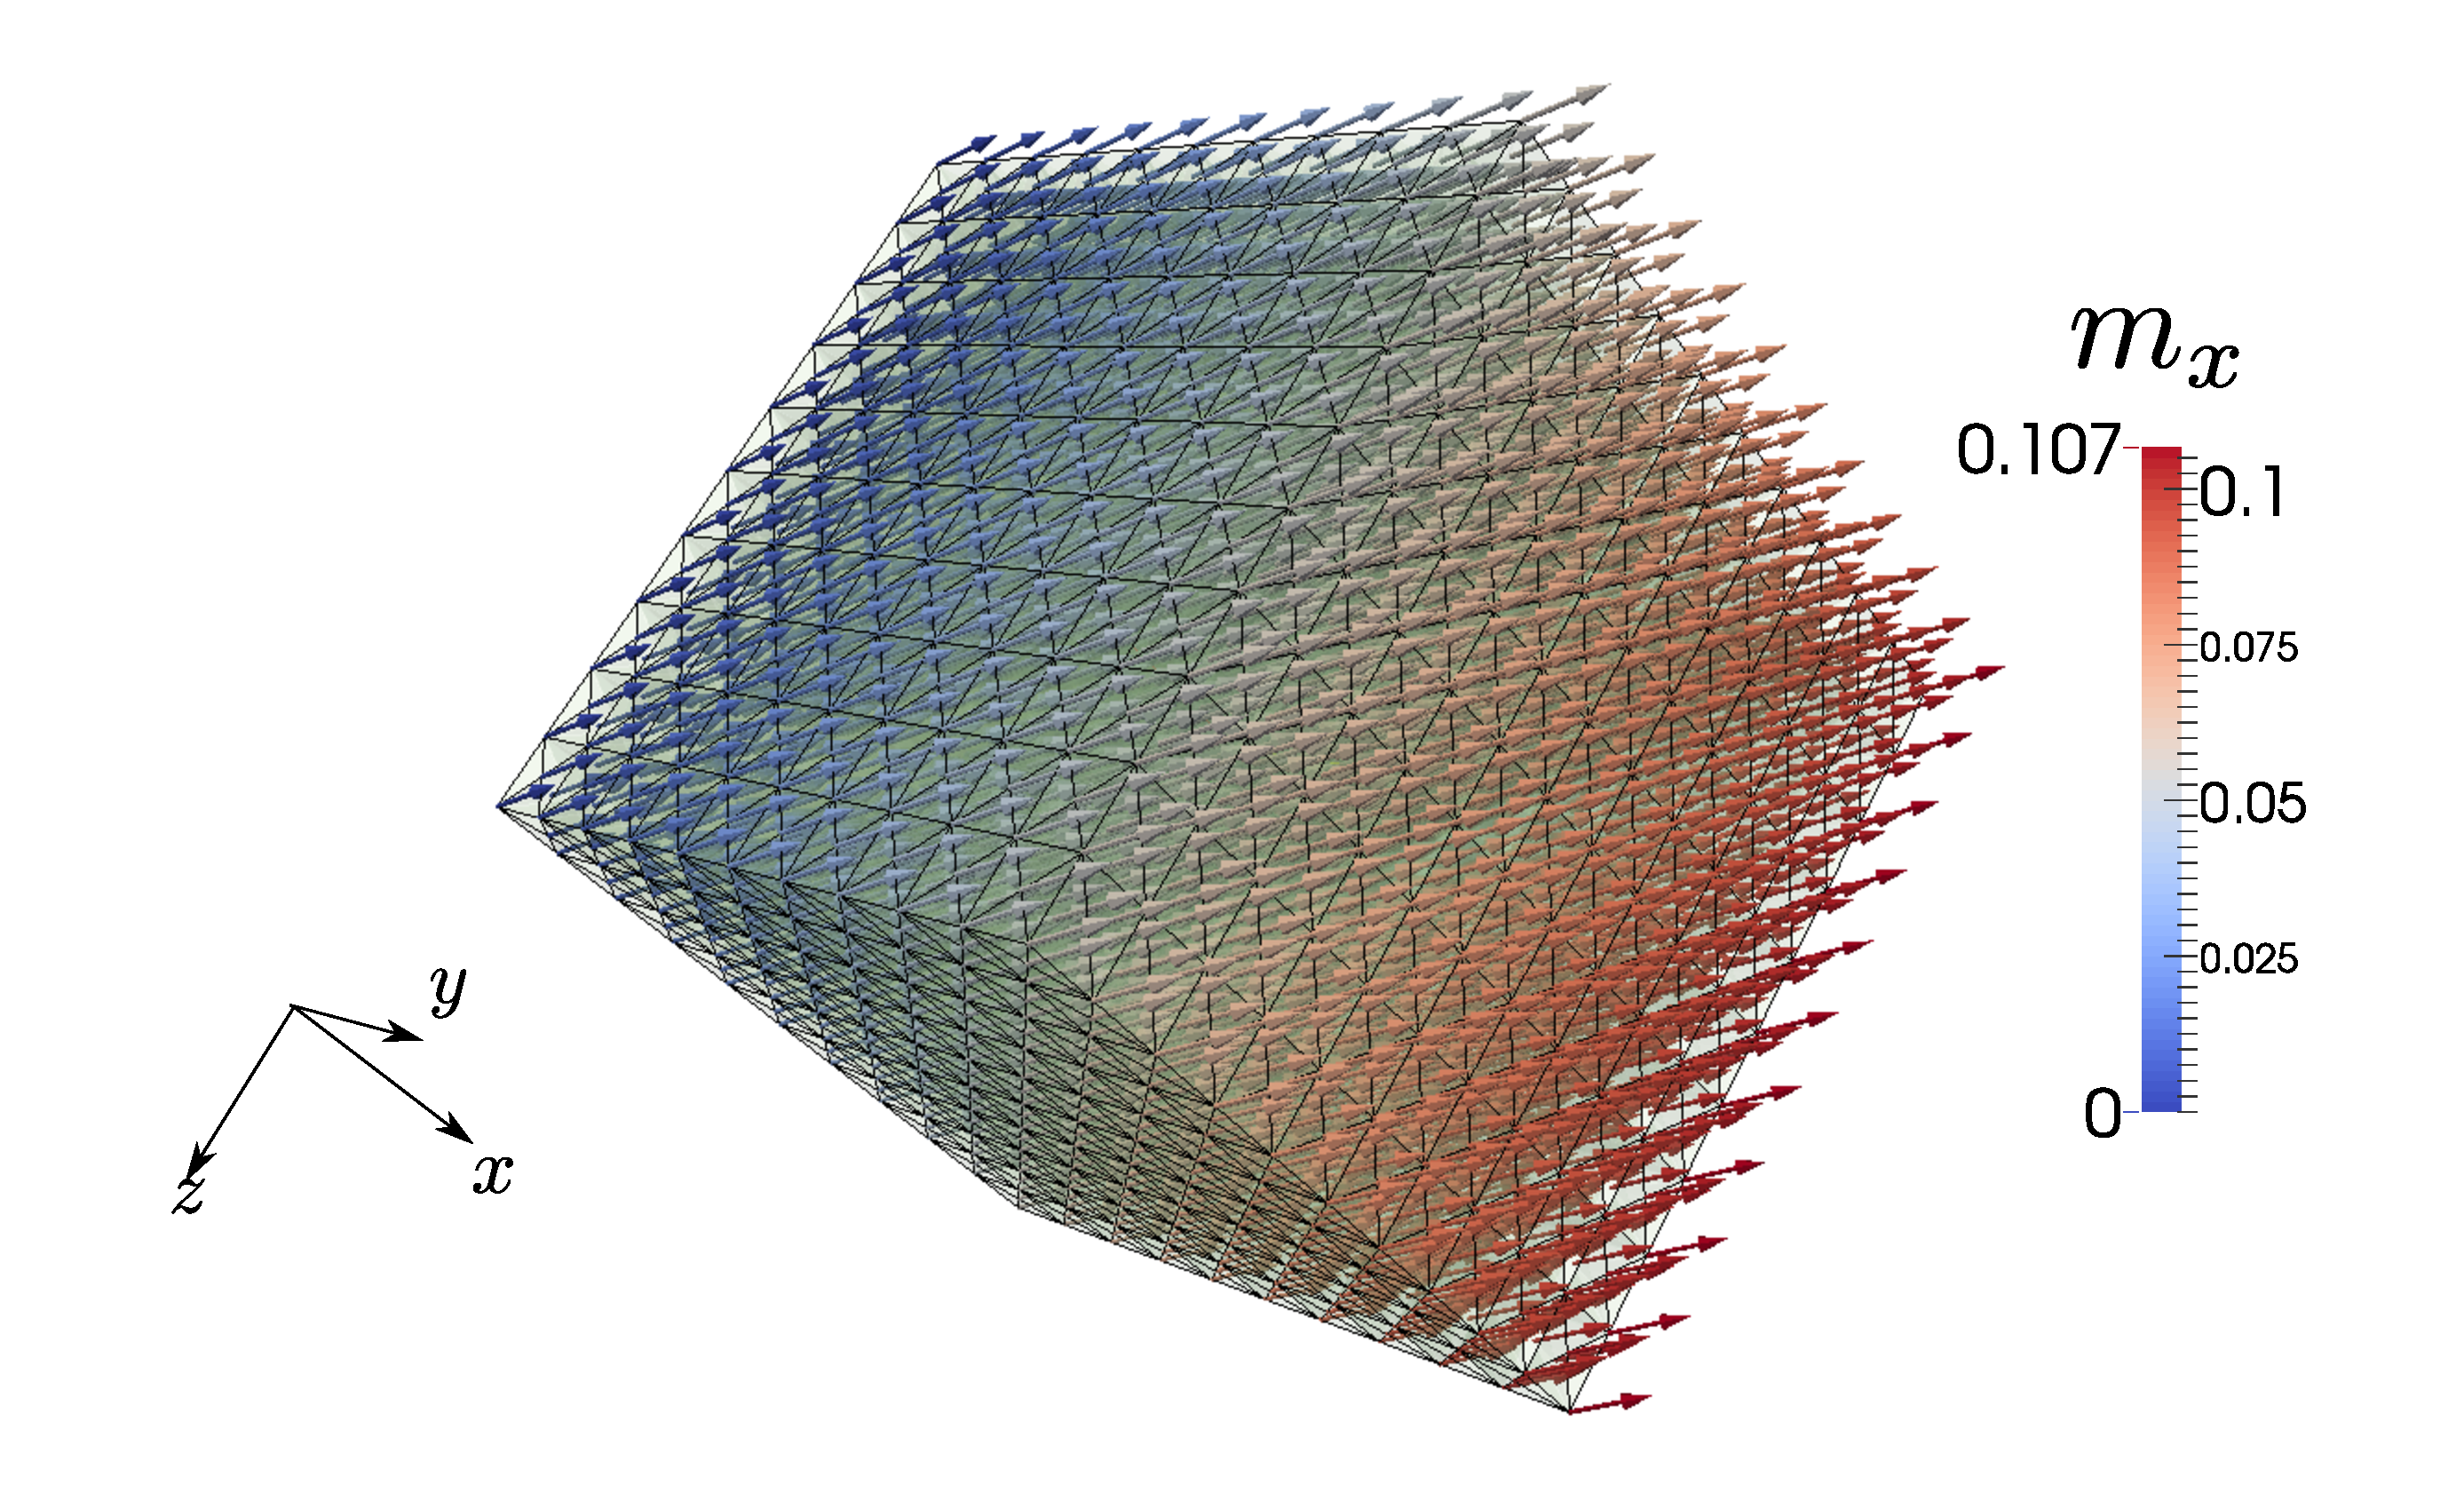
\includegraphics[width=0.8\textwidth]{images/itsacube}
  \caption{The test problem used for the linear solvers in the state at time $t=0$.
    The arrows represent the magnetisation direction at each node of the finite element mesh.
    Colour represents the magnitude of $m_x$.
    The semi-transparent pale green grid shows the finite element mesh.
  }
  \label{fig:cube-initial-condition}
\end{figure}


We use a range of damping and anisotropy parameters: $\dampc = 0, 0.01, 1$, $\kone = 0, 0.1$.
 % I should really have done $L=1,10,100$ (equivalent to varying exchange coeff), do it if there's time.
We use zero applied field to avoid inducing accidental symmetries.

\subsection{Implementation details}

Time steps of sizes $\dtn = 0.01, 0.1, 0.5, 1.0$ are chosen, and meshes with $\Nn= 71, 791, 5631, 42461$ nodes (note that the number of rows/columns in the Jacobian is roughly 5 times the number of nodes).
We use both the nodal quadrature discussed in \cref{sec:local-nodal-integr} and a standard Gaussian quadrature.
Since the only effect of changing the time integration methods on the linear systems is a small change to the constant in the time derivative terms we only run experiments using IMR.

The solvers are run both with and without the use of a hierarchical matrix representation for the dense $\Gm$ block.
We use the \hlib library \cite{hlib-website} with patches from \nmag \cite{nmag-website} allowing a collocation BEM approach.
For compatibility with this library we use a tetrahedral mesh.
We use the HCA II algorithm with parameters based on those used by Knittel \cite{Knittel2011}:
$\epsilon_{ACA} = 10^{-5}$,
minimum leaf matrix size $n_{\text{min}}= 30$,
admissibility criterion $\eta = 0.25$,
polynomial interpolation order $p=4$, and
numerical quadrature order $q=3$.
We also use adaptive recompression with $\epsilon = 10^{-3}$.

The CG and GMRES solvers used are \oomph's built-in implementations with relative convergence tolerances of $10^{-8}$.
GMRES with no restarts and left preconditioning is used for to ensure reliable convergence and reliable residual norms.
LU decomposition is implemented using the \superlu package \cite{superlu}.
The AMG implementation used as a preconditioner for Poisson matrices/blocks is \hypre's BoomerAMG \cite{hypre}.
One V(1,1) cycle with Gauss-Seidel smoothing, CLJP coarsening and a connection strength threshold of $0.7$ is used.
The ILU preconditioner used for LLG matrices/blocks is \hypre's Euclid with one level of fill in and no drop tolerance (ILU without fill-in was also tried but was extremely ineffective).


All experiments are run on a single core (\ie no parallelism is used) of a desktop computer with an Intel Core i7-3820 processor running at 3.6GHz and 16GB of RAM.


\subsection{Results}

Before presenting the results we note that, unless otherwise specified, all figures in this section show data points for all values of $\dtn$, $N$, $\dampc$ and $\kone$; both the nodal and Gaussian quadrature schemes; and both the dense and hierarchical $\Gm$ block formats.
However, where there appear to be no interesting differences caused by a parameter we plot data points for all values of that parameter using the same symbol and colour.
Also we note that occasionally data points overlap, giving the appearance of fewer points.

\Cref{fig:its-ilu-decoupled} shows the mean (over the linear solves required within a single Newton solve) number of GMRES iterations required to solve the LLG-only system, \cref{eq:llg-jacobian}, using ILU(1) preconditioning (\ie with magnetostatics handled by the semi-implicit approach).
As is expected for a general-purpose preconditioner it is effective for small matrix sizes, but becomes less effective for large problems and as the time step size increases.
% In fact for the largest $\Nn$ with the largest time steps ($\dtn = 1.0$) the solver does not converge with 400 iterations for some parameters.
The parameters $\dampc$ and $\kone$, along with the BEM block format and quadrature type do not appear to have a major impact on the effectiveness of the ILU(1) preconditioner in this example.
The mean preconditioner setup times this preconditioner are shown in \cref{fig:times-ilu-decoupled}.
As with the iteration counts, the setup times become significantly larger as $\Nn$ grows.

\newcommand{\manydatapointsTimeStepLegend}{Data points for all values of $\dampc$ and $\kone$; both types of quadrature; and both formats of the BEM block are shown but are not distinguished.}
\newcommand{\manydatapointsPrecLegend}{Data points for all values of $\dampc$, $\kone$, and for both formats of the BEM block are shown but are not distinguished.}

\newcommand{\newtonmean}{Mean (over a single Newton solve) of the}

\begin{figure}
  \centering
  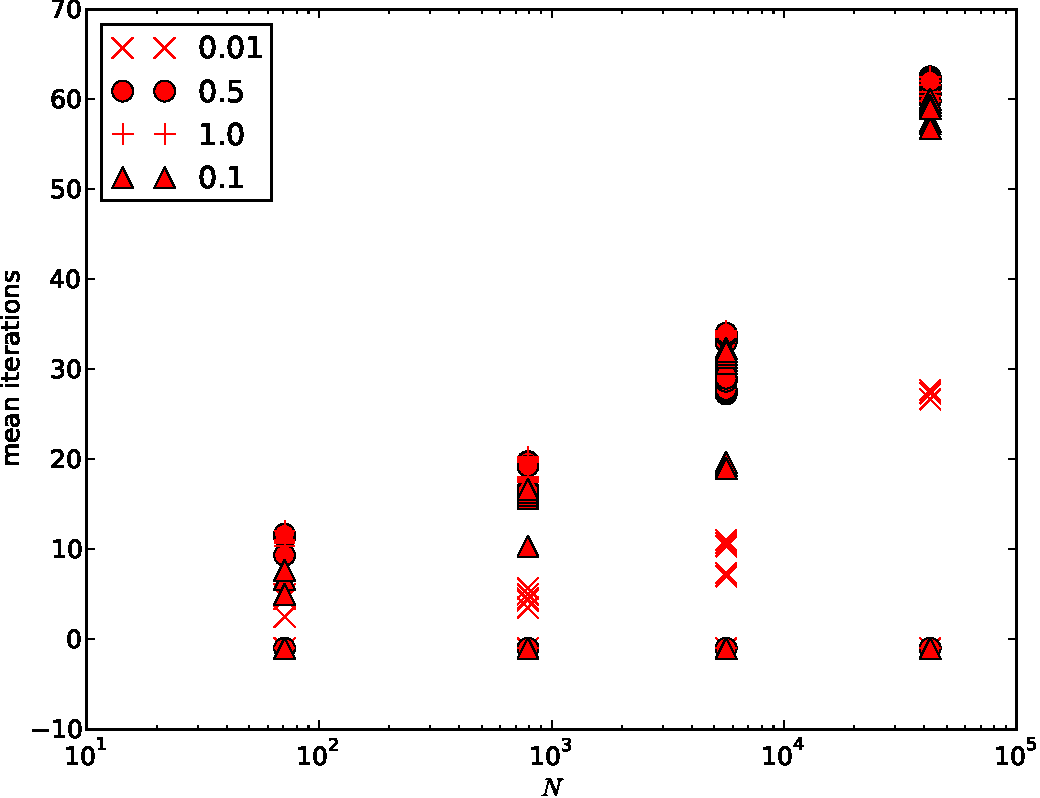
\includegraphics[width=0.8\textwidth]{plots/linear_solvers/ilu-1decoupleddummy-meanofnsolveritersvsinitialnnode.pdf}
  \caption{
    \newtonmean{}
    GMRES iterations to converge against problem size for the decoupled LLG preconditioned by ILU(1).
    The legend indicates the time step size.
    \manydatapointsTimeStepLegend{}
  }
  \label{fig:its-ilu-decoupled}
\end{figure}

\begin{figure}
  \centering
  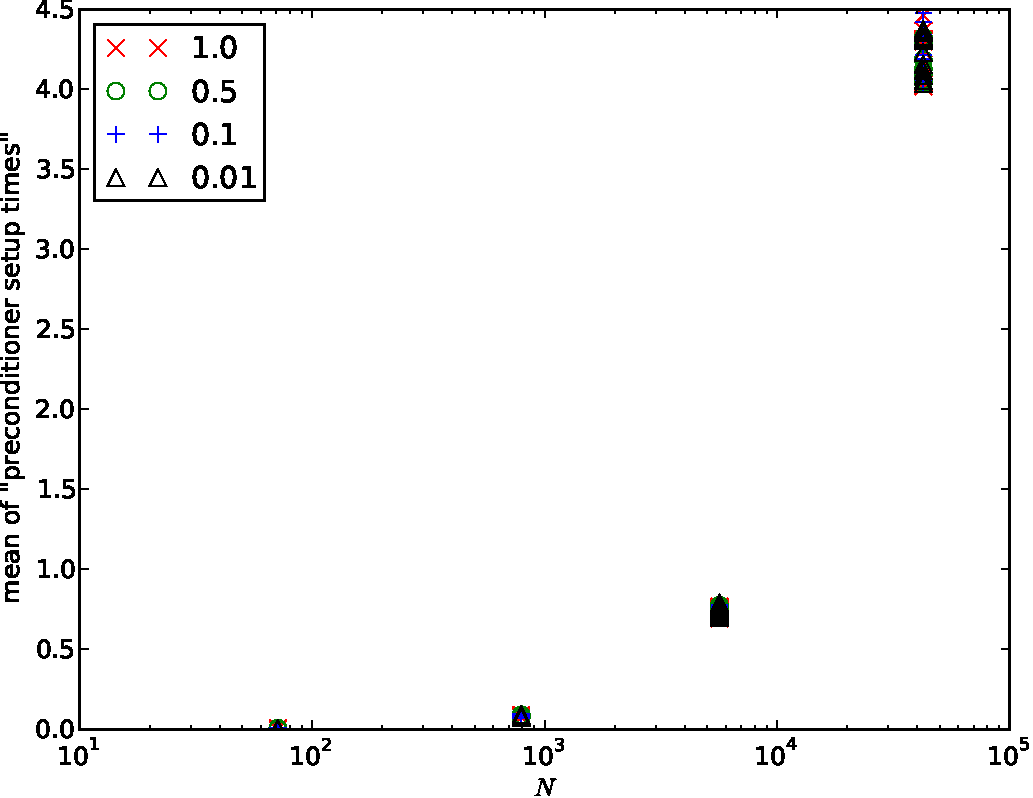
\includegraphics[width=0.8\textwidth]{plots/linear_solvers/ilu-1decoupleddummy-meanofpreconditionersetuptimesvsinitialnnode.pdf}
  \caption{
    \newtonmean{}
    time in seconds to set up an ILU(1) preconditioner against problem size for the decoupled LLG block.
    The legend indicates the time step size.
    \manydatapointsTimeStepLegend{}
  }
  \label{fig:times-ilu-decoupled}
\end{figure}


Next we consider the monolithic system \cref{eq:16} solved using preconditioner $\preca$, recall that this uses a direct solve of the sparse part of the Jacobian.
The iteration counts are shown in \cref{fig:its-p1-exact}.
Note that they are roughly independent of the number of nodes and vary only slightly with time step and the various other parameters.
However the preconditioner setup times, shown in \cref{fig:times-p1-exact}, rapidly increase with increasing matrix size as would be expected from a direct solve.
Also, due to the direct solve, the memory usage of this preconditioner is large.
Note that some data for the largest $\Nn$ are missing, this is because the memory required was more than the 16GB available.

\begin{figure}
  \centering
  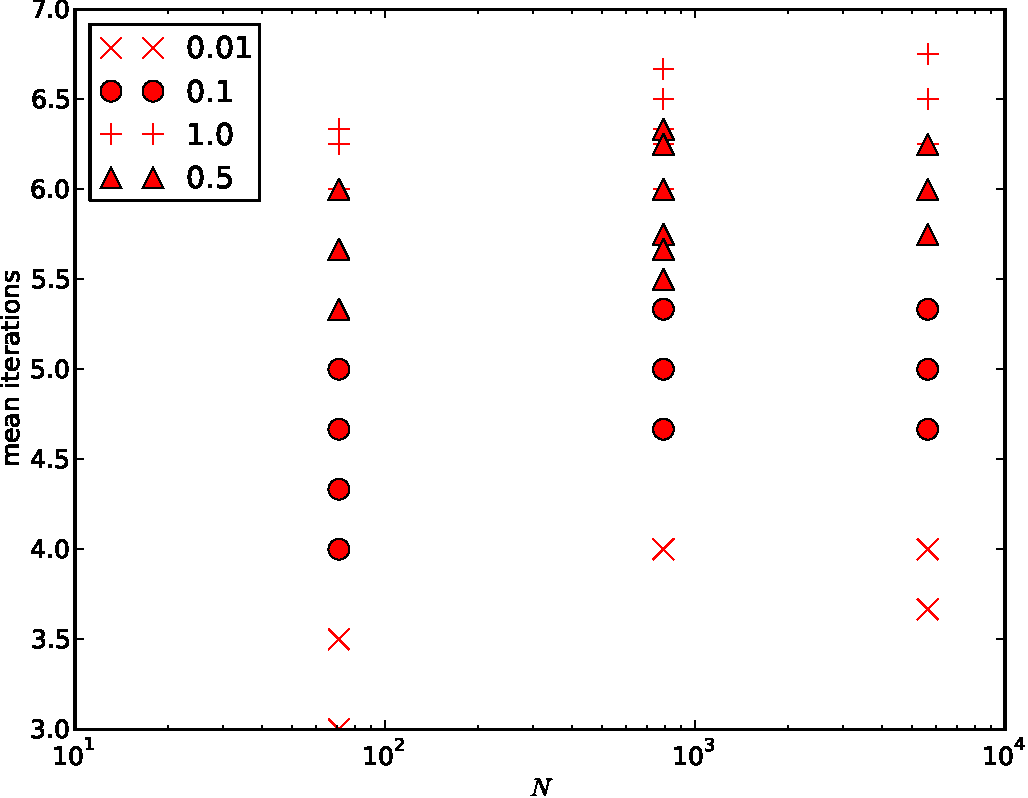
\includegraphics[width=0.8\textwidth]{plots/linear_solvers/som-main-exactimplicitdummy-meanofnsolveritersvsinitialnnode.pdf}
  \caption{
    \newtonmean{}
GMRES iterations to converge against problem size for the monolithic system preconditioned by $\preca$ (inverted by LU decomposition).
    The legend indicates the time step size.
    \manydatapointsTimeStepLegend{}
Some data points for the largest $\Nn$ are missing due the LU factors requiring more than 16GB of memory.
}
  \label{fig:its-p1-exact}
\end{figure}


\begin{figure}
  \centering
  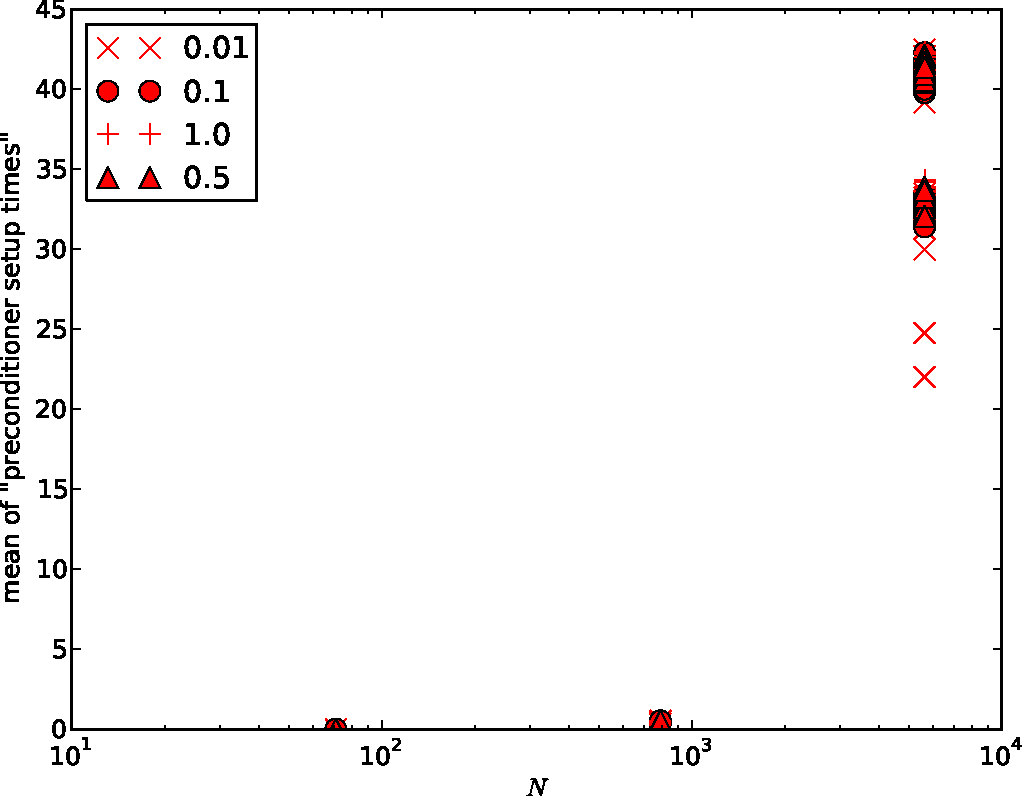
\includegraphics[width=0.8\textwidth]{plots/linear_solvers/som-main-exactimplicitdummy-meanofpreconditionersetuptimesvsinitialnnode.pdf}
  \caption{
    \newtonmean{}
    time in seconds to set up $\preca$ (inverted by LU decomposition) against problem size for the monolithic system.
    The legend indicates the time step size.
    \manydatapointsTimeStepLegend{}
    Some data points for the largest $\Nn$ are missing due the LU factors requiring more than 16GB of memory.
}
  \label{fig:times-p1-exact}
\end{figure}


Now we consider the partially-inexact preconditioners $\parinexact{\precb}$ and $\parinexact{\precc}$, which were designed to reduce the setup time and memory issues of $\preca$ by inverting part of the preconditioner approximately using iterative methods.
The iteration counts are shown in \cref{fig:its-p23-exact}, we see that for both preconditioners the number of iterations increases only slightly as the number of nodes increases and that the various other parameters have little impact on their effectiveness.
Also note that the iteration counts are not much larger than those of $\preca$.
The preconditioner setup times are shown in \cref{fig:times-p23-exact}.
They are significantly smaller than those in \cref{fig:times-p1-exact} but still grow unacceptably large due to the direct solve of the $\Fm$ block.
Interestingly the use of nodal integration decreases the time required for the setup of the preconditioner.
This is likely due to the ``mass-lumping'' effect discussed in \cref{sec:local-nodal-integr}.
However it does not decrease the time sufficiently for the preconditioner to be viable for practical usage on problems with number of nodes $\Nn \gtrsim 10^4$.
Also of note is that, unlike $\preca$, the required LU decomposition fits within the 16GB of available memory for all parameters.

\begin{figure}
  \centering
  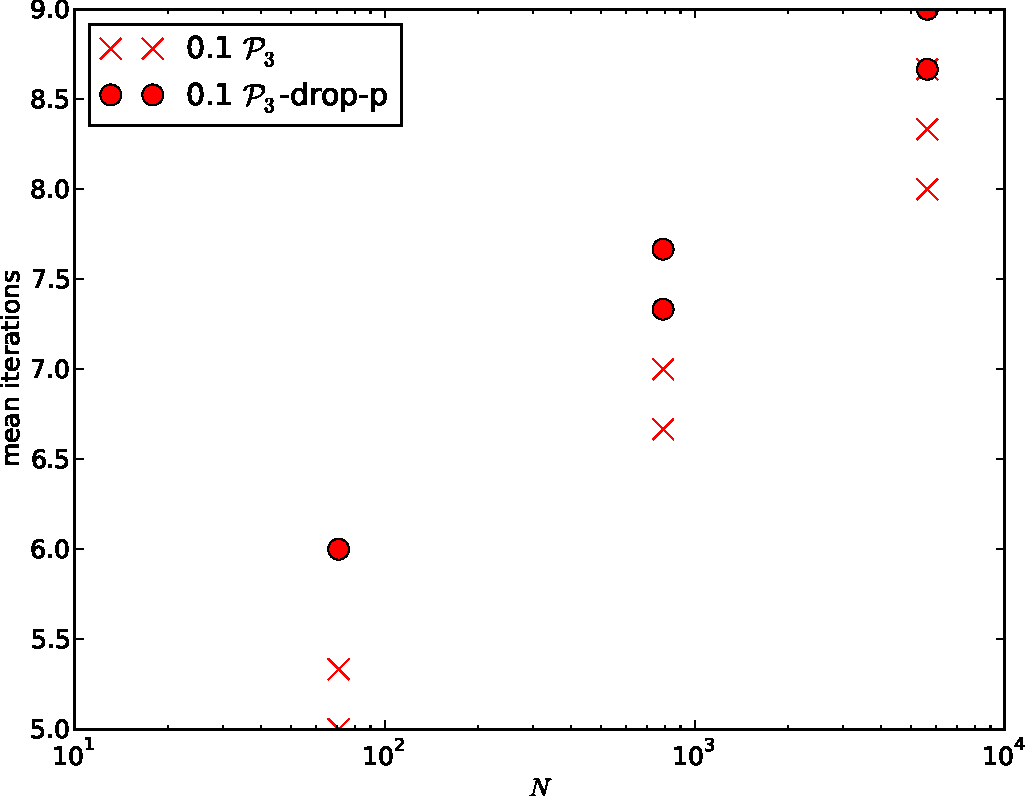
\includegraphics[width=0.8\textwidth]{plots/linear_solvers_p2p3/implicitexact-meanofnsolveritersvsinitialnnode.pdf}
  \caption{
    \newtonmean{}
    GMRES iterations to converge against problem size for the monolithic system using the partially-inexact preconditioners $\parinexact{\precb}$, $\parinexact{\precc}$ with $\dtn=0.1$.
The legend indicates the preconditioner and quadrature scheme used.
\manydatapointsPrecLegend{}
}
  \label{fig:its-p23-exact}
\end{figure}

\begin{figure}
  \centering
  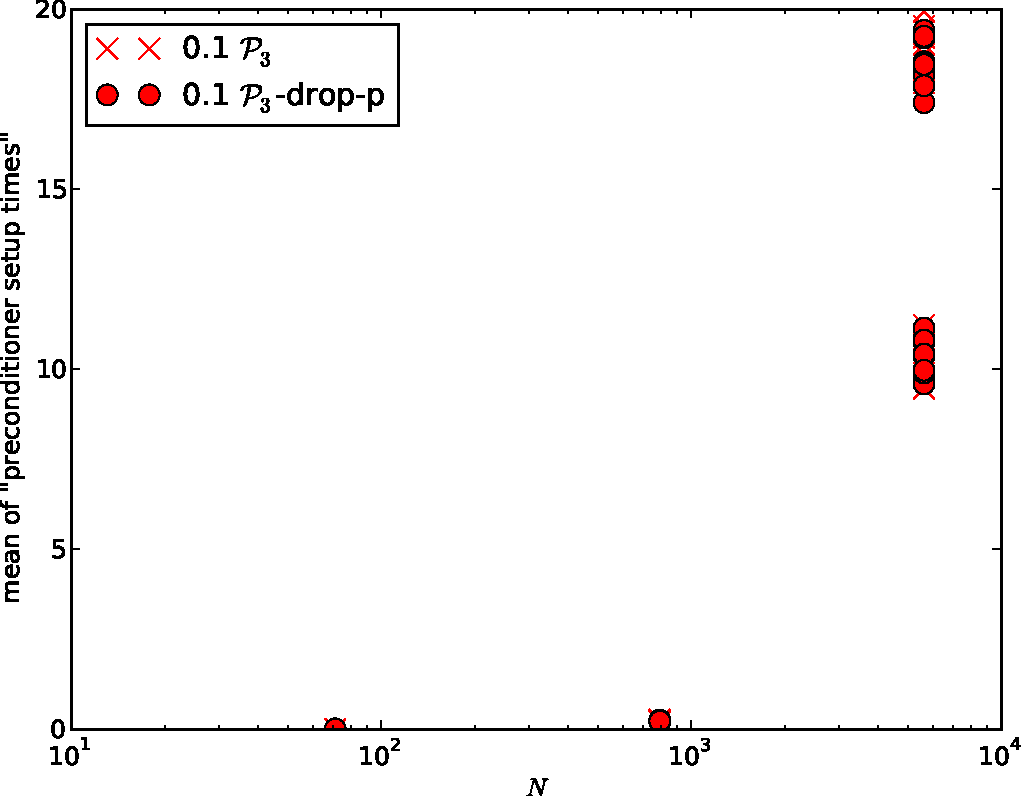
\includegraphics[width=0.8\textwidth]{plots/linear_solvers_p2p3/implicitexact-meanofpreconditionersetuptimesvsinitialnnode.pdf}
  \caption{
    \newtonmean{}
    time in seconds to set up the partially-inexact preconditioners $\parinexact{\precb}$, $\parinexact{\precc}$ against problem size for the monolithic system with $\dtn=0.1$.
    The legend indicates the preconditioner and quadrature scheme used.
    \manydatapointsPrecLegend{}
}
  \label{fig:times-p23-exact}
\end{figure}


Finally we show iteration counts for the fully-inexact preconditioners $\inexact{\precb}$ and $\inexact{\precc}$ where the $\Fm$ block is approximated using ILU(1).
We cannot expect $\Nn$-independent results here, since even the simpler case of the solution of the $\Fm$ block alone with GMRES preconditioned by ILU(1) does not display such behaviour.
The iteration counts shown in \cref{fig:its-p23-ilu1}, are as expected: low at first but ineffective for large number of nodes $\Nn$.
In particular, for the largest number of nodes GMRES did not converge within 400 iterations for any of the parameter sets.
Also of note is the much larger variation of the iteration counts with the problem parameters even for the same problem size.
However the preconditioner setup times, as shown in \cref{fig:times-p23-ilu1} are much better than when using the LU decomposition of the $\Fm$ block.

% could try to find/show parameter dependency: some iteration counts are ok!

\begin{figure}
  \centering
  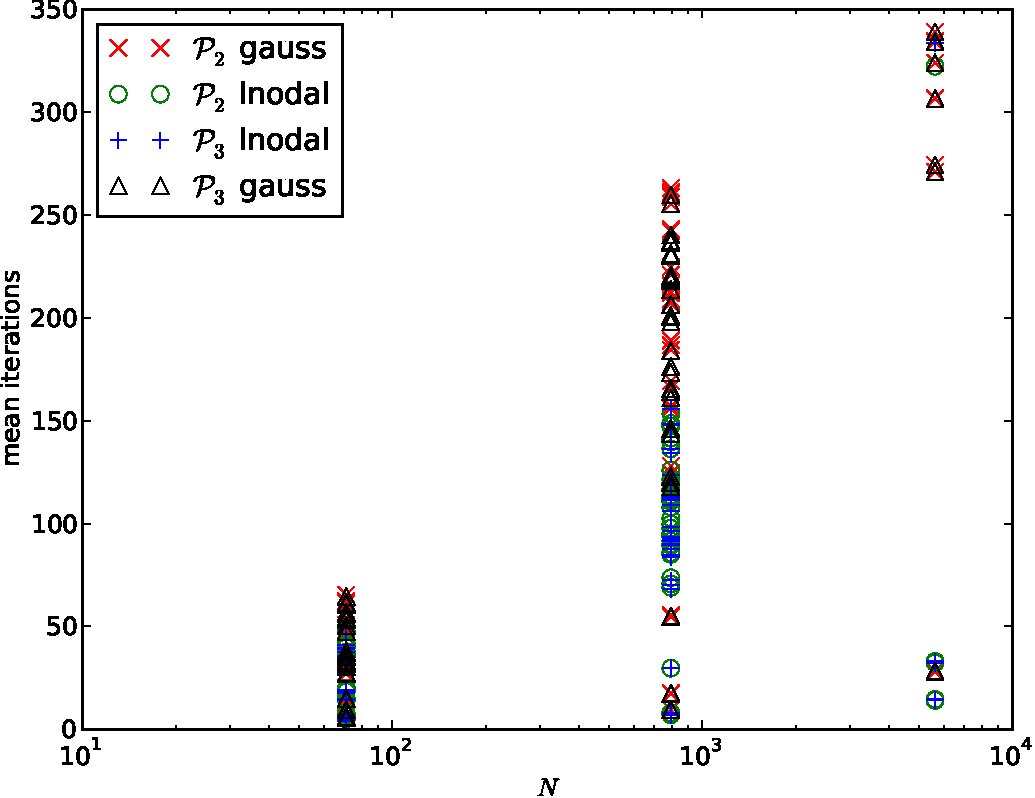
\includegraphics[width=0.8\textwidth]{plots/linear_solvers_p2p3/implicitilu-1-meanofnsolveritersvsinitialnnode.pdf}
  \caption{
    \newtonmean{}
    GMRES iterations to converge against problem size for the monolithic system using the inexact preconditioners $\inexact{\precb}$, $\inexact{\precc}$ with $\dtn=0.1$.
    The legend indicates the preconditioner and quadrature scheme used.
    \manydatapointsPrecLegend{}
    Some data points are missing for the largest $\Nn$ due to a lack of convergence.
  }
  \label{fig:its-p23-ilu1}
\end{figure}

\begin{figure}
  \centering
  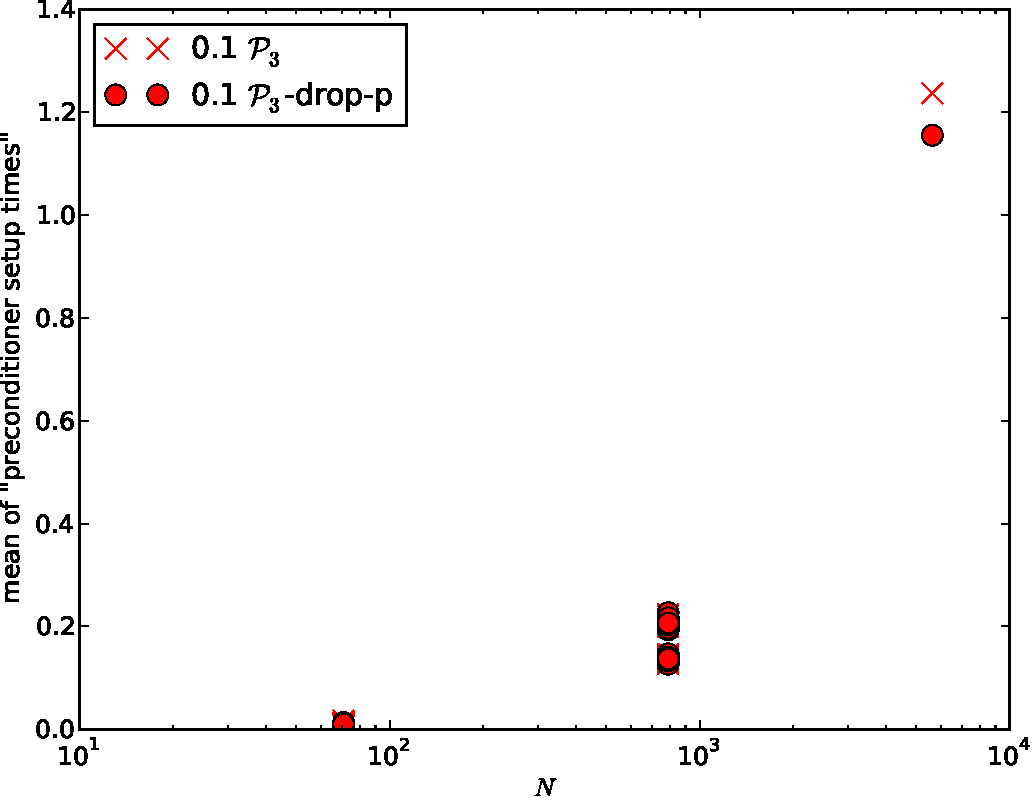
\includegraphics[width=0.8\textwidth]{plots/linear_solvers_p2p3/implicitilu-1-meanofpreconditionersetuptimesvsinitialnnode.pdf}
  \caption{
    \newtonmean{}
    time in seconds to set up the inexact preconditioners $\inexact{\precb}$, $\inexact{\precc}$ against problem size for the monolithic system with $\dtn=0.1$.
    The legend indicates the preconditioner and quadrature scheme used.
    \manydatapointsPrecLegend{}
    Some data points are missing for the largest $\Nn$ due to a lack of convergence.
  }
  \label{fig:times-p23-ilu1}
\end{figure}

% Effect of HLib? If time do this later


% if I get inner iteration preconditioner working then compare the total solve time for the semi-implicit method (with GMRES and ILU-1 preconditioning) and fully implicit method (with $\precb$, ILU-1 for the $\Fm$ block or maybe using BiCGstab for F?), both using HLib.
% No chance of this now...

\section{Outlook}
\label{sec:furth-optim-opport}

We now compare the \emph{expected} performance of the monolithic and semi-implicit approaches with the assumption that a ``sufficiently good'' preconditioner for the $\Fm$ block can be found and discuss further improvements that could be made.

First we examine the relative cost of the assembly of the Jacobian matrices and Newton residuals.
As mentioned above the Jacobian matrices corresponding to linear equations are only dependent  on the geometry and so do not need to be recomputed at each Newton step.
So the Poisson Jacobians and the LLG-Poisson coupling blocks ($\Qm$ and $\Pm$ from \cref{eq:16}) do not need to be recomputed.
This means that for both methods only assembly of the $\Fm$ block is required, and the computation time is identical.

As an aside: the mass matrix blocks on the diagonal of $\Fm$ ($\Mm$ of \cref{eq:llg-jacobian}) are also linear.
Additionally the skew symmetric structure of \cref{eq:llg-jacobian} can be exploited so that the calculation of $\Km_x$ is reused for $-\Km_x$, and similarly for $\Km_y$ and $\Km_z$.
Applying these additional optimisations reduces the Jacobian calculations to the assembly of three $\Nn \times \Nn$ Jacobian blocks and the magnetocrystalline anisotropy block (which will typically be either a single $\Nn \times \Nn$ block or empty, see \cref{sec:llg-jacobian}).

In practice the Newton residual assembly time is extremely small compared to the solve and Jacobian assembly times ($\sim 99 \%$ of the time in the non-linear solver is spent in the Jacobian assembly and linear solves).
So the computation time difference due to assembling additional $\phim$ and $\phione$ residual components in Newton steps after the first can be ignored.

We now examine the cost per Krylov iteration (or per set of Krylov iterations for the decoupled case).
The monolithic approach has more non-zeros in the Jacobian (the P, Q, G blocks), giving approximately $4 \Nn$ extra matrix elements, compared to a base of $11 \Nn$, hence approximately one third as much time again is taken for each Krylov step.
Also our fully coupled method uses GMRES for all blocks rather than GMRES for $\Fm$ and CG for the two Poisson blocks.
Since GMRES requires a more computationally expensive orthogonalisation process than CG this will increase the cost of the monolithic approach as compared to the semi-implicit approach.
This increase could possibly be reduced by using BiCGStab or a restarted GMRES method instead of GMRES.
Finally it is likely that the monolithic method will require more Krylov iterations to converge, but with a good preconditioner for the $\Fm$ block this difference should be fairly small.

Based on all these factors we speculate that, with an effective preconditioner for the LLG block, the computational time for a monolithic time step should be within a factor of 2 of the time for a semi-implicit step.


\section{Conclusions and future work}

Monolithic (fully implicit) solvers are required for the energy property of IMR, as well as for other properties of implicit time integration schemes including stability and properties important in stochastic problems.
We have demonstrated that a monolithic LLG-magnetostatics solver using GMRES with an effective preconditioner can result in a reasonable computational cost per linear solve.
The partially-inexact preconditioners $\parinexact{\precb}$ and $\parinexact{\precc}$ are able to reduce the iteration count of GMRES extremely effectively and almost independently of the number of nodes, but the set up cost is high for large matrices.
However the fully-inexact equivalents, $\inexact{\precb}$ and  $\inexact{\preca}$, which use ILU(1) to approximate the LLG block are ineffective for more than a few thousand nodes (\ie matrices of size $\sim 10,000$).
Hence cheap, effective and mesh independent preconditioning methods for the LLG block, $\Fm$, are still needed for the monolithic block-preconditioned method discussed here to be effective on general large problems.

We have also demonstrated solvers for a decoupled LLG block solve, for medium numbers of nodes it appears that ILU(1) is a good preconditioner for this case.
However, the time integration properties of the semi-implicit scheme using this solve have yet to be seen.


For granular or bit patterned media a domain-decomposition preconditioner exploiting the low/zero exchange coupling between grains/islands could make for a simple but effective domain decomposition preconditioner.
For example, such a preconditioner could be implemented by performing an independent direct solve on the matrix block associated with each grain/island and using this diagonal block solution as the preconditioner.
Since the number of nodes in a single grain/island is small and fixed this would remain effective even for very large numbers of grains/islands.

Reordering of the degrees of freedom, scaling, drop tolerance, fill-in level in the ILU preconditioner could be experimented with further to allow the solution of larger systems or alternative parameters \cite[287]{Saad2000}.
However, ILU preconditioning is unlikely to ever give $\Nn$-independent or parameter-independent results, so it may not be the best path towards more general efficient preconditioners.




%%% Local Variables:
%%% mode: latex
%%% TeX-master: "main"
%%% End:


% In the plots:
% consistent colours?
% max(m-1) -> m-1

% Check with Matthias:
% * c.f. = compare with (like ie, eg) is that ok to use?


% Check with Milan:
% why is TR dt growing slower in stiff example? ringing? citation?


% Fixup ebdf3 code and include in oomph-lib

\chapter{An adaptive implicit midpoint rule scheme}
\chaptermark{Adaptive IMR}
\label{sec:adaptive-imr}


The implicit midpoint rule (IMR) is a well known integration scheme for initial value ordinary differential equations (ODEs) with favourable stability and accuracy properties (see \cref{sec:time-discretisation} or \cite[204]{HairerNorsettWanner}).
It also has beneficial ``geometric integration'' properties when applied to the time integration of the Landau-Lifshitz-Gilbert equation (discussed in \cref{sec:ensuring-constant-mv,sec:energy-cons}).
However it is a non-trivial task to create an efficient adaptive time step selection algorithm for the IMR using typical approaches.

In \thisref{sec:adaptive-imr} we describe a novel adaptive IMR algorithm based on efficient estimates of the local truncation error by an explicit step.
We then demonstrate the effectiveness of this algorithm on a number of ODE test problems in \cref{sec:aimr-testing} and an ODE form of the LLG in \cref{sec:imr-ode-llg-numer-exper}.
Experiments on a full PDE LLG problem are performed in \cref{cha:numer-experiments}.


\section{The implicit midpoint rule with fixed step size}
\label{sec:fixed-step-implicit}

Let $\yv(t)$ be a vector function and denote an approximation to $\yv(t)$ at $t = t_n$ by $\yv_n$.
Let $\dtn = t_{n+1} - t_n$ be the $n$th time step (or just ``step'').
Then, given a system of ordinary differential equations (ODEs) of the form
\begin{equation}
  \yv'(t) = \ffv{t, \yv(t)},
  \label{eq:43}
\end{equation}
the implicit midpoint rule (IMR) is
\begin{equation}
    \yv_{n+1} = \yv_n + \dtn \ffv{\frac{t_{n+1} + t_n}{2}, \frac{\yv_n + \yv_{n+1}}{2}}.
    \label{eq:67}
\end{equation}

We introduce shorthand notation for the midpoint values of $t$ and $\yv$:
\begin{equation}
  \begin{aligned}
    \thf & = \frac{t_{n+1} + t_n}{2} \quad \bigb{= t_n + \frac{\dtn}{2}}, \\
    \yvm &= \frac{\yv_{n+1} + \yv_n}{2}.
  \end{aligned}
\end{equation}
In this notation the IMR is
\begin{equation}
  \yv_{n+1} = \yv_n + \dtn \ffv{\thf, \yvm}.
  \label{eq:basic-midpoint}
\end{equation}

The IMR can also be written in the standard form for implicit Runge-Kutta methods as
\begin{equation}
  \begin{aligned}
    k_1 &= \ffv{t_n + \frac{1}{2} \dtn, \yv_n + \frac{1}{2} k_1}, \\
    \yv_{n+1} &= \yv_n + 1 \cdot \dtn k_1,
  \end{aligned}
\end{equation}
which is equivalent to the Butcher tableau \cite[135]{HairerNorsettWanner} shown in \cref{tab:butcher-imr}.

\begin{table}
  \begin{equation*}
    \begin{array}{c|c}
      \frac{1}{2}  &     \frac{1}{2}  \\
      \hline
                   & 1 \\
    \end{array}
  \end{equation*}
  \caption{The Butcher tableau for the implicit midpoint rule.}
  \label{tab:butcher-imr}
\end{table}

Note that, unlike for multistep methods, \cref{eq:basic-midpoint} is valid for both constant and variable step sizes because there is no dependence on previous steps.


\section{Adaptive implicit midpoint rule}
\label{sec:adapt-impl-midp}

Adaptive time step selection algorithms are typically based on approximating the local truncation error (LTE), the error due to a single step of the integration scheme (see \cref{sec:deriv-local-trunc}).
These estimates can be used to select appropriate time steps such that the LTE remains close to a specified value.
In \thisref{sec:adapt-impl-midp} we first discuss why the standard approaches used to estimate the LTE fail for the IMR, and the approach that we will use.
We next derive the formulae required and discuss how a complete adaptive time step selection algorithm can be implemented using the LTE estimates.


\subsection{Construction of an LTE estimate}

Due to the complexity of the LTE of the implicit midpoint rule (as compared with those of TR or BDF2) there are difficulties with the Milne-device approach described in \cref{sec:adaptivity}.
In particular, the LTE of IMR has a term involving the error due to the approximation $\yv(\thf) \sim \yvm$ (term II of \cref{eq:trunc-mid}).
In order to perform the algebraic rearrangements to obtain the LTE using a Milne-device-like approach we would need this term to appear in the LTE of the predictor.
However the term can only appear in the LTE expression for a time integrator which uses the midpoint approximation for $\yv$.
It turns out that the only such second order time integrator is IMR itself.
So other techniques would be needed to approximate this error term in the context of a Milne-device-like method.

An alternative approach, commonly used in Runge-Kutta time integrators, is to repeat the calculation using a higher order method and compare the two answers to directly obtain an LTE estimate \cite[165]{HairerWanner}.
However evaluations of the derivative function ($\fv$ in \cref{eq:43}) are expensive, and the calculation of a single step of a high order Runge-Kutta method requires a number of such evaluations.
Hence such approaches usually rely on pairs of Runge-Kutta methods which share most of their derivative evaluation points but have different orders of accuracy.
These are known as embedded Runge-Kutta methods, a widely used example is the Dormand–Prince pair (order 4/5) used in MATLAB's \texttt{ode45} function \cite{matlab-ode45}.

Unfortunately there is no third order method which requires only $\ffv{\thf, \yvm}$ and a single other function evaluation.\footnote{IMR's single function evaluation is positioned such that the second order error terms cancel. Adding one additional evaluation cannot retain the symmetry causing this cancellation and so does not increase the order, at least two additional evaluations are needed.}
To get around this problem we instead use an explicit multistep method: the explicit version of the third order backwards difference method (eBDF3).
This method requires three history values but only a single explicit function evaluation in order to compute a 3rd-order-accurate approximation to $\yv(t_{n+1})$.
Since only one function evaluation is required the computational cost is equivalent to an embedded Runge-Kutta method.
With this approach our estimate for the local truncation error is simply
\begin{equation}
  \label{eq:aimr-lte-est}
  \lte = \yv_{n+1}^{\ebdf} - \yv_{n+1}^\imr + \order{\dtn^4}.
\end{equation}
The eBDF3 method is not widely used because it does not have the basic property essential for time integration \cite[365]{HairerNorsettWanner}:
\begin{equation}
  \lim_{\dtn \rightarrow 0} \bigb{ \max_n \norm{\yv_{n} - \yv(t_n)}} = 0,
  \label{eq:104}
\end{equation}
which is known variously as ``stability'' \cite[378]{HairerNorsettWanner} or ``convergence'' \cite[6]{Iserles2009}.
However, for our usage the IMR history values are used as input for a \emph{single} step of eBDF3, hence the stability is irrelevant.\footnote{This could also be thought of as an extrapolation to the value of $\yv$ at $t_{n+1}$ using the previous IMR-generated values and a derivative.}
The variable time step version of eBDF3 does not appear in the literature, so we derive the method below in \cref{sec:variable-step-ebdf3} .

Alternatively a 3rd order Adams-Bashforth scheme (AB3) could be used, but this would require three previous derivative values instead of $y$ values making the initialisation of the scheme a little more complex and expensive.
Additionally, the calculation of coefficients for the variable step Adams-Bashforth schemes is more complex \cite[400]{HairerNorsettWanner}.
However, in contrast to eBDF3, AB3 has the basic property \cref{eq:104} which could simplify the process of testing an implementation.


\subsection{The variable step eBDF3 method}
\label{sec:variable-step-ebdf3}

The explicit BDF methods are explicit time integration methods derived using the same techniques as the widely used implicit BDF methods.
The idea is to write down a divided difference representation of an interpolating polynomial, $\pv(t)$, through $\yv_{n+1}$ and the appropriate history values of $\yv$ (simple backward differences can be used for constant time steps, hence the name).
The derivative of the polynomial is then set equal to the derivative function $\ffv{t, \yv}$ at one of the discrete time steps \cite[400]{HairerNorsettWanner}.
Setting $\pv'(t_{n+1}) = \ffv{t_{n+1}, \yv_{n+1}}$ gives the widely used implicit BDF methods.
If we instead set $\pv'(t_{n}) = \ffv{t_{n}, \yv_{n}}$ we obtain the explicit BDF methods \cite[364]{HairerNorsettWanner}.
We now derive the first three eBDF methods.
% The derivation of the implicit BDF methods is shown in \cref{cha:deriv-impl-backw} and may be useful for comparison.

For this purpose we define the Newton divided differences recursively by
\begin{equation}
  \label{eqn:divided-diff}
  \begin{aligned}
    \yv[t_{n+1}] &= \yv_{n+1}, \\
    \yv[t_{n+1}, t_n] &= \frac{\yv[t_{n+1}] - \yv[t_n]}{t_{n+1} - t_n}, \\
    \yv[t_{n+1}, t_n, t_{n-1}] &= \frac{\yv[t_{n+1}, t_n] - \yv[t_n, t_{n-1}]}{t_{n+1} - t_{n-1}}, \\
    \vdots
  \end{aligned}
\end{equation}
The $k$-th Lagrange interpolation polynomial \cite[124]{BurdenFaires}, \cite[400]{HairerNorsettWanner} can be expressed using these as
\begin{equation}
  \label{eqn:divided-diff-intp}
  \begin{aligned}
    \pv_k(t) &= \yv_{n+1} + \sum_{j=1}^k \yv[t_{n+1}, \ldots, t_{n+1-j}] \prod_{i=0}^{j-1} (t - t_{n+1-i}), \\
    &= \yv_{n+1} + \yv[t_{n+1}, t_n](t - t_{n+1}) + \yv[t_{n+1}, t_n, t_{n-1}](t - t_{n+1})(t - t_n) \\
    &\quad + \yv[t_{n+1}, t_n, t_{n-1}, t_{n-2}](t - t_{n+1})(t - t_n)(t - t_{n-1}) + \ldots \\
    &\quad + \yv[t_{n+1}, \ldots, t_{n+1-k}](t-t_{n+1})\cdots(t-t_{n-k}).
  \end{aligned}
\end{equation}
Differentiating \cref{eqn:divided-diff-intp} with respect to $t$, recalling that divided differences are constants and applying the chain rule to the derivative of the product term we obtain
\begin{equation}
  \begin{aligned}
    \pv_k'(t) &= \yv[t_{n+1}, t_n] + \yv[t_{n+1}, t_n, t_{n-1}]\bigb{(t - t_n) + (t - t_{n+1})} \\
    &\quad + \yv[t_{n+1}, t_n, t_{n-1}, t_{n-2}]\big( (t - t_n)(t - t_{n-1}) + (t - t_{n+1})(t - t_{n-1})\\
    &\qquad \qquad  + (t - t_{n+1})(t - t_n) \big) \\
    &\quad + \ldots \\
    &\quad + \yv[t_{n+1}, \ldots, t_{n+1-k}]\big( (t-t_{n})\cdots(t-t_{n-k}) \\
    &\qquad \qquad + \ldots + (t-t_{n+1})\cdots(t-t_{n-k+1}) \big), \\
    &= \sum_{j=1}^k \yv[t_{n+1}, \ldots, t_{n+1-j}] \sum_{l=0}^{j-1}
    \prod_{i=0, i \neq l}^{j-1} (t - t_{n+1-i}).
    \label{eq:59}
  \end{aligned}
\end{equation}
Setting $\ffv{t_n, \yv_n} = \pv_k'(t_n)$ results in
\begin{equation}
  \begin{aligned}
    \ffv{t_n, \yv_n} &= \sum_{j=1}^k \yv[t_{n+1}, \ldots, t_{n+1-j}] \sum_{l=0}^{j-1} \prod_{i=0, i \neq l}^{j-1} (t_n - t_{n+1-i}).
  \end{aligned}
\end{equation}
This can be greatly simplified by noticing that the product $ \prod_{i=0, i \neq l}^{j-1} (t_n - t_{n+1-i})$ is zero whenever it contains $i=1$, \ie whenever $j \geq 2$ and $l \neq 1$.
When $j=1$ the only non-zero terms in the sum of products are for $l=0$ and $i=0$, so we only need to consider the case of $l=1$.
This gives
\begin{equation}
  \begin{aligned}
    \ffv{t_n, \yv_n} &= \sum_{j=1}^k \yv[t_{n+1}, \ldots, t_{n+1-j}] \prod_{i=0, i \neq 1}^{j-1} (t_n - t_{n+1-i}), \\
    &= \yv[t_{n+1}, t_n] + \sum_{j=2}^k \yv[t_{n+1}, \ldots, t_{n+1-j}] \prod_{i=0, i \neq 1}^{j-1} (t_n - t_{n+1-i}), \\
    &= \yv[t_{n+1}, t_n] -\dtn \sum_{j=2}^k \yv[t_{n+1}, \ldots, t_{n+1-j}] \prod_{i=2}^{j-1} (t_n - t_{n+1-i}). \\
  \end{aligned}
  \label{eq:ebdf-general}
\end{equation}

For $k=1$ equation \cref{eq:ebdf-general} reduces to
\begin{equation}
  \begin{aligned}
    \fv(t_n, \yv_n) &= \yv[t_{n+1}, t_n] = \frac{\yv_{n+1} - \yv_n}{\dtn}, \\
    \yv_{n+1} &= \yv_n + \dtn f(t_n, \yv_n), \\
  \end{aligned}
\end{equation}
which is the forward Euler method.

For $k=2$ we have
\begin{equation}
  \begin{aligned}
    \fv(t_n, \yv_n) &= \yv[t_{n+1}, t_n] - \dtn \yv[t_{n+1}, t_n, t_{n-1}] , \\
    &=  \frac{\yv_{n+1} - \yv_n}{\dtn}
    - \frac{\dtn}{\dtn + \dtx{n-1}} \bigb{ \frac{\yv_{n+1} - \yv_n}{\dtn} - \frac{\yv_n - \yv_{n-1}}{\dtx{n-1}}}.
  \end{aligned}
\end{equation}
After some algebra this gives
\begin{equation}
  \label{eq:emr-derivation-rearranged}
  \yv_{n+1} = \yv_n + \bigb{1 + \frac{\dtn}{\dtx{n-1}}}\dtn \ffv{t_n, \yv_n}
    - \frac{\dtn^2}{\dtx{n-1}^2}(\yv_n - \yv_{n-1}),
\end{equation}
which is the variable step equivalent of the leapfrog method (explicit midpoint rule) \cite[715]{GreshoSani}.

For larger values of $k$ the complexity of the algebra grows enormously.
Unfortunately we are interested in the case $k=3$ which is:
\begin{equation}
  \begin{aligned}
    \fv(t_n, \yv_n) &= \yv[t_{n+1}, t_n] - \dtn \yv[t_{n+1}, t_n, t_{n-1}] -\dtn \yv[t_{n+1}, t_n, t_{n-1}, t_{n-2}], \\
    &=  \frac{\yv_{n+1} - \yv_n}{\dtn}
    - \frac{\dtn}{\dtn + \dtx{n-1}} \bigb{ \frac{\yv_{n+1} - \yv_n}{\dtn} - \frac{\yv_n - \yv_{n-1}}{\dtx{n-1}}} \\
    &\quad - \frac{\dtn}{\dtn + \dtx{n-1} + \dtx{n-2}}
         \bigs{
           \frac{\frac{\yv_{n+1} - \yv_n}{\dtn} - \frac{\yv_n - \yv_{n-1}}{\dtx{n-1}}}
                {\dtn +\dtx{n-1}}
           -
           \frac{\frac{\yv_{n} - \yv_{n-1}}{\dtx{n-1}} - \frac{\yv_{n-1} - \yv_{n-2}}{\dtx{n-2}}}
                {\dtx{n-1} +\dtx{n-2}}
         }.
  \end{aligned}
  \label{eq:ebdf-3-initial}
\end{equation}
Solving \cref{eq:ebdf-3-initial} for $\yv_{n+1}$ by hand would be complex and extremely error prone.
Instead \cref{eq:ebdf-3-initial} was solved using the \texttt{SymPy} symbolic manipulation library \cite{sympy}, the script used is available online \cite{sympy-ebdf3-script}.
The resulting time integration scheme is:
\begin{equation}
  \label{eqn:ebdf-coeffs}
  \begin{aligned}
    \yv_{n+1} &= b \fv(t_n, \yv_n) + c_n \yv_n + c_{n-1} \yv_{n-1} + c_{n-2} \yv_{n-2}, \\
    b &= \frac{\dtx{n+1}}{\dtn (\dtn + \dtx{n-1})} (\dtx{n+1} + \dtn) (\dtx{n+1} + \dtn + \dtx{n-1}) ,\\
    c_n &= - \frac{ (2 \dtx{n+1} \dtn + \dtx{n+1} \dtx{n-1} - \dtn^{2} - \dtn \dtx{n-1}) }{\dtn^{2} (\dtn + \dtx{n-1})^{2}} (\dtx{n+1} + \dtn) (\dtx{n+1} + \dtn + \dtx{n-1}),\\
    c_{n-1} &= \frac{\dtx{n+1}^{2}}{\dtn^{2} \dtx{n-1}} (\dtx{n+1} + \dtn + \dtx{n-1}) ,\\
    c_{n-2} &= - \frac{\dtx{n+1}^{2} (\dtx{n+1} + \dtn)}{\dtx{n-1} (\dtn + \dtx{n-1})^{2}}.
  \end{aligned}
\end{equation}
For constant time steps the result reduces to: $ b = 3\dtn$, $c_n = -3/2$, $c_{n-1} = 3$ and  $c_{n-2} = -1/2$ which matches the scheme given in \cite[364]{HairerNorsettWanner}.

It should be noted that the calculation of the coefficients in \cref{eqn:ebdf-coeffs} requires $\sim 100$ operations (assuming no compiler optimisation of the multiplications).
Hence it could be disproportionately expensive if the number of $y$-values is small.
However when used in finite-element or finite-difference calculations $\yv_n$ is a vector of 10,000+ values.
So the cost of \cref{eqn:ebdf-coeffs} is trivial by comparison with, for example, a single calculation of $\ffv{t_n, \yv_n}$.


\subsection{Computing the next step size}

We use a standard method \cite[268]{GreshoSani} for computing the next step size from the ratio of the LTE estimate and a target local truncation error $\toltt$
\begin{equation}
  \dtx{n+1} = \bigb{ \frac{\toltt}{\lte} }^{\frac{1}{\texttt{order}+1}} \dtn .
\end{equation}
For the implicit midpoint rule this is
\begin{equation}
  \dtx{n+1} = \bigb{ \frac{\toltt}{\abs{\yv_{n+1}^{eBDF3} - \yv_{n+1}^\imr}} }^{\frac{1}{3}}  \dtn.
  \label{eq:next-step-dt}
\end{equation}

We also impose some additional constraints to handle extreme cases.
If the ratio $\frac{\dtx{n+1}}{\dtn}$ is too small, \ie if the step just taken was much too large to attain the desired accuracy, then we reduce the step size by a factor of 2 and repeat the $n$-th step.
We limit $\frac{\dtx{n+1}}{\dtn}$ to 4 to help improve stability.

Note that some alternative strategies try to minimise the number of modifications to the time step size \cite[Chap. 6]{Iserles2009}, in particular this strategy is used in the CVODE library \cite[Sec. 2.1]{cvode-manual}.
The motivation for this is the use of a modified Newton-Raphson method where the Jacobian is not recalculated at each Newton step.
In the case of ODE solvers this is extremely beneficial, because the Jacobian is usually dense and direct methods are used to solve it -- by keeping the Jacobian constant the number of solves and Jacobian assemblies are greatly reduced.
The downside is a reduction in the convergence speed of the Newton method.
Keeping the step size constant for as long as possible is required here because modifications to the time step cause modifications to the Jacobian.
However for PDE solvers, and in particular for PDE solvers using iterative methods to solve the linear systems there is little-to-no benefit in using this technique: the reduction in convergence speed is more detrimental than the gain of not assembling and solving the additional sparse linear systems \cite[128]{Iserles2009}.


\subsection{The complete algorithm}

Assuming that we have values for $\yv_n$, $\yv_{n-1}$, $\yv_{n-2}$ (these can be obtained \eg by doing a few steps of fixed step IMR) then an outline of the final adaptive IMR algorithm is as follows:

\begin{algorithm}[H]
  Set initial conditions and time\;
  \While{ $t \leq t_{\mathrm{max}}$}{
    Set $t := t + \dtn$\;
    Calculate $\yv_{n+1}^\ebdf$ from $\yv_n$, $\yv_{n-1}$, $\yv_{n-2}$ using eBDF3, \cref{eqn:ebdf-coeffs}\;
    Calculate $\yv_{n+1}$ from $\yv_n$ using IMR, \cref{eq:67}, along with some linear/non-linear solver as appropriate\;
    Calculate $\dtx{n+1}$ from $\yv_{n+1}^\ebdf$, $\yv_{n+1}$ and $\dtn$ using
  \cref{eq:next-step-dt}\;
}
\end{algorithm}
Note that we have excluded the modifications for extremely high and low LTE estimates from this description for clarity.
Steps 4 and 5 of the algorithm are interchangeable, but in some cases the value $\yv_{n+1}^\ebdf$ may be useful as an initial guess for the calculation of $\yv_{n+1}$.


\subsection{Application to Implicit ODEs}
\label{sec:extens-impl-odes}

We sometimes wish to solve an ODE where $\yv'(t)$ is only given implicitly as
\begin{equation}
  \ffv{t, \yv(t), \yv'(t)} = 0,
\end{equation}
for example in the Gilbert form of the Landau-Lifshitz-Gilbert equation.\footnote{This use of ``implicit'' is unrelated to the notion of implicitness in the time integration scheme.}

However the eBDF3 predictor used in the adaptive scheme requires a derivative evaluation, which for derivatives which can \emph{only} be defined implicitly requires a non-linear solve.
This is expensive, so for such cases the adaptive method described here is not efficient.
Note that the LLG can be defined explicitly as well as implicitly, so this limitation does not apply to micromagnetics problems (we simply use the Landau-Lifshitz form for the required derivative evaluations).


\section{Numerical experiments with simple ODEs}
\label{sec:aimr-testing}


% Regenerate data by running (in control_scripts folder):
% ./parameter-sweep.py -p aimr_odes_order_reduction -p aimr_odes --clean
%  Generate and update plots with commands in the plots dir

In \thisref{sec:aimr-testing} we show the results of some experiments with the proposed adaptive IMR algorithm applied to some simple ODE examples.
These experiments will allow us to check that the adaptive algorithm selects the correct time steps, and that the errors are commensurate with similar schemes.
Numerical experiments with the LLG equation are detailed in \cref{sec:imr-ode-llg-numer-exper}.


\subsection{Implementation details}
\label{sec:aimr-implementation}

We compare the adaptive IMR developed above with two commonly used adaptive implicit time integrators:
\begin{itemize}
\item The adaptive trapezoid rule (TR) with an error estimate constructed using Milne's device and the second order Adams-Bashforth method (AB2) \cite[707]{GreshoSani}.
\item Adaptive BDF2, with the error estimate constructed using Milne's device and the variable-step leapfrog method (\ie explicit BDF2) \cite[715]{GreshoSani}.
\end{itemize}

All three methods are implemented within the \oomph framework.
To increase relevance to the general non-linear PDE case (\ie the LLG equation) we use exactly the same methods for the solution of the ODEs as used for semi-discretised PDEs.
So we use the Newton-Raphson method with the Jacobian inverted by a linear solver.
One effect of this is that the baseline numerical error as seen by the time integration scheme is the tolerance of the Newton-Raphson method rather than the machine accuracy.

Unless otherwise specified all examples in \thisref{sec:aimr-testing} use an absolute Newton tolerance of $\ntol = 10^{-8}$, an initial time step of $\dtx{0} = 10^{-5}$, and an adaptive integrator tolerance of $\toltt = 10^{-4}$.
Any initial conditions required are calculated from the exact solutions.


\subsection{A polynomial example}
\label{sec:imr-polynomial-example}

The first example is an ODE
\begin{equation}
  \begin{aligned}
    f(t,y) &= 2t, \\
    y(0) &= 0.5,
  \end{aligned}
\end{equation}
with the exact solution
\begin{equation}
  y(t) = t^2 + 0.5.
\end{equation}
This problem should be integrated exactly by all of the methods since the local truncation error of all the methods is $\lte \propto y'''(t)$ and for this problem $y'''(t) \equiv 0$.
The adaptivity algorithm should detect this and increase the time step at the maximum allowed rate.

The results of this experiment are shown in Figure~\ref{fig:imr-poly2-example}.
As expected, all three methods keep the error extremely small (at a level commensurate with the Newton tolerance, $\ntol$) even for extremely large time steps.
The step size increases rapidly for all methods, as expected.
The computed solution does not look much like a polynomial because the distance between output points is so large (due to the large time steps).

\begin{figure}
  \centering
  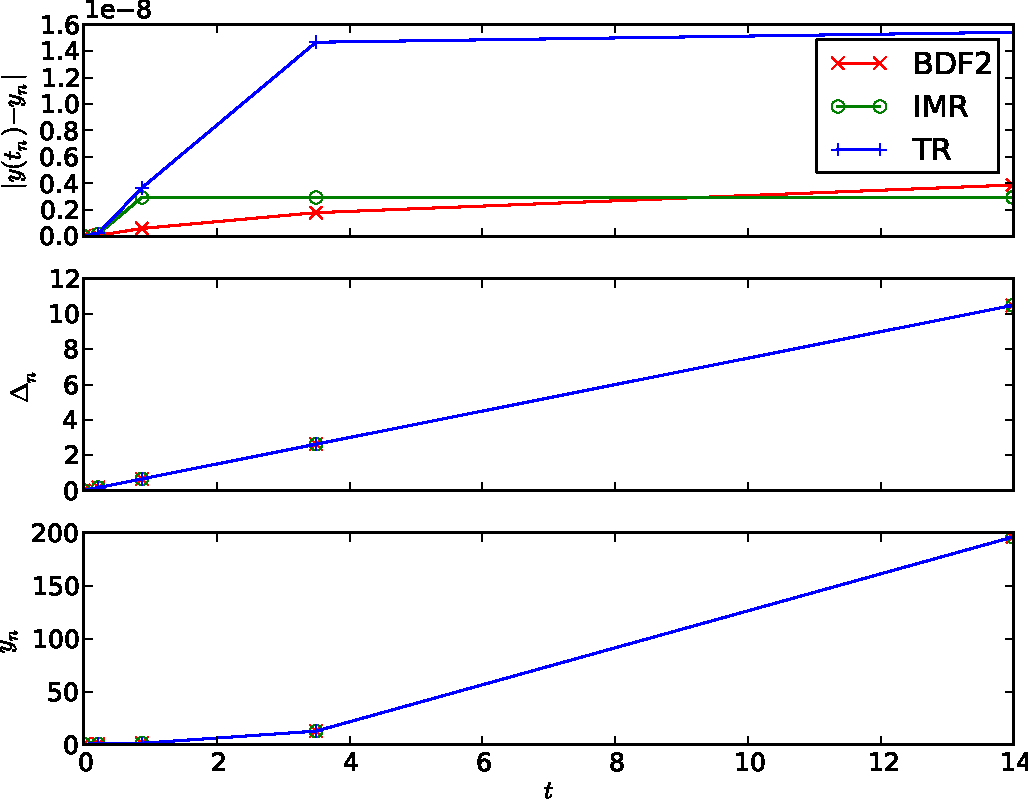
\includegraphics[width=1\textwidth]{plots/aimr_odes_traces/poly2-errornormsvs-dtsvs-tracevaluesvstimes}
  \caption{Absolute error, time step size and computed solutions for the example ODE with exact solution $y(t) = t^2 + 0.5$.}
  \label{fig:imr-poly2-example}
\end{figure}


\subsection{A damped oscillatory example}
\label{sec:oscill-damp-example}

The next test features a damped oscillatory solution, the ODE is
\begin{equation}
  \label{eqn:imr-test-osc-damp}
  \begin{aligned}
    f(t,y) &= - \beta e^{-\beta t} \sin(\omega t) + \omega e^{-\beta t} \cos(\omega t), \\
    y(0) &= 0.
  \end{aligned}
\end{equation}
with the solution
\begin{equation}
  y(t) = e^{-\beta t} \sin(\omega t).
\end{equation}
The adaptive algorithm should produce time steps that oscillate in time with the truncation error, while at the same time gradually increase as the term $e^{-\beta t}$ goes to zero.

\begin{figure}
  \centering 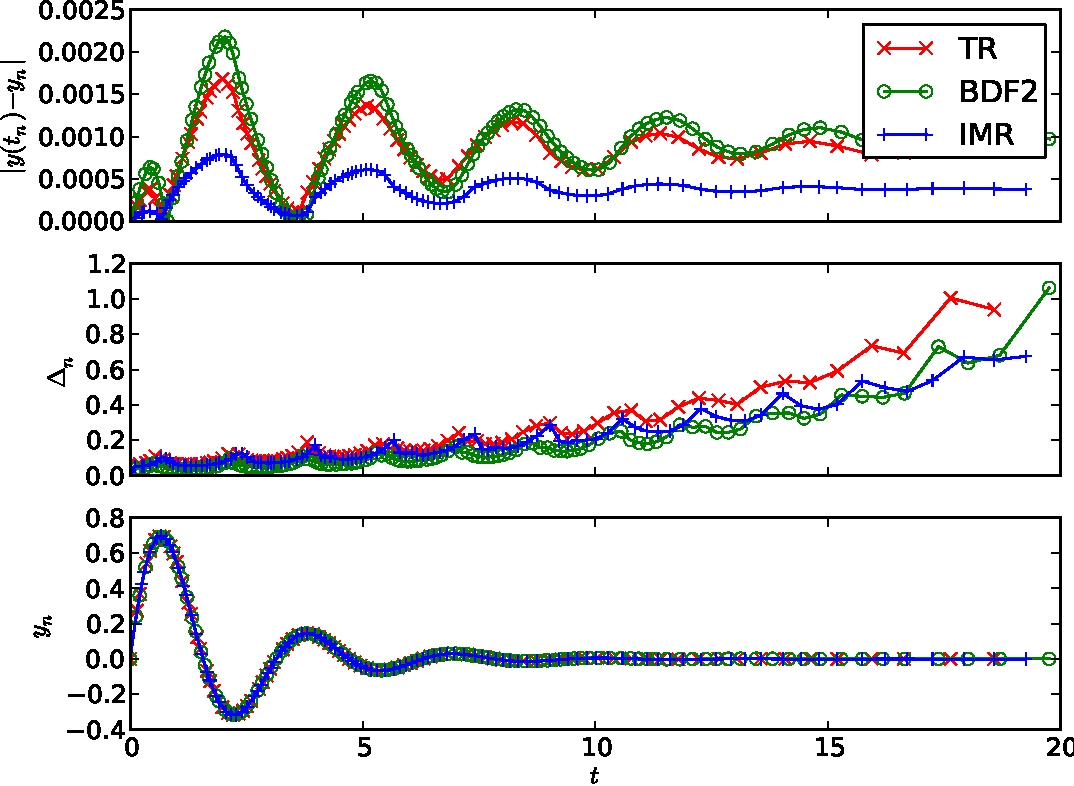
\includegraphics[width=1\textwidth]{plots/aimr_odes_traces/damped_oscillation-errornormsvs-dtsvs-tracevaluesvstimes}
  \caption{Absolute error, time step size and computed solutions for the oscillatory, damped example ODE with exact solution $y(t) = e^{-0.5t} \sin(2\pi t)$.}
  \label{fig:imr-osc-example}
\end{figure}

The ODE was solved with parameters $\omega = 2 \pi$ and $\beta = 0.5$, the results are shown in \cref{fig:imr-osc-example}.
All three methods have similar errors and time step sizes.
The IMR method chooses slightly smaller steps than TR (which explains the slightly lower error magnitudes).
BDF2 has the worst errors as expected because the coefficient of the main LTE term is the largest (see \cref{sec:deriv-local-trunc}).

Note that the plot shows the global error, whereas local truncation error estimates are used for step size selection calculations.
Hence the fact that the global error increases above the tolerance, $\toltt$, is not surprising.

Interestingly, there is a slight lag on the time step response of the IMR method as time steps become larger.
This could be due to the fact that IMR uses data from three previous steps in its LTE estimate, whereas the others only use two previous steps.

In \cref{fig:imr-osc-example-scatter} we show plots of the decrease in global error norm as the tolerance is decreased.
The consistent decrease in the error norms indicates that all of the adaptive methods are able to control the error in the expected manner.

\begin{figure}
  \centering 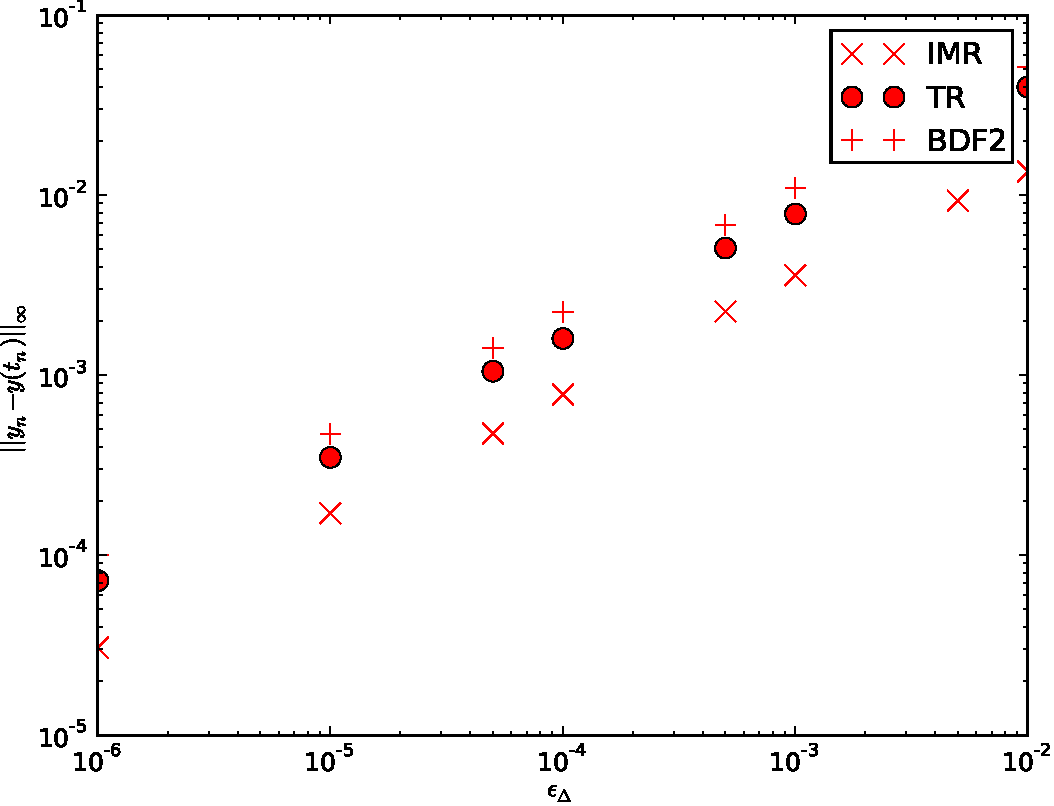
\includegraphics[width=0.8\textwidth]{plots/aimr_odes/damped_oscillation-maxoferrornormsvs-tol}
  \caption{Behaviour of the global error norm with varying tolerance for the oscillatory, damped example ODE with exact solution $y(t) = e^{-\beta t} \sin(\omega t)$.}
  \label{fig:imr-osc-example-scatter}
\end{figure}

\subsection{A stiff example}
\label{sec:imr-stiff-example}

We consider the stiff example ODE used in the definition of A-stability:
\begin{equation}
  \label{eqn:imr-test-stiff}
  \begin{aligned}
    f(t, \yv) &= -\lambda \yv, \\
    \yv(0) &= 1,
  \end{aligned}
\end{equation}
with the exact solution
\begin{equation}
  \label{eqn:imr-test-stiff-exact}
  \yv(t) = e^{-\lambda t}.
\end{equation}
This example will test that the single step of the eBDF method provides reliable LTE estimates even in cases where the problem is stiff.
The time steps should start small but rapidly increase as the exponential decays to zero.

The results of the applying the three methods to problem~\cref{eqn:imr-test-stiff} with $\lambda = 100$ and $\yv_0 = 1$ are shown in \cref{fig:imr-stiff-example}.
The behaviour of the IMR and BDF2 time integrators is essentially the same, indicating that our adaptivity algorithm is effective for stiff problems.
The time steps selected by the TR algorithm do not grow as fast as those selected for the other schemes at large $t$, this is probably due to the build-up of round-off error as noted in \eg \cite{Gresho2008}.

\begin{figure}
  \centering
  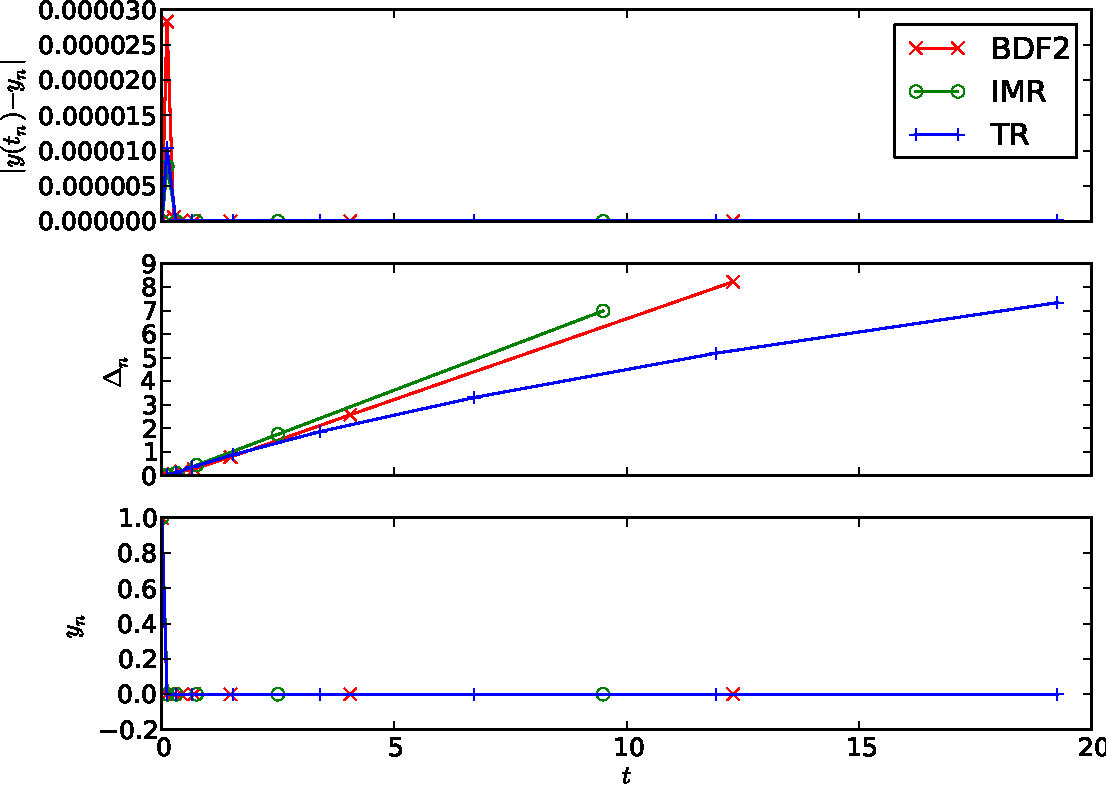
\includegraphics[width=1\textwidth]{plots/aimr_odes_traces/simple_stiff-errornormsvs-dtsvs-tracevaluesvstimes}
  \caption{Absolute error, step size and computed solutions for the stiff example ODE.}
  \label{fig:imr-stiff-example}
\end{figure}


\subsection{Order reduction example}
\label{sec:order-reduct-example}

\begin{figure}
  \centering  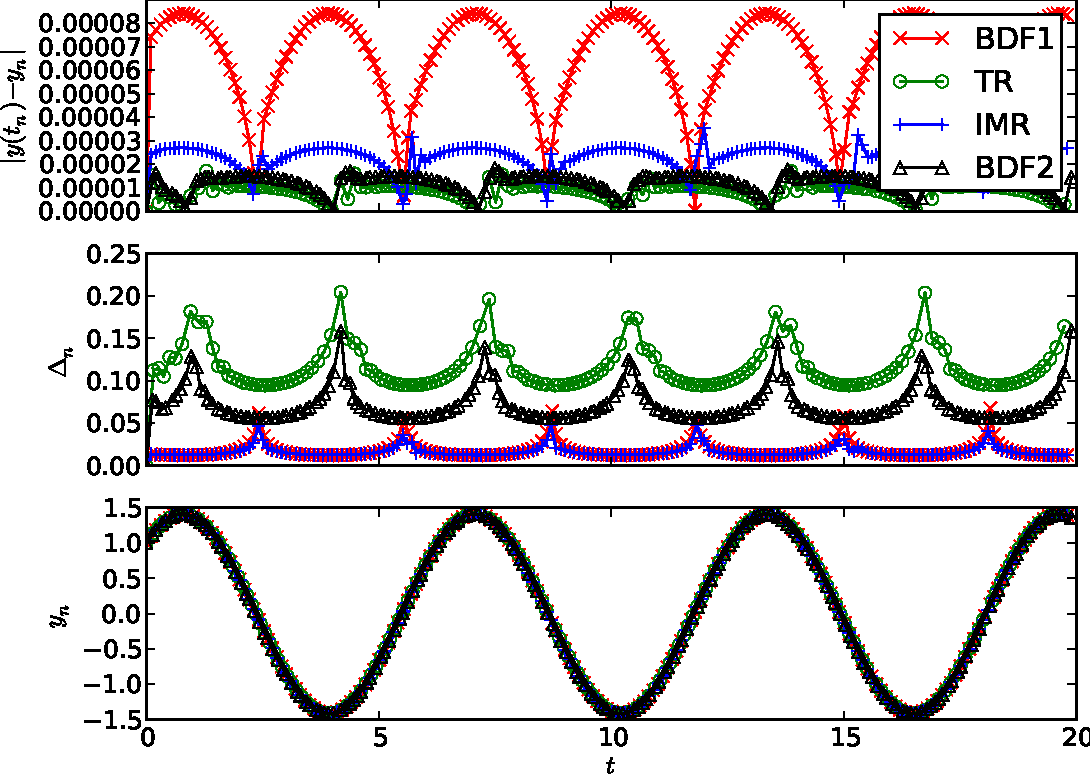
\includegraphics[width=0.8\textwidth]{plots/aimr_odes_traces/strong_order_reduction-errornormsvs-dtsvs-tracevaluesvstimes}
  \caption{Absolute error, step size and computed solutions for the stiff order reduction example ODE given in \cref{eqn:imr-test-order-reduction}.}
  \label{fig:imr-order-reduction-example}
\end{figure}

\begin{figure}
  \centering  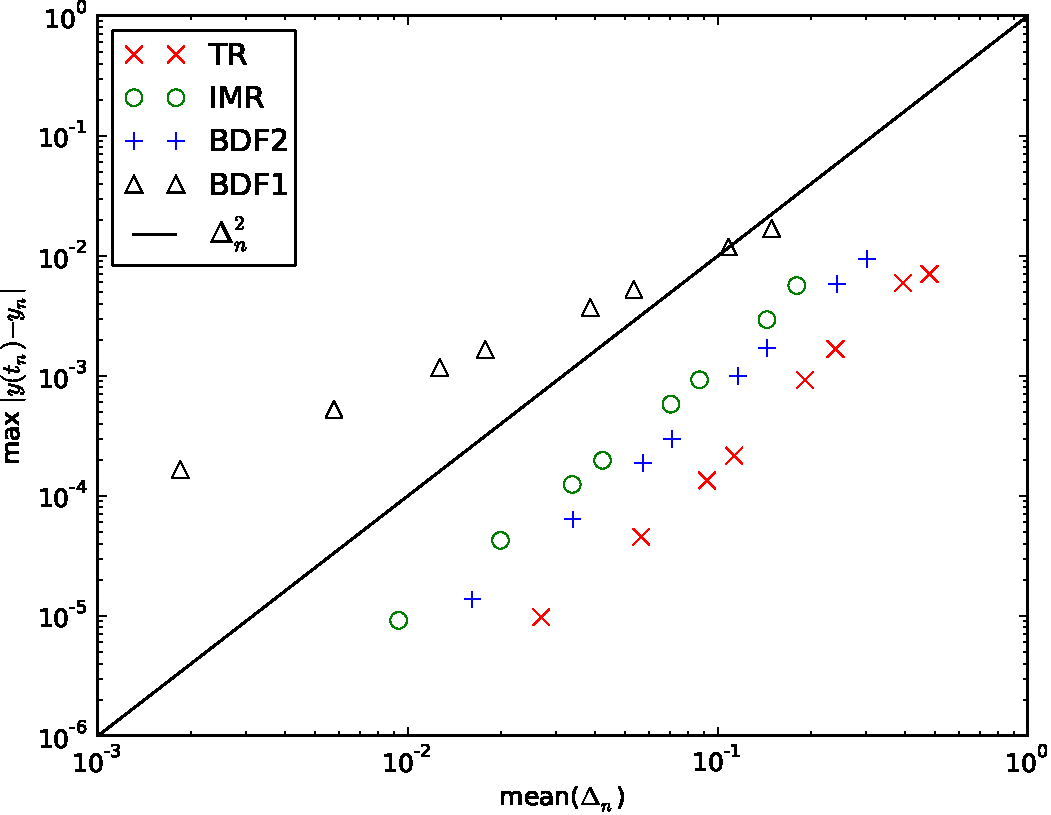
\includegraphics[width=1\textwidth]{plots/aimr_odes/order_reduction-maxoferrornormsvsmeanofdts.pdf}
  \caption{Behaviour of the global error norm with varying tolerance vs mean step size for the order reduction example.}
  \label{fig:imr-order-reduction-convergence}
\end{figure}

The order reduction effect, discussed in \cref{sec:order-reduction}, should be automatically detected and adjusted for by a good adaptive time step selection algorithm.
So as a final example we study \cref{eqn:imr-test-order-reduction}, the test ODE for order reduction:
\begin{equation}
  \begin{aligned}
    f(t, y) &= -\lambda (y - g(t)) + g'(t), \\
    y_0 &= g(0),
  \end{aligned}
\end{equation}
with exact solution
\begin{equation}
  y(t) = g(t).
\end{equation}
For these experiments we chose an oscillatory function, $g(t) = \sin(t)$ and $\lambda = 100$.

Using \cref{eq:reduced-order-imr-truncation-error}, the dominant term of the LTE of IMR for the case when $\dtn \gtrsim 1/\lambda$ is
\begin{equation}
  \lte^\imr = \frac{\dtn^2}{4} \sin(\thf),
\end{equation}
for smaller $\dtn$ the $\dtn^3 \cos(t)$ term will gradually become more important.
Note that for TR and BDF2 $\lte \propto \dtn^3 \cos(t)$, while for BDF1 $\lte \propto \dtn^2 \sin(t)$.
Hence we expect to see the adaptive IMR perform similarly to BDF1, and to select much smaller time steps than TR and BDF2 in order to control the larger errors.
To test this we also run the experiment with an adaptive BDF1 (backwards Euler) method using Milne's device (with forward Euler) for adaptivity \cite[270]{GreshoSani}.

The results are shown in \cref{fig:imr-order-reduction-example}.
As expected the implicit midpoint rule selects time step sizes very similar to the first order BDF1 method due to order reduction.
This allows it to retain similar accuracies to the TR and BDF2 methods at the cost of requiring many more time steps.

The convergence of the solution as the adaptive integrator tolerance, $\toltt$, is reduced with fixed $\lambda = 100$ is shown in \cref{fig:imr-order-reduction-convergence}.
Note that IMR still displays second order convergence (albeit with much larger errors than TR or BDF2).
This is because we are not increasing $\lambda$ as we decrease $\toltt$, so we are measuring the normal convergence rather than B-convergence.

\FloatBarrier % Don't allow floats from last section into this one

\section{Numerical experiments with an ODE form of the LLG}
\label{sec:imr-ode-llg-numer-exper}
\sectionmark{ODE LLG experiments}


In \thisref{sec:imr-ode-llg-numer-exper} we present numerical experiments in which we apply the adaptive implicit midpoint rule algorithm to an ODE LLG problem.
As in \cref{sec:aimr-testing} we compare the performance of the adaptive IMR algorithm developed in \thisref{sec:adaptive-imr} with the adaptive TR and BDF2 algorithms (both with and without re-normalisation of the magnetisation after each step).
Experiments with PDE LLG problems are postponed until \cref{cha:numer-experiments}.

\subsection{Problem definition}
\label{sec:aimr-llg-problem-definition}

To avoid introducing a spatial discretisation we choose an example micromagnetic problem that can be modelled by an ODE: the reversal of a ``small'' spherical particle under spatially-uniform applied field.
With this geometry and with uniform initial magnetisation the magnetostatic field can be analytically shown to be $\hms = -\mv/3$ throughout the domain \cite[112]{Aharoni1996}.
This means that the magnetisation remains uniform for spheres small enough that the increase in exchange energy due to any non-uniformity is larger than the corresponding decrease in magnetostatic energy.

In this case the Landau-Lifshitz form of the Landau-Lifshitz-Gilbert equation \cref{eqn:nd-llg-full} reduces to
\begin{equation}
  \begin{aligned}
    (1 + \dampc^2) \dmdt &= - \mv \times \hv - \dampc \mv \times \bigs{\mv \times \hv}, \\
    \hv &= \happ + \kone (\mv \cdot \ev) \ev.
    \label{eqn:nd-ode-llg}
  \end{aligned}
\end{equation}

To simplify the problem even further we choose $\kone = 0$ and $\happ(t) = [0, 0, -H]$.
In this case an exact solution is available for the time taken for $\mv$ to reach a given angle to the $z$-axis, and for the amount of precession that will take place in that time, more details are given in \cref{sec:ellips-nano-part} or \cite{Mallinson2000}.\footnote{Actually the solution for the switching time can be easily extended to cases with $\kone \neq 0$ with $\ev = \unitz$ and/or to any $z$-aligned ellipsoid of rotation.
However it is harder to invert the solution to obtain $\theta(t)$ in these cases.}
The exact solution is best expressed in spherical polar notation:
\begin{equation}
  \begin{aligned}
    \theta &= \cos^{-1}(m_z/1),\\
    \phi &= \tan^{-1}(m_y/m_x),
  \end{aligned}
\end{equation}
where $\theta$ is the angle between $\mv$ and the $+z$-direction.
The time for a reversal, $\tau$, from the initial value $\theta_0$ to $\theta$ is given by
\begin{equation}
  \tau(\theta) = t_0 + \frac{\dampc^2 +1}{H \dampc}
  \ln \bigb{ \frac{\tan(\theta/2)}{\tan(\theta_0/2)} }.
  \label{eq:74}
\end{equation}
This allows us to calculate a (global temporal) error in the switching time:
\begin{equation}
  \swtimeerr_n = \abs{t_n - \tau(\theta_n)}.
  \label{eq:sw-time-error}
\end{equation}

Alternatively, \cref{eq:74} can be inverted to give $\theta$ as a function of time:
\begin{equation}
  \theta(t) = 2 \tan^{-1} \bigs{ \tan(\theta_0/2) \exp\bigb{\frac{tH\dampc}{\dampc^2 + 1}}}.
\label{eq:77}
\end{equation}
The azimuthal angle at a given $\theta$ is \cite{Mallinson2000}
\begin{equation}
  \varphi(\theta) = \phi_0 -  \frac{1}{\dampc} \ln \bigb{ \frac{\tan(\theta/2)}{\tan(\theta_0/2)} }.
\label{eq:78}
\end{equation}
After substituting \cref{eq:77} into \cref{eq:78} and cancelling terms we obtain
\begin{equation}
  \varphi(t) = \phi_0 - \frac{tH}{\dampc^2 + 1}.
  \label{eq:79}
\end{equation}
Hence we can also calculate a (global temporal) error in the magnetisation at time $t_n$
\begin{equation}
  \merr_n = \abs{\mv_n - \mv(t_n)},
\label{eq:m-sphere-error}
\end{equation}
where $\mv(t_n)$ is the Cartesian representation of \cref{eq:77}, \cref{eq:79}.

The appropriate choice of error norm $\swtimeerr$ or $\merr$ depends on the aim of the calculation.
We may simply want to find the switching time of the system, in this case the time error norm, $\swtimeerr$, is appropriate (and using time steps such that the precessional behaviour is fully resolved may be excessively expensive).
In other cases an accurate representation of the full behaviour of the system may be needed and $\merr$ is appropriate.

The only energy term able to vary for this problem is the Zeeman energy (the energy due to the
applied field), so the total energy is simply given by
\begin{equation}
  E = - \mv \cdot \happ = H m_z.
\end{equation}

For the main experiment we choose parameters $H = 1.1$ (sufficient to switch the magnetisation) and $\dampc = 0.01$ (a physically relevant value).
We set the initial magnetisation to be just off the $z$-axis in order to avoid the singularity in reversal time when $\theta_0 = 0$ (see \cref{eq:74}), more precisely we set $\mv_0 = (0.01, 0.0, 1.0)/\sqrt{1.0001}$.
The dynamics are simulated for 1000 time units for all experiments, which is sufficient time for the magnetisation to fully switch.
This experiment allows us to check the $\abs{\mv}$ conservation properties of the adaptive IMR, to compare the accuracy of the solution between different time integrators, and to check again the robustness of the time step selection algorithm.

We also run the same experiment with $\dampc = 0$.
This allows us to check the energy conservation properties of adaptive IMR and to observe the what effect the re-normalisation of the magnetisation has on the energy.
Note that with $\dampc = 0$ \cref{eqn:nd-ode-llg} becomes simply $\dmdt = - \mv \times \happ$, which is linear in $\mv$ and $t$, hence TR and IMR are identical for this example.



\subsection{Implementation details}

The implementation of the three time integration algorithms without the re-normalisation of $\mv$ is exactly as discussed in \cref{sec:aimr-implementation}.
We also test the performance of the TR and BDF2 methods with an added re-normalisation step to enforce constant $\abs{\mv}$.
The re-normalisation is done by simply replacing $\mv$ by $\mv/\abs{\mv}$, and is carried out at after every step (after the selection of the next time step to avoid complicating the step selection process).
In the experiments we compare the performance with and without re-normalisation where appropriate.

In the experiments below the Landau-Lifshitz form \cref{eq:ll-nd-llglike} of the LLG is used for ease of implementation.
Linearisation is carried out using the Newton-Raphson method.
Using the skew operator notation from \cref{sec:llg-jacobian} the Newton-Raphson residual for the Landau-Lifshitz form of the LLG is is
\begin{equation}
  \rv = (1 + \dampc^2) \dmdt + \skewm{\mv} \cdot \hv + \dampc \skewm{\mv}\skewm{\mv} \cdot \hv.
\end{equation}
The corresponding Jacobian can be easily derived using the methods discussed in \cref{sec:llg-jacobian} (note that here $\hv \neq \hv(\mv)$) and is given by
\begin{equation}
  \Jm = \pd{\rv}{\mv} = (1 + \dampc^2) J_{ts} \Idm_3 - \skewm{\hv} - \dampc \skewm{ \mv \times \hv }
  - \dampc \skewm{\mv} \skewm{\hv}.
\end{equation}

The $3 \times 3$ Jacobian is calculated analytically and inverted using a direct solve.
Unless otherwise specified the Newton tolerance is $\ntol = 10^{-12}$ (to obtain accurate geometric integration properties) and the adaptive integrator tolerance is $\toltt = 10^{-4}$.
The initial time step is $\dtinitial = 10^{-3}$ which is sufficiently small to allow the adaptive algorithm to naturally increase $\dtn$ to an appropriate value.


\subsection{Numerical results}
\label{sec:aimr-llgode-numerical-results}

\begin{figure}
  \centering
  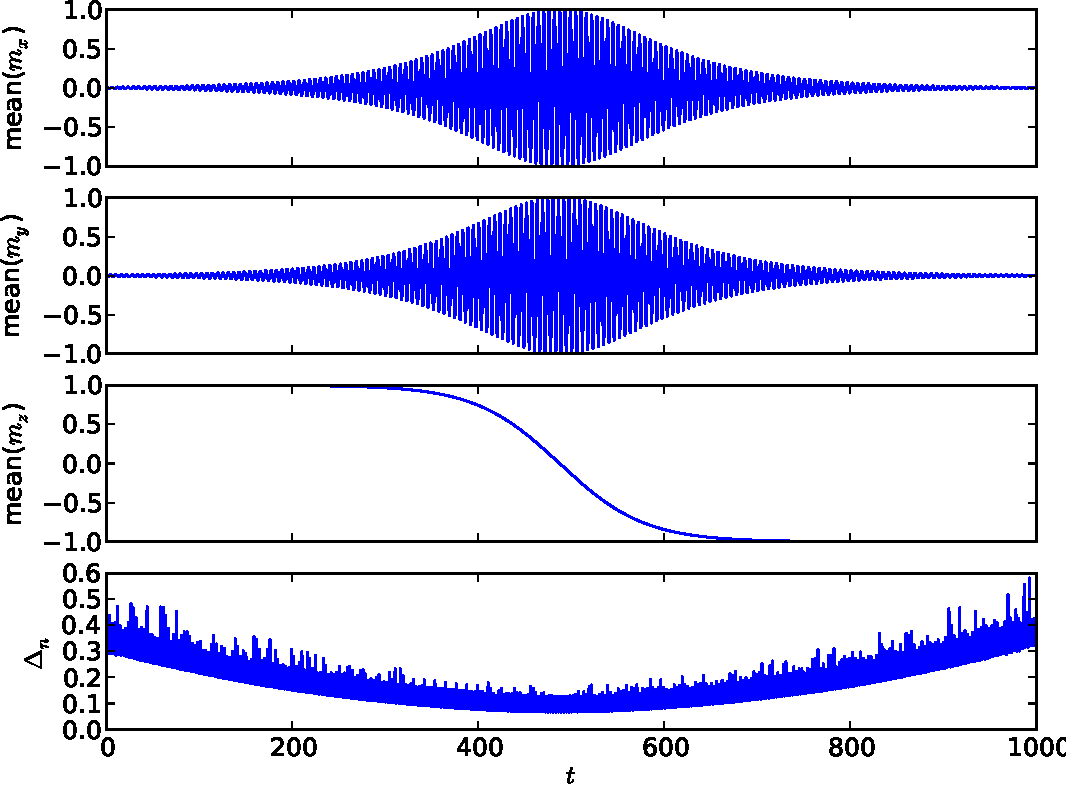
\includegraphics[width=0.8\textwidth]{plots/aimr-sphere-relax/imr0-meanmxsvs-meanmysvs-meanmzsvs-dtsvstimes.pdf}
  \caption{Plot of $\mv$ and $\dtn$ over time for the relaxing nano-sphere problem solved by adaptive IMR.}
  \label{fig:imr-llg-ode}
\end{figure}

The behaviour of the magnetisation and the time step selection using the adaptive IMR algorithm developed in \thisref{sec:adaptive-imr} is shown in \cref{fig:imr-llg-ode}.
The solutions given by adaptive BDF2 and TR (with $\abs{\mv}$ re-normalised after each time step)  are shown in \cref{fig:bdf2-llg-ode,fig:tr-llg-ode} respectively.
The overall behaviour of the IMR time step selection algorithm is seen to be working as expected: large steps are chosen at the start when very little switching occurs, the step size decreases as switching occurs and finally grows again as the switching finishes.

The small periodic peaks in the time step size are due to the precession: in Cartesian form (but not in the spherical polar coordinate form \cref{eq:79}) the precessional part of the solution is written as a sin/cosine term.
This causes periodic oscillations in the LTE.

Note, from \cref{fig:bdf2-llg-ode}, that the switching time obtained by BDF2 with the same error tolerances is very different to that given by IMR or TR.
This is due to BDF2's spurious numerical damping (see \cref{sec:numerical-damping}), which initially moves the solution towards the unstable fixed point at $\mv=[1, 0, 0]$.
The TR solution is qualitatively good.
The time steps selected by the three algorithms are similar, TR selects slightly larger steps as would be expected due to its lower local truncation error (see \cref{sec:deriv-local-trunc}).


\begin{figure}
  \centering
  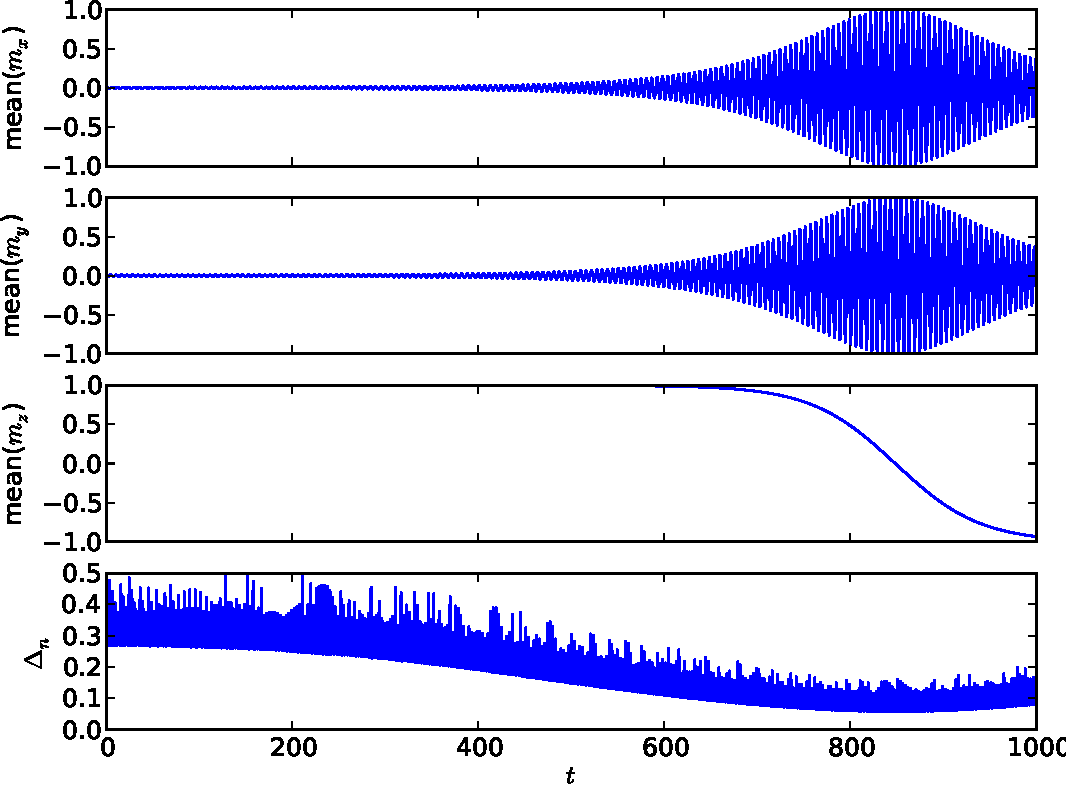
\includegraphics[width=0.8\textwidth]{plots/aimr-sphere-relax/bdf21-meanmxsvs-meanmysvs-meanmzsvs-dtsvstimes.pdf}
  \caption{Plot of $\mv$ and $\dtn$ over time for the relaxing nano-sphere problem solved by adaptive BDF2.}
  \label{fig:bdf2-llg-ode}
\end{figure}


\begin{figure}
  \centering
  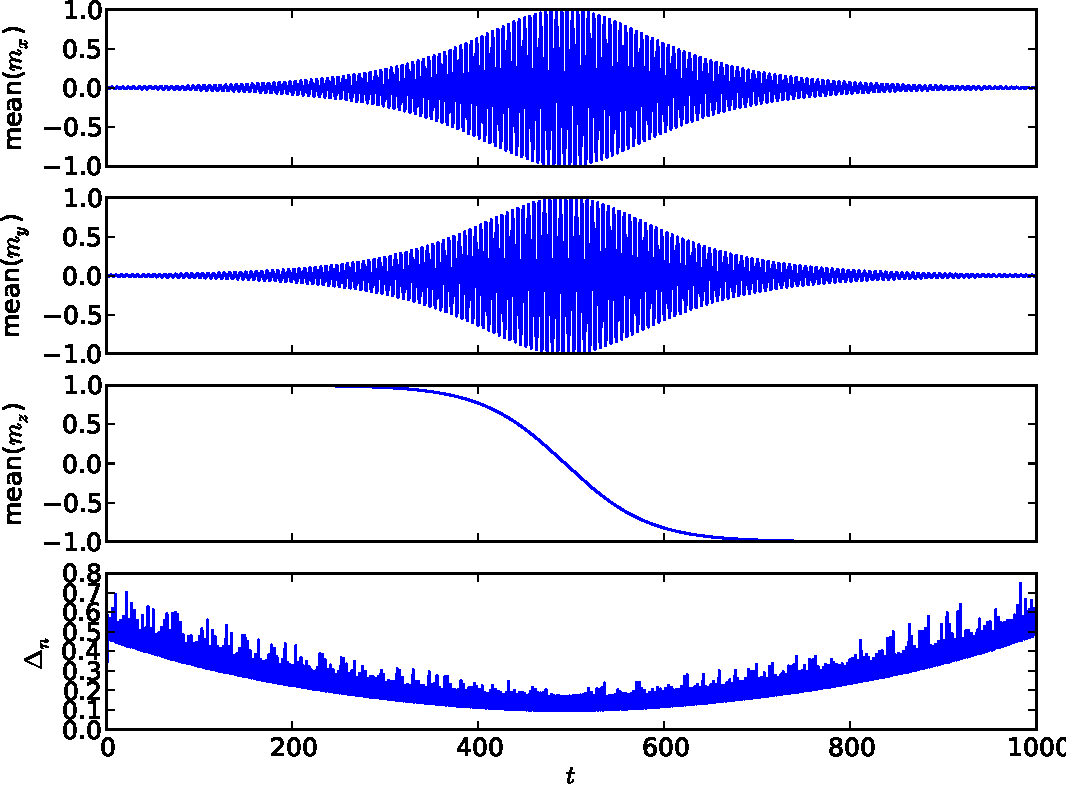
\includegraphics[width=0.8\textwidth]{plots/aimr-sphere-relax/tr1-meanmxsvs-meanmysvs-meanmzsvs-dtsvstimes.pdf}
  \caption{Plot of $\mv$ and $\dtn$ over time for the relaxing nano-sphere problem solved by adaptive TR.}
  \label{fig:tr-llg-ode}
\end{figure}

The behaviour of the magnetisation length over time is shown in \cref{fig:ml-aimr-ode}, where we write
\begin{equation}
  \errml(t_n) =  \abs{\abs{\mv_{j,n}} - 1}.
\end{equation}
The maximum error when IMR is used is $\errml \approx 10^{-12}$, which is consistent with the Newton tolerance.
In contrast the error in the magnetisation length with the TR and BDF2 schemes reaches $\sim 10^{-2}$.

As mentioned in \cref{sec:weak-cons-absmv} we would expect to see some effect on the conservation properties when the accuracy of the linearisation method is varied.
In our implementation the Newton-Raphson method is used for linearisation, so the relevant measure of accuracy is the Newton tolerance, $\ntol$.
The obvious experiment to carry out would be to vary the Newton tolerance and examine how the error in $\abs{\mv}$ is affected.
However the Newton-Raphson method converges extremely quickly meaning that the final residual is often many orders of magnitude smaller than the tolerance, this would hide any correlation between the tolerance and the error.
Instead we plot the error against the \emph{actual} converged residual norm (specifically: the mean over all time steps of $\norm{\rv}_\infty$ after the Newton method has converged for that time step).
In order to generate a variety of converged residual norms we run the experiment with a range of parameters:  $\dampc=1, 0.1, 0.01$, $\toltt = 5\times 10^{-3}, 10^{-3}, 5\times10^{-4}, 10^{-4}, 5\times10^{-5}, 10^{-5}$ and $\ntol=10^{-12}, 10^{-10}, 10^{-8}, 10^{-6}$.
A scatter plot showing the error in the length against the mean (over time) of the converged Newton residual norm is shown in \cref{fig:ml-aimr-newton}.
We see that the magnetisation length conservation behaviour of IMR is well controlled by the Newton tolerance even with large variations in the adaptive time integrator tolerance and the damping parameter.

\begin{figure}
  \centering
  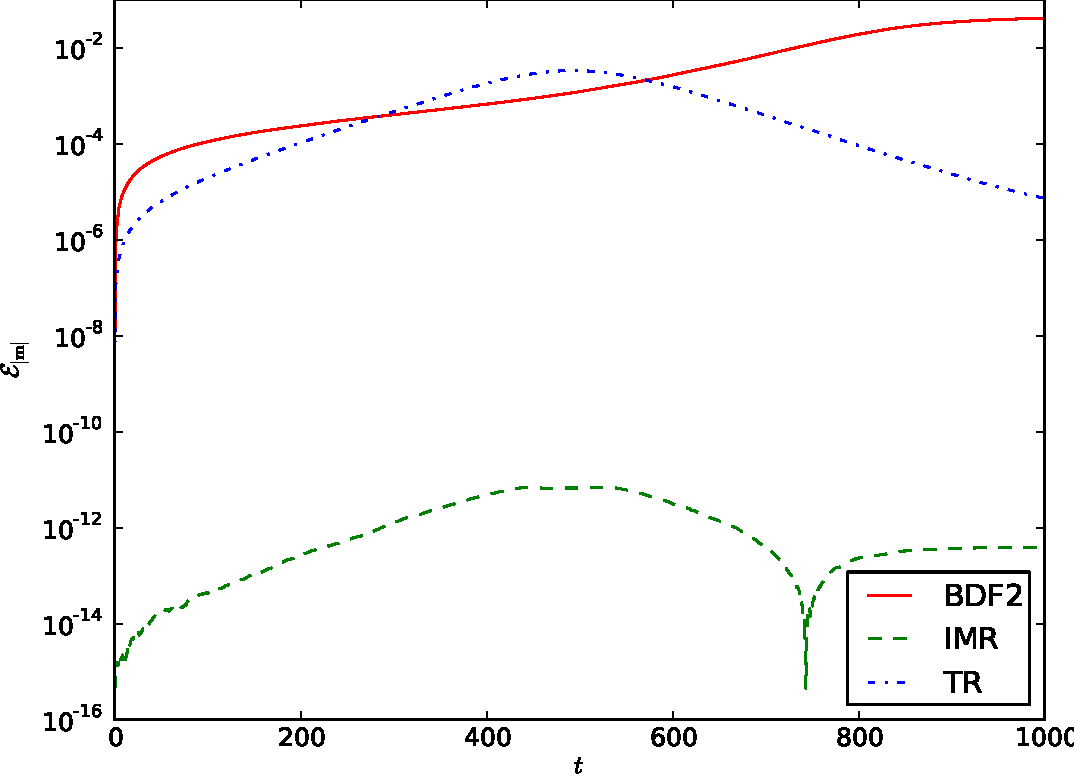
\includegraphics[width=0.8\textwidth]{plots/ode_llg_adaptive_ml/mlengtherrormaxesvstimes}
  \caption{Plot of magnetisation length errors, $\errml = \abs{\abs{\mv} -1}$, over time for the relaxing nano-sphere problem solved with each of the three adaptive integrators (without re-normalisation of $\mv$).}
  \label{fig:ml-aimr-ode}
\end{figure}

\begin{figure}
  \centering
  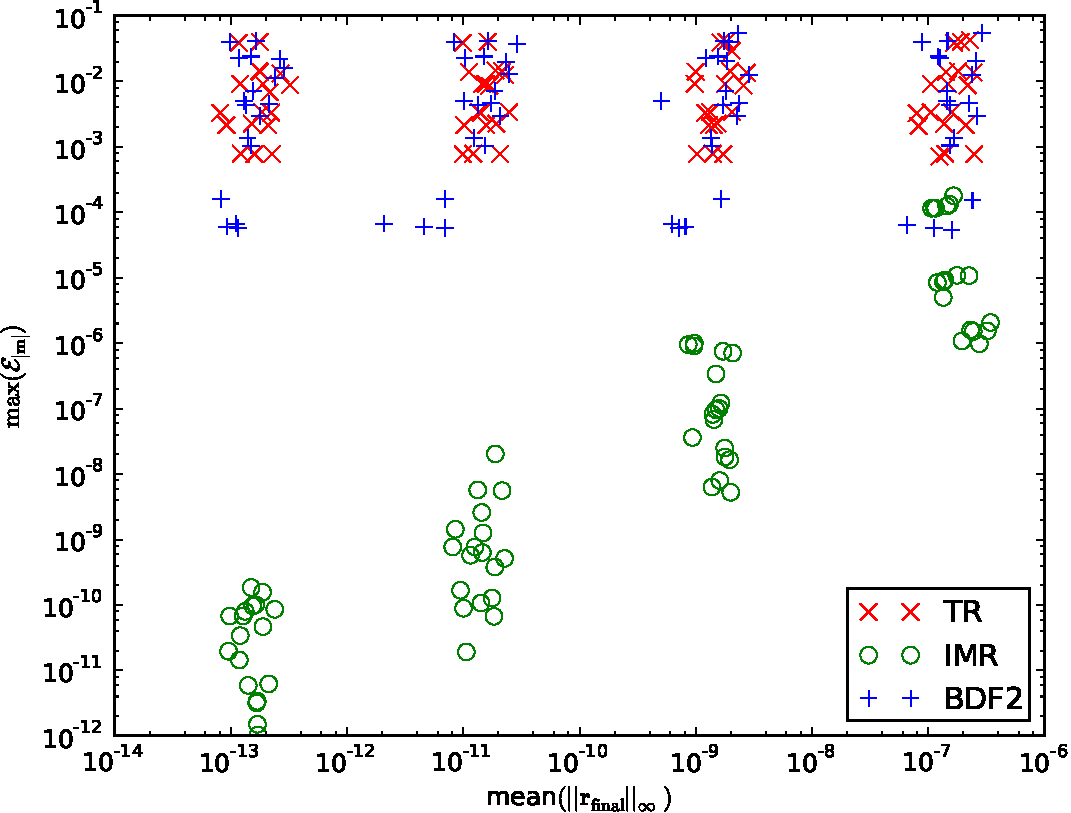
\includegraphics[width=0.8\textwidth]{plots/aimr_ode_llg_ml_sweep/maxofmlengtherrormaxesvsmeanminofnewtonresiduals.pdf}
  \caption{Plot of maximum magnetisation length error over time, $\max_n \abs{\abs{\mv_n} -1}$, against the mean converged Newton residual norm for the relaxing nano-sphere problem with a wide range of $\dampc$, $\ntol$ and $\toltt$ parameters.}
  \label{fig:ml-aimr-newton}
\end{figure}

The behaviour of the maximum error in the energy when $\dampc = 0$ as the adaptive step tolerance is reduced is shown in \cref{fig:energy-aimr-ode}.
The energy error for BDF2 without normalisation is around the Newton tolerance, but when re-normalisation is used the error in energy increases drastically.
This is due to the injection/removal of energy when the magnetisation length is modified.
The energy error when using the TR/IMR algorithm (recall that in this example TR and IMR are identical and renormalisation is not needed for either method due to the geometric integration properties) is below the minimum value that can be calculated using floating point arithmetic.
This is not surprising as we expect it to be significantly smaller than the energy error of BDF2, which is $\sim 10^{-14}$ and it is calculated as the difference of two values of $\order{1}$ (so it cannot be calculated if it is smaller than $\sim 10^{-16}$).

% I also tried it with larger precession (ie m further from z) to see if we can get big enough errors to see something interesting but nothing changes, leave it like this for simplicity.

\begin{figure}
  \centering
  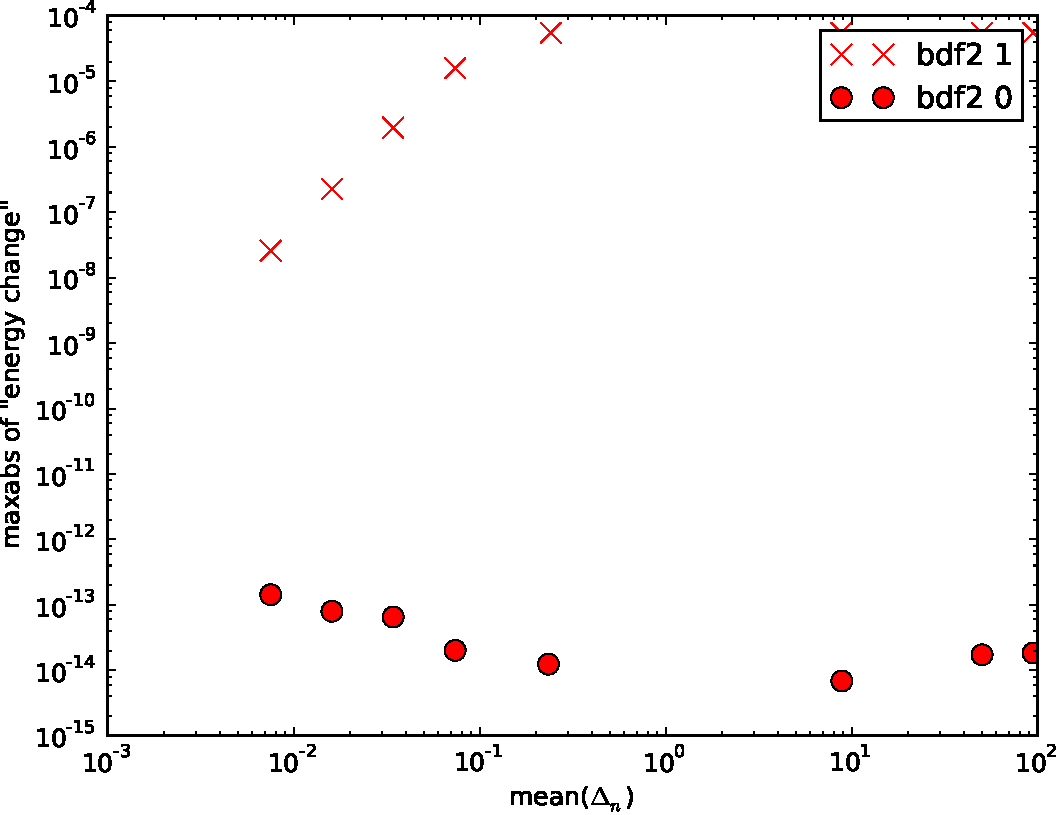
\includegraphics[width=0.8\textwidth]{plots/ode_llg_adaptive_energy/maxabsofenergychangevsmeanofdts}
  \caption{Convergence plot of the maximum error in the energy for the relaxing nano-sphere problem with $\dampc = 0$ solved using BDF2 with and without re-normalisation of $\mv$.
The energy error when using IMR is too small to be calculated.
The digit 1 or 0 in the legend indicates re-normalisation or no re-normalisation respectively.
}
  \label{fig:energy-aimr-ode}
\end{figure}

\begin{figure}
  \centering
  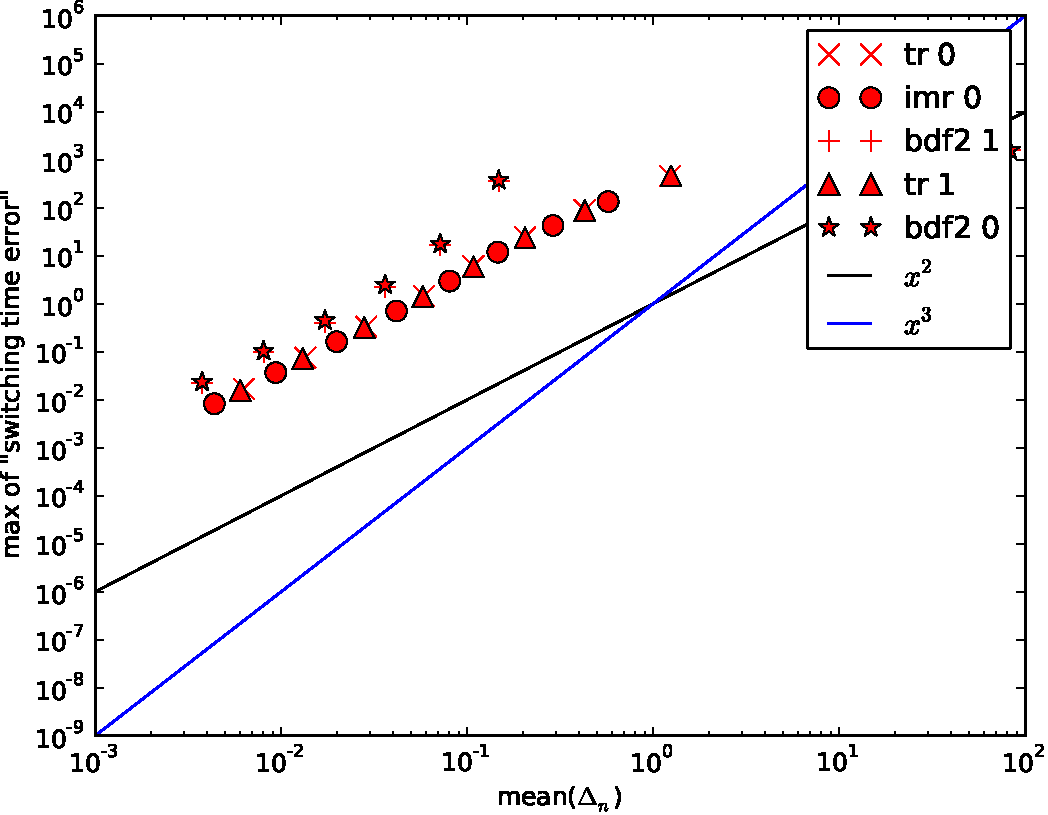
\includegraphics[width=0.8\textwidth]{plots/ode_llg_adaptive_convergence/maxofswitchingtimeerrorvsmeanofdts}
  \caption{Convergence plot of the switching time error, \cref{eq:sw-time-error}, against average time step for each method.
    The digit 1 or 0 in the legend indicates re-normalisation or no re-normalisation respectively.
}
  \label{fig:llg-ode-convergence-swtime}
\end{figure}


Finally, we show convergence plots with respect to the two error norms.
\Cref{fig:llg-ode-convergence-swtime,fig:llg-ode-convergence-m} show the convergence with respect to the switching time error, $\swtimeerr$, and the global error, $\merr$, respectively.
Adaptive TR and BDF2 algorithms both with and without re-normalisation of the magnetisation after
each step are shown, along with the adaptive IMR algorithm developed in \thisref{sec:adaptive-imr}.


In \cref{fig:llg-ode-convergence-swtime} the convergence (in $\swtimeerr$) rates for TR and IMR are flat consistent with the asymptotic predictions, in contrast BDF2 does not attain this asymptotic convergence state until a comparatively small time step.
The maximum errors are around $1000$ time units, a relative error of $\sim 100\%$.
The errors of TR and IMR are extremely similar for a given mean time step size.
Once the asymptotic convergence regime is reached BDF2 has roughly three times the error of the other methods.
Note that the re-normalisation of $\mv$ in BDF2 and TR has only a minimal effect on their global error.
This indicates that length conservation property of IMR is unlikely to be providing a major benefit to the global error in this simple example.


In \cref{fig:llg-ode-convergence-m} all convergence (in $\merr$) rates show a kink around $\mean(\dtn) = 0.1$.
This is because $\abs{\mv} \approx 1$ is fixed so the error norm $\merr$ cannot be worse than the anti-parallel case.\footnote{A more effective error norm for such large error cases would be to use polar coordinates and track the total azimuthal angle passed through. However this is non-trivial to implement in general and some rescaling would be required to prevent the $\varphi$ error from dominating.}
Above the kink the azimuthal angle is inaccurate and the error norms are meaningless, below the kink the usual convergence behaviour can be seen.
Comparing the error norms different methods we see the same relationships as in \cref{fig:llg-ode-convergence-swtime}: BDF2 has three times the error and re-normalisation has little effect.


Note that TR consistently chooses larger time steps than IMR despite having similar global errors.
This may indicate that the LTE of IMR is indeed larger than that of TR (as is expected), but that the geometric integration properties of IMR reduce the build up of global error.
Alternatively it may be due to differing accuracies in the LTE estimate.


% Note that there are fewer visible points on \cref{fig:llg-ode-convergence-swtime,fig:llg-ode-convergence-m} for BDF2 than the other two methods, this is because at larger tolerances BDF2 takes overly large time steps (and has large global errors to match).
% Hence some points for BDF2 do not fit on the same scale (for these missing points: $\mean(\dtn) \approx 10\dash 100$, $\swtimeerr \approx 1000$ \ie a relative error of $100\%$, $\merr \approx 2$).
% This is consistent with the qualitatively wrong results given by BDF2 in \cref{fig:bdf2-llg-ode}.

\begin{figure}
  \centering
  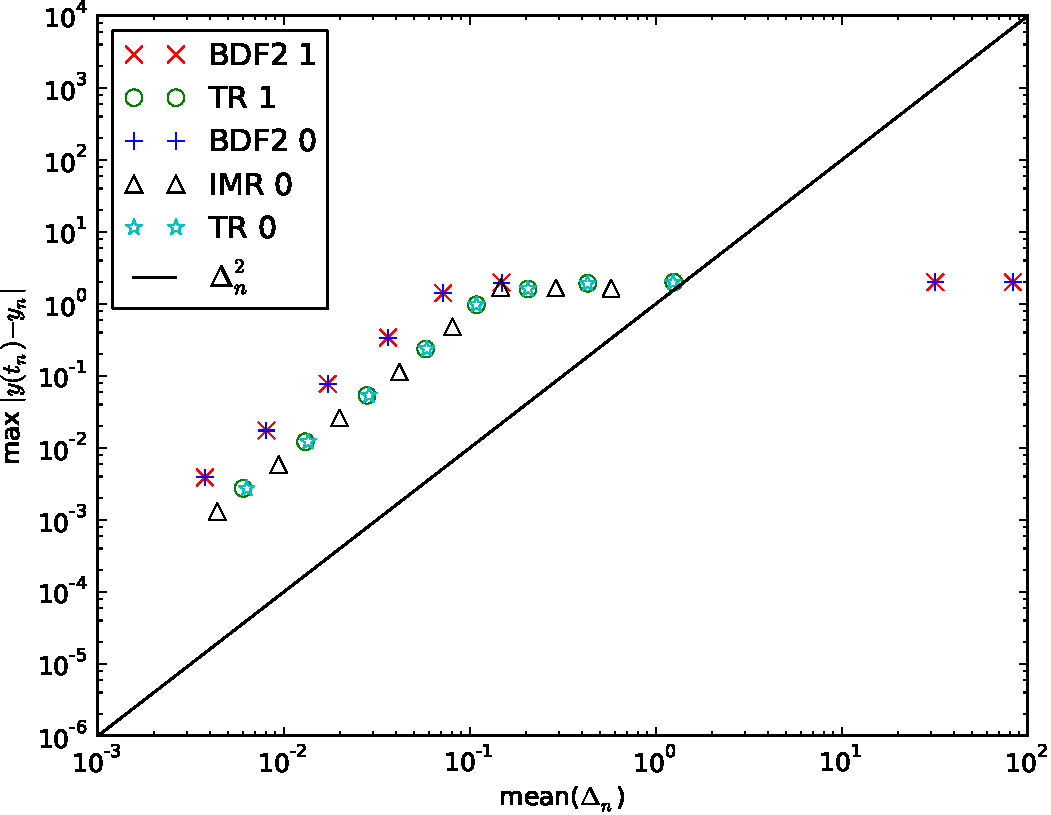
\includegraphics[width=0.8\textwidth]{plots/ode_llg_adaptive_convergence/maxoferrornormsvsmeanofdts}
  \caption{Convergence plots of the error in magnetisation, \cref{eq:m-sphere-error}, against average time step for each method. The digit 1 or 0 indicates re-normalisation or no re-normalisation respectively.}
  \label{fig:llg-ode-convergence-m}
\end{figure}

\section{Conclusions}

We have implemented an efficient algorithm for adaptive time step selection with the implicit midpoint rule.
The algorithm has been tested on a number of ODEs and found to follow the correct theoretically predicted step selection behaviour, and to behave similarly to other second-order adaptive time integrators.
We have also demonstrated robustness in stiff problems and correct behaviour even when order reduction phenomena are encountered.

When applied to an ODE form of the LLG the adaptive IMR algorithm conserves $\abs{\mv}$ as expected for a wide variety of parameters, but the example used here may be too simple for the energy property to be studied properly\footnote{Without damping the ODE form of the LLG is linear in $\mv$ and $t$ so TR and IMR are equivalent.}.
It also appears to give smaller global error norms than would be expected from its local truncation error, this may be due to the geometric integration properties.
Any effects of these geometric integration properties would be expected to be greatly amplified when solving ODE problems with many interacting spins or PDE problems.
This scenario will be tested in \cref{cha:numer-experiments} where the adaptive IMR algorithm is combined with the PDE methods discussed in other chapters.

Finally, we have observed some interesting results on the suitability of certain time integration methods to the simulation of the LLG equation.
We have found that the use of BDF2 results in significantly larger errors in the calculated switching time than the TR or IMR methods, particularly when the full precessional behaviour is not resolved.
We have also found that the process of re-normalising the magnetisation length after each time step in BDF2 methods greatly increases the error in the energy.


%%% Local Variables:
%%% mode: latex
%%% TeX-master: "./main"
%%% End:


\chapter{Stiffness of the LLG equation}
\label{cha:stiffn-llg-equat}


\section{Introduction}

Dynamic micromagnetic simulations  center around solving the Landau-Lifshitz-Gilbert (LLG) equation with various effective fields.
In this paper we focus on continuum mechanics models of micromagnetics, where the LLG with exchange becomes a system of partial differential equations (PDEs).
For such models stiffness (the restriction of time step size by stability rather than by the desired accuracy) has long been recognised as an issue, at least for some problems
\cite{Nakatani1989}.

Stiffness in PDEs has at least two possible sources:
firstly a problem may be physically stiff due to large differences in the characteristic time scales of different (physical) components of the solution \cite[Chap. 4]{Iserles2009};
secondly the choice of spatial discretisation method may cause stiffness.
In particular a fine spatial discretisation often results in a stiff system of ODEs.
An intuitive explanation for this is that a finer mesh resolves shorter wavelength modes, even if they have almost no effect on the resulting solution.
Shorter wavelength implies higher frequency, \ie shorter characteristic time scales.
These modes interact with the solution, and the large variation in time scales causes stiffness in a similar way to physical effects.
For a rigorous discussion of this effect in terms of the eigenvalues of the time integration operator see e.g. \cite[Sec 8.2]{Atkinson2009}.

As discussed in \cref{sec:time-discretisation} time integration methods can be roughly divided into two classes: those which are not good at solving stiff problems and those which are.
These two classes correspond to \emph{explicit} methods that calculate the value at the next time exclusively in terms of previous values and \emph{implicit} methods in which a system of equations must be solved.
Typically one step of an implicit method requires more computational effort than a step of an explicit method because of this solve.
However good implicit methods are unconditionally stable, allowing them to take much larger time steps when applied to stiff problems \cite[Chap. 4]{Iserles2009}.
Hence there is a trade-off between time step size and the computational effort per step.
Since the optimal choice depends on the stiffness it is important to understand its origins in micromagnetic simulations.

In \thisref{cha:stiffn-llg-equat} we examine numerically the relationship between stiffness and spatial discretisation size for a simple micromagnetic problem where stiffness due to physical effects can be ruled out.
We also explore how stiffness is affected by the use of the FEM/BEM method for magnetostatic calculations.
Finally, we study the effects of stiffness on methods which combine explicit magnetostatic calculations with implicit exchange field and LLG calculations (\ie semi-implicit methods).

\section{The model}

In these experiments we use the FEM discretisation of the non-dimensionalised LLG as discussed in \cref{sec:galerk-meth-llg}.
When in use magnetostatics are handled using the FEM/BEM discretisation as discussed in \cref{sec:hybr-finit-elem}.

\subsection{Implicit time integration}
For implicit integration we use the implicit midpoint rule (IMR) with constant time steps as discussed in \cref{sec:adaptive-imr}.
The complete problem (including the magnetostatic potential equations) is then linearised using Newton's method.
The resulting linear system is solved using GMRES with an incomplete LU decomposition\footnote{\hypre's Euclid preconditioner \cite{hypre} with no drop tolerance and factorisation level 1.} of the sparse parts of the system as a preconditioner, ignoring the dense block in the Jacobian arising from the BEM.

\subsection{Explicit time integration}
For the explicit integration we need to use an explicit rearrangement \cite[181]{Aharoni1996} of the LLG equation
\begin{equation}
  \label{eq:ll}
  \begin{aligned}
    \dmdt (1 + \dampc^2) &= - \mv \times \hv - \dampc \mv \times \left( \mv \times \hv \right).
  \end{aligned}
\end{equation}
As the time integrator we use a two stage Runge-Kutta method (RK2), also known as Heun's method:
\begin{equation}
  \label{eq:heunn}
  \begin{aligned}
    \mvtemp &= \mv_n + \dtn f(t_n, \mv_n), \\
    \mv_{n+1} &= \mv_n + \frac{\dtn}{2} \left( f(t_n, \mv_n) + f(t_{n+1},
      \mvtemp) \right).
  \end{aligned}
\end{equation}
Time derivatives are calculated within the Galerkin method by inverting the finite-element mass matrix using a diagonally preconditioned conjugate gradient solver.
The magnetostatic potential $\phim$ is recalculated using the FEM/BEM method at appropriate time and magnetisation values during each stage of \cref{eq:heunn}.
The Poisson solves required for the evaluation of the potentials $\phione$ and $\phim$ use a conjugate gradient solver preconditioned with algebraic multigrid\footnote{One V(1,1) cycle of \hypre's BoomerAMG preconditioner \cite{hypre} with Gauss-Seidel smoothing, CLJP coarsening and a connection strength threshold of 0.7.}.


\subsection{Semi-implicit time integration}
The semi-implicit time integration method (SIMR) used is the implicit midpoint rule combined with the semi-implicitisation discussed in \cref{sec:semi-implicit-bem}.


\section{The Test Case}

As our example problem we chose a sphere with a radius of one exchange length.
The initial magnetisation is $\mv = [0.2, 0, 1.0]/|\mv|$, the applied field is $\happ =[0, 0, -1.1]$.
We considered three values for the Gilbert damping constant: $\alpha = 1, 0.1$ and $0.01$.
With this geometry and uniform magnetisation the magnetostatic field can be analytically shown to be $\hms = -\mv/3$ throughout the domain \cite[112]{Aharoni1996}, and so, due to energy considerations, the magnetisation remains uniform for spheres of radius $R < 2.082 \sqrt{3} \sim 3.606$ exchange lengths \cite[211]{HubertSchafer}.
??ds repeated from \cref{sec:imr-ode-llg-numer-exper}

% Note that analytically the magnetostatic field has no effect on the dynamics because it is always anti-parallel to $\mv$ (the cross product of anti-parallel vectors is zero).
The dynamics are therefore very simple: the magnetisation processes around the $z$-axis while gradually damping towards the applied field (along the negative $z$-axis).
This simplicity means that the problem can also be written as an ODE, allowing for useful comparisons.
Additionally exact solutions for the switching time are known \cite{Mallinson2000}, allowing quantification of the error.

Good quality (radius-to-edge ratio $ > 2$) quasi-uniform unstructured tetrahedral meshes were generated using TetGen \cite{tetgen-website}. Meshes were refined by decreasing the maximum element volume parameter.

All simulations were run for 4 time units ($\approx 20\text{ps}$) with a full reversal taking between 8 and 400 time units depending on the damping.
We ran the experiment without magnetostatics, with FEM/BEM magnetostatics and with the analytical magnetostatic field for each value of the Gilbert damping constant.

We use a simple heuristic algorithm to find bounds for the maximum stable step size, $\dtmax$: The computation is repeated with a sequence of decreasing step sizes (halved each time) until a stable solution is observed, with step size $\dtx{a}$. A solution is considered to be unstable if at any node $|\mv| \neq 1$ or if the maximum angle between the magnetisation of neighbouring nodes is greater than $\pi/4$. The initial step size, $\dtinitial$ is selected such that the temporal error is sufficiently small (so that any reduction in step size below this value is wasteful).

This provides bounds on the maximum stable step of $\dtmax \in [\dtx{a}, 2\dtx{a})$. To tighten these bounds we then use two steps of a standard binary search algorithm: the computation is run with $\dtn{} = 3\dtx{a}/2$, if it is successful then $\dtmax \in [\frac{3\dtx{a}}{2}, 2\dtx{a})$ otherwise $\dtmax \in [\dtx{a}, \frac{3\dtx{a}}{2})$.

% The spherical mesh is generated using a face splitting algorithm: begin with an icosahedron (a polygon with 20 triangular faces) then divide each face into three triangles and move the newly created node onto the surface of the sphere.
% Repeat the division to generate progressively more accurate (and expensive) approximations to the surface of a sphere.
% The list of faces is then used as input to tetgen \cite{tetgen-website} to generate an unstructured tetrahedral mesh.

As mentioned above, the simple geometry of this problem means that the physics can be captured by an ODE version of the LLG:
\begin{equation}
  \label{eq:ode-llg}
  \begin{aligned}
    \dmdt (1 + \dampc^2) &= - \mv \times \hv - \dampc \mv \times \left( \mv \times \hv \right), \\
    \hv &= \happ - \mv/3,
  \end{aligned}
\end{equation}
where $\mv = \mv(t)$.

To assess physical stiffness and find a suitable $\dtinitial$ we solved \cref{eq:ode-llg} using the RK2 and IMR methods detailed above with $\dtx{} = 0.1$.
Using IMR with $\alpha = 0.01$ we found a relative error in the final switching time of $0.3\%$ (absolute error  $1.2 \text{ time units} \approx 6\text{ps}$), for other values of $\alpha$ the percentage error is even smaller.
The relative error in switching time with $\alpha = 0.01$ using RK2 was $2.25\%$ (this order of magnitude error difference may be a testament to the accuracy of geometric integration \cite{DAquino2005}).
Since these results are from an ODE calculation the error is only due to the time integration, with no contributions from spatial discretisation.
Based on these results we conclude that $\dtinitial = 0.1$ gives a sufficiently small temporal error to be a reasonable maximum time step size.
Additionally, since no stability issues were seen for any value of $\alpha$, we conclude that any lack of stability in the PDE case must arise purely from the spatial discretisation rather than the underlying physics.

% and forward Euler needs dt=0.0001 to get comparable error!!


\section{Results}


\begin{figure}
  \centering
  \includegraphics[width=0.8\textwidth]{images/stability_disabled}
  \caption{Maximum stable time step against discretisation size for LLG without magnetostatics. Data points are the stable dt values found, error bars represent the range in which the largest stable time step is contained. The horizontal dashed line shows the time step where RK2 and IMR are equally efficient (IMR is more efficient when the maximum stable step of the RK2 method moves below this line). The maximum time step is limited to 0.1 for accuracy reasons.}
  \label{fig:no-hms-stability}
\end{figure}


The results of the experiments with $\hms = \zerov$ are shown in \cref{fig:no-hms-stability}.
Results with full FEM/BEM magnetostatics and results with the analytical formula for magnetostatics are shown in \cref{fig:hms-stability} and \ref{fig:analytic-hms-stability} respectively.

In all cases we find that as the damping constant is reduced by an order of magnitude, stable explicit time step sizes are reduced by approximately a factor of two (due to an increase in the stiffness).

\begin{figure}
  \centering
  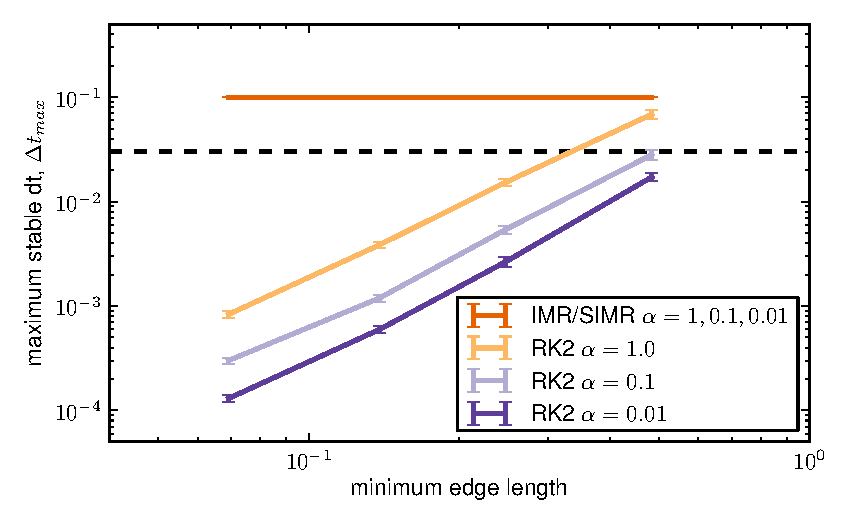
\includegraphics[width=0.8\textwidth]{images/stability_decoupled}
  \caption{Stable time step against discretisation size for LLG with FEM/BEM magnetostatics.}
  \label{fig:hms-stability}
\end{figure}


\begin{figure}
  \centering
  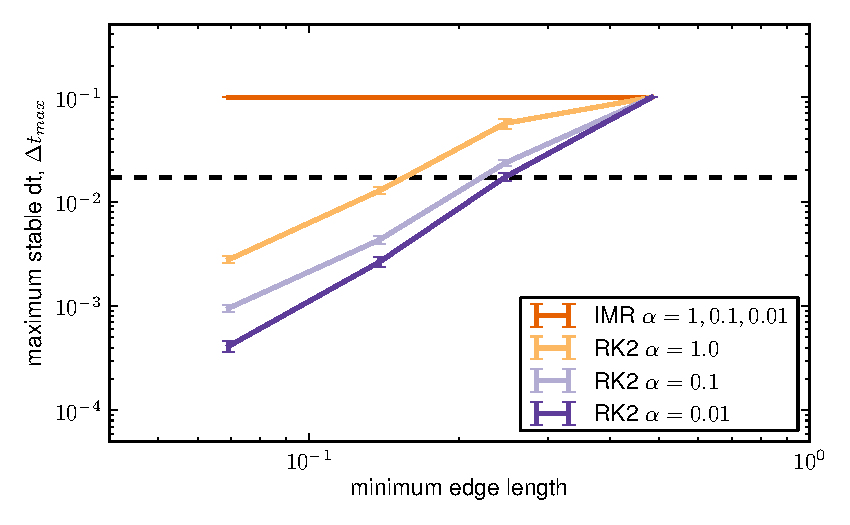
\includegraphics[width=0.8\textwidth]{images/stability_sphere}
  \caption{Stable time step against discretisation size for LLG with $\hv_{\text{ms}} = - \mv / 3$.
  }
  \label{fig:analytic-hms-stability}
\end{figure}

Comparing \cref{fig:no-hms-stability} and \ref{fig:hms-stability} we see that using FEM/BEM magnetostatics significantly increases the stiffness, requiring roughly an order of magnitude smaller explicit time steps.
However, from \cref{fig:analytic-hms-stability} we see that adding the exact field does not induce stiffness, so we can conclude that this effect is due to the FEM/BEM discretisation and not the magnetostatic field itself.
From our data we cannot predict whether other methods of calculating the magnetostatic field, such as multipole methods, will result in similar increases in the number of explicit time steps required.
However we expect that the effect is due to the coupling with the additional Poisson problems, thus any potential based method is likely to exhibit similar behaviour.

\cref{fig:hms-stability} shows that using a semi-implicit method with explicit magnetostatic calculations (SIMR) imposes no stability restrictions on the time step due to spatial discretisation for the spatial resolutions required for micromagnetic problems.

To further analyse our results we need an estimate of the ratio of computational effort for explicit vs implicit time steps. Without magnetostatics we find that each step of IMR takes on average 5.86 times more computation time than a step of RK2. With magnetostatics each step of SIMR only takes 3.40 times more computation time than a step of RK2 (the difference is due to the cost of solving multiple Poisson problems at each Runge-Kutta stage). Using these ratios we can calculate the stable RK2 time step required to have equivalent computational efficiency to IMR with step size 0.1. This stable step size is marked on \cref{fig:no-hms-stability}, \ref{fig:hms-stability} and \ref{fig:analytic-hms-stability} with a dashed line.

Based on these results we say that a problem is ``stiff'', and that an implicit method will perform significantly better than an explicit one, if the ratio of the desired time step, $\dtinitial$ to the maximum stable explicit time step, $\dtmax$ is greater than 20.
% This roughly agrees with the results of Suess \etal \cite{Suess2002}, who used the widely used (and presumably heavily optimised) CVODE package to solve the \mumag standard problem 4 using similar techniques to ours. % Their bdf2 steps are extremely slow, probably bad preconditioner.
A caveat is that both types of model could be further optimised using, for example parallelism, improved preconditioning, mass lumping, boundary matrix compression \cite[Sec. 3]{Knittel2011} etc.

Typical advice for the number of elements per exchange length is that an absolute minimum number is one, and in order to show that the results are mesh independent the mesh must be refined a few times \cite[Sec. 11]{nmag-manual}.
This leads to a reasonable finest mesh with around three elements per exchange length.

We see that with FEM/BEM magnetostatics, realistic damping ($\alpha = 0.01$) and at least three elements per exchange length the problem is stiff.

Without FEM/BEM magnetostatics stiffness only occurs if refinement to around five or more elements per exchange length is needed for any part of the domain.
Problems that require this level of refinement include resolving the geometry in studies of granular or patterned media \cite{Suess2002} and resolving vortex-core-like structures \cite{Andreas2014}.
% ??ds also \cite[App. D]{Knittel2011} found he needed this level of refinement for some parts of model to be accurate.

On the other hand LLG problems can be only moderately stiff if refinement is only needed up to the level of a few elements per exchange length, as is often required for simple geometries.
This is consistent with the fact that the mu-mag standard problem 4 is often solved using explicit integration methods with spatial refinement of around 0.5 exchange lengths \cite{mumag-website}.

Similar experiments with the standard 4th order Runge-Kutta method \cite[41]{Iserles2009} and $\alpha=1.0$ (plots not shown) give essentially the same results as for RK2. As $\alpha$ is reduced the maximum stable step size $\dtmax$ is reduced, but not as rapidly as for RK2. However due to the increased computational cost per time step (a factor of two) the onset of stiffness (for all $\alpha$) occurs at roughly the same spatial discretisation as for RK2 with $\alpha = 0.1$.

Finally we point out that the discussion above assumes that the accuracy obtained with $\dtx{} = \dtinitial$ is sufficient.
If higher accuracy than this is required then smaller time steps are needed regardless of stability, so the limitations imposed by stiffness are proportionally less significant.


\section{Conclusions}
Our results show that the LLG equation without magnetostatics or with analytical magnetostatic field calculations becomes stiff (\ie implicit methods are significantly more efficient) as the number of elements per exchange length decreases below around 5.
If FEM/BEM magnetostatic calculations are used stiffness occurs at much coarser discretisations, beginning at around $2\dash 3$ elements per exchange length.
In all cases decreasing the damping constant also increases the stiffness.

The results for the ODE version of the problem indicate that the observed stiffness is a result of the spatial discretisation and not the physics of the problem.
Since more complex physics is unlikely to reduce the stiffness, we expect that these results will extend to other, more complex, problems.

We also found that our semi-implicit FEM/BEM method does not suffer from discretisation induced stiffness.


%%% Local Variables:
%%% mode: latex
%%% TeX-master: t
%%% End:

\chapter{Validation, convergence and conservation experiments}
\chaptermark{Numerical experiments}
\label{cha:numer-experiments}

In this chapter we apply the various numerical methods constructed throughout this thesis to some micromagnetics problems.

The first case examined is a 2D problem without magnetostatics where there is a known wave-like analytical solution for certain initial conditions.
This allows us to test the convergence of the various discretisation approaches when applied to the LLG with the exchange effective field (\ie the PDE form).
It also allows us to test the geometric integration properties of the IMR for a simple PDE problem.

The second problem is another simple case, but with no analytical solution: a non-uniform applied field is used to induce non-uniform dynamics in a 2D problem without magnetostatics.
This allows us to test geometric integration properties of the IMR in the absence of an analytical solution.

Finally we show results for the \mumag standard problem \#4 \cite{mumag-website}, which is widely used to test dynamic micromagnetic codes.
This allows us to verify the complete model and to examine the geometric integration properties when FEM/BEM magnetostatics calculations are included.


\section{Example with a wave-like solution}
\label{sec:numer-exper}

\subsection{Problem definition}
\label{sec:wave-problem-definition}

In this experiment we solve a micromagnetic problem which has a wave-like exact solution in 2D.
The details of this solution are given in \cref{sec:wave-like-solution}.
We solve the LLG without magnetostatics on a two dimensional square domain $\magd = [0,1] \times [0,1]$ with periodic boundary conditions.
We integrate time over $T = [0, 5]$.
The solution is obtained by setting the initial condition according to \cref{eq:97}:
\begin{equation}
  \begin{aligned}
    m_x(0) &= \sin(c) \cos\bigb{\kvec \cdot \xv}, \\
    m_y(0) &= \sin(c) \sin\bigb{\kvec \cdot \xv}, \\
    m_z(0) &= \cos(c),
  \end{aligned}
\end{equation}
and using $\happ = \zerov$.
The solution parameters used are $\kvec = [2\pi, 2\pi]$ (so that the solution is periodic on domains of unit size), $c = 0.1\pi$, and $\dampc = 0.01$.
For the energy conservation experiments $\dampc = 0$ is used instead.

This example problem allows us to examine the convergence and geometric integration properties of IMR with the FEM using nodal quadrature.
In particular the existence of an exact solution allows us to easily measure the convergence rate for the various methods.


\subsection{Implementation details}
\label{sec:impl-deta}

We use the finite element method as discussed in \cref{sec:galerk-meth-llg} to spatially discretise the LLG equation.
Unless otherwise specified we use a mesh of square elements with $5 \times 2^4$ elements along each edge (1681 nodes in total).
For the evaluation of the resulting integrals both the nodal quadrature discussed in \cref{sec:local-nodal-integr} and standard Gaussian quadrature methods are used.

For time integration the adaptive IMR, TR and BDF2 methods are used with a tolerance of $\toltt = 10^{-5}$ and an initial time step of $\dtx{0} = 10^{-5}$ (significantly smaller than the time step selected by an initial experimental run).
Those methods which do not naturally conserve $\abs{\mv}$ (the TR and BDF2 methods, and IMR with Gaussian quadrature) are run both with and without re-normalisation of the magnetisation.
The re-normalisation process is implemented by setting each nodal value of the magnetisation to $\mv_i = \mv_i/\abs{\mv_i}$ after each time step (after the selection of the next step size to avoid complicating the adaptivity process).

Linearisation is handled using the Newton-Raphson method with Newton tolerance set to $\ntol = 10^{-12}$ (unless otherwise specified).
The resulting linear systems are solved using GMRES with an ILU(1) preconditioner as described in \cref{sec:llg-only-system,sec:linear-systems-probl-spec}.

The adaptive IMR integrator, as described in \cref{sec:adaptive-imr}, requires the computation of an explicit time step.
For this step we use the Landau-Lifshitz form of the LLG discretised in exactly the same way as described in \cref{sec:galerk-meth-llg}.
The resulting linear system (involving only a mass matrix) is solved using the method of conjugate gradients preconditioned by the lumped mass matrix (\ie the diagonal matrix of the row sums).
Note that when nodal quadrature is used the mass matrix is a diagonal matrix and no linear solve is needed (see \cref{sec:nodal-integration}).


\subsection{General results}

An example snapshot of the solution at time $t=0.1$ is shown in \cref{fig:2d-wave-snapshot}.
Over time the wave moves in the $[-1,-1]$ direction and is simultaneously damped out towards the $\mv = [0,0,1]$ state.

\begin{figure}
  \centering
  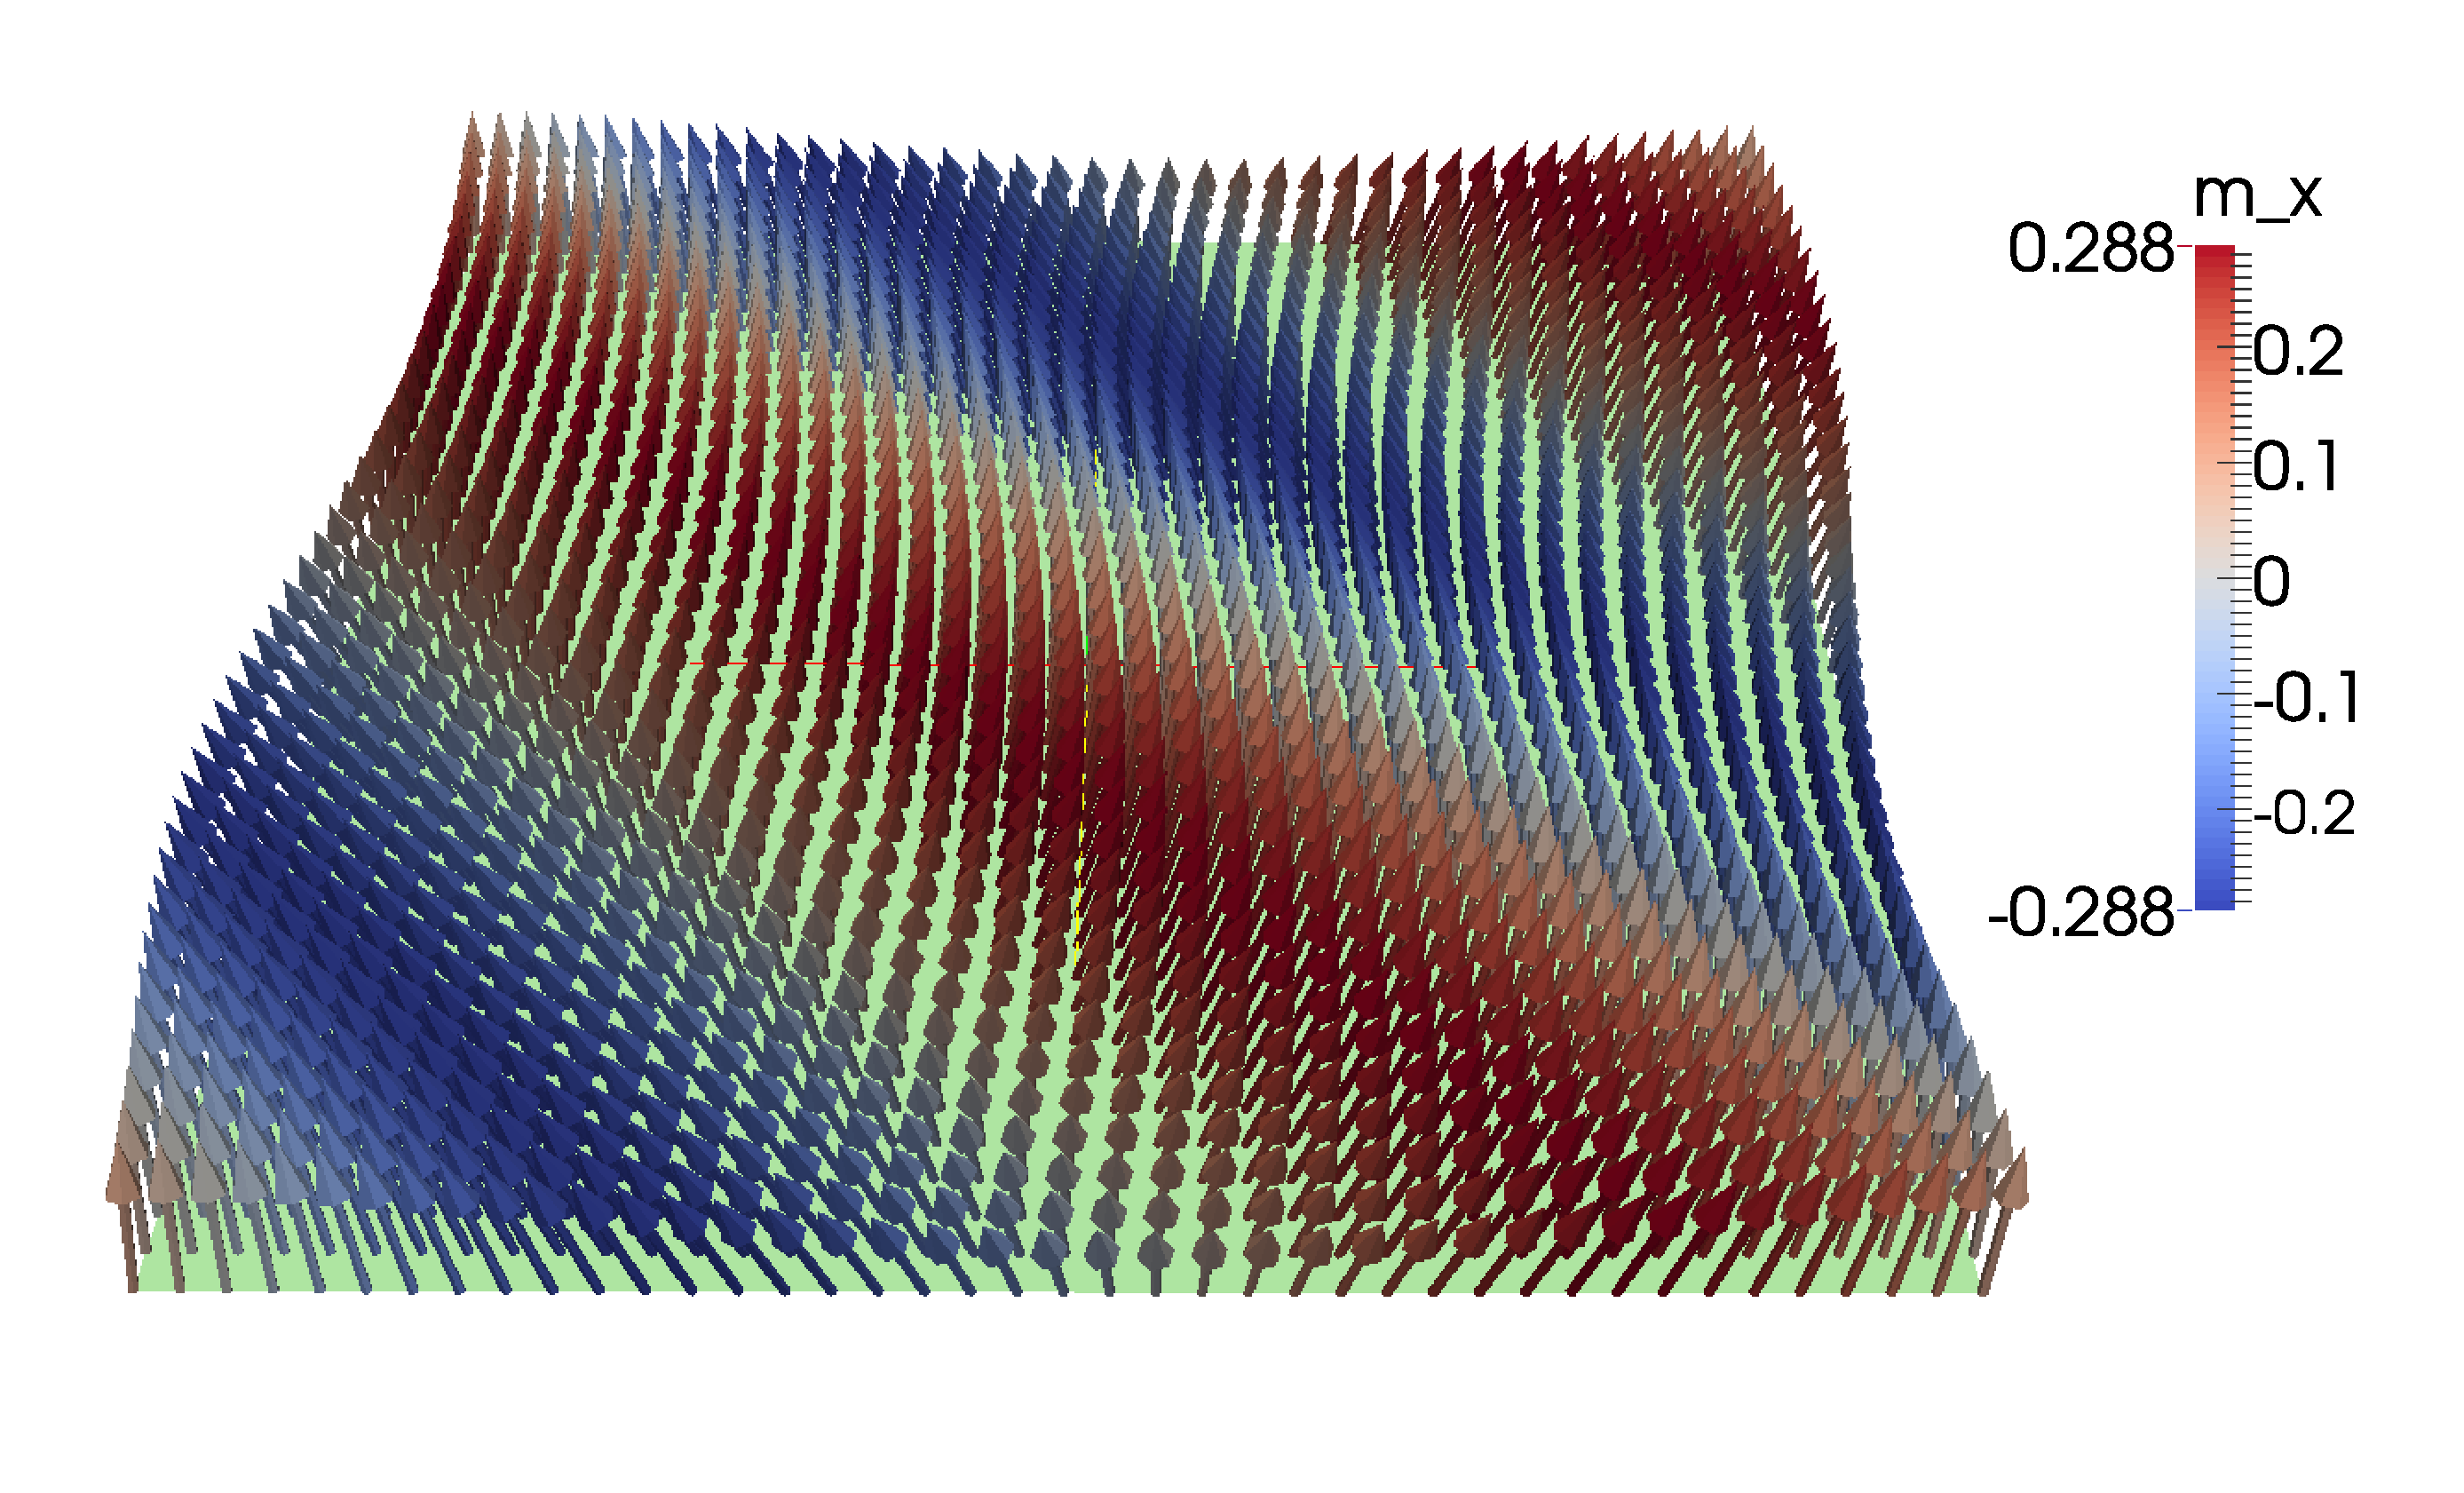
\includegraphics[width=0.8\textwidth]{images/2d_wave_picture_t0p1.pdf}
  \caption{Snapshot of the approximate solution for the 2D wave problem at $t=0.1$ time units obtained using adaptive IMR with nodal integration.
    Colour indicates the value of $m_x$.
    The $z$-component of the magnetisation is constant over the domain with $m_z = 0.958$.}
  \label{fig:2d-wave-snapshot}
\end{figure}

The behaviour of the approximate solutions over time at $\xv = \zerov$ is shown in \cref{fig:2d-wave-time-trace}.
Only results from the methods without re-normalisation are shown because they are identical to the equivalent method with re-normalisation (where applicable) at the scale of the plot.

The time steps selected by the various algorithms for this problem are also shown in \cref{fig:2d-wave-time-trace}.
The appearance of a jump in the time step size at $t=0$ is due to the algorithms rapidly increasing the time step size from the small initial value to a step size appropriate for the given tolerance.
After an appropriate step size is reached there is a smooth, gradual increase as the solution is damped out.

\begin{figure}
  \centering
  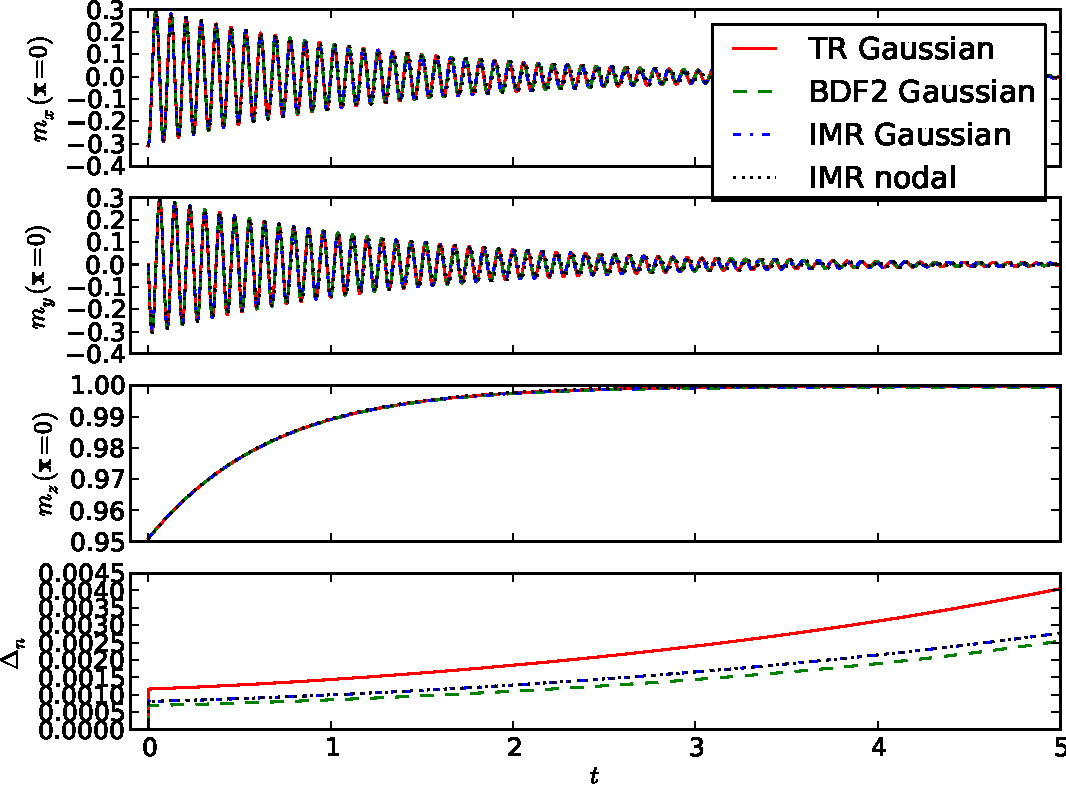
\includegraphics[width=0.9\textwidth]{plots/2d_wave_solution_time_trace/get2oftracevaluesvs-get3oftracevaluesvs-get4oftracevaluesvs-dtsvstimes.pdf}
  \caption{The temporal behaviour of the wave solution at $\xv = \zerov$ and the time step selected by the various adaptive integration schemes without re-normalisation.
    }
  \label{fig:2d-wave-time-trace}
\end{figure}


\subsection{Convergence study}

Since we have an exact solution for this example we can easily calculate an error norm and plot the convergence as both the time step $\dtn$ and the element edge length $h$ go to zero.
Following the example of Jeong \etal \cite{Jeong2014} we link the time step size to the spatial discretisation size by $\dtn = 0.32h$.
It is important to note that, in contrast to explicit time integration schemes, this coupling of the time and space discretisation parameters is \emph{not} required for stability.
It is merely more convenient to experiment with a single parameter than with two independent parameters.
We choose element edge lengths of $h = 1/(5 \cdot 2^n)$ with $n=1,2,3,4,5,6$.
% I tried n=7,8 but larger values of $n$ grow extremely computationally expensive for two reasons: firstly because we choose to reduce the time step and $h$ simultaneously, and so require more solves of larger systems.
% Secondly our iterative linear solver becomes less effective due to the extremely large systems involved ($\sim 10^6$ rows with $n=8$).

In these experiments we always use re-normalisation for schemes which are not expected to naturally conserve $\abs{\mv}$ because in practical applications such schemes would always use re-normalisation.

As a first convergence experiment we examine the norm of the error after a single time step
\begin{equation}
  \merr_{,1} = \norm{\mv(\xv_j, t_1) - \mv_{j,1}}_2.
\end{equation}
In this case we expect the convergence (in both space and time) to be second order for all methods.
The results of this experiment are shown in \cref{fig:convergence-one-step},
We see that convergence is indeed second order for all methods and that the accuracy of the BDF2 scheme is worse than the other schemes by a roughly constant factor.
We also see that the use of nodal quadrature results in an error increase by a small constant factor.
This indicates that the geometric integration properties of IMR with nodal quadrature give little or no benefit for a single time step, as would be expected.
\begin{figure}
  \centering
  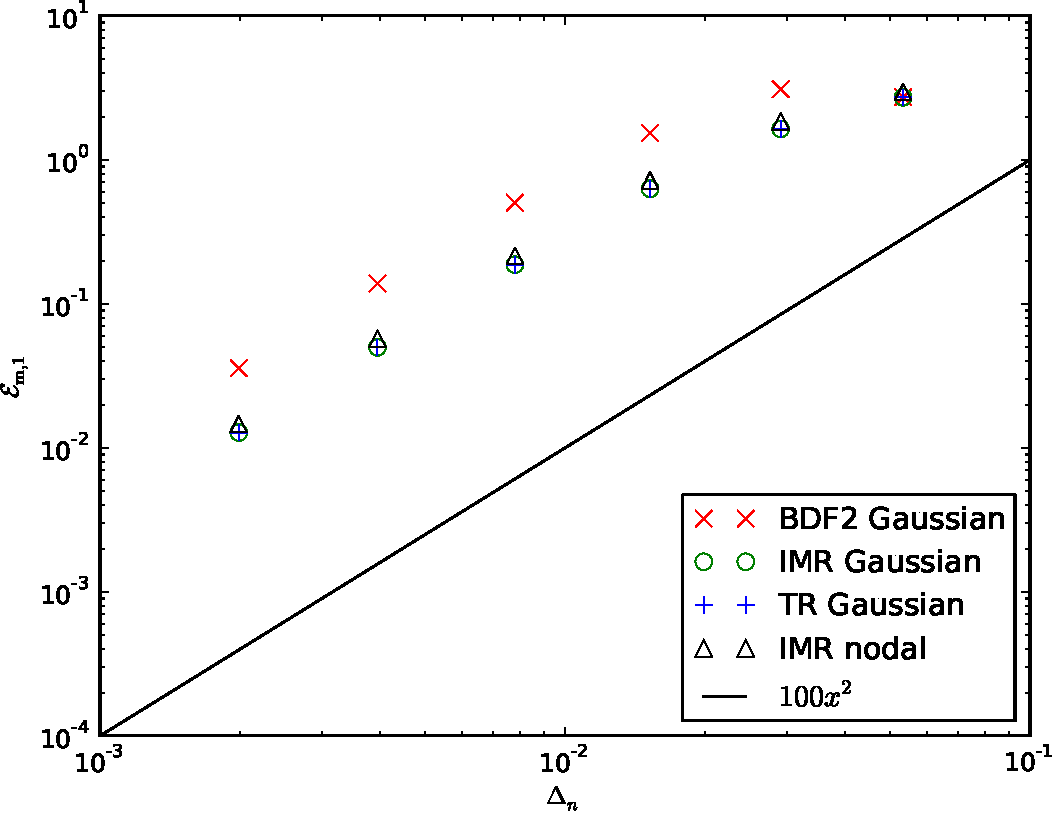
\includegraphics[width=0.9\textwidth]{plots/2d_wave_solution_convergence_long_time/firstoferrornormsvsfakemeanofdts.pdf}
  \caption{Convergence in the error norm $\errmpde{}$ after a single step of time integration for the 2D wave-like problem.}
  \label{fig:convergence-one-step}
\end{figure}



We also wish to examine a norm of the error after a large number of time steps, so for the rest of the experiments in this section we examine the integral of the error norm over $T = [0, 5]$.
However, reaching the levels of convergence required for $\errmpde$ to be meaningful is difficult because the ``worst case'' for the norm is that the approximated magnetisation is out of phase with the exact solution (\ie the error norm is bounded).
A plot of the time integral of $\errmpde$ is shown in \cref{fig:convergence-long-time-full-norm}.
No convergence is seen for IMR and TR until the spatial/temporal refinement level reaches $n=5$, and no convergence at all is seen for BDF2.
\begin{figure}
  \centering
  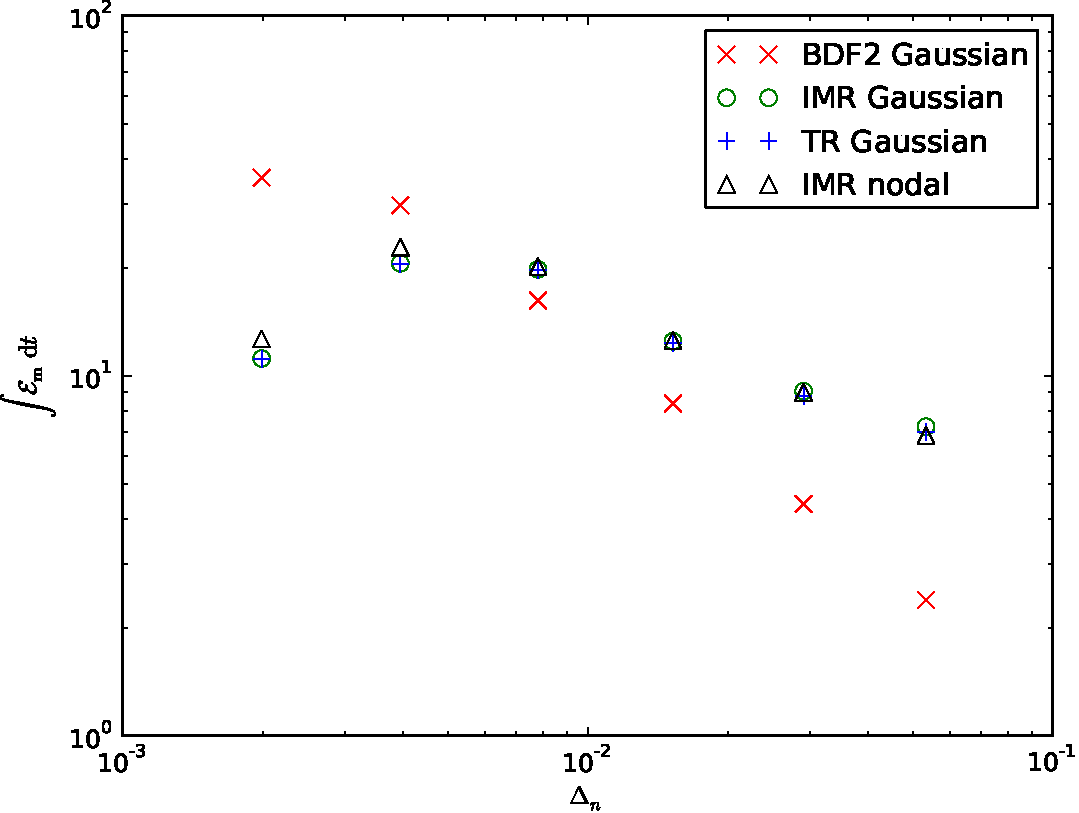
\includegraphics[width=0.9\textwidth]{plots/2d_wave_solution_convergence_long_time/errornormintegralvsfakemeanofdts.pdf}
  \caption{Convergence of $\intt{\errmpde}$, where $T=[0,5]$, for the 2D wave-like problem.
  }
  \label{fig:convergence-long-time-full-norm}
\end{figure}

To obtain more meaningful results we should use an alternative error norm which allows a better measure of the error even for approximate solutions which are out of phase with the exact solution.
One such error norm measures the deviation of $m_z$ from the exact value
\begin{equation}
  \errmz = \max_j \abs{m_{z,j,k} - m_z(t_n)}.
\end{equation}
Note that the exact value of $m_z$ is not a function of $\xv$ and so it is sufficient to take the maximum value.
This error norm measures the level of over/under damping caused by the approximation.

The convergence results for the time integral of the error norm $\errmz$ are shown in \cref{fig:convergence-long-time-mz-norm}.
We again see second order convergence behaviour for all methods.
The BDF2 method requires additional refinement to reach the asymptotic convergence behaviour, and has around an order of magnitude larger error than the other methods once convergence is reached.
Also note that there is no significant difference between IMR with nodal quadrature (which conserves $\abs{\mv}$) and IMR with Gaussian quadrature (in which $\mv$ is re-normalised), indicating that geometric integration offers no significant benefits in this case.
\begin{figure}
  \centering
  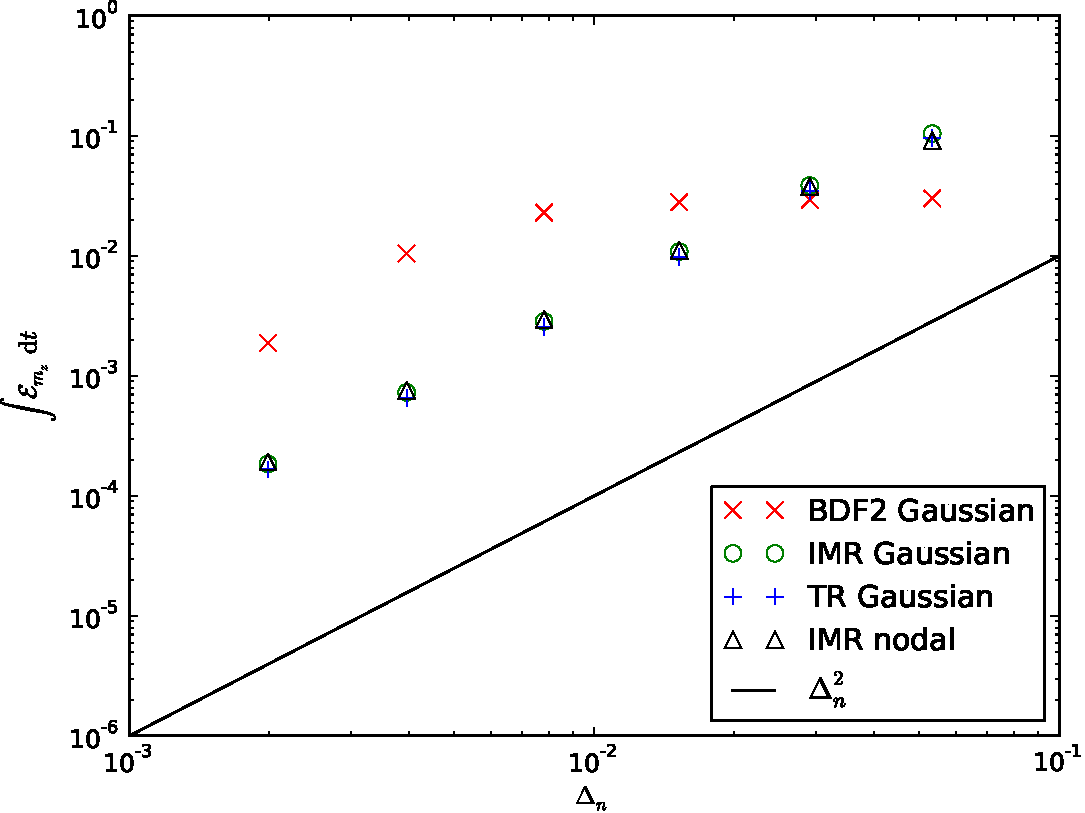
\includegraphics[width=0.9\textwidth]{plots/2d_wave_solution_convergence_long_time/auxerr1integralvsfakemeanofdts.pdf}
  \caption{Convergence of $\intt{\errmz}$, where $T=[0,5]$, for the 2D wave-like problem.
  }
  \label{fig:convergence-long-time-mz-norm}
\end{figure}

% % fix or remove:
% Our next error norm aims to measure the error in the frequency of the wave.
% It is defined as
% \begin{equation}
%   \begin{aligned}
%     \errphase &= \abs{\psi_{n,0} - \psi(t_n, 0)}, \\
%     &= ...,
%   \end{aligned}
% \end{equation}
% where $\psi(t_n, 0) = ...$ is the analytical phase of the wave at $\xv = \zerov$, and $\psi_{n,0}$ is the corresponding phase in approximate solution.
% The convergence results with this error norm are shown in \cref{fig:convergence-long-time-phase-norm}.
% Unfortunately it appears that this error norm is not much better than $\errmpde$ in terms of measuring the error outside of the asymptotic regime, and we can only draw the same conclusions as for that example.
% \begin{figure}
%   \centering
%   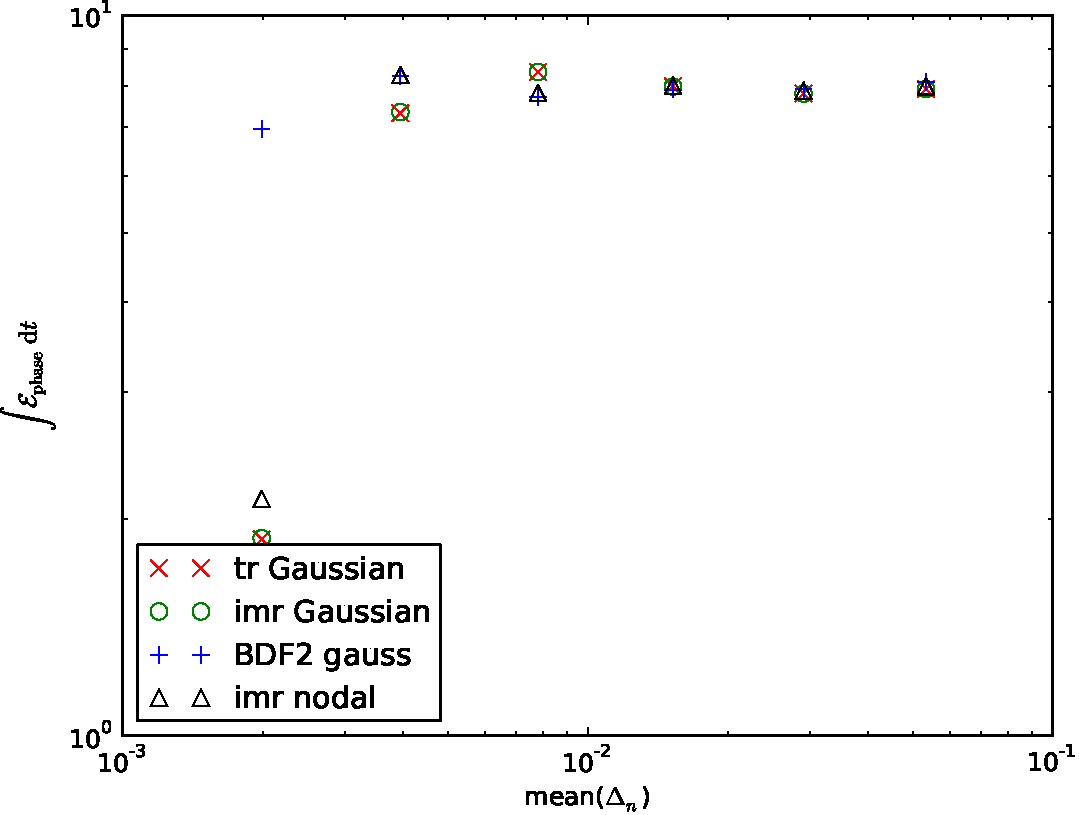
\includegraphics[width=0.9\textwidth]{plots/2d_wave_solution_convergence_long_time/auxerr0integralvsmeanofdts.pdf}
%   \caption{Convergence of $\intt{\errphase}$, where $T=[0,5]$, for the 2D wave-like problem.
%   }
%   \label{fig:convergence-long-time-phase-norm}
% \end{figure}



\subsection{Geometric integration properties}
\label{sec:2d-wave-results-cons-prop}

We now examine the error in nodal magnetisation length:
\begin{equation}
  \errml(t_n) = \max_j \abs{\abs{\mv_{j,n}} - 1},
  \label{eq:102}
\end{equation}
in the approximations generated by each of the time integration schemes (without re-normalisation).
\Cref{fig:mean-ml-error-2d} shows the evolution of $\errml$.
When using IMR with nodal quadrature the magnetisation length error remains extremely small, but for other methods the error rapidly grows to around $\order{10^{-4}}$ and seems to saturate at this level.
\begin{figure}
  \centering
  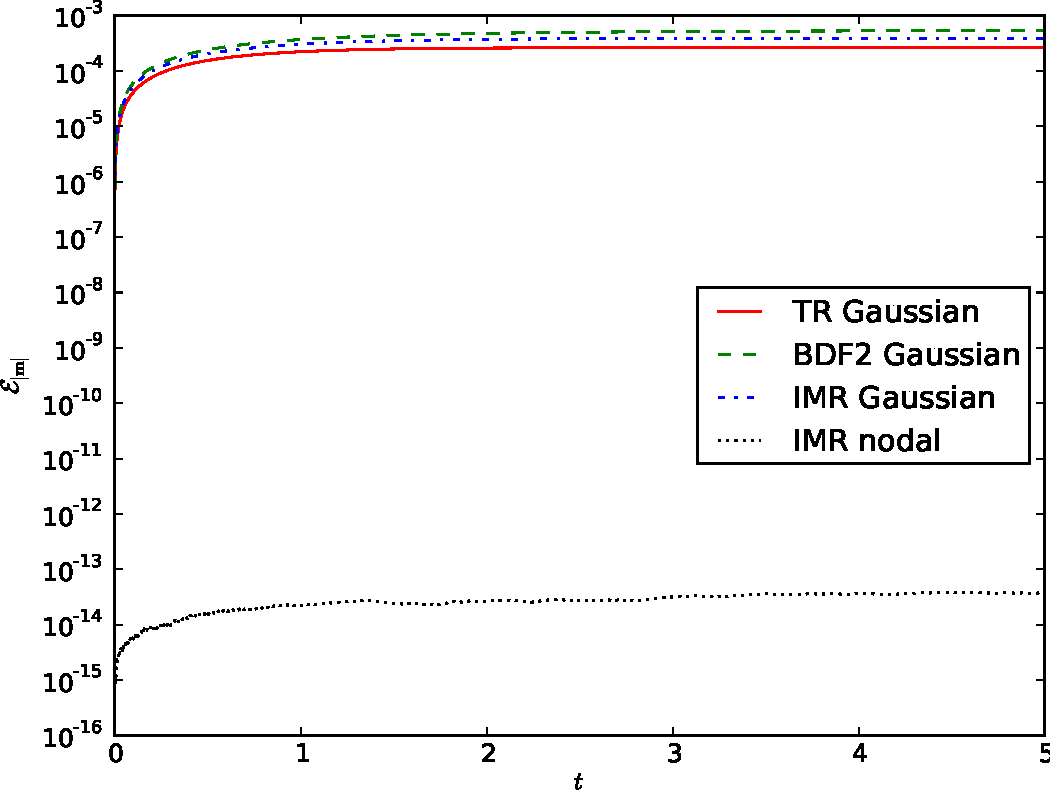
\includegraphics[width=0.8\textwidth]
  {plots/2d_wave_solution_m_length/mlengtherrormaxesvstimes.pdf}
  \caption{Evolution of $\errml$ with various time integrators and quadratures for the 2D wave-like problem.
  }
  \label{fig:mean-ml-error-2d}
\end{figure}

We next examine the energy conservation properties of the various schemes for the wave solution with $\dampc = 0$.
The only energy involved is the exchange energy, which can be calculated using \cref{eq:nd-e-ex}.
Note that these integrals can be evaluated exactly by either quadrature scheme because $\grad \mv$ is a constant inside each element.
The results are shown in \cref{fig:energy-error-2d}.
Interestingly we see that IMR with Gaussian quadrature and TR both conserve energy in a similar manner to IMR with nodal quadrature.
This is likely due to some special property of the exact solution, and does not appear to be the case in general (see \cref{sec:non-uniform-applied}).
\begin{figure}
  \centering
  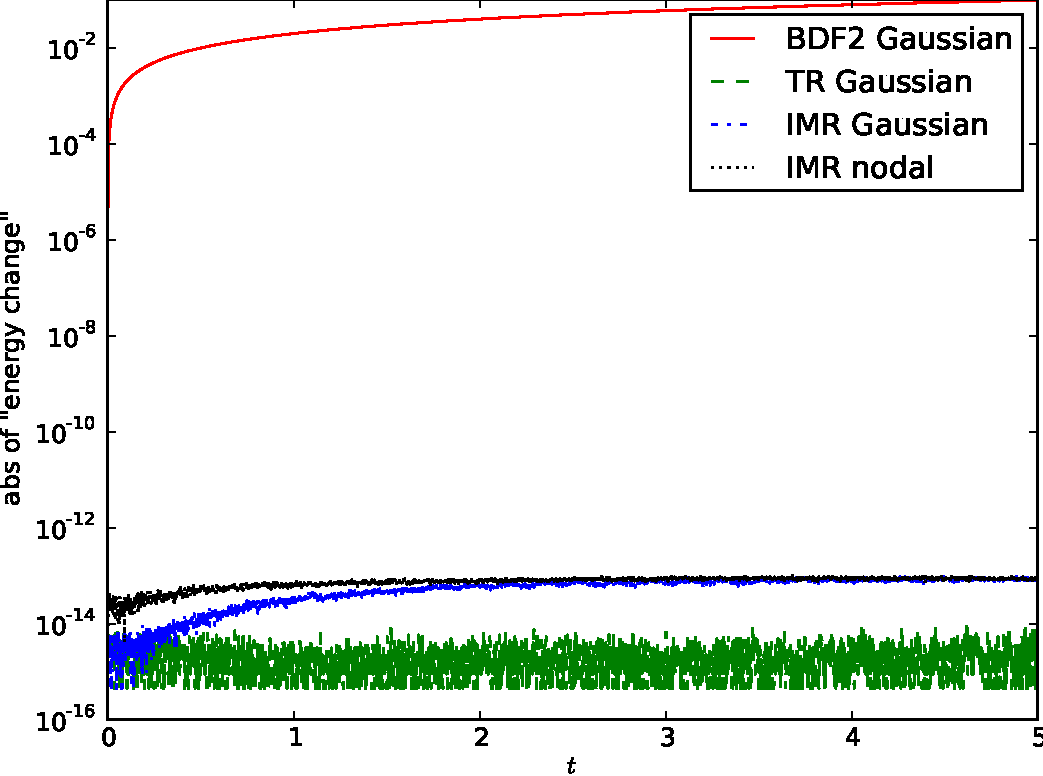
\includegraphics[width=0.8\textwidth]{plots/2d_wave_solution_energy/absofenergychangevstimes}
  \caption{Evolution of the error in energy with various time integration schemes and quadratures for the undamped 2D wave-like problem.
}
  \label{fig:energy-error-2d}
\end{figure}


\subsection{Effect of Newton tolerance}
\label{sec:effect-newt-toler-m-conservation}

As mentioned in \cref{sec:nodal-integration} we would expect to see some effect on the conservation properties when the accuracy of the linearisation method is varied.
In our implementation the Newton-Raphson method is used for linearisation, so the relevant measure of accuracy is the Newton tolerance, $\ntol$.

The obvious experiment to carry out would be to vary the Newton tolerance and examine how the error in $\abs{\mv}$ is affected.
However the Newton-Raphson method converges extremely quickly meaning that the final residual is often many orders of magnitude smaller than the tolerance, this would hide any correlation between the tolerance and the error.
Instead we plot the error against the \emph{actual} converged residual norm (specifically: the mean over all time steps of $\norm{\rv}_\infty$ after the Newton method has converged for that time step).
In order to generate a variety of converged residual norms we run the experiment with a range of parameters: $\ntol = 10^{-8}, 10^{-9}, 10^{-10}, 10^{-11}, 10^{-12}$; $\toltt = 10^{-3}, 10^{-4}, 10^{-5}$; $\dampc = 1, 0.001, 0$; and $h = 0.05, 0.025, 0.0125$.
We only integrate in time over the shorter interval $T = [0, 1]$ due to the volume of computations required.
The results are shown in \cref{fig:ml-error-2d-nodal-newton-tests}, there is a clear correlation between the magnitudes of the final residuals and the error in $\abs{\mv}$.
A similar result is seen in \cref{fig:energy-error-2d-nodal-newton-tests} for the energy conservation property when $\dampc = 0$.

\begin{figure}
  \centering
  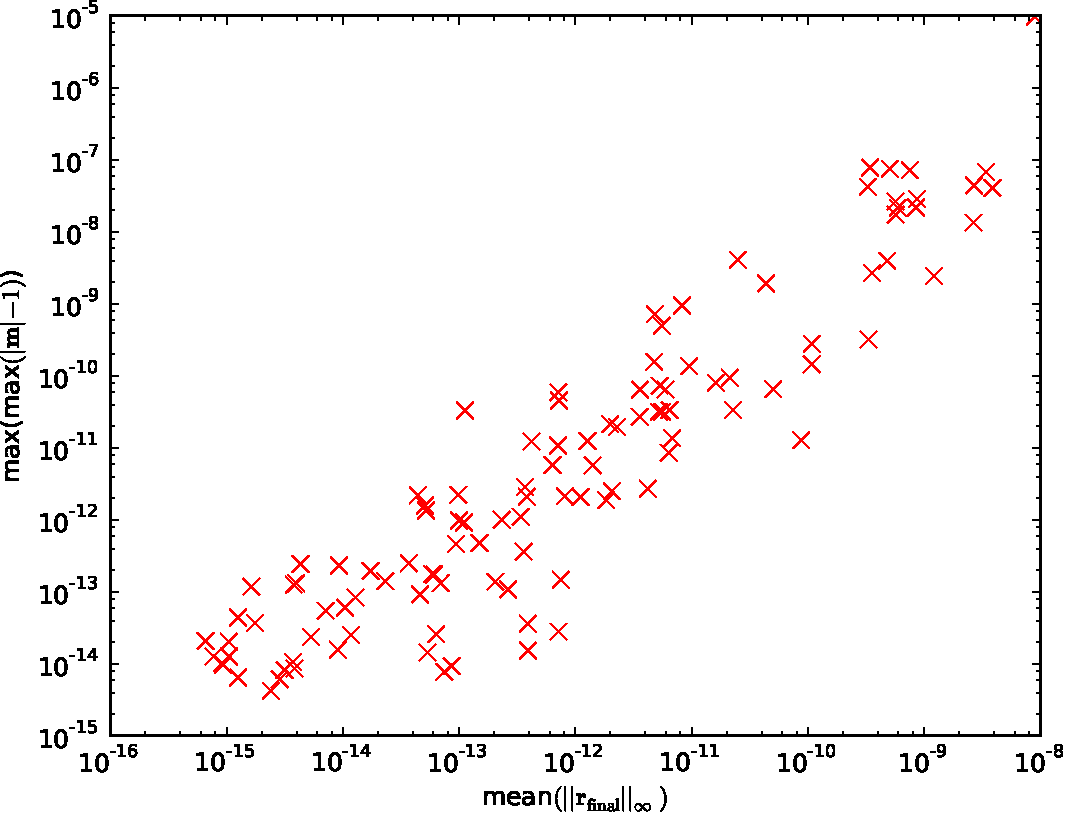
\includegraphics[width=0.8\textwidth]
{plots/2d_wave_solution_m_length_newton_res/maxofmlengtherrormaxesvsmeanminofnewtonresiduals.pdf}
  \caption{Correlation between maximum (over all nodes and all time steps) error of nodal magnetisation lengths and the mean (over time) of the converged Newton residual norm in the 2D wave-like problem solved using adaptive IMR and nodal quadrature.
  }
  \label{fig:ml-error-2d-nodal-newton-tests}
\end{figure}


\begin{figure}
  \centering
  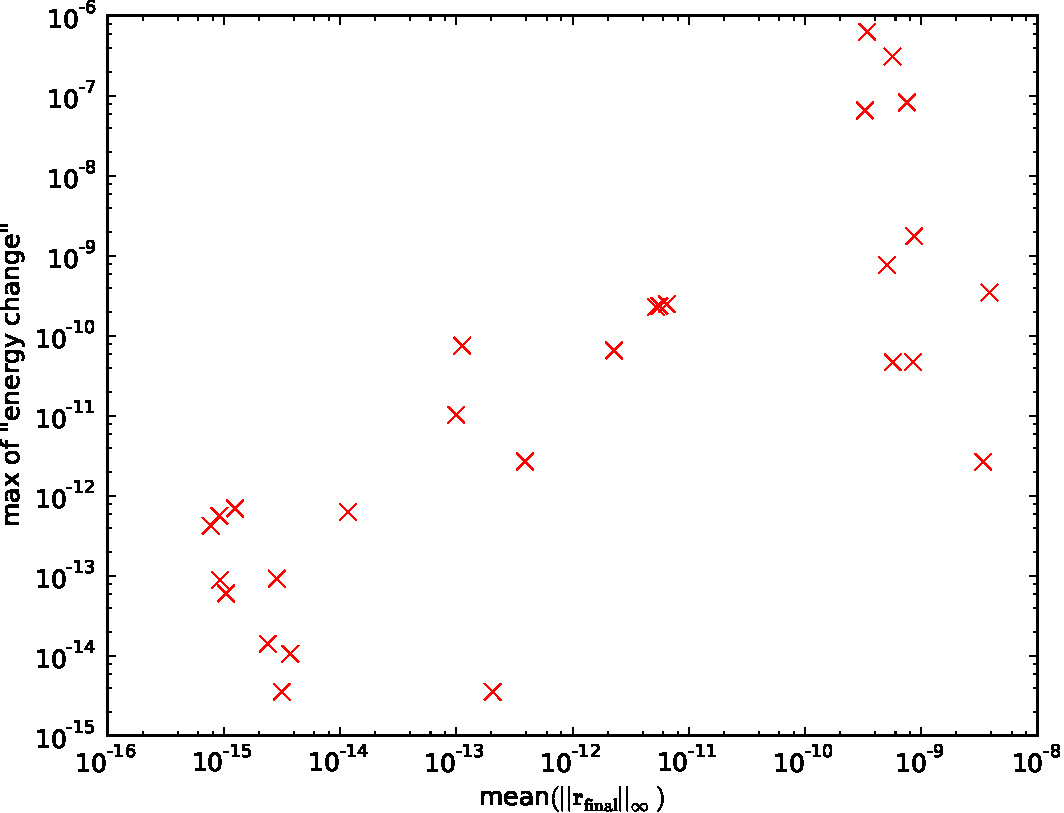
\includegraphics[width=0.8\textwidth]
  {plots/2d_wave_solution_energy_newton_res/maxofenergychangevsmeanminofnewtonresiduals.pdf}
  \caption{Correlation between the maximum (over time) of the error in energy and the mean (over time) of the converged Newton residual norm in the undamped 2D wave-like problem solved using adaptive IMR and nodal quadrature.
  }
  \label{fig:energy-error-2d-nodal-newton-tests}
\end{figure}



\subsection{Conclusions}

We have shown that the methods we tested have the expected convergence and time step selection properties.
We also observed that the asymptotic accuracy of the BDF2 method is lower than the TR or IMR methods by a moderately sized constant factor.

We have also shown that the geometric integration properties of IMR are preserved in a weak form FEM model with a nodal quadrature scheme.
As predicted in \cref{sec:nodal-integration} these properties are linked to the accuracy of the non-linear solver.

Additionally we observed unexpected geometric integration properties when IMR with Gaussian quadrature or TR are used.
It is expected that this is a consequence of the specific test problem rather than the methods themselves, and this conjecture will be tested in the next section.

Since all methods except for BDF2 showed some geometric integration properties the effect of such properties on the overall error cannot be analysed using this example.


\FloatBarrier
\section{An example with non-uniform applied field}
\label{sec:non-uniform-applied}

In \thisref{sec:non-uniform-applied} we construct a problem which is non-uniform in space without the involvement of the magnetostatic field by applying a non-uniform applied field.
This will allow us to examine whether the anomalous geometric integration properties observed in the previous section are related to the analytical solution.

This experiment also reveals some reduction in the effectiveness of the geometric integration on meshes of triangular elements.

\subsection{Problem definition}

We solve the LLG without magnetostatics on a two dimensional square domain $\magd = [0,5] \times [0,5]$ with Neumann boundary conditions.
The problem is integrated in time over $T = [0, 5]$.

We use a uniform initial condition $\mv = [1, 1, 0]/\sqrt{2}$ with a non-uniform applied field $\happ = [0, 0, h_z]$ where
\begin{equation}
  h_z =
  \begin{cases}
    1.1 (1 -  x) & x  < 1, \\
    0 & \mathrm{otherwise}.
  \end{cases}
\end{equation}
As before we use $\dampc = 0.01$ except for energy conservation experiments where we use $\dampc = 0$.

The dynamics occurring in this problem are quite simple: the magnetisation in the region of the domain $x<1$ moves towards $\mv = [0, 0, 1]$ by the applied field.
Exchange interactions force the rest of the domain to move towards the same field, albeit much more slowly, until eventually the entire domain is in a uniform state.

The implementation details of this example are exactly as described in \cref{sec:impl-deta}, except that we also use meshes of triangular elements.
The structure of the triangular element mesh is equivalent to the square element mesh except that the square elements are divided diagonally into two triangles.


\subsection{Geometric Integration properties}


The evolution of the magnetisation length for this experiment is shown in \cref{fig:nonuniform-h-ml-error}, we see that in this case only IMR with nodal quadrature conserves $\abs{\mv}$ as expected.
The same is true for the energy conservation with zero damping, as shown in \cref{fig:nonuniform-h-energy-error}.

\begin{figure}
  \centering
  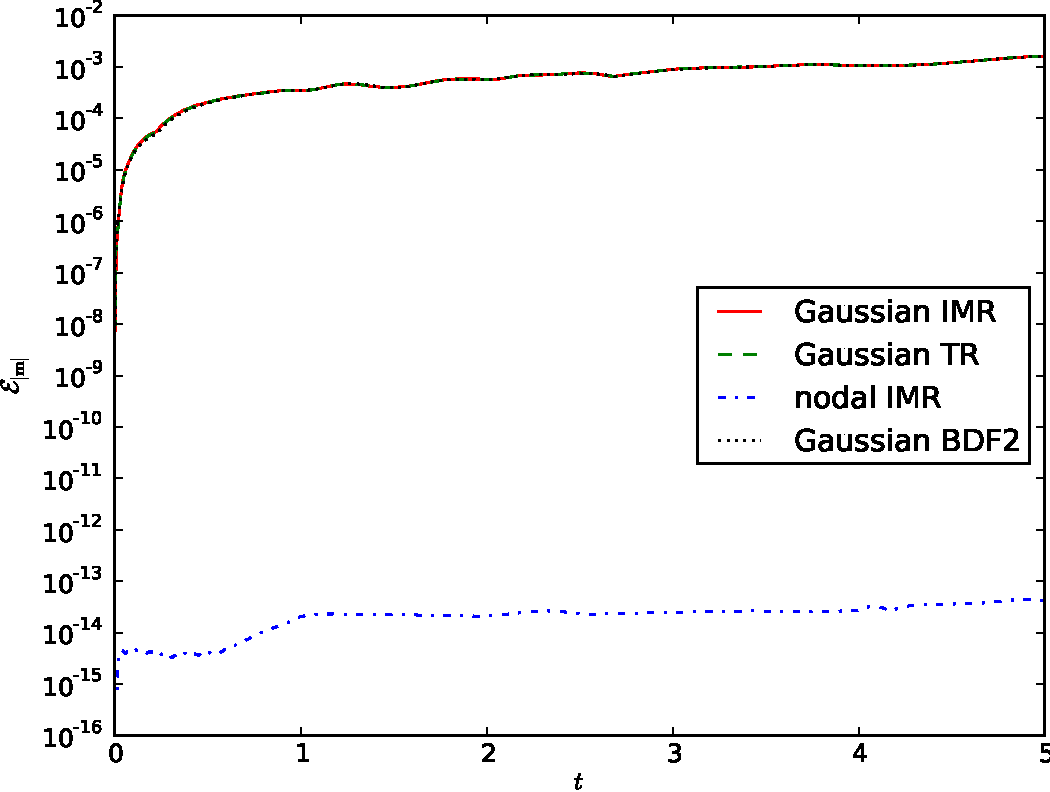
\includegraphics[width=0.8\textwidth]
  {plots/nonuniform-h-ml/mlengtherrormaxesvstimes.pdf}
  \caption{
    Evolution of $\errml$
    with various time integration schemes and quadratures
    for the 2D nonuniform field problem.
  }
  \label{fig:nonuniform-h-ml-error}
\end{figure}


\begin{figure}
  \centering
  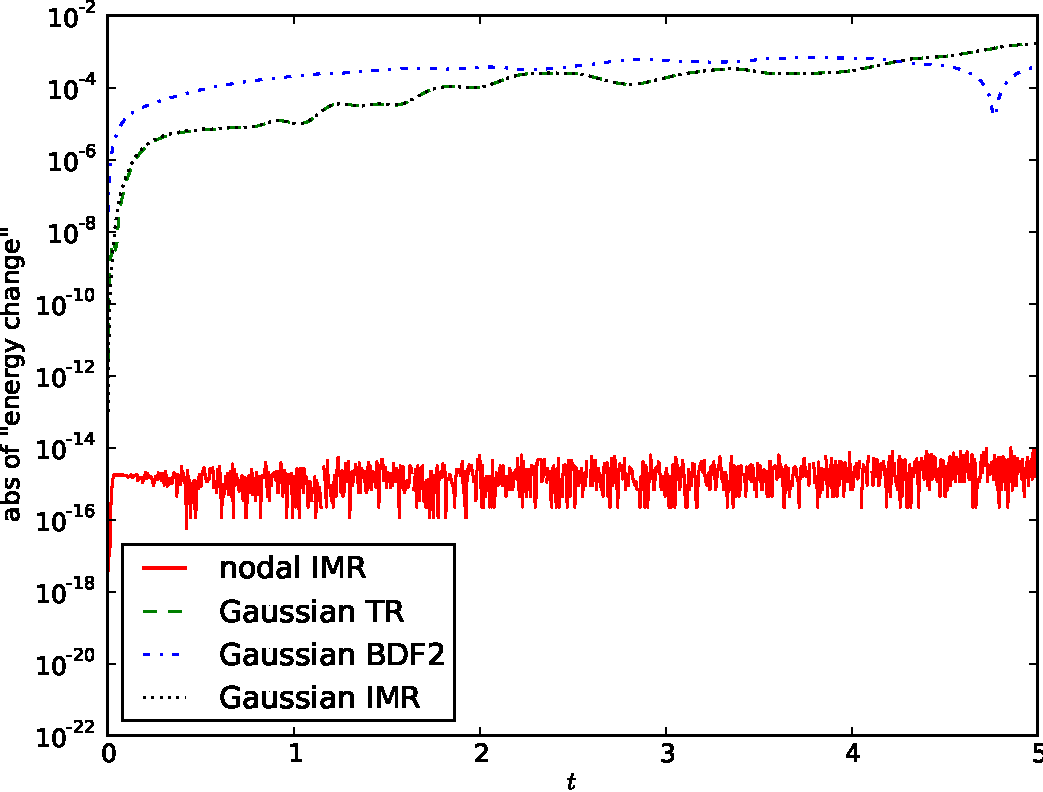
\includegraphics[width=0.8\textwidth]
  {plots/nonuniform-h-energy-change/absofenergychangevstimes.pdf}
  \caption{
    Evolution of the error in energy
    with various time integration schemes and quadratures
    for the undamped 2D nonuniform field problem.
  }
  \label{fig:nonuniform-h-energy-error}
\end{figure}


\subsection{Triangular meshes}
\label{sec:triangular-meshes}

Finally we show some results when a mesh of triangular elements is used.
The evolution of $\abs{\mv}$ is shown in \cref{fig:ml-error-triangle-mesh}.
We see that the error in $\abs{\mv}$ when using IMR with nodal quadrature is significantly larger on triangular elements than on square elements.
Similarly the error in the energy (with $\dampc = 0$) is significantly larger, as shown in \cref{fig:energy-error-triangle-mesh}.
Other experiments show this issue for a variety of other cases including 3D problems with tetrahedral elements, but not for the wave-like example above.

We do not have an explanation for this effect.
However it should be noted that the non-conservation effects are small enough that they would not be noticed if the numerical experiments were run with a loose non-linear solver tolerance, such as used in \eg \cite{Bartels2006}.

\begin{figure}
  \centering
  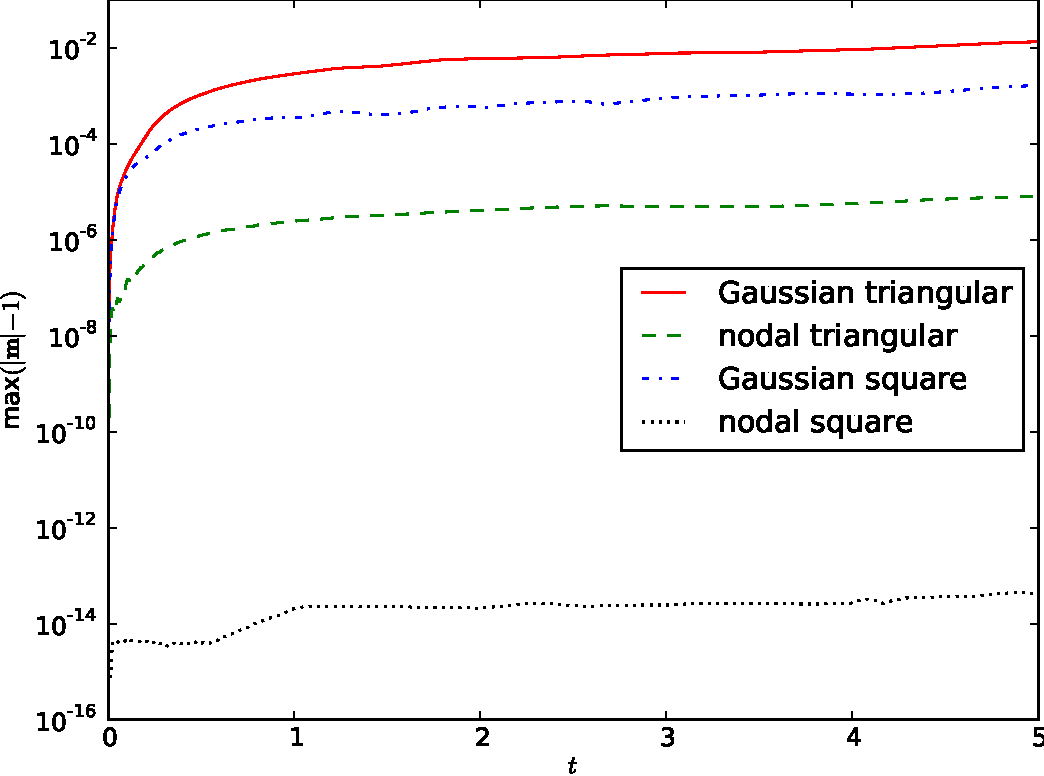
\includegraphics[width=0.8\textwidth]
  {plots/nonuniform-h-triangles-ml/mlengtherrormaxesvstimes.pdf}
  \caption{
    Evolution of $\errml$
    with IMR, both quadratures, and both element shapes
    for the 2D nonuniform field problem.
}
  \label{fig:ml-error-triangle-mesh}
\end{figure}

\begin{figure}
  \centering
  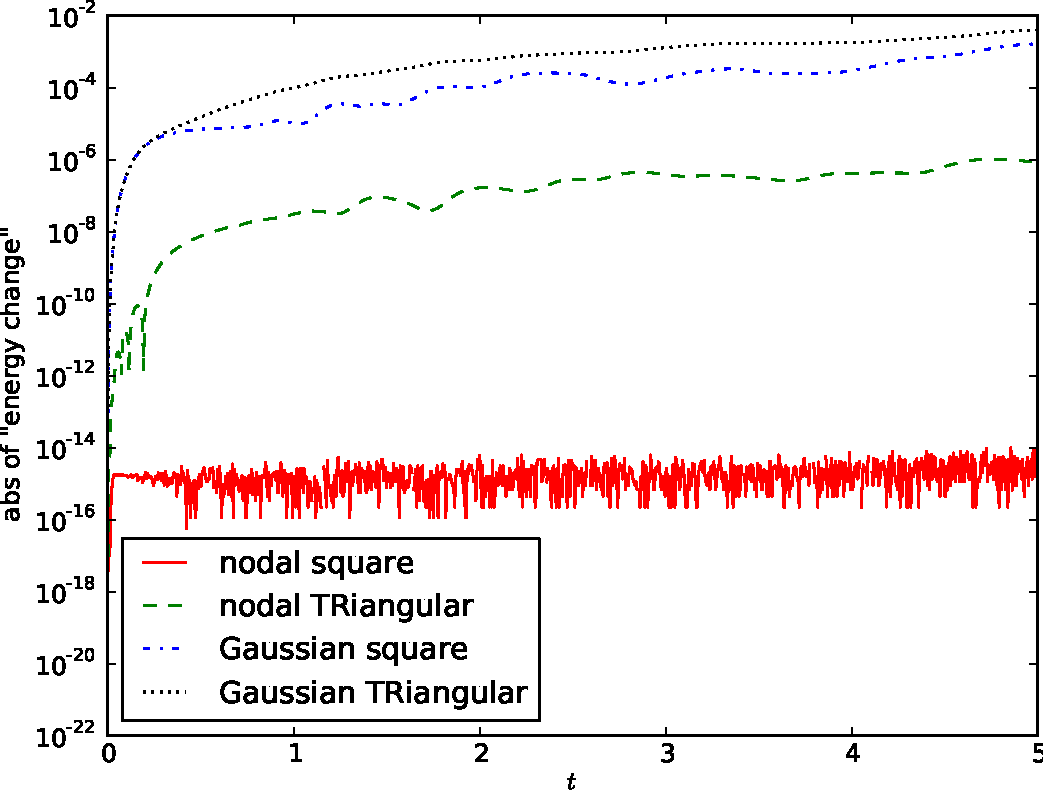
\includegraphics[width=0.8\textwidth]
  {plots/nonuniform-h-triangles-energy-error/absofenergychangevstimes.pdf}
  \caption{
    Evolution of the error in energy
    with various time integration schemes, quadratures, and element shapes
    for the undamped 2D nonuniform field problem.
  }
  \label{fig:energy-error-triangle-mesh}
\end{figure}

\subsection{Conclusions}

We have confirmed that the wave-like example is in some sense ``too easy'' and does not provide a rigorous test of geometric integration properties: IMR with Gaussian quadrature and TR do not conserve energy or $\abs{\mv}$ in general.

We have also shown an example problem where our implementation of IMR with nodal quadrature unexpectedly gives significantly worse conservation of energy and $\abs{\mv}$ when used with a mesh of triangular elements, as compared to square elements.


% Don't allow floats from last section into this one
\FloatBarrier
\section{The \mumag standard problem \#4}
\label{sec:mumag-stand-probl}

The \mumag standard problem \#4 \cite{mumag-website} is the benchmark problem most widely used to test implementations of dynamic micromagnetic models.
It involves modelling the reversal of an extremely thin cuboid film of permalloy-like material under two different applied fields.
Unfortunately FEM/BEM magnetostatic calcultations are ill-suited to thin film problems: the dense BEM matrix size is proportional to the number of nodes on the boundary and in a thin film every single node is on the boundary.
Additionally the key benefit of FEM/BEM (accurate resolution of complex geometries) is not required since the film is a simple cuboid.
However, since there are no other widely studied test problems and there are no problems with non-trivial magnetostatic and exchange effects for which an analytical solution is known, we use the standard problem to verify our implementation.


\subsection{Problem specification}

The magnetic domain is a sheet of magnetic material $500 \times 125 \times 3$nm with material parameters
\begin{equation}
  \begin{aligned}
    A &= 1.3\E{-11} \text{J/m}, \\
    M_s &= 8.0\E{5} \text{A/m}, \\
    \Kone &= 0.0, \\
    \gymagc &= 2.211 \E{5} \text{m/As}, \\
    \dampc &= 0.02.
  \end{aligned}
\end{equation}
The simulation is run with two different applied fields:
\begin{equation}
  \begin{aligned}
    \mu_0 \happ_{,1} = [-24.6, 4.3, 0.0] \;\text{mT}, \\
    \mu_0 \happ_{,2} = [-35.5, -6.3, 0.0] \;\text{mT}, \\
  \end{aligned}
  \label{eq:mumag-h-app}
\end{equation}
where $\mu_0 = 4\pi\times10^{-7}$.
The initial condition is the S-state given by slowly relaxing the magnetisation from the state created by a saturating field in the $[1,1,1]$ direction.

These magnetic parameters result in a magnetostatic exchange length (and unit length in our simulations) of
\begin{equation}
  l_{\text{ex}} = \sqrt{\frac{2A}{\mu_0 M_s^2}} = 5.6858\text{nm},
\end{equation}
hence the normalised dimensions are approximately $87.94 \times 21.98 \times 0.53$.
Our unit time is
\begin{equation}
  t_{\text{unit}} = \frac{1}{\gymagc M_s} = 5.653\text{ps}.
\end{equation}


\subsection{Implementation details}

We use the FEM to spatially discretise the LLG equation and the Newton-Raphson method to solve the resulting non-linear systems as described in \cref{sec:galerk-meth-llg}.
The hybrid FEM/BEM method, described in \cref{sec:hybr-finit-elem}, is used for magnetostatic calculations.
For the coupling of the LLG equation with the magnetostatic calculations we use both the monolithic and semi-implicit methods discussed in \cref{sec:solution-strategies}.
The solution of the monolithic linear system is done using the fully iterative preconditioner $\inexact{\precc}$, it turns out that for thin film problems the ILU(1) approximation to the LLG block, $\Fm$, is effective.
The decoupled systems resulting from the semi-implicit method are solved using the methods described in \cref{sec:llg-only-system}.
Both methods use the parameters described in \cref{sec:linear-systems-probl-spec}.

The TR, BDF2 and IMR adaptive time integration schemes (see \cref{sec:adapt-impl-midp,sec:aimr-implementation}) are used with both the Gaussian and nodal quadrature schemes.
For those schemes which do not naturally conserve $\abs{\mv}$ both normalised and re-normalised versions are tested.

As previously mentioned, the adaptive IMR requires an explicit time step for the estimation of the error.
This is implemented as described in \cref{sec:impl-deta}.
No coupling with the FEM/BEM calculations is required for this explicit step because only the value of the magnetostatic potential at the $n$-th time step is required (which is already known from the IMR calculations).

A structured mesh consisting of cuboid elements is used due to the simple geometry of the problem and the fact that we have observed issues with geometric integration on tetrahedral elements (see \cref{sec:triangular-meshes}).
In the $z$ direction (out of the thin film plane) a single layer of elements is used at all refinements.
This is a standard approach, and is expected to give acceptable resolution because the exchange length of the material (the length scale over which the magnetisation can vary strongly) is around twice the thickness.
The number of elements along the $x$ and $y$ axes, denoted $n_x$ and $n_y$, is varied but the ratio is fixed at $n_x = (500/125) n_y$ so that the element edge lengths in each direction are identical.
We use $n_x=75,100,125$, which gives edge lengths of 1.17, 0.89 and 0.70 exchange lengths respectively.

The Newton tolerance is set to $\ntol = 10^{-11}$, the adaptive integrator tolerance is $\toltt = 10^{-5}$ and the initial time step is $\dtx{0} = 10^{-4}$.
% We cap the time step at $\dtx{\text{max}} = 4.5$ to avoid issues with linear and solver converge at extremely large time steps.


To generate the initial S-state we run the simulation for 300 time units starting from the state $\mv=[1,1,1]$ with $\dampc = 1.0$ and the applied field
\begin{equation}
  \happ_i(t) =
  \begin{cases}
    10 (1- \frac{t}{100}) & t < 100, \\
    0 & t \geq 100.
  \end{cases}
\end{equation}
The time integrator history data is then set such that it has been in this state forever and the time step sizes are set to the initial value.
The relevant applied field as specified in the problem is set and the simulation is continued.
The initial condition is always generated using the same numerical methods as are used in the dynamic part of the simulation.

Note that with $\dampc = 1$ the time scale for the magnetisation to relax is much shorter than with $\dampc \sim 0.01$.
Hence the simulated time allowed for relaxation to the initial condition is sufficiently long to be considered ``slow'' despite the fact that it is much shorter than the simulated time for the dynamics calculations.


We compare our results against those submitted to the \mumag website by d'Aquino \etal \cite{mumag-website}.
These results were generated by a fixed time step IMR scheme with a finite difference spatial discretisation monolithically coupled to a fast Fourier transform method for magnetostatic calculations \cite{DAquino2005}.



\subsection{General results}

For this problem we find that without either re-normalisation or geometric integration the time steps selected by the adaptive algorithms become unacceptably small (\ie the error becomes large).
Hence these cases were not run until completion and are not included in the results.

In \cref{fig:intial-mumag4} we show the initial S-state, as generated by IMR with nodal quadrature.
\begin{figure}
  \centering
  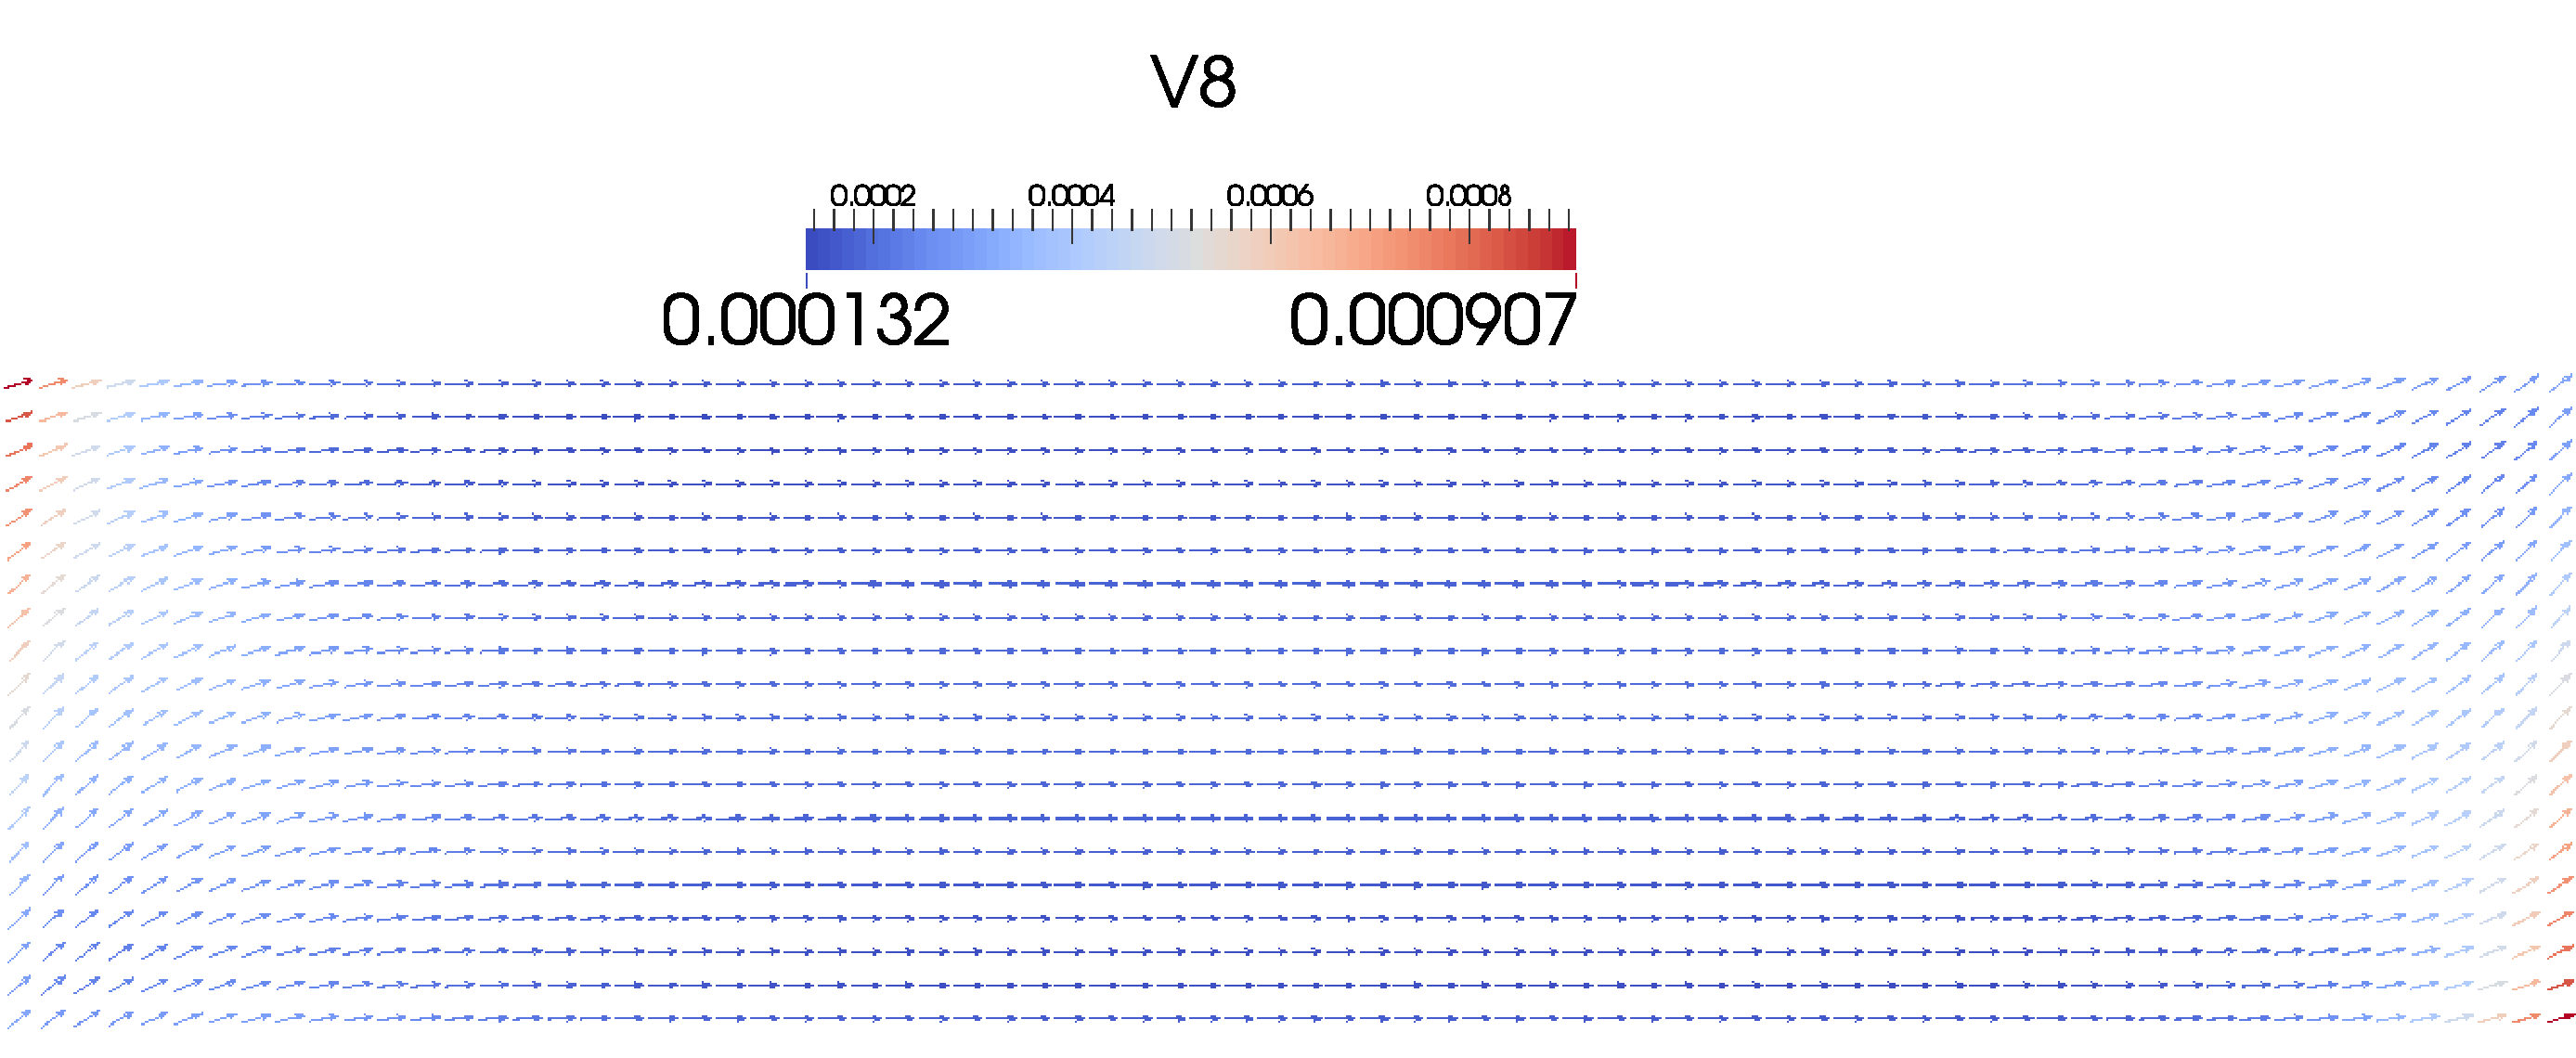
\includegraphics[width=0.8\textwidth]{images/mumag4-s-state.pdf}
  \caption{Initial S-state as generated by adaptive IMR with nodal quadrature and $n_x=75$ nodes along the $x$ direction.
    Colour indicates the $z$ (out of plane) component of magnetisation.
  }
  \label{fig:intial-mumag4}
\end{figure}

Next we show the mean magnetisation for the two fields from \cref{eq:mumag-h-app} in \cref{fig:nmag-comparison-mumag4-field1,fig:nmag-comparison-mumag4-field2} respectively.
Our results with smaller numbers of nodes, other time integration schemes, and smaller adaptive time integrator tolerance agree well with the results shown in \cref{fig:nmag-comparison-mumag4-field1,fig:nmag-comparison-mumag4-field2}.

The results agree reasonably well with the results obtained by d'Aquino except around $t=100$ when field 2 is used (\cref{fig:nmag-comparison-mumag4-field2}).
We have also tested the behaviour when using IMR with fixed time steps or alternative methods for generating the initial S-state but these have no effect on the discrepancy.
However, it is worth noting that all of the submitted solutions on the \mumag website \cite{mumag-website} behave differently for this part of the problem!
The issues may be due to corner singularities in the magnetostatic field and, if so, could be resolved by the use of higher order solution and test basis functions for the magnetostatic potential \cite{Schrefl1997}.


The same plots show the time step selection behaviour.
During relaxation (negative time in the figures) the time step has a large value initially, which decreases as the field decreases and the relaxation takes place, then become very large once the field reaches zero.
During the dynamics (positive time in the figures): a reasonable large time step is selected initially.
It then decreases around the time of the peak in $\mv$ and steadily increases as the oscillations are damped out.
The behaviour observed for the second field is essentially the same.

\begin{figure}
  \centering
  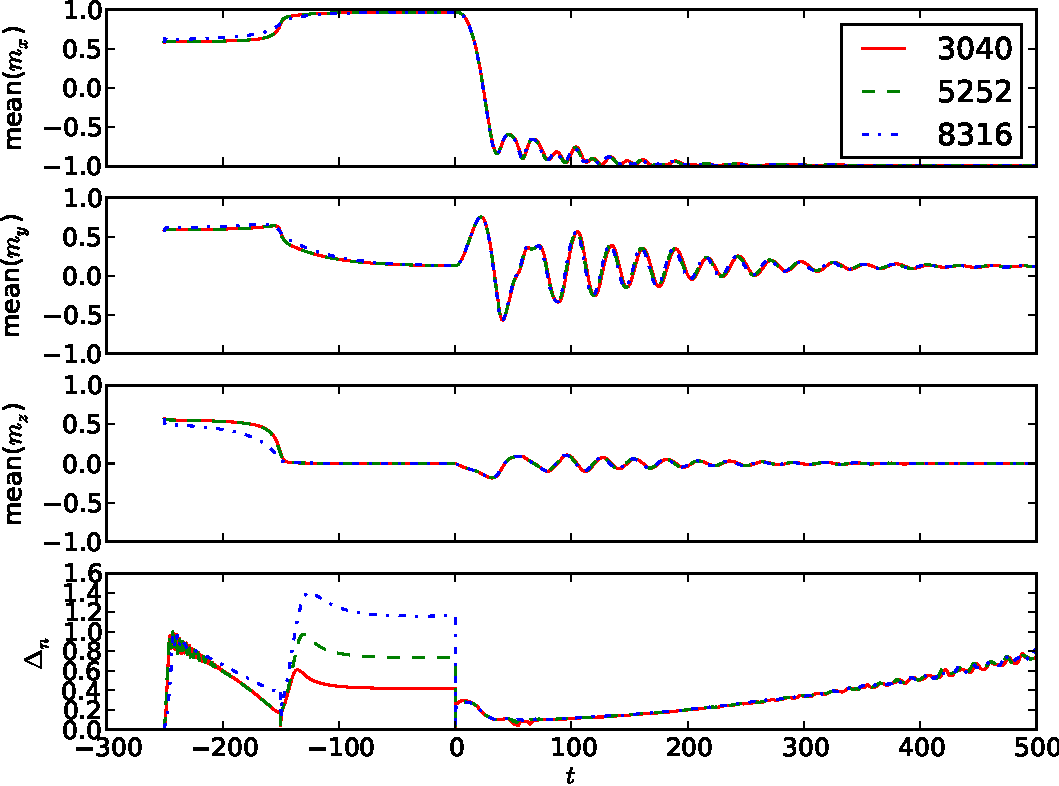
\includegraphics[width=0.8\textwidth]{plots/mumag4_convergence/mumag4_field1-meanmxsvs-meanmysvs-meanmzsvs-dtsvstimes.pdf}
  \caption{
    Evolution of the mean magnetisation for the \mumag problem \#4 with field 1 using monolithic IMR with nodal quadrature.
    For comparison we also show the results submitted to the \mumag website by d'Aquino \etal \cite{mumag-website}.
}
  \label{fig:nmag-comparison-mumag4-field1}
\end{figure}

\begin{figure}
  \centering
  \includegraphics[width=0.8\textwidth]{plots/mumag4_convergence/mumag4_field2-meanmxsvs-meanmysvs-meanmzsvs-dtsvstimes.pdf}
  \caption{
    Evolution of the mean magnetisation for the \mumag problem \#4 with field 2 using monolithic IMR with nodal quadrature.
    For comparison we also show the results submitted to the \mumag website by d'Aquino \etal \cite{mumag-website}.
  }
  \label{fig:nmag-comparison-mumag4-field2}
\end{figure}


%
% Also the state of the system at the time when $m_x$ crosses zero for field 2 is shown in \cref{fig:mumag4-spatial-x-crossing-0}.

% \begin{figure}
%   \centering
%   \includegraphics[width=0.8\textwidth]{images/placeholder}
%   \caption{The state of the system at the time when $m_x$ crosses zero}
%   \label{fig:mumag4-spatial-x-crossing-0}
% \end{figure}


We show a comparison of the solution generated using IMR with nodal quadrature and monolithic or decoupled approach in \cref{fig:mumag4-implicit-decoupled}.
The dynamics are very similar, but the monolithic method is able to take larger time steps and has less noise in the size step during the initial relaxation.
\begin{figure}
  \centering
  \includegraphics[width=0.8\textwidth]
  {plots/monolithic_vs_decoupled/meanmxsvs-meanmysvs-meanmzsvs-dtsvstimes.pdf}
  \caption{
    Evolution of the mean magnetisation for the \mumag problem \#4 with field 2 using IMR with nodal quadrature and monolithic (implicit) or semi-implicit (decoupled) coupling to the magnetostatics problem.
  }
  \label{fig:mumag4-implicit-decoupled}
\end{figure}

\subsection{Geometric integration properties}

The evolution of the maximum nodal error in the magnetisation length for the decoupled and implicit methods is shown in \cref{fig:imr-conservation}.
As expected both coupling approaches conserve $\abs{\mv}$ to around the Newton tolerance.
\begin{figure}
  \centering
  \includegraphics[width=0.8\textwidth]{plots/mumag4_ml/mlengtherrormaxesvstimes.pdf}
  \caption{
    Evolution of $\errml$
    with IMR, nodal quadrature and both coupling strategies
    for the \mumag problem \#4 with field 2.
  }
  \label{fig:imr-conservation}
\end{figure}


The evolution of the energy of the system when $\dampc = 0$ is shown in \cref{fig:energy-conservation}.
It can be seen that neither the monolithic or decoupled methods give the desired conservation behaviour.
From various other experiments we have drawn the conclusion that this occurs when the magnetostatic calculations are introduced.
\begin{figure}
  \centering
  \includegraphics[width=0.8\textwidth]
  {plots/sq_mumag4_energy_conservation/absofenergychangevstimes.pdf}
  \caption{
    Evolution of the error in energy
    with various time integration schemes, quadratures, and coupling strategies
    for the undamped \mumag problem \#4 with field 2.
    Results for other combinations of methods are very similar.
  }
  \label{fig:energy-conservation}
\end{figure}

We believe that the lack of energy conservation is due to the asymmetry of the discrete BEM operator.
This asymmetry be expected to cause issues with energy conservation because the symmetry property \cref{eqn:imr-linop} no longer holds, and the energy property \cref{eq:orth-energy} cannot be derived.
Standard collocation based discretisation approaches, as used in our discretisation of the BEM operator, do not preserve the symmetry of the underlying operators.
A symmetric discrete BEM operator could be obtained by applying a \emph{symmetric Galerkin} BEM discretisation \cite{Bonnet2003} \cite[75]{Wrobel2002} to the formulation discussed in \cref{sec:hybr-finit-elem}.
Alternatively a standard Galerkin BEM discretisation combined with the single-layer-potential formulation described by Garc\'{i}a-Cervera and Roma \cite{Garcia-Cervera2006} \cite[19]{Knittel2011} would result in a symmetric discrete operator without the requirement to evaluate hyper-singular integrals.



\subsection{Effectiveness of the linear and non-linear solver}
\label{sec:effect-line-non}

In this section we examine the effectiveness of the iterative linear and non-linear solvers for the monolithic method introduced in \cref{sec:fully-implicit-bem} as applied to the \mumag standard problem \#4.

The mean number of iterations required for the convergence of the linear solver against the number of nodes in the problem is shown in \cref{fig:mumag4-solver-iterations}.
Note that while the iteration count increases with the number of nodes, $\Nn$, it remains reasonable for the problem sizes required for good accuracy in this example.
The time taken to set up the preconditioner is displayed in \cref{fig:mumag4-solver-time}.
Again it grows with the number of nodes but remains reasonable for all cases shown here.
Also note that with nodal quadrature the preconditioner is cheaper to set up but less effective.
To counteract this effect a higher level of ILU fill-in could be used with nodal quadrature.

\begin{figure}
  \centering
  \includegraphics[width=0.8\textwidth]
  {plots/mumag4_monolithic_its/meanofnsolveritersvsinitialnnode.pdf}
  \caption{
    GMRES iterations to converge against problem size for the monolithic system using the inexact preconditioner $\inexact{\precc}$ with the various time integration schemes, quadratures, and applied fields for the \mumag problem \#4 (including the calculation of the relaxed initial condition).
}
  \label{fig:mumag4-solver-iterations}
\end{figure}

\begin{figure}
  \centering
  \includegraphics[width=0.8\textwidth]
  {plots/mumag4_monolithic_its/meanofpreconditionersetuptimesvsinitialnnode.pdf}
  \caption{
    Time in seconds to set up the inexact preconditioner $\inexact{\precc}$
    against problem size for the monolithic system using the inexact preconditioner $\inexact{\precc}$
    with the various time integration schemes, quadratures, and applied fields
    for the \mumag problem \#4 (including the calculation of the relaxed initial condition).
  }
  \label{fig:mumag4-solver-time}
\end{figure}


Next we look at the number of iterations of the Newton-Raphson method required to solve the monolithically coupled non-linear system.
The mean number of iterations required for convergence is consistently just over 2 (and always less than 3) despite the extremely tight tolerance and the very large time steps (during the calculation of the initial condition and towards the end of the simulation).
In particular, we note that the number of iterations required is significantly lower than the $\sim 14$ quasi-Newton iterations required for the monolithic method used in \cite{DAquino2005}.
The various other example problems covered in this chapter required similar numbers of Newton-Raphson iterations.

\begin{figure}
  \centering
  \includegraphics[width=0.8\textwidth]
  {plots/mumag4_monolithic_its/meanofnnewtonitersvsinitialnnode.pdf}
  \caption{Newton-Raphson iterations to converge against problem size
    for the monolithic system with the various time integration schemes, quadratures, and applied fields for the \mumag problem \#4 (including the calculation of the relaxed initial condition).}
  \label{fig:mumag4-newton-iters}
\end{figure}


We do not explore the total solve times of the various methods for this example.
The solve times are dominated by the calculations involving the BEM matrix due to the fact that we have not used a hierarchical matrix representation of the dense block and the extremely large number of boundary nodes.
Hence any timing results would be meaningless for practical problems in which the FEM/BEM method is appropriate.


\subsection{Conclusions}

Our methods give results for the \mumag problem \#4 which converge well and match up reasonably with the benchmark results of other models.

We observe the expected conservation of magnetisation length with IMR and nodal quadrature.
However, we do not observe the expected conservation of energy.
Asymmetry of the BEM part of the problem, and could be resolved by the use of alternative formulations and/or discretisation approaches.

Finally we have shown that, aside from issues with the lack of a hierarchical matrix implementation for rectangular boundary elements, we can efficiently solve the monolithic non-linear problem resulting from coupling the LLG with FEM/BEM magnetostatics calculations.
Application of Newton-Raphson method results in around 2.2 Newton iterations per non-linear solve on average.
The use of GMRES preconditioned by $\inexact{\precc}$ from \cref{sec:bem-solver-strategies} results in around 15 Krylov iterations per linear solve, with a reasonable preconditioner setup time.



\section{Conclusions}

In this chapter we have demonstrated the effectiveness of the methods described and developed throughout this thesis on micromagnetic problems with spatial variations.

We observed that our adaptive IMR algorithm selects appropriate time steps even for complex problems involving exchange and magnetostatics.
We have shown that IMR with nodal quadrature retains its magnetisation length conservation property on a number of problems, but also that it is less effective on certain meshes of triangular elements.
Similarly IMR (with nodal quadrature) provides energy conservation for problems without FEM/BEM magnetostatics, but that the energy conservation fails when collocation FEM/BEM magnetostatics calculations are included.
This issue is likely due to the asymmetry of the discrete BEM operator and could be avoided by using an alternative formulation and/or discretisation of the BEM problem.

Our methods converge exactly as expected to an exact solution of the LLG with exchange effective field.
Their accuracy on the \mumag standard problem \#4 with the first applied field also appears to be very good.
For the second field the results agree well with a finite difference based method using a similar time integration scheme only up to $t=100$, but all of the solutions submitted to the \mumag website disagree around this time.


%%% Local Variables:
%%% mode: latex
%%% TeX-master: "main"
%%% End:


\chapter{Conclusions and future work}
\chaptermark{Conclusions}

\section{Conclusions}

In this thesis we have introduced a complete numerical method for the solution of dynamic micromagnetic problems using the finite element method with the Newton-Raphson linearisation, a variety of implicit time integration schemes, hybrid FEM/BEM magnetostatics calculations, and efficient iterative linear solvers.
The methods have been validated against an analytical solution for a problem without magnetostatics and against the \mumag standard problem \#4 with magnetostatics.

In \cref{sec:adaptive-imr} we have demonstrated a novel and widely applicable adaptive time step selection algorithm for the implicit midpoint rule.
We have also shown that the time step selection works well for a wide variety of ODE test cases, as well as for a number of PDE test cases using the LLG equation.
Additionally we have shown that the geometrical integration properties of the constant time step IMR extend to the adaptive time step version.

In \cref{sec:solut-coupl-syst,sec:numer-exper-fem-bem-systems,sec:mumag-stand-probl} we introduced and tested efficient, robust and scalable solution methods for the monolithically coupled LLG-FEM/BEM magnetostatics problem provided that a good preconditioner for the LLG sub-problem is available.
Such monolithic couplings are required to obtain the energy property of the implicit midpoint rule and may offer advantages in stochastic integration methods.

In \cref{sec:imr-ode-llg-numer-exper,sec:numer-exper} we studied the performance of common implicit time integration schemes on some micromagnetic problems with exact solutions.
We found that the overall accuracy of the BDF2 scheme is always poor compared to the TR and IMR schemes, this is probably due to a combination of the larger local truncation error and the spurious numerical damping of BDF2.
% Unfortunately we were unable to analyse the effect of geometric integration on the error accumulation due to the fact that TR also displays some geometrical integration properties for these simple examples.

Finally in \cref{cha:stiffn-llg-equat} we studied the effect of spatial discretisation on the relative performance of implicit and explicit time integration schemes (stiffness).
We found that stiffness in micromagnetics can arise from the spatial discretisation alone, and that the stiffness increases as the element size is decreased, as expected from standard PDE theory.
We also found that the introduction of FEM/BEM magnetostatics calculations increases the stiffness.



\section{Future work}
\label{sec:future-work}


In the course of our numerical experiments we uncovered some issues with the geometrical integration properties of our complete model.
Firstly we found that the conservation properties of IMR with FEM and nodal quadrature was much less effective when applied to meshes of triangular elements, at least in our implementation.
This effect is fairly small and is not contradicted by any numerical results in the literature that we are aware of due to the common use of comparatively loose linearisation tolerances.
An alternative implementation of IMR with FEM and nodal quadrature should be used with a tight linearisation tolerance in order to find out if this effect is an artefact of our implementation or a real issue.

Secondly, we found that when FEM/BEM magnetostatics calculations discretised by a collocation based approach were included the energy conservation property of IMR was lost.
This is probably due to the asymmetry of the discrete BEM operator, which could be corrected by the use of alternative formulations of the method.
In particular the use of the Garc\'{i}a-Cervera-Roma formulation \cite{Garcia-Cervera2006} \cite[19]{Knittel2011} with a Galerkin discretisation approach \cite[75]{Wrobel2002} should resolve this issue.

Once these issues have been corrected the relative performance of schemes with geometric integration properties, in terms of the accumulation of the temporal error, should be evaluated for realistic problems.

In the area of linear solvers a general, efficient, robust and scalable preconditioner for the Newton-Raphson linearised LLG equation is still required.
One approach to the construction of such a preconditioner could be to exploit the block structure of the Jacobian matrix and to use multigrid-based methods to approximate the Laplacian-like skew-symmetric off-diagonal blocks resulting from the exchange effective field.
A less general approach for the case of granular or patterned media could be the use of a domain decomposition preconditioner.
In such a method the small matrix block associated with each grain/island would be inverted by a direct solver and the combination used as a block diagonal preconditioner.
Due to the weak coupling between grains/islands this would provide a good approximation for the inverse of the entire LLG block.
With either of these enhanced LLG preconditioners the effectiveness of the preconditioner discussed in \cref{sec:solution-strategies} on extremely large problems could be investigated.


In the time integration of the stochastic LLG only a few time integration schemes are known to converge to the correct solution, one of which is the implicit midpoint rule \cite{DAquino2006}.
Since the use of a semi-implicit magnetostatics coupling modifies the time integration scheme a monolithic coupling scheme is required to maintain this property.
The preconditioner developed in \cref{sec:solution-strategies} should be tested in this capacity once effective preconditioners for the LLG sub-problem are available.



%%% Local Variables:
%%% mode: latex
%%% TeX-master: "main"
%%% End:


\appendix
\section{Analytical solutions of the Landau-Lifshitz-Gilbert equation}

When testing numerical solvers for differential equations it is very
helpful to be able to check the results against analytical solutions for
some special cases. This section contains some solutions useful for this
purpose.
Unfortunately it appears to be very difficult to find solutions to the LLG equation with exchange coupling (i.e. spatially dependant/spatially non-constant).

\subsection{Solution due to Mallinson}

In a 2000 paper\cite{Mallinson2000} Mallinson gives an analytical equation for the time taken for magnetisation to ``switch'' from one polar angle (angle to the field axis) to another.
He also gives the azimuthal angle (the angle around the field axis) rotated through during this switching.

The conditions for this model to apply are:
\begin{enumerate}
\item Constant applied field.
\item No exchange field.
\item Uniaxial anisotropy.
\item Magnetostatic field (prolate ellipsoidal particles only).
\item All effective fields must lie along the same axis.
\end{enumerate}

Let $\theta_1$, $\theta_2$ be the starting and endingangles between the field axis and the magnetisation (i.e. polar angles). Let $H_k$ be the combined anisotropy field: $H_k = \frac{2 K}{M_s} + M_s(N_\perp - N_\parallel)$ where $N$ is the demagnetisation tensor of the ellipsoid. All other symbols have their usual meanings. Then the time taken to switch from $\theta_1$ to $\theta_2$ is

\begin{equation}
  \tau = \frac{\dampc^2 +1}{\gymagc \dampc} \frac{1}{H^2 - H_k^2}
  \left[ H \ln \left( \frac{\tan(\theta_2/2)}{\tan(\theta_1/2)} \right)
       + H_k \ln \left( \frac{H - H_k \cos\theta_1}{H - H_k \cos\theta_2} \right)
       + H_k \ln \left( \frac{\sin\theta_2}{\sin\theta_1} \right)
    \right].
\end{equation}

The azimuthal angle precessed through during this switching is
\begin{equation}
  \phi = \frac{-1}{\dampc} \ln \left( \frac{\tan(\theta_2/2)}{\tan(\theta_1/2)} \right).
\end{equation}

Note that this is not really a true ``solution'' to the Landau-Lifshitz-Gilbert equation.
It gives the switching time and azimuthal angle as a function of polar angle rather than the magnetisation direction as a function of time.

\subsection{Solution due to ??ds}

A similar solution has been given by ... for the case when the field is applied at a right angle to the easy axis.


...



\subsection{Constant field solution}

...


\subsection{Solution with exchange}

It turns out to be possible to write down a solution to the Landau-Lifshitz-Gilbert equation even with the exchange term included as long as the physical boundary condition ??ds is ignored.

??ds don't remember the solution...

\newtheorem{theorem}{Theorem}

\newcommand{\ff}{f}
\newcommand{\gf}{g}

\newcommand{\knl}{k}

\chapter{Properties of the effective field operator}
\chaptermark{Effective field operator}
\label{sec:properties-of-field-operators}

In \thisref{sec:properties-of-field-operators} we show some properties of the effective field operator that are used in \cref{sec:energy-cons}.
It seems possible that these properties could be proven for a general effective field using only the definition \cref{eq:62}, but we have not managed to find such a proof.

\section{Linear Symmetrical operator}
\label{sec:linear-symm-field-operators}

An operator $\lop$ is linear if
\begin{equation}
  \lop[\av + c\bv] = \lop[\av] + c\lop[\bv].
\end{equation}
The vector Laplace, magnetostatic field and magnetocrystalline anisotropy operators are all easily demonstrated to be linear because they involve only linear operations, such as derivatives, integrals and dot products.

An operator $\lop$ is symmetrical if
\begin{equation}
  \ip{\lop \av}{\bv} = \ip{\av}{\lop \bv},
\end{equation}
for all functions $\av, \bv \in $ in some function space on the real numbers where $\ip{\cdot}{\cdot}$ is defined.

In \thisref{sec:linear-symm-field-operators} we frequently make use of a consequence of the divergence theorem:
\begin{equation}
  \intd{\fv(\xv) \cdot \grad \gf(\xv)}
  = \intb{\gf(\xv) \, (\fv(\xv) \cdot \nv(\xv))} - \intd{\gf(\xv) \, \div \fv(\xv)},
  \label{eqn:grad-divergence}
\end{equation}
where $\fv : \real^d \rightarrow \real^d$ and $\gf : \real^d \rightarrow \real$.

Note that by substituting $\fv = \grad \ff$ into \cref{eqn:grad-divergence} we can derive
\begin{equation}
  \begin{aligned}
    \intd{(\lap \ff) \gf}
    &= \intb{\gf (\grad \ff \cdot \nv)} - \intd{\grad \ff \cdot \grad \gf}, \\
    &= \intb{\gf \ddn{\ff}} - \intd{\grad \ff \cdot \grad \gf}.
    \label{eqn:laplace-divergence}
  \end{aligned}
\end{equation}

\subsection{Applied field}

The applied field part of the effective field is in general \emph{not} linear or symmetrical because it is independent of $\mv$.

\subsection{Vector Laplace operator}

\begin{theorem}
  If $\lop$ is a symmetric operator on $v \in \ltwo$ then so is its ``vector equivalent'', $\bar{\lop}[\vv] = \threevec{\lop v_1}{\lop v_2}{\lop v_3}$.
\end{theorem}

\begin{proof}
  \begin{equation}
    \begin{aligned}
      \ip{\bar{\lop}\av}{\bv} &= \intd{ \bar{\lop} \av \cdot \bv}, \\
      &= \intd{\lop[a_1] b_1} + \intd{\lop[a_2] b_2} + \intd{\lop[a_3] b_3}, \\
      & = \ip{\lop[a_1]}{b_1} + \ip{\lop[a_2]}{b_2} + \ip{\lop[a_3]}{b_3}.
    \end{aligned}
  \end{equation}
  So $\bar{\lop}$ is symmetrical if and only if $\lop$ is symmetrical.
\end{proof}

\begin{theorem}[Symmetry of Laplace operator]
  If $m_i \in \ltwo$ and $\ddn{m_i} = 0$ on all of $\boundd$ then $\lap$ is a linear operator on $m_i$.
\end{theorem}
\begin{proof}
  Apply equation~\cref{eqn:laplace-divergence} twice: first with $\ff = a$, $\gf = b$, then the other way around.
  \begin{equation}
    \begin{aligned}
      \label{eq:93}
      \ip{\lap a}{b} &= \intd{\left(\lap a \right) b}, \\
      &= \intb{b \ddn{a}} - \intd{\grad a \cdot \grad b}, \\
      &= \intb{b \ddn{a}} + \intd{a (\lap b)} - \intb{a \ddn{b}}, \\
      &= \intd{a (\lap b)}.
    \end{aligned}
  \end{equation}
\end{proof}

From these two theorems we see that the vector Laplacian operator $\lap$ is symmetrical.
Note that the above does not include the case with surface anisotropy or when the length of $\mv$ is not constant because in either of these cases we do not necessarily have $\ddn{\mv} = 0$.
The case with periodic boundary conditions is true by the combination of \cref{eq:93,eq:95}.


\subsection{Magnetostatic field operator}

For simplicity we write
\begin{equation}
  \knl = \frac{1}{4\pi \abs{\xv - \xv'}}.
\end{equation}

\begin{theorem}[Symmetry of magnetostatic field operator]
  If $\av, \bv \in \ltwo$ and $\grad \av, \grad\bv \in \ltwo$  (\ie $\av, \bv \in \sob^1$) then the operator
  \begin{equation}
    \begin{aligned}
      \hmsop [\av](\xv) &= - \grad \phim[\av](\xv), \\
      &= -\grad \bigs{
              -\intd[\magd']{ \knl \grad' \cdot \av(\xv') }
              + \intd[\boundd']{\knl \av(\xv') \cdot \nv(\xv') }
            },
    \end{aligned}
  \end{equation}
  where primes denote another set of coordinates, is symmetrical.
  %% Do we also need some properties on k? Is k in ltwo -- yes int(k) something like [1/x]form -inf to inf = 0
\end{theorem}

\begin{proof}

  Essentially we apply identity~\cref{eqn:grad-divergence}, rearrange the result using the symmetry of the kernel, $\knl$, and apply the identity again in reverse. We drop the $\xv$ argument from $\phim$ where it is obvious.

  Using~\cref{eqn:grad-divergence} we get
  \begin{equation}
    \begin{aligned}
      \ip{\hmsop[\av]}{\bv} &= -\intd{\bv \cdot \grad \phim[\av] }, \\
      &= - \intb{\phim[\av] (\bv \cdot \nv)} + \intd{\phim[\av] (\div \bv) }, \\
      &= \intb{ \intd[\magd']{\knl (\nabla' \cdot \av(\xv')) (\bv(\xv) \cdot \nv(\xv))}} \\
      &- \intb{ \intd[\boundd']{\knl (\av(\xv') \cdot \nv(\xv')) (\bv(\xv) \cdot \nv(\xv))}} \\
      &- \intd{ \intd[\magd']{\knl (\nabla' \cdot \av(\xv')) (\div \bv(\xv))}} \\
      &+ \intd{ \intd[\boundd']{\knl (\av(\xv') \cdot \nv(\xv')) (\div \bv(\xv))}}.
    \end{aligned}
  \end{equation}

Changing the order of the integrals gives (since $\av$, $\bv$ and their derivatives are in $\ltwo$)
  \begin{equation}
    \begin{aligned}
      \ip{\hmsop[\av]}{\bv}
      &= \intd[\magd']{ \intb{\knl (\bv(\xv) \cdot \nv(\xv))} (\nabla' \cdot \av(\xv'))} \\
      &- \intd[\boundd']{ \intb{\knl (\bv(\xv) \cdot \nv(\xv))} (\av(\xv') \cdot \nv(\xv'))} \\
      &- \intd[\magd']{ \intd{\knl (\div \bv(\xv))} (\nabla' \cdot \av(\xv'))} \\
      &+ \intd[\boundd']{ \intd{\knl (\div \bv(\xv))} (\av(\xv') \cdot \nv(\xv'))}.
    \end{aligned}
  \end{equation}

  Finally we swap $\xv$ with $\xv'$ (which we can do because $\knl$ is symmetrical in its arguments) and collect terms with the same (outer) integral domain
  \begin{equation}
    \begin{aligned}
      \ip{\hmsop[\av]}{\bv} &= \intd{\phi[\bv] (\div \av)} - \intb{\phi[\bv] (\av \cdot \nv)}, \\
      & = \ip{\hmsop[\bv]}{\av}.
    \end{aligned}
  \end{equation}

\end{proof}


\subsection{Magnetocrystalline anisotropy}

Here we only examine the case of uniaxial anisotropy as it is the most technologically relevant
\begin{equation}
  \hca[\mv] = \kone (\mv \cdot \ev) \ev.
\end{equation}

We can easily see that the operator is symmetrical by writing out the definitions
\begin{equation}
  \begin{aligned}
    \ip{\hca[\av]}{\bv} &= \intd{ \kone (\av \cdot \ev) (\ev \cdot \bv)}, \\
    &= \intd{(\kone(\bv \cdot \ev) \ev) \cdot \av}, \\
    &= \ip{\hca[\bv]}{\av}.
  \end{aligned}
\end{equation}


\section{Effective field and energy}
\label{sec:energy-field-relation}

A useful relationship between the effective field and the energy is:
\begin{equation}
  \begin{aligned}
    \hop[\mv] &=  \lap \mv + \hms + \hca, \\
    -\frac{1}{2} \ip{\mv}{\hop[\mv]} &= - \frac{1}{2} \intd{\mv \cdot
      \hop[\mv]} = \e,
  \end{aligned}
\end{equation}
note that this does not include the applied field energy.

For the magnetostatic field this relationship is obvious from the definition of $\ems$, \cref{eq:nd-e-ms}.
For a uniaxial magnetocrystalline anisotropy effective field the derivation is very simple:
\begin{equation}
  - \frac{1}{2} \intd{\bigb{\kone (\mv \cdot \ev) \ev} \cdot \mv} =  - \frac{\kone}{2}\intd{(\mv \cdot \ev)^2} = \eca.
\end{equation}

For the exchange effective field we use \cref{eq:93} to obtain
\begin{equation}
  -\frac{1}{2} \intd{\mv \cdot \lap  \mv} = -\frac{1}{2} \intb{\mv \cdot \ddn{\mv}} + \frac{1}{2}  \intd{\grad \mv : \grad \mv}.
\end{equation}
Then applying Neumann or periodic boundary conditions on $\mv$ gives the result
\begin{equation}
  -\frac{1}{2} \intd{\mv \cdot \lap \mv} = \frac{1}{2} \intd{(\grad \mv)^2} = \eex.
\end{equation}
% Alternatively, with periodic boundary conditions, the boundary integral is zero due to opposite sides of the boundary having equal $\mv$ and $\dmdn$ except for the opposite sign of $\nv$ (as in \cref{eq:95}).



%%% Local Variables:
%%% mode: latex
%%% TeX-master: "./main"
%%% End:

\chapter{Truncation errors for some ODE methods}
\label{cha:trunc-errors}

\begin{table}[h]
  \centering
  \begin{tabular}{c|c}
    TR & $\frac{1}{12} \approx 0.0833$ \\
    BDF2 & $\frac{2}{9} \approx 0.2222$ \\
    IMR & complex, as TR for linear problems
  \end{tabular}
  \caption{Magnitude of the constant in front of leading order term of truncation errors for constant time step size.}
  \label{tab:truncation-errors}
\end{table}

\section{Trapezoid Rule}

Expression from \cite[261]{GreshoSani}
\begin{equation}
  \label{eq:tr-lte-conststep}
  \lte = \yv_{n+1} - \yv(t_{n+1}) = -\frac{\dtn^3 \yv_n'''}{12}
  + \order{\dtn^4}.
\end{equation}

\section{BDF2}

Expression from \cite[715]{GreshoSani} or \cite[eq. (2.43)]{Prinja2010}
\begin{equation}
  \label{eq:bdf2-lte-appendix}
  \lte = \yv_{n+1} - \yv(t_{n+1}) = \frac{(\dtn + \dtx{n-1})^2}{\dtn(2\dtn + \dtx{n-1})}
  \frac{\dtn^3 \yv_n'''}{6}
  + \order{\dtn^4}.
\end{equation}

With constant time steps this reduces to
\begin{equation}
  \label{eq:bdf2-lte}
  \lte = \yv_{n+1} - \yv(t_{n+1}) =  \frac{2\dtn^3 \yv_n'''}{9}
  + \order{\dtn^4}.
\end{equation}

\section{IMR}
\label{sec:full-imr-lte-calculation}

Continuing from equation~\eqref{eq:trunc-mid} at the end of \autoref{sec:deriv-local-trunc}.

In order to be able to cancel terms we now need to Taylor expand $\fv\left( \thf, \frac{\yv(t_n) + \yv_{n+1}}{2} \right)$ in $\yv$ about $\yvhf$.
Hence we need an expansion of the form
\begin{equation}
  \begin{aligned}
    \fv(\thf, \frac{\yv(t_n) + \yv_{n+1}}{2}) &= \fv(\thf, \yvhf + \dyn), \\
    &= \fv(\thf, \yvhf) + \dfdyhf \cdot \dyn  + \order{\dyn^2}
    \label{eq:f-taylor}
  \end{aligned}
\end{equation}
where $\dfdyhf = \dfdy(\thf, \yvhf)$ is a \emph{matrix} of partial derivatives of each element of $\fv$ with respect to each element of the vector $\yv$ (\ie almost a Jacobian, except without the time derivative).
Note that the $\fv$ term is multiplied by an additional factor of $\dtn$ in \eqref{eq:trunc-start}, so for this part of the derivation we can drop terms of higher order than $\order{\dtn^2}$ and still retain the same asymptotic accuracy.

We now derive the required correction $\dyn$.
From equation~\eqref{eq:f-taylor} we have
\begin{equation}
  \dyn = \frac{\yv(t_n) + \yv_{n+1}}{2} - \yvhf.
  \label{eq:51}
\end{equation}
However we cannot expand $\yv_{n+1}$ to get $\dyn$ in terms of only values at the midpoint.
So we use the LTE of IMR to rewrite equation~\eqref{eq:51} as
\begin{equation}
  \dyn = \frac{\yv(t_n) + \yv(t_{n+1}) - \lte^\imr}{2} - \yvhf.
\end{equation}
Substituting in the Taylor expansions for $\yv(t_n)$ and $\yv(t_{n+1})$ about $\thf$ (from equations~\eqref{eq:taylornp1} and \eqref{eq:taylorn}) gives
\begin{equation}
  \begin{aligned}
    \dyn &= \yvhf + \frac{\dtn^2}{8} \yvhf[''] - \yvhf - \frac{1}{2} \lte^\imr + \order{\dtn^4}\\
    &= \frac{\dtn^2}{8} \yvhf[''] - \frac{1}{2} \lte^\imr + \order{\dtn^4}
    \label{eq:dy-value}
  \end{aligned}
\end{equation}


Substituting the above value for $\dyn$ into the Taylor series expansion of $\fv$ from \eqref{eq:f-taylor} gives
\begin{equation}
  \fv(\thf, \frac{\yv(t_n) + \yv_{n+1}}{2}) = \yvhf[']
  + \frac{\dtn^2}{8} \dfdyhf \cdot \yvhf[''] - \frac{1}{2} \dfdyhf \cdot \lte^\imr + \order{\dtn^4}
  . \label{eq:fy-taylor}
\end{equation}
and using \eqref{eq:fy-taylor} in \eqref{eq:trunc-mid} gives the local truncation error
\begin{equation}
  \begin{aligned}
    (I + \frac{\dtn}{2}\dfdyhf) \cdot\lte^\imr
    &= \dtn \yvhf['] + \frac{\dtn^3}{24} \yvhf[''']
    - \dtn \yvhf[']
    - \frac{\dtn^3}{8} \dfdyhf \cdot \yvhf[''] + \order{\dtn^4}
    \\
    &= \frac{\dtn^3}{24} \left[\yvhf['''] - 3 \dfdyhf \cdot \yvhf[''] \right]
    + \order{\dtn^4}.
    \label{eq:trunc-implicit-form}
  \end{aligned}
\end{equation}

Using a geometric series representation we can show that if all eigenvalues of  $-\frac{\dtn}{2}\dfdyhf$ are s.t. $\abs{\lambda} < 1$\cite{??ds} (which will always be true for some ``small enough'' $\dtn$) then
??ds can we divide by the largest eigenvalue somewhere to do this?
\begin{equation}
  (I + \frac{\dtn}{2}\dfdyhf)^{-1} = I - \frac{\dtn \dfdyhf}{2}  + \order{\dtn^2},
\end{equation}
and so\footnote{Assuming that $\dfdyhf$ is not inversely proportional to $\dtn$.}
\begin{equation}
  \lte^\imr = \frac{\dtn^3}{24} \left[\yvhf['''] - 3 \dfdyhf \cdot \yvhf[''] \right]
  \quad +\order{\dtn^4}.
\end{equation}

%%% Local Variables:
%%% mode: latex
%%% TeX-master: "main"
%%% End:




% Does what it says (using biblatex package)
\printbibliography

\end{document}


%%% Local Variables:
%%% mode: latex
%%% TeX-master: t
%%% End:
